%%%%%%%%%%%%%%%%%%%%%%%%%%%%%%%%%%%%%%%%%
% University Assignment Title Page 
% LaTeX Template
% Version 2.1 (18/10/18)
% Modified by
% Erdem TUNA &
% Halil TEMURTAŞ &
% Enes TAşTAN
%%%%%%%%%%%%%%%%%%%%%%%%%%%%%%%%%%%%%%%%%
%
%----------------------------------------------------------------------------------------
%	PACKAGES AND OTHER DOCUMENT CONFIGURATIONS
%----------------------------------------------------------------------------------------
\documentclass[a4paper,12pt]{article}
%-----packages------
\usepackage[a4paper, total={6.2in, 9in}]{geometry}
\usepackage[english]{babel}
\usepackage[utf8x]{inputenc}
\usepackage{amsmath}
\usepackage{graphicx}
\usepackage[colorinlistoftodos]{todonotes}
\usepackage{gensymb} % this could be problem
\usepackage{float}
\usepackage{fancyref}
\usepackage{subcaption}
\usepackage[titletoc]{appendix} %appendix package
\usepackage{xcolor}
\usepackage{listings}
\renewcommand\lstlistingname{Script}
\usepackage{xspace}
\usepackage{amssymb}

\usepackage{nicefrac}

\usepackage{gensymb}

\usepackage{fancyhdr}

\usepackage{lipsum}  % for dummy text \lipsum[1-4]

\usepackage[final]{pdfpages}  % pdf include

\usepackage[shortlabels]{enumitem}

%\usepackage{array} %allows more options in tables

\usepackage{pgfplots,pgf,tikz} %coding plots in latex

%\usepackage{capt-of} % allows caption outside the figure environment

\usepackage[export]{adjustbox} %more options for adjusting the images

%\usepackage{multicol,multirow,slashbox} % allows tables like table1

\usepackage[hyperfootnotes=false]{hyperref} % clickable references

%\usepackage{epstopdf} % useful when matlab is involved

%\usepackage{placeins} % prevents the text after figure to go above figure with \FloatBarrier 

%\usepackage{listingsutf8,mcode} %import .m or any other code file mcode is for matlab highlighting

\usepackage{setspace}

%\usepackage{algorithmic} % algorithm block package

%\usepackage{algorithm} % algorithm block package
\usepackage{relsize}
\usepackage[ruled,vlined]{algorithm2e}

%-----end of packages

\setlength{\SetCustomAlgoRuledWidth}{0.93\textwidth}



 %%%%%%%%%%%%%%%%%%%%%%%%%%%%%%%%%%%%%%%%%%%%%%%%%%%%%%%%%%%%%%%%%%%%%%%%%%%%%%%% 
%%% ~ Arduino Language - Arduino IDE Colors ~                                  %%%
%%%                                                                            %%%
%%% Kyle Rocha-Brownell | 10/2/2017 | No Licence                               %%%
%%% -------------------------------------------------------------------------- %%%
%%%                                                                            %%%
%%% Place this file in your working directory (next to the latex file you're   %%%
%%% working on).  To add it to your project, place:                            %%%
%%%     %%%%%%%%%%%%%%%%%%%%%%%%%%%%%%%%%%%%%%%%%%%%%%%%%%%%%%%%%%%%%%%%%%%%%%%%%%%%%%%% 
%%% ~ Arduino Language - Arduino IDE Colors ~                                  %%%
%%%                                                                            %%%
%%% Kyle Rocha-Brownell | 10/2/2017 | No Licence                               %%%
%%% -------------------------------------------------------------------------- %%%
%%%                                                                            %%%
%%% Place this file in your working directory (next to the latex file you're   %%%
%%% working on).  To add it to your project, place:                            %%%
%%%     %%%%%%%%%%%%%%%%%%%%%%%%%%%%%%%%%%%%%%%%%%%%%%%%%%%%%%%%%%%%%%%%%%%%%%%%%%%%%%%% 
%%% ~ Arduino Language - Arduino IDE Colors ~                                  %%%
%%%                                                                            %%%
%%% Kyle Rocha-Brownell | 10/2/2017 | No Licence                               %%%
%%% -------------------------------------------------------------------------- %%%
%%%                                                                            %%%
%%% Place this file in your working directory (next to the latex file you're   %%%
%%% working on).  To add it to your project, place:                            %%%
%%%    \input{arduinoLanguage.tex}                                             %%%
%%% somewhere before \begin{document} in your latex file.                      %%%
%%%                                                                            %%%
%%% In your document, place your arduino code between:                         %%%
%%%   \begin{lstlisting}[language=Arduino]                                     %%%
%%% and:                                                                       %%%
%%%   \end{lstlisting}                                                         %%%
%%%                                                                            %%%
%%% Or create your own style to add non-built-in functions and variables.      %%%
%%%                                                                            %%%
 %%%%%%%%%%%%%%%%%%%%%%%%%%%%%%%%%%%%%%%%%%%%%%%%%%%%%%%%%%%%%%%%%%%%%%%%%%%%%%%% 

\usepackage{color}
\usepackage{listings}    
\usepackage{courier}

%%% Define Custom IDE Colors %%%
\definecolor{arduinoGreen}    {rgb} {0.17, 0.43, 0.01}
\definecolor{arduinoGrey}     {rgb} {0.47, 0.47, 0.33}
\definecolor{arduinoOrange}   {rgb} {0.8 , 0.4 , 0   }
\definecolor{arduinoBlue}     {rgb} {0.01, 0.61, 0.98}
\definecolor{arduinoDarkBlue} {rgb} {0.0 , 0.2 , 0.5 }

%%% Define Arduino Language %%%
\lstdefinelanguage{Arduino}{
  language=C++, % begin with default C++ settings 
%
%
  %%% Keyword Color Group 1 %%%  (called KEYWORD3 by arduino)
  keywordstyle=\color{arduinoGreen},   
  deletekeywords={  % remove all arduino keywords that might be in c++
                break, case, override, final, continue, default, do, else, for, 
                if, return, goto, switch, throw, try, while, setup, loop, export, 
                not, or, and, xor, include, define, elif, else, error, if, ifdef, 
                ifndef, pragma, warning,
                HIGH, LOW, INPUT, INPUT_PULLUP, OUTPUT, DEC, BIN, HEX, OCT, PI, 
                HALF_PI, TWO_PI, LSBFIRST, MSBFIRST, CHANGE, FALLING, RISING, 
                DEFAULT, EXTERNAL, INTERNAL, INTERNAL1V1, INTERNAL2V56, LED_BUILTIN, 
                LED_BUILTIN_RX, LED_BUILTIN_TX, DIGITAL_MESSAGE, FIRMATA_STRING, 
                ANALOG_MESSAGE, REPORT_DIGITAL, REPORT_ANALOG, SET_PIN_MODE, 
                SYSTEM_RESET, SYSEX_START, auto, int8_t, int16_t, int32_t, int64_t, 
                uint8_t, uint16_t, uint32_t, uint64_t, char16_t, char32_t, operator, 
                enum, delete, bool, boolean, byte, char, const, false, float, double, 
                null, NULL, int, long, new, private, protected, public, short, 
                signed, static, volatile, String, void, true, unsigned, word, array, 
                sizeof, dynamic_cast, typedef, const_cast, struct, static_cast, union, 
                friend, extern, class, reinterpret_cast, register, explicit, inline, 
                _Bool, complex, _Complex, _Imaginary, atomic_bool, atomic_char, 
                atomic_schar, atomic_uchar, atomic_short, atomic_ushort, atomic_int, 
                atomic_uint, atomic_long, atomic_ulong, atomic_llong, atomic_ullong, 
                virtual, PROGMEM,
                Serial, Serial1, Serial2, Serial3, SerialUSB, Keyboard, Mouse,
                abs, acos, asin, atan, atan2, ceil, constrain, cos, degrees, exp, 
                floor, log, map, max, min, radians, random, randomSeed, round, sin, 
                sq, sqrt, tan, pow, bitRead, bitWrite, bitSet, bitClear, bit, 
                highByte, lowByte, analogReference, analogRead, 
                analogReadResolution, analogWrite, analogWriteResolution, 
                attachInterrupt, detachInterrupt, digitalPinToInterrupt, delay, 
                delayMicroseconds, digitalWrite, digitalRead, interrupts, millis, 
                micros, noInterrupts, noTone, pinMode, pulseIn, pulseInLong, shiftIn, 
                shiftOut, tone, yield, Stream, begin, end, peek, read, print, 
                println, available, availableForWrite, flush, setTimeout, find, 
                findUntil, parseInt, parseFloat, readBytes, readBytesUntil, readString, 
                readStringUntil, trim, toUpperCase, toLowerCase, charAt, compareTo, 
                concat, endsWith, startsWith, equals, equalsIgnoreCase, getBytes, 
                indexOf, lastIndexOf, length, replace, setCharAt, substring, 
                toCharArray, toInt, press, release, releaseAll, accept, click, move, 
                isPressed, isAlphaNumeric, isAlpha, isAscii, isWhitespace, isControl, 
                isDigit, isGraph, isLowerCase, isPrintable, isPunct, isSpace, 
                isUpperCase, isHexadecimalDigit, 
                }, 
  morekeywords={   % add arduino structures to group 1
                break, case, override, final, continue, default, do, else, for, 
                if, return, goto, switch, throw, try, while, setup, loop, export, 
                not, or, and, xor, include, define, elif, else, error, if, ifdef, 
                ifndef, pragma, warning,
                }, 
% 
%
  %%% Keyword Color Group 2 %%%  (called LITERAL1 by arduino)
  keywordstyle=[2]\color{arduinoBlue},   
  keywords=[2]{   % add variables and dataTypes as 2nd group  
                HIGH, LOW, INPUT, INPUT_PULLUP, OUTPUT, DEC, BIN, HEX, OCT, PI, 
                HALF_PI, TWO_PI, LSBFIRST, MSBFIRST, CHANGE, FALLING, RISING, 
                DEFAULT, EXTERNAL, INTERNAL, INTERNAL1V1, INTERNAL2V56, LED_BUILTIN, 
                LED_BUILTIN_RX, LED_BUILTIN_TX, DIGITAL_MESSAGE, FIRMATA_STRING, 
                ANALOG_MESSAGE, REPORT_DIGITAL, REPORT_ANALOG, SET_PIN_MODE, 
                SYSTEM_RESET, SYSEX_START, auto, int8_t, int16_t, int32_t, int64_t, 
                uint8_t, uint16_t, uint32_t, uint64_t, char16_t, char32_t, operator, 
                enum, delete, bool, boolean, byte, char, const, false, float, double, 
                null, NULL, int, long, new, private, protected, public, short, 
                signed, static, volatile, String, void, true, unsigned, word, array, 
                sizeof, dynamic_cast, typedef, const_cast, struct, static_cast, union, 
                friend, extern, class, reinterpret_cast, register, explicit, inline, 
                _Bool, complex, _Complex, _Imaginary, atomic_bool, atomic_char, 
                atomic_schar, atomic_uchar, atomic_short, atomic_ushort, atomic_int, 
                atomic_uint, atomic_long, atomic_ulong, atomic_llong, atomic_ullong, 
                virtual, PROGMEM,
                },  
% 
%
  %%% Keyword Color Group 3 %%%  (called KEYWORD1 by arduino)
  keywordstyle=[3]\bfseries\color{arduinoOrange},
  keywords=[3]{  % add built-in functions as a 3rd group
                Serial, Serial1, Serial2, Serial3, SerialUSB, Keyboard, Mouse,
                },      
%
%
  %%% Keyword Color Group 4 %%%  (called KEYWORD2 by arduino)
  keywordstyle=[4]\color{arduinoOrange},
  keywords=[4]{  % add more built-in functions as a 4th group
                abs, acos, asin, atan, atan2, ceil, constrain, cos, degrees, exp, 
                floor, log, map, max, min, radians, random, randomSeed, round, sin, 
                sq, sqrt, tan, pow, bitRead, bitWrite, bitSet, bitClear, bit, 
                highByte, lowByte, analogReference, analogRead, 
                analogReadResolution, analogWrite, analogWriteResolution, 
                attachInterrupt, detachInterrupt, digitalPinToInterrupt, delay, 
                delayMicroseconds, digitalWrite, digitalRead, interrupts, millis, 
                micros, noInterrupts, noTone, pinMode, pulseIn, pulseInLong, shiftIn, 
                shiftOut, tone, yield, Stream, begin, end, peek, read, print, 
                println, available, availableForWrite, flush, setTimeout, find, 
                findUntil, parseInt, parseFloat, readBytes, readBytesUntil, readString, 
                readStringUntil, trim, toUpperCase, toLowerCase, charAt, compareTo, 
                concat, endsWith, startsWith, equals, equalsIgnoreCase, getBytes, 
                indexOf, lastIndexOf, length, replace, setCharAt, substring, 
                toCharArray, toInt, press, release, releaseAll, accept, click, move, 
                isPressed, isAlphaNumeric, isAlpha, isAscii, isWhitespace, isControl, 
                isDigit, isGraph, isLowerCase, isPrintable, isPunct, isSpace, 
                isUpperCase, isHexadecimalDigit, 
                },      
%
%
  %%% Set Other Colors %%%
  stringstyle=\color{arduinoDarkBlue},    
  commentstyle=\color{arduinoGrey},    
%          
%   
  %%%% Line Numbering %%%%
   numbers=left,                    
  numbersep=5pt,                   
  numberstyle=\color{arduinoGrey},    
  %stepnumber=2,                      % show every 2 line numbers
%
%
  %%%% Code Box Style %%%%
  breaklines=true,                    % wordwrapping
  tabsize=2,         
  basicstyle=\ttfamily  
}                                             %%%
%%% somewhere before \begin{document} in your latex file.                      %%%
%%%                                                                            %%%
%%% In your document, place your arduino code between:                         %%%
%%%   \begin{lstlisting}[language=Arduino]                                     %%%
%%% and:                                                                       %%%
%%%   \end{lstlisting}                                                         %%%
%%%                                                                            %%%
%%% Or create your own style to add non-built-in functions and variables.      %%%
%%%                                                                            %%%
 %%%%%%%%%%%%%%%%%%%%%%%%%%%%%%%%%%%%%%%%%%%%%%%%%%%%%%%%%%%%%%%%%%%%%%%%%%%%%%%% 

\usepackage{color}
\usepackage{listings}    
\usepackage{courier}

%%% Define Custom IDE Colors %%%
\definecolor{arduinoGreen}    {rgb} {0.17, 0.43, 0.01}
\definecolor{arduinoGrey}     {rgb} {0.47, 0.47, 0.33}
\definecolor{arduinoOrange}   {rgb} {0.8 , 0.4 , 0   }
\definecolor{arduinoBlue}     {rgb} {0.01, 0.61, 0.98}
\definecolor{arduinoDarkBlue} {rgb} {0.0 , 0.2 , 0.5 }

%%% Define Arduino Language %%%
\lstdefinelanguage{Arduino}{
  language=C++, % begin with default C++ settings 
%
%
  %%% Keyword Color Group 1 %%%  (called KEYWORD3 by arduino)
  keywordstyle=\color{arduinoGreen},   
  deletekeywords={  % remove all arduino keywords that might be in c++
                break, case, override, final, continue, default, do, else, for, 
                if, return, goto, switch, throw, try, while, setup, loop, export, 
                not, or, and, xor, include, define, elif, else, error, if, ifdef, 
                ifndef, pragma, warning,
                HIGH, LOW, INPUT, INPUT_PULLUP, OUTPUT, DEC, BIN, HEX, OCT, PI, 
                HALF_PI, TWO_PI, LSBFIRST, MSBFIRST, CHANGE, FALLING, RISING, 
                DEFAULT, EXTERNAL, INTERNAL, INTERNAL1V1, INTERNAL2V56, LED_BUILTIN, 
                LED_BUILTIN_RX, LED_BUILTIN_TX, DIGITAL_MESSAGE, FIRMATA_STRING, 
                ANALOG_MESSAGE, REPORT_DIGITAL, REPORT_ANALOG, SET_PIN_MODE, 
                SYSTEM_RESET, SYSEX_START, auto, int8_t, int16_t, int32_t, int64_t, 
                uint8_t, uint16_t, uint32_t, uint64_t, char16_t, char32_t, operator, 
                enum, delete, bool, boolean, byte, char, const, false, float, double, 
                null, NULL, int, long, new, private, protected, public, short, 
                signed, static, volatile, String, void, true, unsigned, word, array, 
                sizeof, dynamic_cast, typedef, const_cast, struct, static_cast, union, 
                friend, extern, class, reinterpret_cast, register, explicit, inline, 
                _Bool, complex, _Complex, _Imaginary, atomic_bool, atomic_char, 
                atomic_schar, atomic_uchar, atomic_short, atomic_ushort, atomic_int, 
                atomic_uint, atomic_long, atomic_ulong, atomic_llong, atomic_ullong, 
                virtual, PROGMEM,
                Serial, Serial1, Serial2, Serial3, SerialUSB, Keyboard, Mouse,
                abs, acos, asin, atan, atan2, ceil, constrain, cos, degrees, exp, 
                floor, log, map, max, min, radians, random, randomSeed, round, sin, 
                sq, sqrt, tan, pow, bitRead, bitWrite, bitSet, bitClear, bit, 
                highByte, lowByte, analogReference, analogRead, 
                analogReadResolution, analogWrite, analogWriteResolution, 
                attachInterrupt, detachInterrupt, digitalPinToInterrupt, delay, 
                delayMicroseconds, digitalWrite, digitalRead, interrupts, millis, 
                micros, noInterrupts, noTone, pinMode, pulseIn, pulseInLong, shiftIn, 
                shiftOut, tone, yield, Stream, begin, end, peek, read, print, 
                println, available, availableForWrite, flush, setTimeout, find, 
                findUntil, parseInt, parseFloat, readBytes, readBytesUntil, readString, 
                readStringUntil, trim, toUpperCase, toLowerCase, charAt, compareTo, 
                concat, endsWith, startsWith, equals, equalsIgnoreCase, getBytes, 
                indexOf, lastIndexOf, length, replace, setCharAt, substring, 
                toCharArray, toInt, press, release, releaseAll, accept, click, move, 
                isPressed, isAlphaNumeric, isAlpha, isAscii, isWhitespace, isControl, 
                isDigit, isGraph, isLowerCase, isPrintable, isPunct, isSpace, 
                isUpperCase, isHexadecimalDigit, 
                }, 
  morekeywords={   % add arduino structures to group 1
                break, case, override, final, continue, default, do, else, for, 
                if, return, goto, switch, throw, try, while, setup, loop, export, 
                not, or, and, xor, include, define, elif, else, error, if, ifdef, 
                ifndef, pragma, warning,
                }, 
% 
%
  %%% Keyword Color Group 2 %%%  (called LITERAL1 by arduino)
  keywordstyle=[2]\color{arduinoBlue},   
  keywords=[2]{   % add variables and dataTypes as 2nd group  
                HIGH, LOW, INPUT, INPUT_PULLUP, OUTPUT, DEC, BIN, HEX, OCT, PI, 
                HALF_PI, TWO_PI, LSBFIRST, MSBFIRST, CHANGE, FALLING, RISING, 
                DEFAULT, EXTERNAL, INTERNAL, INTERNAL1V1, INTERNAL2V56, LED_BUILTIN, 
                LED_BUILTIN_RX, LED_BUILTIN_TX, DIGITAL_MESSAGE, FIRMATA_STRING, 
                ANALOG_MESSAGE, REPORT_DIGITAL, REPORT_ANALOG, SET_PIN_MODE, 
                SYSTEM_RESET, SYSEX_START, auto, int8_t, int16_t, int32_t, int64_t, 
                uint8_t, uint16_t, uint32_t, uint64_t, char16_t, char32_t, operator, 
                enum, delete, bool, boolean, byte, char, const, false, float, double, 
                null, NULL, int, long, new, private, protected, public, short, 
                signed, static, volatile, String, void, true, unsigned, word, array, 
                sizeof, dynamic_cast, typedef, const_cast, struct, static_cast, union, 
                friend, extern, class, reinterpret_cast, register, explicit, inline, 
                _Bool, complex, _Complex, _Imaginary, atomic_bool, atomic_char, 
                atomic_schar, atomic_uchar, atomic_short, atomic_ushort, atomic_int, 
                atomic_uint, atomic_long, atomic_ulong, atomic_llong, atomic_ullong, 
                virtual, PROGMEM,
                },  
% 
%
  %%% Keyword Color Group 3 %%%  (called KEYWORD1 by arduino)
  keywordstyle=[3]\bfseries\color{arduinoOrange},
  keywords=[3]{  % add built-in functions as a 3rd group
                Serial, Serial1, Serial2, Serial3, SerialUSB, Keyboard, Mouse,
                },      
%
%
  %%% Keyword Color Group 4 %%%  (called KEYWORD2 by arduino)
  keywordstyle=[4]\color{arduinoOrange},
  keywords=[4]{  % add more built-in functions as a 4th group
                abs, acos, asin, atan, atan2, ceil, constrain, cos, degrees, exp, 
                floor, log, map, max, min, radians, random, randomSeed, round, sin, 
                sq, sqrt, tan, pow, bitRead, bitWrite, bitSet, bitClear, bit, 
                highByte, lowByte, analogReference, analogRead, 
                analogReadResolution, analogWrite, analogWriteResolution, 
                attachInterrupt, detachInterrupt, digitalPinToInterrupt, delay, 
                delayMicroseconds, digitalWrite, digitalRead, interrupts, millis, 
                micros, noInterrupts, noTone, pinMode, pulseIn, pulseInLong, shiftIn, 
                shiftOut, tone, yield, Stream, begin, end, peek, read, print, 
                println, available, availableForWrite, flush, setTimeout, find, 
                findUntil, parseInt, parseFloat, readBytes, readBytesUntil, readString, 
                readStringUntil, trim, toUpperCase, toLowerCase, charAt, compareTo, 
                concat, endsWith, startsWith, equals, equalsIgnoreCase, getBytes, 
                indexOf, lastIndexOf, length, replace, setCharAt, substring, 
                toCharArray, toInt, press, release, releaseAll, accept, click, move, 
                isPressed, isAlphaNumeric, isAlpha, isAscii, isWhitespace, isControl, 
                isDigit, isGraph, isLowerCase, isPrintable, isPunct, isSpace, 
                isUpperCase, isHexadecimalDigit, 
                },      
%
%
  %%% Set Other Colors %%%
  stringstyle=\color{arduinoDarkBlue},    
  commentstyle=\color{arduinoGrey},    
%          
%   
  %%%% Line Numbering %%%%
   numbers=left,                    
  numbersep=5pt,                   
  numberstyle=\color{arduinoGrey},    
  %stepnumber=2,                      % show every 2 line numbers
%
%
  %%%% Code Box Style %%%%
  breaklines=true,                    % wordwrapping
  tabsize=2,         
  basicstyle=\ttfamily  
}                                             %%%
%%% somewhere before \begin{document} in your latex file.                      %%%
%%%                                                                            %%%
%%% In your document, place your arduino code between:                         %%%
%%%   \begin{lstlisting}[language=Arduino]                                     %%%
%%% and:                                                                       %%%
%%%   \end{lstlisting}                                                         %%%
%%%                                                                            %%%
%%% Or create your own style to add non-built-in functions and variables.      %%%
%%%                                                                            %%%
 %%%%%%%%%%%%%%%%%%%%%%%%%%%%%%%%%%%%%%%%%%%%%%%%%%%%%%%%%%%%%%%%%%%%%%%%%%%%%%%% 

\usepackage{color}
\usepackage{listings}    
\usepackage{courier}

%%% Define Custom IDE Colors %%%
\definecolor{arduinoGreen}    {rgb} {0.17, 0.43, 0.01}
\definecolor{arduinoGrey}     {rgb} {0.47, 0.47, 0.33}
\definecolor{arduinoOrange}   {rgb} {0.8 , 0.4 , 0   }
\definecolor{arduinoBlue}     {rgb} {0.01, 0.61, 0.98}
\definecolor{arduinoDarkBlue} {rgb} {0.0 , 0.2 , 0.5 }

%%% Define Arduino Language %%%
\lstdefinelanguage{Arduino}{
  language=C++, % begin with default C++ settings 
%
%
  %%% Keyword Color Group 1 %%%  (called KEYWORD3 by arduino)
  keywordstyle=\color{arduinoGreen},   
  deletekeywords={  % remove all arduino keywords that might be in c++
                break, case, override, final, continue, default, do, else, for, 
                if, return, goto, switch, throw, try, while, setup, loop, export, 
                not, or, and, xor, include, define, elif, else, error, if, ifdef, 
                ifndef, pragma, warning,
                HIGH, LOW, INPUT, INPUT_PULLUP, OUTPUT, DEC, BIN, HEX, OCT, PI, 
                HALF_PI, TWO_PI, LSBFIRST, MSBFIRST, CHANGE, FALLING, RISING, 
                DEFAULT, EXTERNAL, INTERNAL, INTERNAL1V1, INTERNAL2V56, LED_BUILTIN, 
                LED_BUILTIN_RX, LED_BUILTIN_TX, DIGITAL_MESSAGE, FIRMATA_STRING, 
                ANALOG_MESSAGE, REPORT_DIGITAL, REPORT_ANALOG, SET_PIN_MODE, 
                SYSTEM_RESET, SYSEX_START, auto, int8_t, int16_t, int32_t, int64_t, 
                uint8_t, uint16_t, uint32_t, uint64_t, char16_t, char32_t, operator, 
                enum, delete, bool, boolean, byte, char, const, false, float, double, 
                null, NULL, int, long, new, private, protected, public, short, 
                signed, static, volatile, String, void, true, unsigned, word, array, 
                sizeof, dynamic_cast, typedef, const_cast, struct, static_cast, union, 
                friend, extern, class, reinterpret_cast, register, explicit, inline, 
                _Bool, complex, _Complex, _Imaginary, atomic_bool, atomic_char, 
                atomic_schar, atomic_uchar, atomic_short, atomic_ushort, atomic_int, 
                atomic_uint, atomic_long, atomic_ulong, atomic_llong, atomic_ullong, 
                virtual, PROGMEM,
                Serial, Serial1, Serial2, Serial3, SerialUSB, Keyboard, Mouse,
                abs, acos, asin, atan, atan2, ceil, constrain, cos, degrees, exp, 
                floor, log, map, max, min, radians, random, randomSeed, round, sin, 
                sq, sqrt, tan, pow, bitRead, bitWrite, bitSet, bitClear, bit, 
                highByte, lowByte, analogReference, analogRead, 
                analogReadResolution, analogWrite, analogWriteResolution, 
                attachInterrupt, detachInterrupt, digitalPinToInterrupt, delay, 
                delayMicroseconds, digitalWrite, digitalRead, interrupts, millis, 
                micros, noInterrupts, noTone, pinMode, pulseIn, pulseInLong, shiftIn, 
                shiftOut, tone, yield, Stream, begin, end, peek, read, print, 
                println, available, availableForWrite, flush, setTimeout, find, 
                findUntil, parseInt, parseFloat, readBytes, readBytesUntil, readString, 
                readStringUntil, trim, toUpperCase, toLowerCase, charAt, compareTo, 
                concat, endsWith, startsWith, equals, equalsIgnoreCase, getBytes, 
                indexOf, lastIndexOf, length, replace, setCharAt, substring, 
                toCharArray, toInt, press, release, releaseAll, accept, click, move, 
                isPressed, isAlphaNumeric, isAlpha, isAscii, isWhitespace, isControl, 
                isDigit, isGraph, isLowerCase, isPrintable, isPunct, isSpace, 
                isUpperCase, isHexadecimalDigit, 
                }, 
  morekeywords={   % add arduino structures to group 1
                break, case, override, final, continue, default, do, else, for, 
                if, return, goto, switch, throw, try, while, setup, loop, export, 
                not, or, and, xor, include, define, elif, else, error, if, ifdef, 
                ifndef, pragma, warning,
                }, 
% 
%
  %%% Keyword Color Group 2 %%%  (called LITERAL1 by arduino)
  keywordstyle=[2]\color{arduinoBlue},   
  keywords=[2]{   % add variables and dataTypes as 2nd group  
                HIGH, LOW, INPUT, INPUT_PULLUP, OUTPUT, DEC, BIN, HEX, OCT, PI, 
                HALF_PI, TWO_PI, LSBFIRST, MSBFIRST, CHANGE, FALLING, RISING, 
                DEFAULT, EXTERNAL, INTERNAL, INTERNAL1V1, INTERNAL2V56, LED_BUILTIN, 
                LED_BUILTIN_RX, LED_BUILTIN_TX, DIGITAL_MESSAGE, FIRMATA_STRING, 
                ANALOG_MESSAGE, REPORT_DIGITAL, REPORT_ANALOG, SET_PIN_MODE, 
                SYSTEM_RESET, SYSEX_START, auto, int8_t, int16_t, int32_t, int64_t, 
                uint8_t, uint16_t, uint32_t, uint64_t, char16_t, char32_t, operator, 
                enum, delete, bool, boolean, byte, char, const, false, float, double, 
                null, NULL, int, long, new, private, protected, public, short, 
                signed, static, volatile, String, void, true, unsigned, word, array, 
                sizeof, dynamic_cast, typedef, const_cast, struct, static_cast, union, 
                friend, extern, class, reinterpret_cast, register, explicit, inline, 
                _Bool, complex, _Complex, _Imaginary, atomic_bool, atomic_char, 
                atomic_schar, atomic_uchar, atomic_short, atomic_ushort, atomic_int, 
                atomic_uint, atomic_long, atomic_ulong, atomic_llong, atomic_ullong, 
                virtual, PROGMEM,
                },  
% 
%
  %%% Keyword Color Group 3 %%%  (called KEYWORD1 by arduino)
  keywordstyle=[3]\bfseries\color{arduinoOrange},
  keywords=[3]{  % add built-in functions as a 3rd group
                Serial, Serial1, Serial2, Serial3, SerialUSB, Keyboard, Mouse,
                },      
%
%
  %%% Keyword Color Group 4 %%%  (called KEYWORD2 by arduino)
  keywordstyle=[4]\color{arduinoOrange},
  keywords=[4]{  % add more built-in functions as a 4th group
                abs, acos, asin, atan, atan2, ceil, constrain, cos, degrees, exp, 
                floor, log, map, max, min, radians, random, randomSeed, round, sin, 
                sq, sqrt, tan, pow, bitRead, bitWrite, bitSet, bitClear, bit, 
                highByte, lowByte, analogReference, analogRead, 
                analogReadResolution, analogWrite, analogWriteResolution, 
                attachInterrupt, detachInterrupt, digitalPinToInterrupt, delay, 
                delayMicroseconds, digitalWrite, digitalRead, interrupts, millis, 
                micros, noInterrupts, noTone, pinMode, pulseIn, pulseInLong, shiftIn, 
                shiftOut, tone, yield, Stream, begin, end, peek, read, print, 
                println, available, availableForWrite, flush, setTimeout, find, 
                findUntil, parseInt, parseFloat, readBytes, readBytesUntil, readString, 
                readStringUntil, trim, toUpperCase, toLowerCase, charAt, compareTo, 
                concat, endsWith, startsWith, equals, equalsIgnoreCase, getBytes, 
                indexOf, lastIndexOf, length, replace, setCharAt, substring, 
                toCharArray, toInt, press, release, releaseAll, accept, click, move, 
                isPressed, isAlphaNumeric, isAlpha, isAscii, isWhitespace, isControl, 
                isDigit, isGraph, isLowerCase, isPrintable, isPunct, isSpace, 
                isUpperCase, isHexadecimalDigit, 
                },      
%
%
  %%% Set Other Colors %%%
  stringstyle=\color{arduinoDarkBlue},    
  commentstyle=\color{arduinoGrey},    
%          
%   
  %%%% Line Numbering %%%%
   numbers=left,                    
  numbersep=5pt,                   
  numberstyle=\color{arduinoGrey},    
  %stepnumber=2,                      % show every 2 line numbers
%
%
  %%%% Code Box Style %%%%
  breaklines=true,                    % wordwrapping
  tabsize=2,         
  basicstyle=\ttfamily  
}


%-----specifications-----
\definecolor{mGreen}{rgb}{0,0.6,0} % for python
\definecolor{mGray}{rgb}{0.5,0.5,0.5}
\definecolor{mPurple}{rgb}{0.58,0,0.82}
\definecolor{mygreen}{RGB}{28,172,0} % color values Red, Green, Blue for matlab
\definecolor{mylilas}{RGB}{170,55,241}

\setcounter{secnumdepth}{5} % how many sectioning levels to assign numbers to
\setcounter{tocdepth}{5}    % how many sectioning levels to show in ToC

\lstdefinestyle{CStyle}{
	commentstyle=\color{mGreen},
	keywordstyle=\color{magenta},
	numberstyle=\tiny\color{mGray},
	stringstyle=\color{mPurple},
	basicstyle=\footnotesize,
	breakatwhitespace=false,         
	breaklines=true,
	frame=single,
	rulecolor=\color{black!40},                 
	captionpos=b,                    
	keepspaces=true,                 
	numbers=left,                    
	numbersep=5pt,                  
	showspaces=false,                
	showstringspaces=false,
	showtabs=false,                  
	tabsize=2,
	language=C
}

\lstset{language=Matlab,%
	%basicstyle=\color{red},
	breaklines=true,%
	frame=single,
	rulecolor=\color{black!40},
	morekeywords={matlab2tikz},
	keywordstyle=\color{blue},%
	morekeywords=[2]{1}, keywordstyle=[2]{\color{black}},
	identifierstyle=\color{black},%
	stringstyle=\color{mylilas},
	commentstyle=\color{mygreen},%
	showstringspaces=false,%without this there will be a symbol in the places where there is a space
	numbers=left,%
	numberstyle={\tiny \color{black}},% size of the numbers
	numbersep=9pt, % this defines how far the numbers are from the text
	emph=[1]{for,end,break},emphstyle=[1]\color{red}, %some words to emphasise
	%emph=[2]{word1,word2}, emphstyle=[2]{style},    
}


\tikzset{
	desicion/.style={
		diamond,
		draw,
		text width=4em,
		text badly centered,
		inner sep=0pt
	},
	block/.style={
		rectangle,
		draw,
		text width=10em,
		text centered,
		rounded corners
	},
	cloud/.style={
		draw,
		ellipse,
		minimum height=2em
	},
	descr/.style={
		fill=white,
		inner sep=2.5pt
	},
	connector/.style={
		-latex,
		font=\scriptsize
	},
	rectangle connector/.style={
		connector,
		to path={(\tikztostart) -- ++(#1,0pt) \tikztonodes |- (\tikztotarget) },
		pos=0.5
	},
	rectangle connector/.default=-2cm,
	straight connector/.style={
		connector,
		to path=--(\tikztotarget) \tikztonodes
	}
}

\tikzset{
	desicion/.style={
		diamond,
		draw,
		text width=4em,
		text badly centered,
		inner sep=0pt
	},
	block/.style={
		rectangle,
		draw,
		text width=10em,
		text centered,
		rounded corners
	},
	cloud/.style={
		draw,
		ellipse,
		minimum height=2em
	},
	descr/.style={
		fill=white,
		inner sep=2.5pt
	},
	connector/.style={
		-latex,
		font=\scriptsize
	},
	rectangle connector/.style={
		connector,
		to path={(\tikztostart) -- ++(#1,0pt) \tikztonodes |- (\tikztotarget) },
		pos=0.5
	},
	rectangle connector/.default=-2cm,
	straight connector/.style={
		connector,
		to path=--(\tikztotarget) \tikztonodes
	}
}
%-----end of specifications-----


%----commands----
\newcommand\nd{\textsuperscript{nd}\xspace}
\newcommand\rd{\textsuperscript{rd}\xspace}
\newcommand\nth{\textsuperscript{th}\xspace} %\th is taken already
\newcommand{\specialcell}[2][c]{ \begin{tabular}[#1]{@{}c@{}}#2\end{tabular}} % for too long table lines

\newcommand{\blankpage}{
	\- \\[9.5cm]	
	{ \centering \textit{This page intentionally left blank.} \par }
	\- \\[9.5cm]
}% For Blank Page

\makeatletter
\renewcommand\paragraph{\@startsection{paragraph}{4}{\z@}%
	{-2.5ex\@plus -1ex \@minus -.25ex}%
	{1.25ex \@plus .25ex}%
	{\normalfont\normalsize\bfseries}}
\makeatother
%-----end of commands-----

%\onehalfspacing

\begin{document}


\begin{titlepage}
		
		\newcommand{\HRule}{\rule{\linewidth}{0.5mm}} % Defines a new command for the horizontal lines, change thickness here
		\centering 
		
		
\includegraphics[width=\textwidth,height=\textheight,keepaspectratio]{../../documents/logos/logo3-with-stroke}\\[0.5cm]
		
		\textsc{\LARGE Middle East Technical University}\\[0.5cm] % Name of your university/college
		\textsc{\Large Department of \\Electrical and Electronics Engineering }\\[0.5cm] % Major heading such as course name
		\textsc{\large EE493 ENGINEERING DESIGN I}\\[0.5cm] % Minor heading such as course title
		
		
		\HRule \\[0cm]
		{ \huge \bfseries  Car Chasing Robot\\[0.1cm] \LARGE \bfseries Conceptual Design Report}\\[0cm] % Title of your document
		\HRule \\[1cm]
		
		\begin{minipage}[l]{0.6\textwidth}
			\raggedright
			\large{\textbf{Supervisor:}}	Assoc. Prof. Emre Özkan \\
			\hspace{3.05cm}  METU EE / C-112
			
		\end{minipage}
		\begin{minipage}[r]{0.35\textwidth}
			\raggedright
			\textbf{Project Start:} 4/10/2018\\
			\textbf{Project End:} \ \  26/5/2019\\
			\textbf{Project Budget:} \$450
			
		\end{minipage}\\[1cm]
		\begin{minipage}{\textwidth}
			\begin{flushleft}
				\large{\textbf{Company Name :}}	Duayenler Ltd. Şti.\\
				\begin{table}[H]
					\begin{tabular}{l l l l}
						\hline
						\textbf{Members} & \textbf{Title}            & \textbf{ID} & \textbf{Phone} \\ \hline
						Sarper Sertel    & Electronics Engineer      & 2094449     & 0542 515 6039  \\ 
						Enes Taştan     & Hardware Design Engineer  & 2068989     & 0543 683 4336  \\ 
						Erdem Tuna       & Embedded Systems Engineer & 2617419     & 0535 256 3320  \\ 
						Halil Temurtaş  & Control Engineer          & 2094522     & 0531 632 2194  \\
						İlker Sağlık  & Software Engineer         & 2094423     & 0541 722 9573  \\ \hline
						
						
					\end{tabular}
				\end{table}
			\end{flushleft}
		\end{minipage}\\[1cm]
		
		\begin{flushbottom}
			{\large May 10, 2019} % Date, change the \today to a set date if you want to be precise
		\end{flushbottom}
		
	\end{titlepage}
	
	%\blankpage
	\tableofcontents
	\newpage

	\section{Executive Summary}

The developments in microlectronic industry and computer architecture brought the wind at their back to many industries, as automotive industry being one of them. With such advances in technology, automobile industry is trying to come up with different new technologies. Most of them being related the customer comfort, one technology differentiates from the rest, that is autonomous driving. Autonomous driving wil not just provide comfort the people inside the car but it also will change the way traffic works nowadays. The vehicles will create a new network of traffic that will have no human judge on the flow. Autonomous driving will enable many new concepts, however, there are a lot of sub-technologies that must be used in coordination to come up with a clear cut autonomous driving. Some of them are vehicle vision, inter-vehicle communication, vehicle-human interaction, vehicle safety and so on. To address the needs in development of aforementioned technologies, DUAYENLER Ltd. Şti. (DUAYENLER) is founded. DUAYENLER aims to be one of the pioneers of the industry with its novel approaches.

The company consists of talented engineers from different fields, namely computer, electronics and control. DUAYENLER employs an inter-disciplinary work on research and development phase. Indeed, this allows DUAYENLER to develop complex but simple looking technologies. DUAYENLER is able to accomplish and complete the tasks with all its energy and willpower.

DUAYENLER has several focus points to develop an autonomous driving technology. These are, vehicle vision, inter-vehicle communication, vehicle control and physical design of the vehicle. Actually, those are the main building blocks of the main technology. Vehicle vision summarizes the concept of understanding path properties, that is to be able to extract and differentiate path and obstacles in every weather condition. Obviously, inter-vehicle communication provides cooperation environment with opponent vehicles and enables a traffic hierarchy. As the vehicle has path vision, the decision of steering must be made that brings the need for vehicle control. Being able to follow a path and to head towards bends are essential for a vehicle. Besides, the physical structure of the vehicle must be able to suit with the rest of the technologies. The height, the weight, the width of the vehicle, the chassis material choice and additional implementation-specific features are handled in physical design. This structure and combination of the systems provide suitable environment for DUAYENLER to develop autonomous driving technology.

This report gives the reader a solid view and understanding of the project. Detailed design considerations with technical details and test results do not leave any vague point on the implementation. The duration of the project is 33 weeks, from the beginning of October 2018 to the second week of May 2019. The total cost is calculated to be approximately $616.5~\$$ and  1700 man-hour, whereas cost to produce the commercial vehicle is 199.5 $\$$. Along with the vehicle, the customer is provided with user manual, elliptical path, rechargeable batter and the charger. The vehicle has two (2) years of warranty.

\newpage
	\section{Introduction}

Autonomous car technologies are the hot topic of today. Companies which want to lead the technology have already started on this topic with their R\&D teams. To bring new approach in this area, DUAYENLER Ltd. Şti. (DUAYENLER) aims to be one of the leaders in this area. Based on this goal, DUAYENLER designed and produced a prototype for Car Chasing Project. The purpose of this project is an autonomous car can follow a predefined path, and it can communicate with the other car on the path.  

DUAYENLER with its five team members divided this project into pieces, such as image processing, mechanical design, differential drive etc., and assign tasks to members according to their professions. After modules are designed, integration and testing were a collective work of all members.  

The main blocks of the project are autonomous steering and its control. These blocks are built from systems that are built from subsystems. Therefore, at first stage, objectives of the project were specified. Then, the project was divided into six systems with their requirements. As a next stage, systems were divided into subsystems. Finally, from bottom to top design was completed. 

This report contains detailed descriptions of solutions for subsystem blocks, their requirements, tests and test results of the prototype. Moreover, deliverables, detailed cost analysis of prototype and overall project are covered by this report. Finally, report contains safety issues, environmental effects of the prototype, and possible extensive application of the prototype. 


\newpage




\section{Design Description} 
	
	The ultimate objective of the project is to design and manufacture a self driving vehicle. The vehicle meets certain criteria that are defined in Standard Committee Report. The project is composed of six main systems together with twelve subsystems. The overall top-down organization of the project is shown in \textit{Figure \ref{fig:organization}}.


	\begin{figure}[h]
		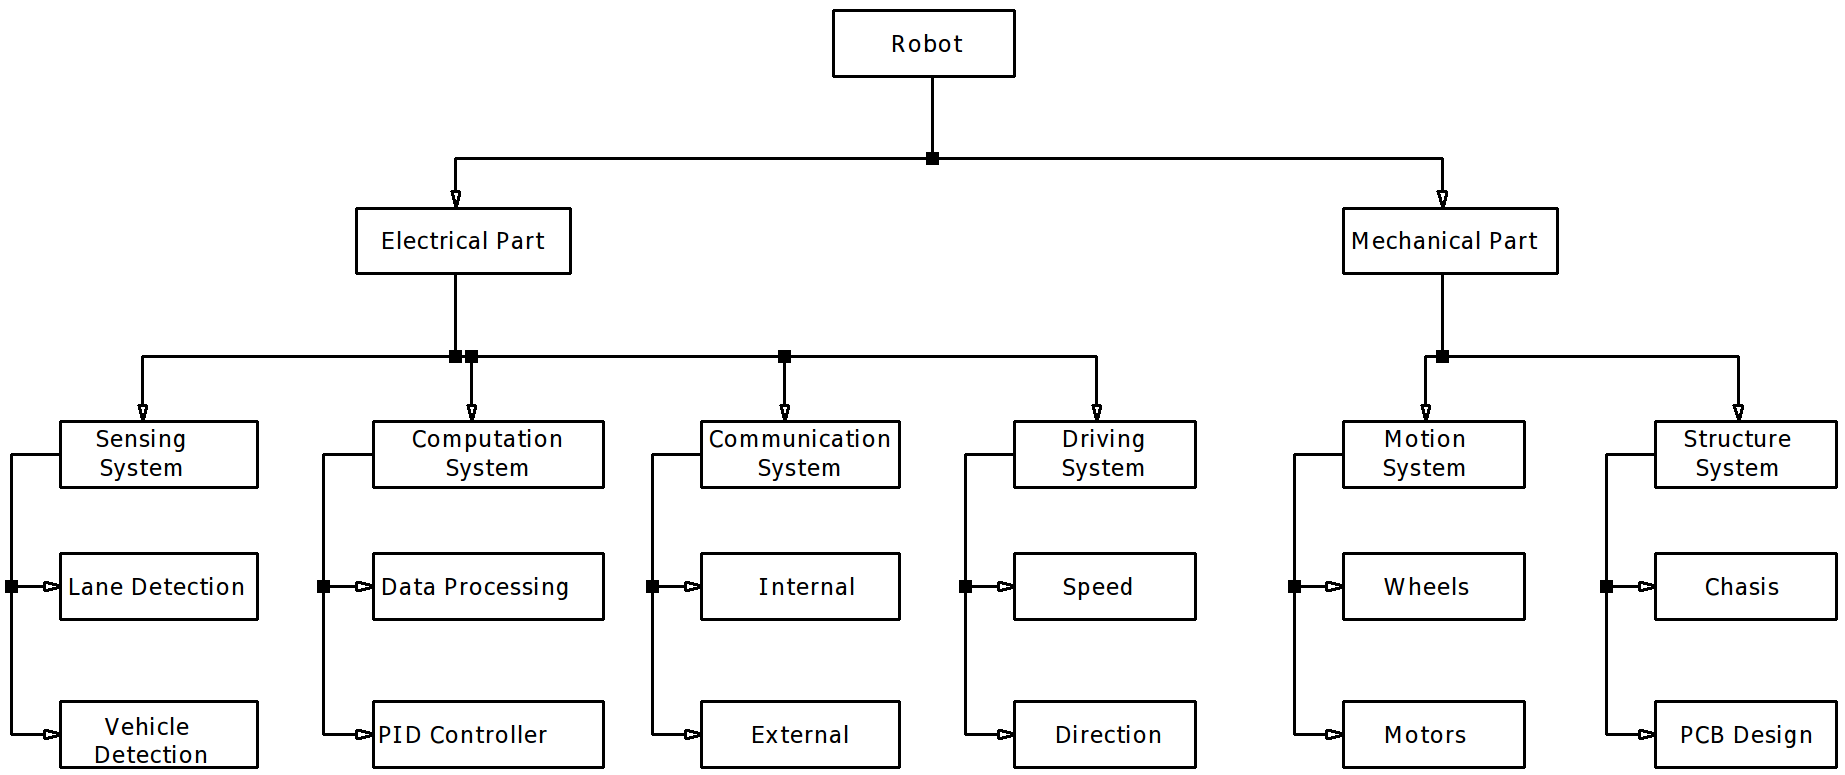
\includegraphics[width=\textwidth,center]{images/system}
		\caption{Organization of the Project}\label{fig:organization}
	\end{figure}

	V-Model provides a tool for companies to structure and track their product development processes. DUAYENLER constructed V-Model for the project as shown in \textit{Figure~\ref{fig:vmodel}}. 

	This section includes finalized system and subsystem level design descriptions. The ultimate algorithms, calculations, theoretical approaches and diagrams are presented in the related subsections.

	
	\begin{figure}[h]
		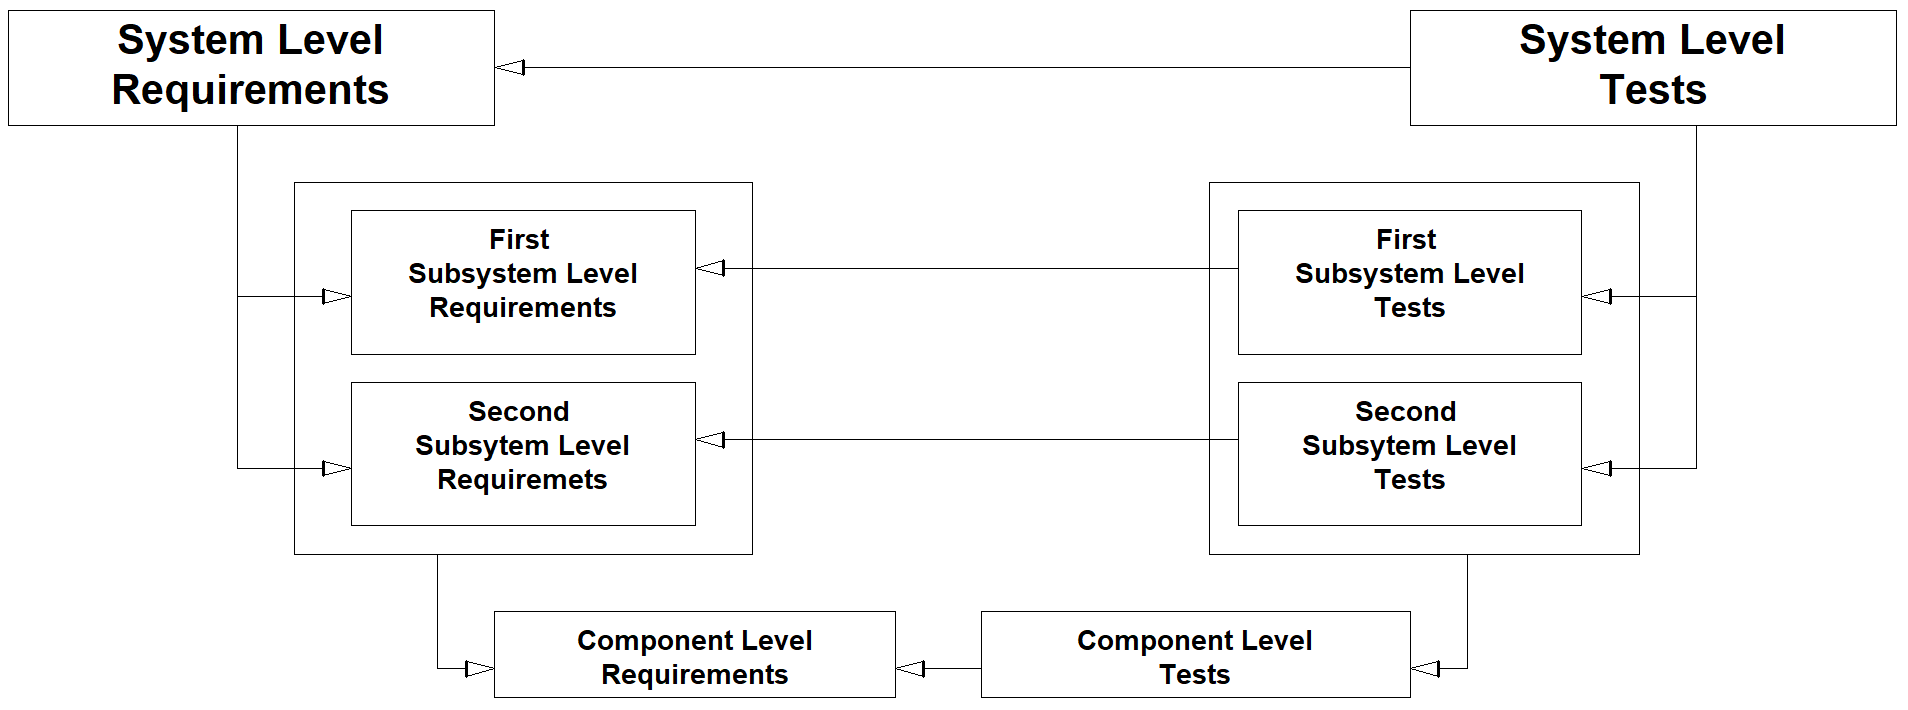
\includegraphics[width=\textwidth,center]{images/vModels/vmodel}
		\caption{V-Model}\label{fig:vmodel}
	\end{figure}

	%Besides, a Gannt Chart is prepared to have an detailed overview of future works and available in \textit{Appendix~\ref{gannt_chart_app}}.

%%%%%%%%%%%%%%%%%%%%%%%%%%%
%%%%%%%%%%%%%%%%%%%%%%%%%%%

\subsection{Sensing System}
	
	This system is responsible for interpreting data from the environment. And the requirements for this system are as follows;

	\begin{enumerate}
		\item The system should detect the sides of the road.
		\item The system should not be effected from external disturbances.
		\item The system should detect the opponent vehicle.
	\end{enumerate}	

	The system has two subsystems namely, 

	\begin{enumerate}
		\item \textbf{Lane Detection Subsystem} which is responsible for detecting sides of the path as its name suggests
		\item \textbf{Vehicle Detection Subsystem} which is responsible for detecting opponent vehicle if it is close to the vehicle more than 5 cm
	\end{enumerate}

%%%%%%%%%%%%%%%%%%%%%%%%%%%

\subsubsection{Lane Detection Subsystem}\label{sec:LaneDetectionSubsystem}

\begin{enumerate}[A.]

\item {Requirements for the Solution}




\begin{enumerate}[1)]

\item The subsystem should be able to detect only the shades of green color.

\item The subsystem should be able to detect edges in the camera frame in any light condition.

\item The subsystem should be able to extract lane lines out of captured frame.


\end{enumerate}




\begin{figure}[b]

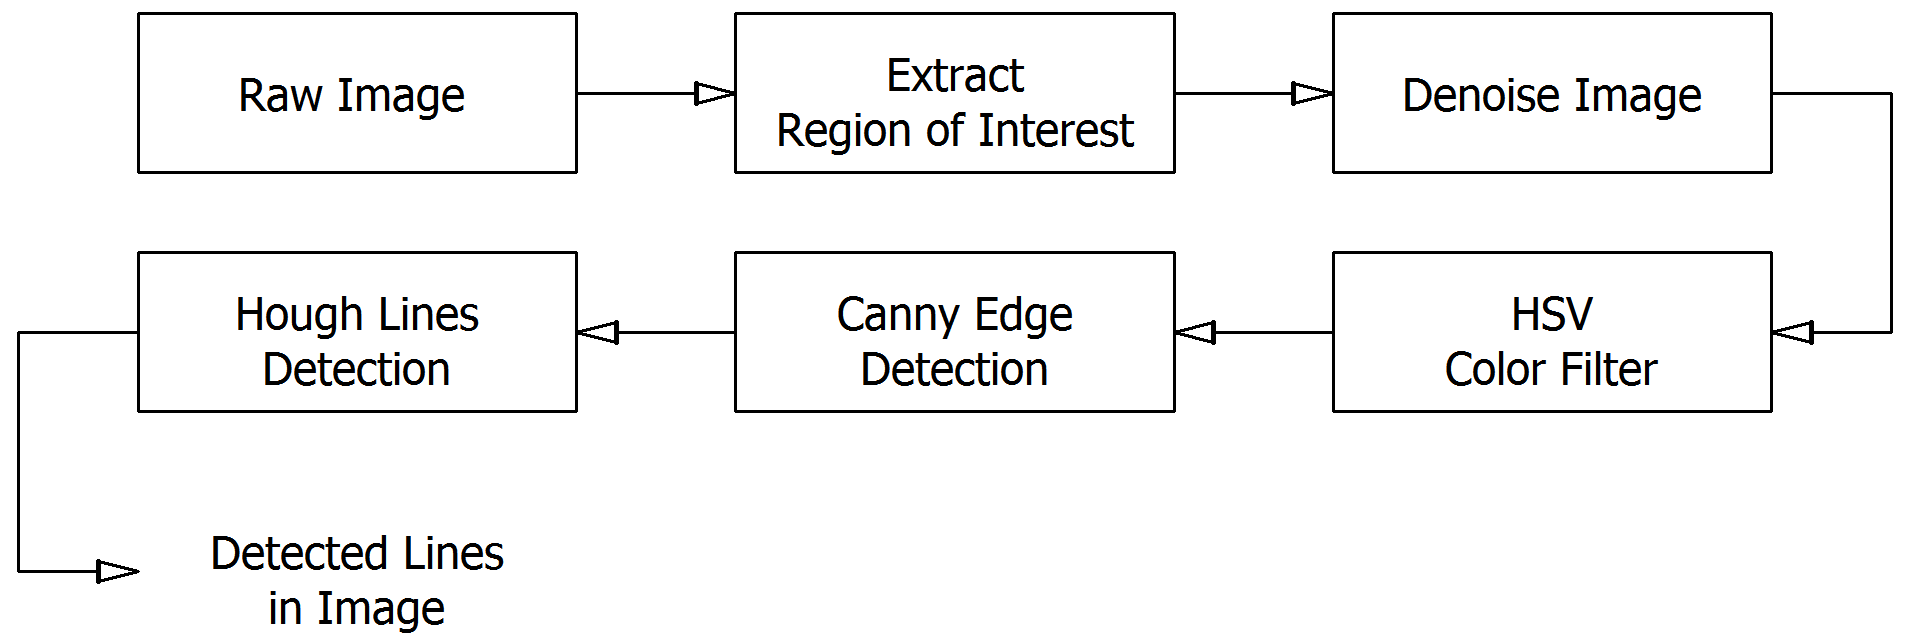
\includegraphics[width=0.93\textwidth,center]{images/vModels/laneDetection_subsystem}

\caption{Block Diagram of the Lane Detection Subsystem}\label{fig:lane_detection_subsystem}

\end{figure}




\item {Solution for the Subsystem}


The task of the subsystem is to detect the lane lines. The tool utilized to realize the task is OpenCV libraries together with developed pipelined algorithm. The block diagram of the subsystem is given in \textit{Figure~\ref{fig:lane_detection_subsystem}}.
\begin{figure}[t]
	
	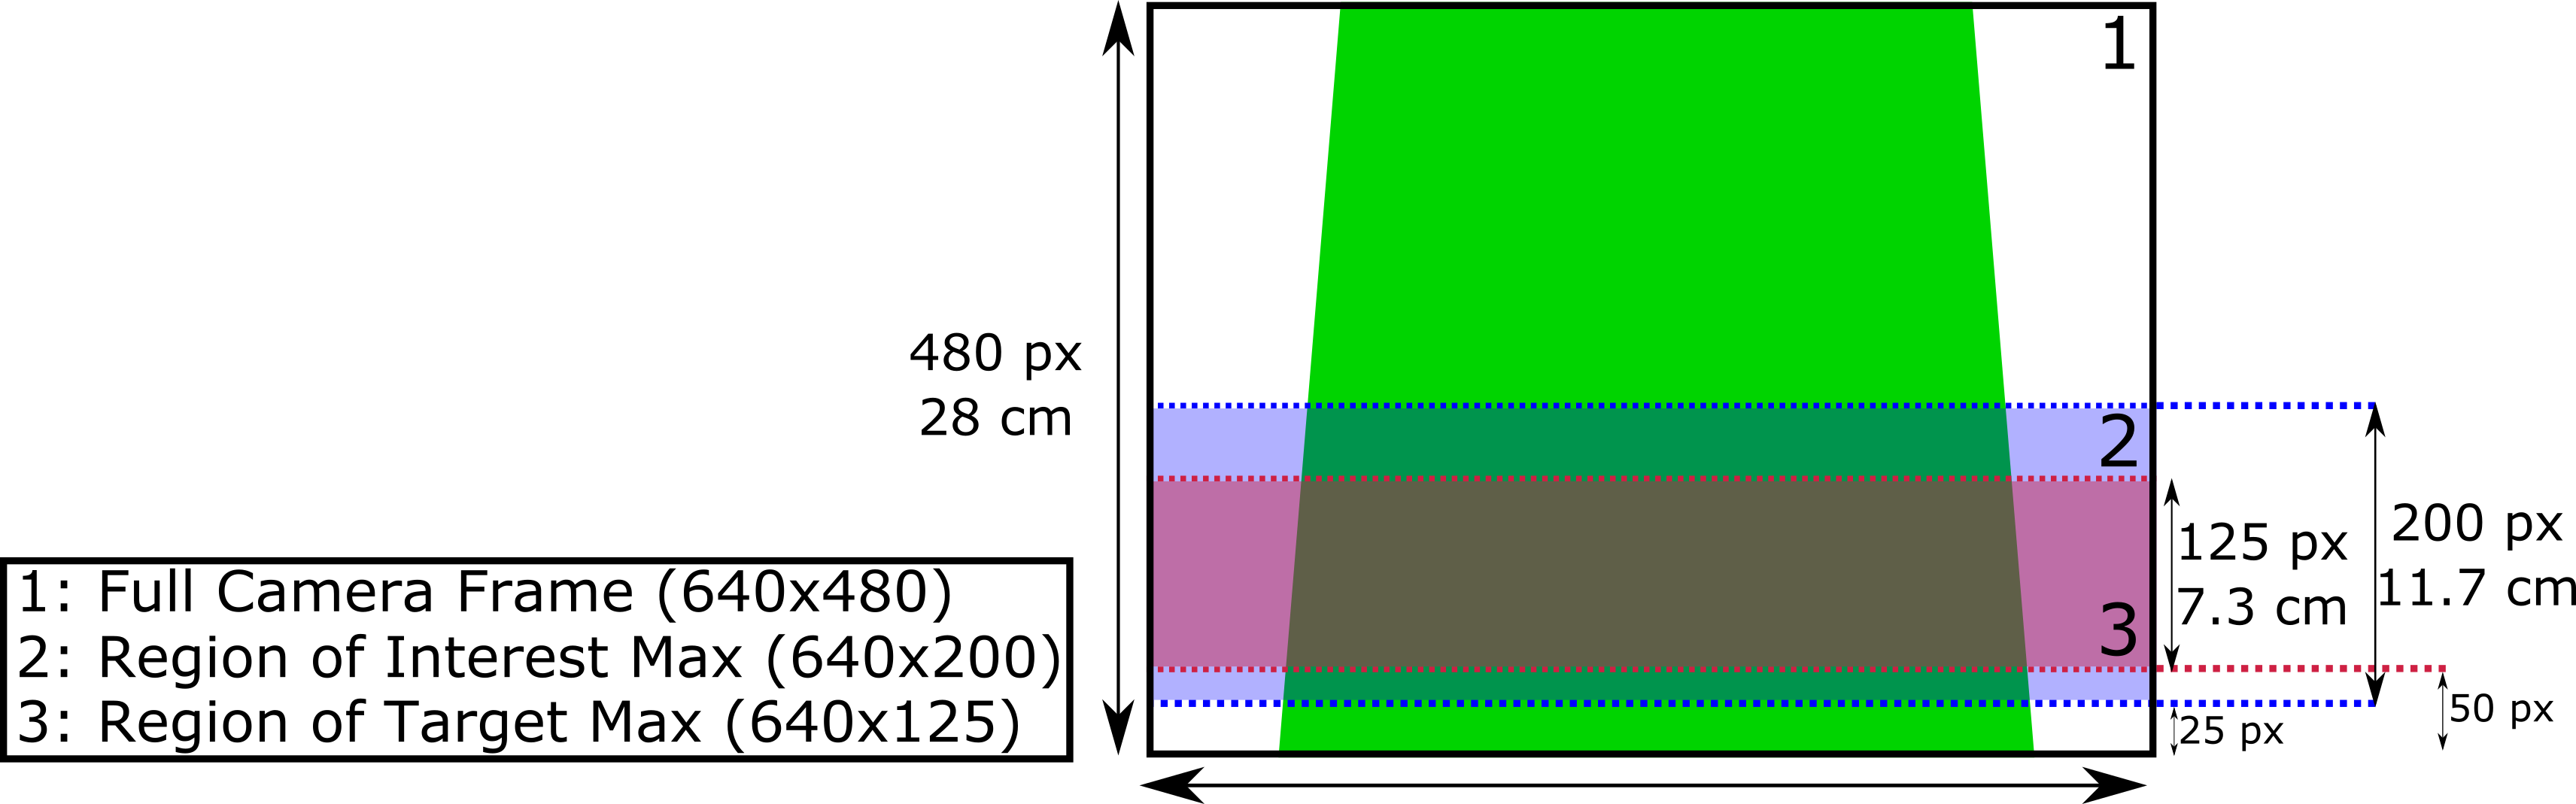
\includegraphics[width=0.93\textwidth,center]{images/ROT_ROI/explanation_ROI_ROT}
	
	\caption{Explanation of Frame Regions}\label{fig:explanation_ROI_ROT}
	
\end{figure}

The input to this subsystem is provided by Raspberry Pi camera mounted on top of the vehicle. The camera frame resolution is 640x480 px. One thing to for the camera frame is that horizontal mapping and the vertical mapping of the pixels are not the same. That is, same amount of pixels in both directions do not correspond to same length in real life. The proposed solution first masks out a region of interest (ROI) of $640x200 px$. The visual explanation of the frame sections is provided in \textit{Figure~\ref{fig:explanation_ROI_ROT}}. The masking eliminates the process of excessive data and increases the process speed of the pipeline. Formerly, ROI size was fixed in $640x200 px$. However, when the opponent vehicle starts to appear in ROI, this was causing wrong line detection in the subsystem. To eliminate such behaviour, adaptive ROI is implemented to avoid such improper situations. Adaptive ROI determines ROI size dynamically with the front distance sensor measurement provided by Vehicle Detection Subsystem and scales ROI size (only in vertical direction) with a linear function. The equations that define the height of ROI are as follows:
\begin{equation}
	ROI\_Width = 640 px
\end{equation}
\begin{equation}
	ROI\_Height = (ROI\_High - ROI\_Low) px
\end{equation}
\begin{equation}
	ROI\_Low = 25 px
\end{equation}
\begin{equation}
	ROI\_High =
		\begin{cases}
		225, & front\_distance \geq 13 cm \\
		14*(front\_distance) + 43, &3\leq front\_distance <  13 cm \\
		10*(front\_distance) + 55, & front\_distance \leq 3 cm
		\end{cases}
\end{equation}
The graphical representation of the equations are given in \textit{Figure~\ref{fig:ROI_crop}}


\begin{figure}[t!]
	
	\setlength{\unitlength}{\textwidth} 
	
	\centering
	
	\begin{subfigure}{.46\textwidth}
		
		\centering
		
		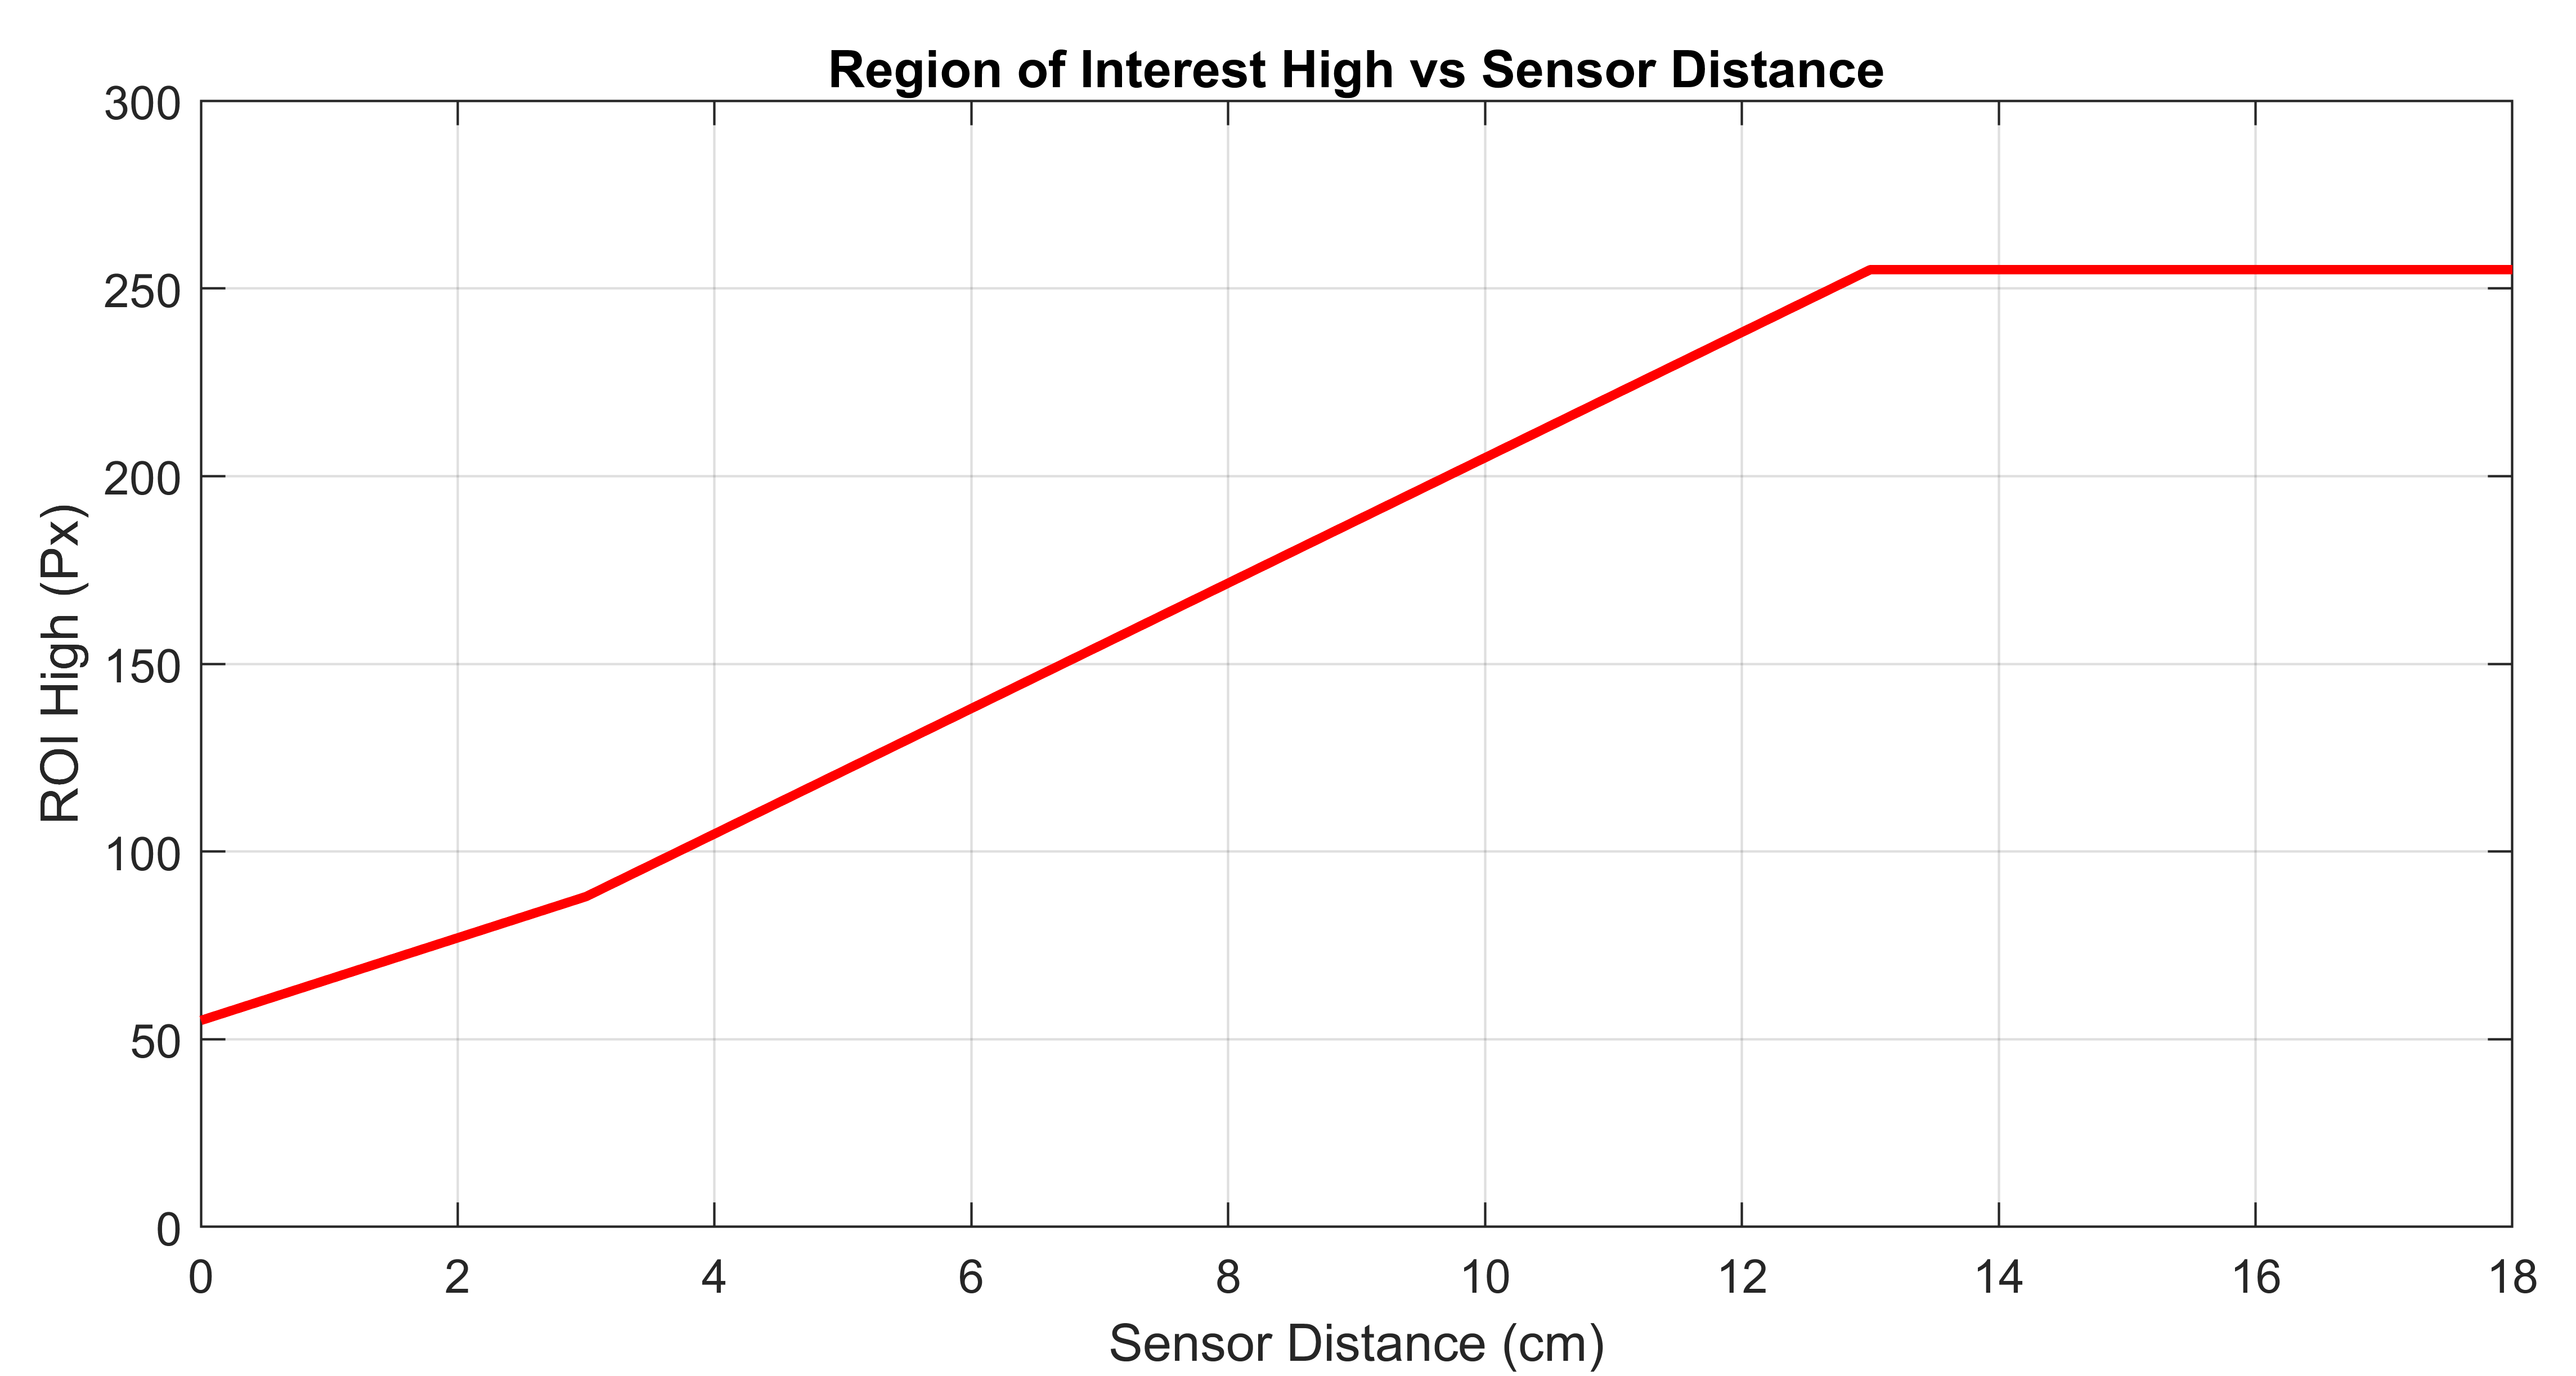
\includegraphics[width=0.44\unitlength]{images/ROT_ROI/ROI_HIGH_crop}
		
		\caption{ Graph of ROI\_High vs front\_distance}
		
	\end{subfigure}%
	\begin{subfigure}{.46\textwidth}
		
		\centering
		
		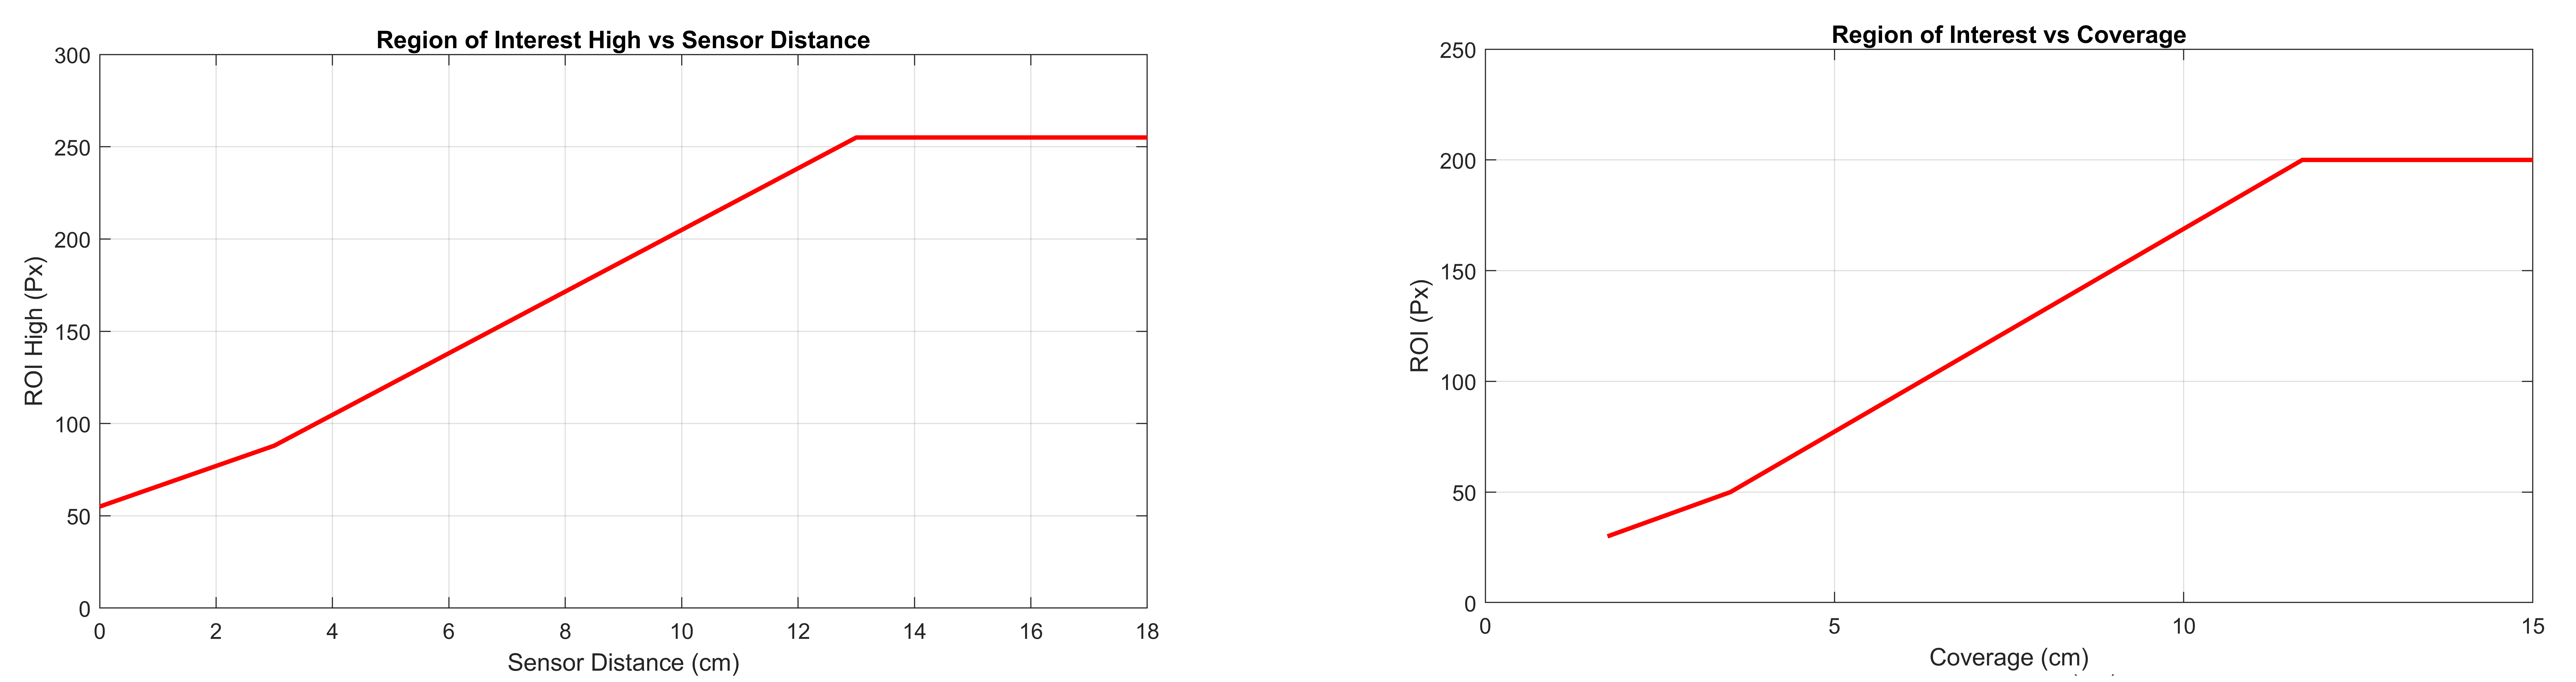
\includegraphics[width=0.44\unitlength]{images/ROT_ROI/ROI_crop}
		
		\caption{ ROI\_Height Variation}
		
	\end{subfigure}
	
	\caption{\label{fig:ROI_crop} Graphs Defining ROI\_Height}
	
\end{figure}

As the next step of the processing pipeline, the target color green is filtered by applying Gaussian denoise (with zero mean) and HSV filters. The lower bound for HSV filter is [H=60, S=120, V=106] and the upper bound is [H=82, S=255, V=245]. This process sets the pixels that are in the green threshold to white and the rest to black. Next, the edges are detected by Canny edge detector. As edges are found, the pixels that may constitute a line are found by Hough line detector. The resulting output is an array of coordinates in the form of $[x_1, y_1, x_2, y_2]$ where $(x_1, y_1)$ is the starting point of the line and $(x_2, y_2)$ is the end point of the line. The found coordinate array is passed to Data Processing Subsystem.





\item {Discussions on the Solution}


The main structure of the proposed solution has not changed since Conceptual Design Review Report. An addition to process pipeline is introducing adaptive ROI. This is done to be able to follow opponent vehicle on the back.

For this subsystem to be stable, HSV filter must produce a clean filtered result. The filter is responsive as long as it is tuned according to light condition.

%This is done to both improve the performance and remove possible distractions that are present in the image. A point to note in this algorithm is Hough line detector. It is a probabilistic function, meaning that even if the captured frame is the same as previous frame, the found line coordinates may differentiate a bit. However, this is not a big issue. One weak point was the lane detection under extreme lighting conditions. The filter is adjusted to be able to detect in bright lighting conditions but dark lighting is problematic. To solve this issue, the team decided to place LED strips to front bumper of the vehicle.


\end{enumerate}



%%%%%%%%%%%%%%%%%%%%%%%%%%%

\subsubsection{Vehicle Detection Subsystem}

\begin{enumerate}
	\item {Requirements for the Solution}
	
	\begin{enumerate}
		\item The subsystem should detect the opponent to be caught with in a 5 cm 
		\item The subsystem should detect the chasing opponent if it reaches from back with in a 5 cm 
		\item The subsystem should trigger the handshake protocol 
	\end{enumerate}
	
	\item {Solution for the Subsystem}
	
	The subsystem is the first step of safely competing with an opponent in a racing path. This subsystem uses two time of flight distance sensors, called vl6180x. Time of flight sensors are enhanced IR sensors. One at the back of the vehicle is responsible for detecting the chasing opponent and one at the front of the vehicle is responsible for detecting the chased opponent. The sensors use I2C protocol. The serial data coming from sensors is between 0 and 255, which corresponds to the reading in terms of millimeters. That is, vl6180x can make measurements up to 25.5 cm. Since sensor reading is performed using Raspberry Pi, the required trigger for handshake protocol can be easily accessed by the external communication subsystem.
	
	Note that, having 2 sensors means that there are 2 I2C slaves. In I2C, master device sends data to slaves according to their addresses. The main problem emerging from this is that if two sensors have the same address, reading sensors is not possible. Therefore, the addresses of the sensors must be changed. However, there is also another problem. Changing address is also done by sending serial data to sensors. If both sensors are connected at the same time to Raspberry Pi, changing addresses is not possible because there are still 2 devices with same addresses. To solve this issue, the chip enable(CE) inputs of the sensors is used. Firstly, only one device is activated by applying high to its CE input pin. After changing its address, other sensor's CE pin can be safely made high. By doing that, two I2C devices with different addresses are obtained. From this point on, sensors can be read successfully.
	
	\item {Discussions on the Solution}
	
	The proposed method is not changed after Critical Design Review Report. Changing I2C slave addresses is done to successfully use both sensors. Also, the sensor readings are integrated to handshake code.
	
	
\end{enumerate}


%%%%%%%%%%%%%%%%%%%%%%%%%%%	
%%%%%%%%%%%%%%%%%%%%%%%%%%%


\subsection{Computation System}


This system is responsible for computational works of the vehicle. The system mainly give meaning to data generated by the sensing system. The requirements for this system are as follows: 


\begin{itemize}

\item The system should	be able to produce middle line to follow

\item The system should be able to control the robot

\end{itemize}	


\noindent The system has two subsystems namely,


\begin{enumerate}

\item \textbf{Data Processing Subsystem} is responsible for processing the output data of lane detection unit and produce data for PID control unit.

\item \textbf{PID Controller Subsystem} is responsible for controlling the motors of the vehicle.

\end{enumerate}




\subsubsection{Data Processing Subsystem}\label{sect:dataProcessingSubsystem}

\begin{enumerate}[A.]

\item {Requirements for the Solution}


\begin{enumerate}[1)]

\item The subsystem should be able to analyze data produced by Sensing System.

\item The subsystem should be able to produce the angle information that is sent to the Controller Subsystem.

\item The subsystem should be compatible with Raspberry Pi.

\item The subsystem should be able to process one frame at most in 100 milliseconds together with Lane Detection Subsystem.

\item The subsystem should be able to ignore disturbances on the path.

\end{enumerate}


\item {Solution for the Subsystem}

\begin{figure}[h]

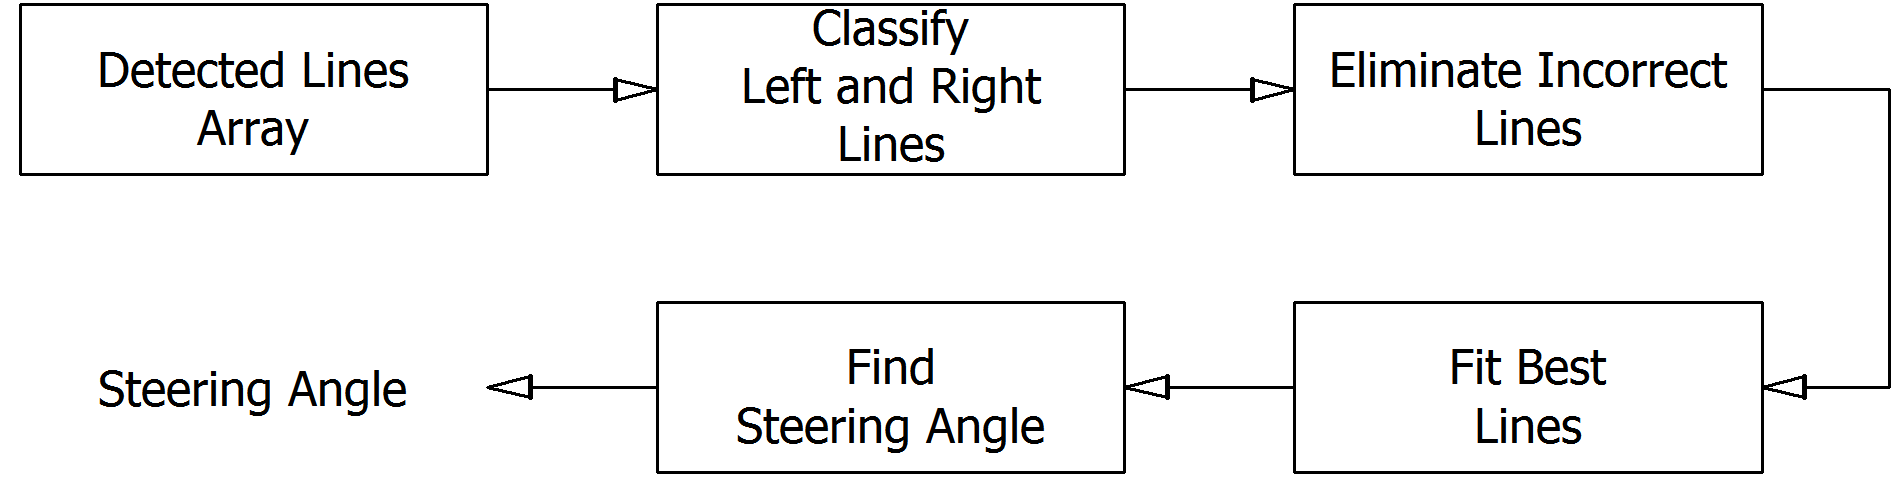
\includegraphics[width=0.93\textwidth,center]{images/vModels/dataProcessing_subsystem}

\caption{Block Diagram of the Data Processing Subsystem}\label{fig:dataProcessing_subsystem}

\end{figure}



	The task of this subsystem is to extract control parameters so that the vehicle can follow the path without falling on the ground. The input of the subsystem is the line coordinate array produced by Lane Detection Subsystem. The input is processed by a detailed algorithm and the outputs are lane angle and distance of vehicle to the right lane. The output parameters are explained in \ref{sect:ControllerSubsystem}. The outputs are generated for the region of target (ROT) that is shown in \textit{Figure~\ref{fig:explanation_ROI_ROT}}. The Lane Detection Subsystem extracted ROI out of full camera frame. The Data Processing Subsystem processes the data in the ROI but produces output for the ROT. The reason for such a distinction between frame regions is that, ROI is good to determine possible obstacles on the path but producing control outputs that are almost 12 cm away from the vehicle would decrease the performance of the PID Controller Subsystem. For this reason ROI is not used, instead ROT is used. As ROI is adaptive, ROT must also be adaptive to stay in ROI region. The equations that define the ROT are as below. The graphical representation of the equations are given in \textit{Figure~\ref{fig:ROT_crop}}.
\begin{equation}
ROT\_Width = 640 px
\end{equation}
\begin{equation}
ROT\_Height = (ROT\_High - ROT\_Low) px
\end{equation}
\begin{equation}
ROT\_Low = 50 px
\end{equation}
\begin{equation}
ROT\_High =
\begin{cases}
175, & front\_distance \geq 13 cm \\
10*(front\_distance) + 45, &3\leq front\_distance <  13 cm \\
21*(front\_distance) + 12, & front\_distance \leq 3 cm
\end{cases}
\end{equation}
\begin{figure}[t!]
	
	\setlength{\unitlength}{\textwidth} 
		\centering
		\begin{subfigure}{.46\textwidth}
			\centering
			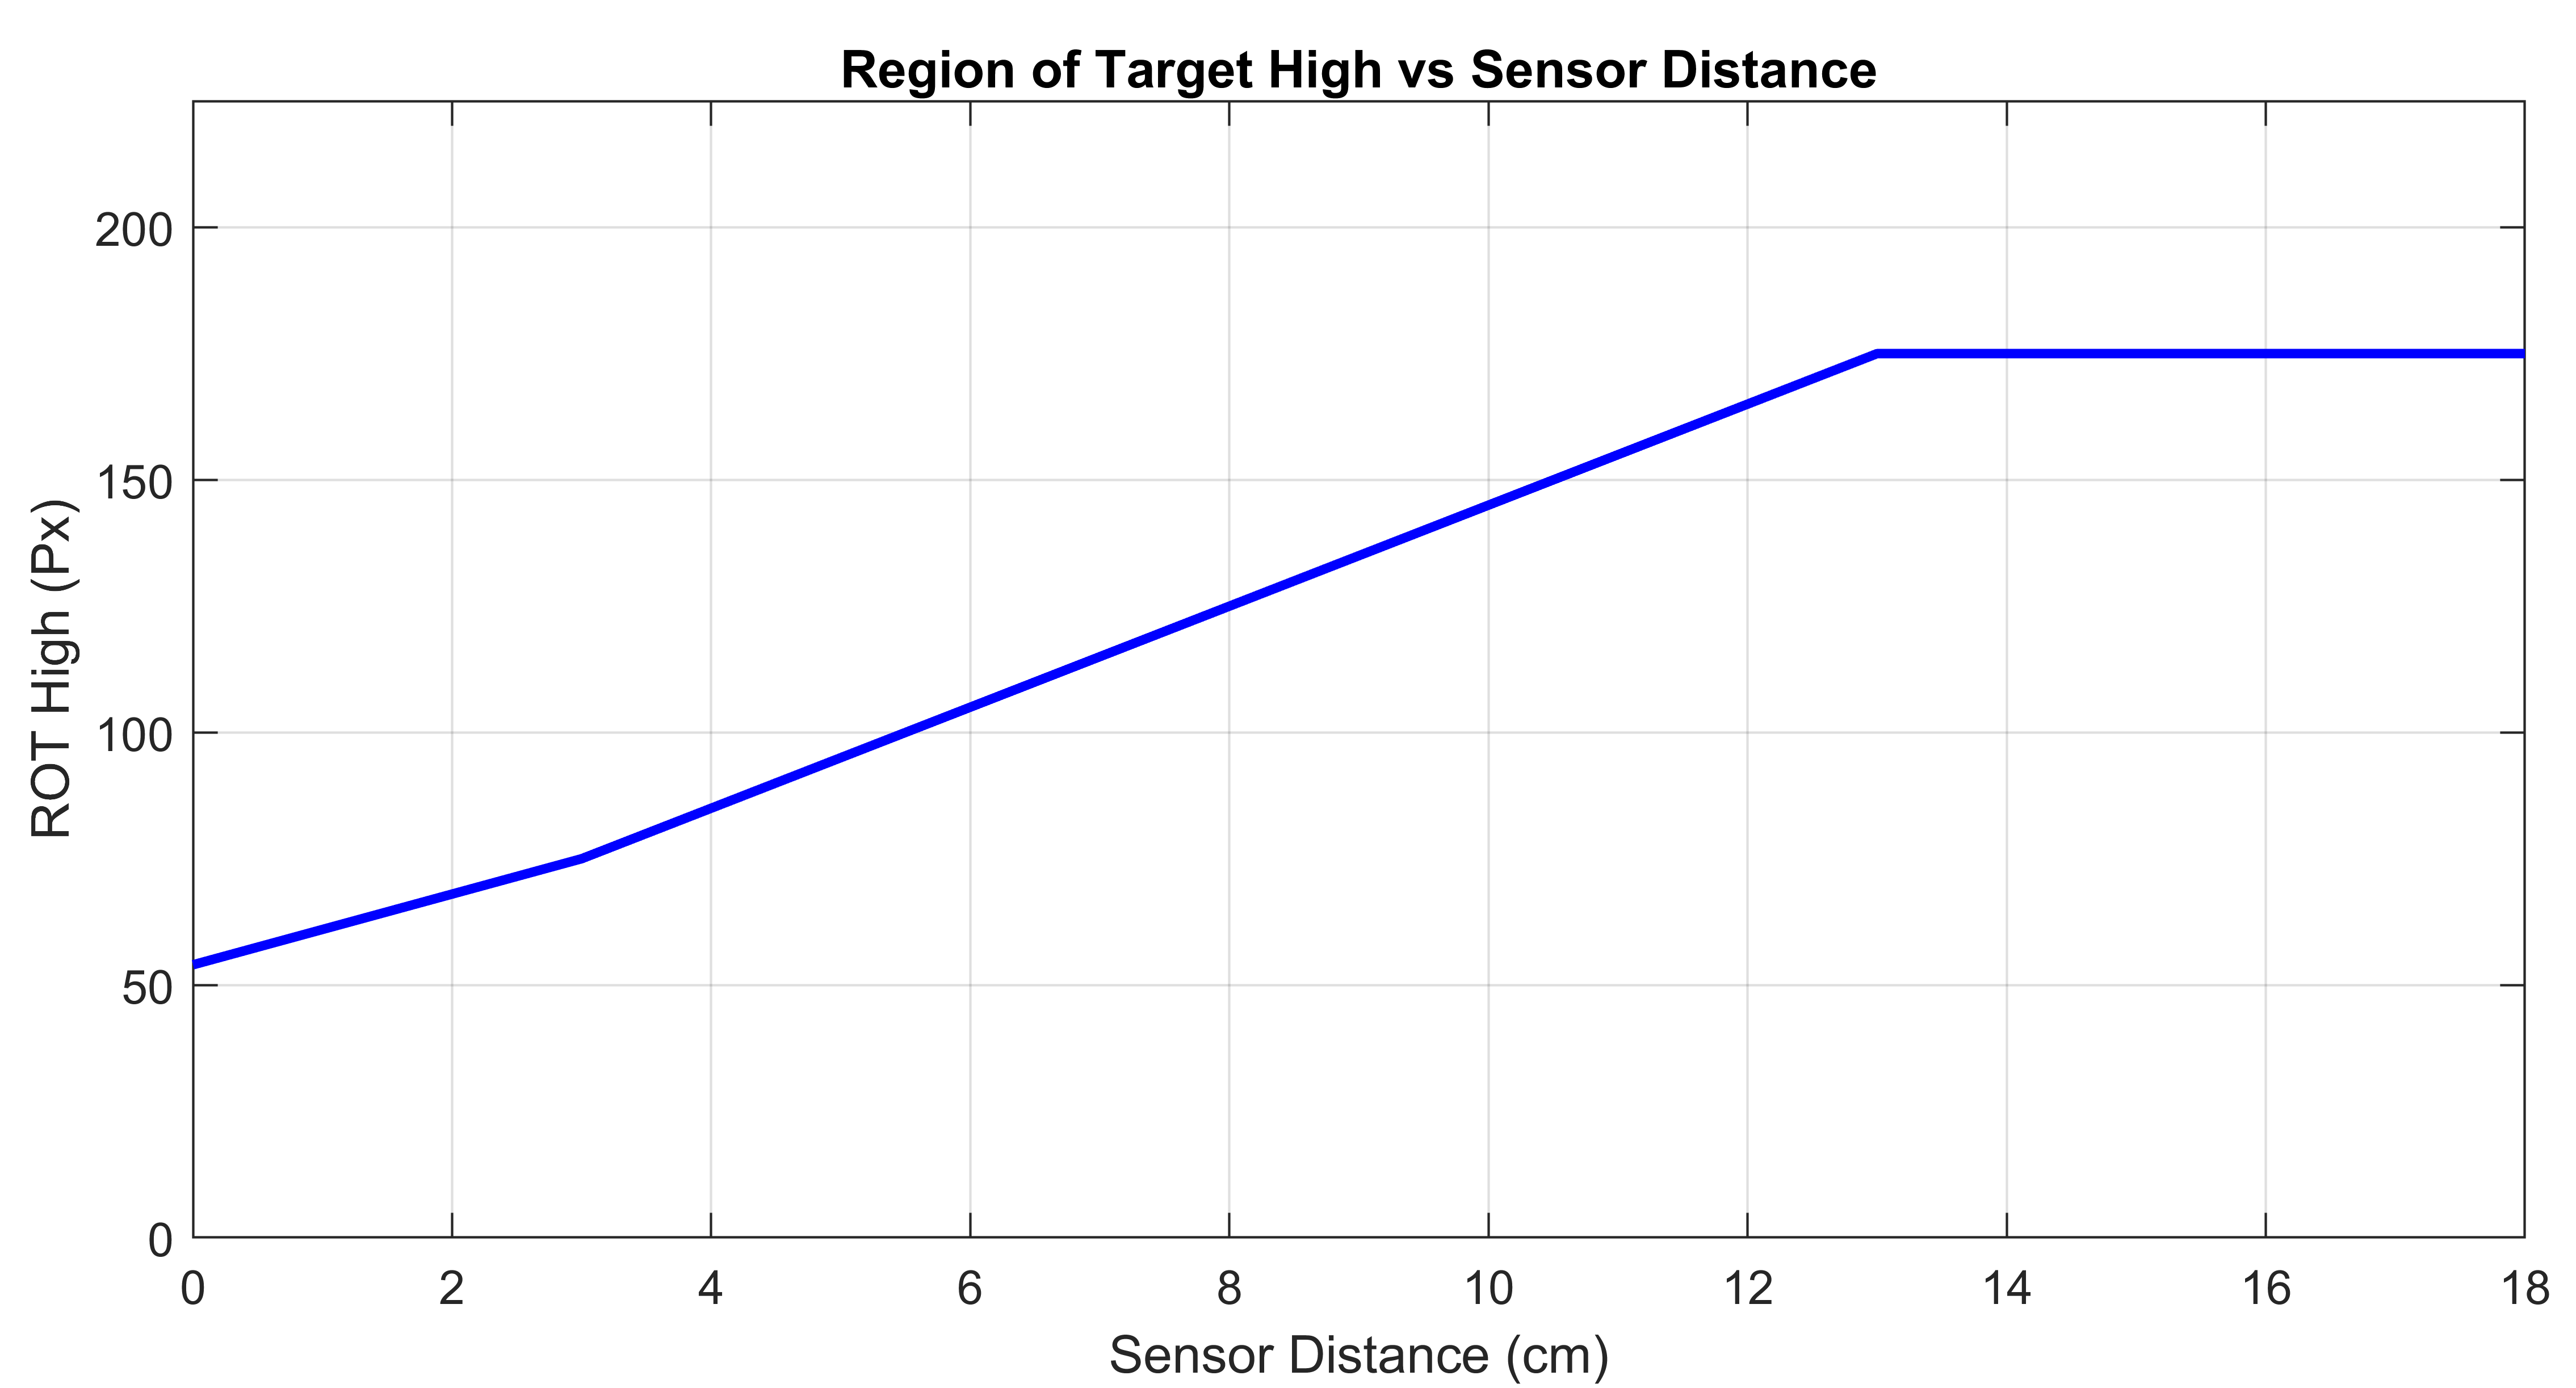
\includegraphics[width=0.44\unitlength]{images/ROT_ROI/ROT_HIGH_crop}
			\caption{ Graph of ROT\_High vs front\_distance}
		\end{subfigure}%
		\begin{subfigure}{.46\textwidth}
			\centering
			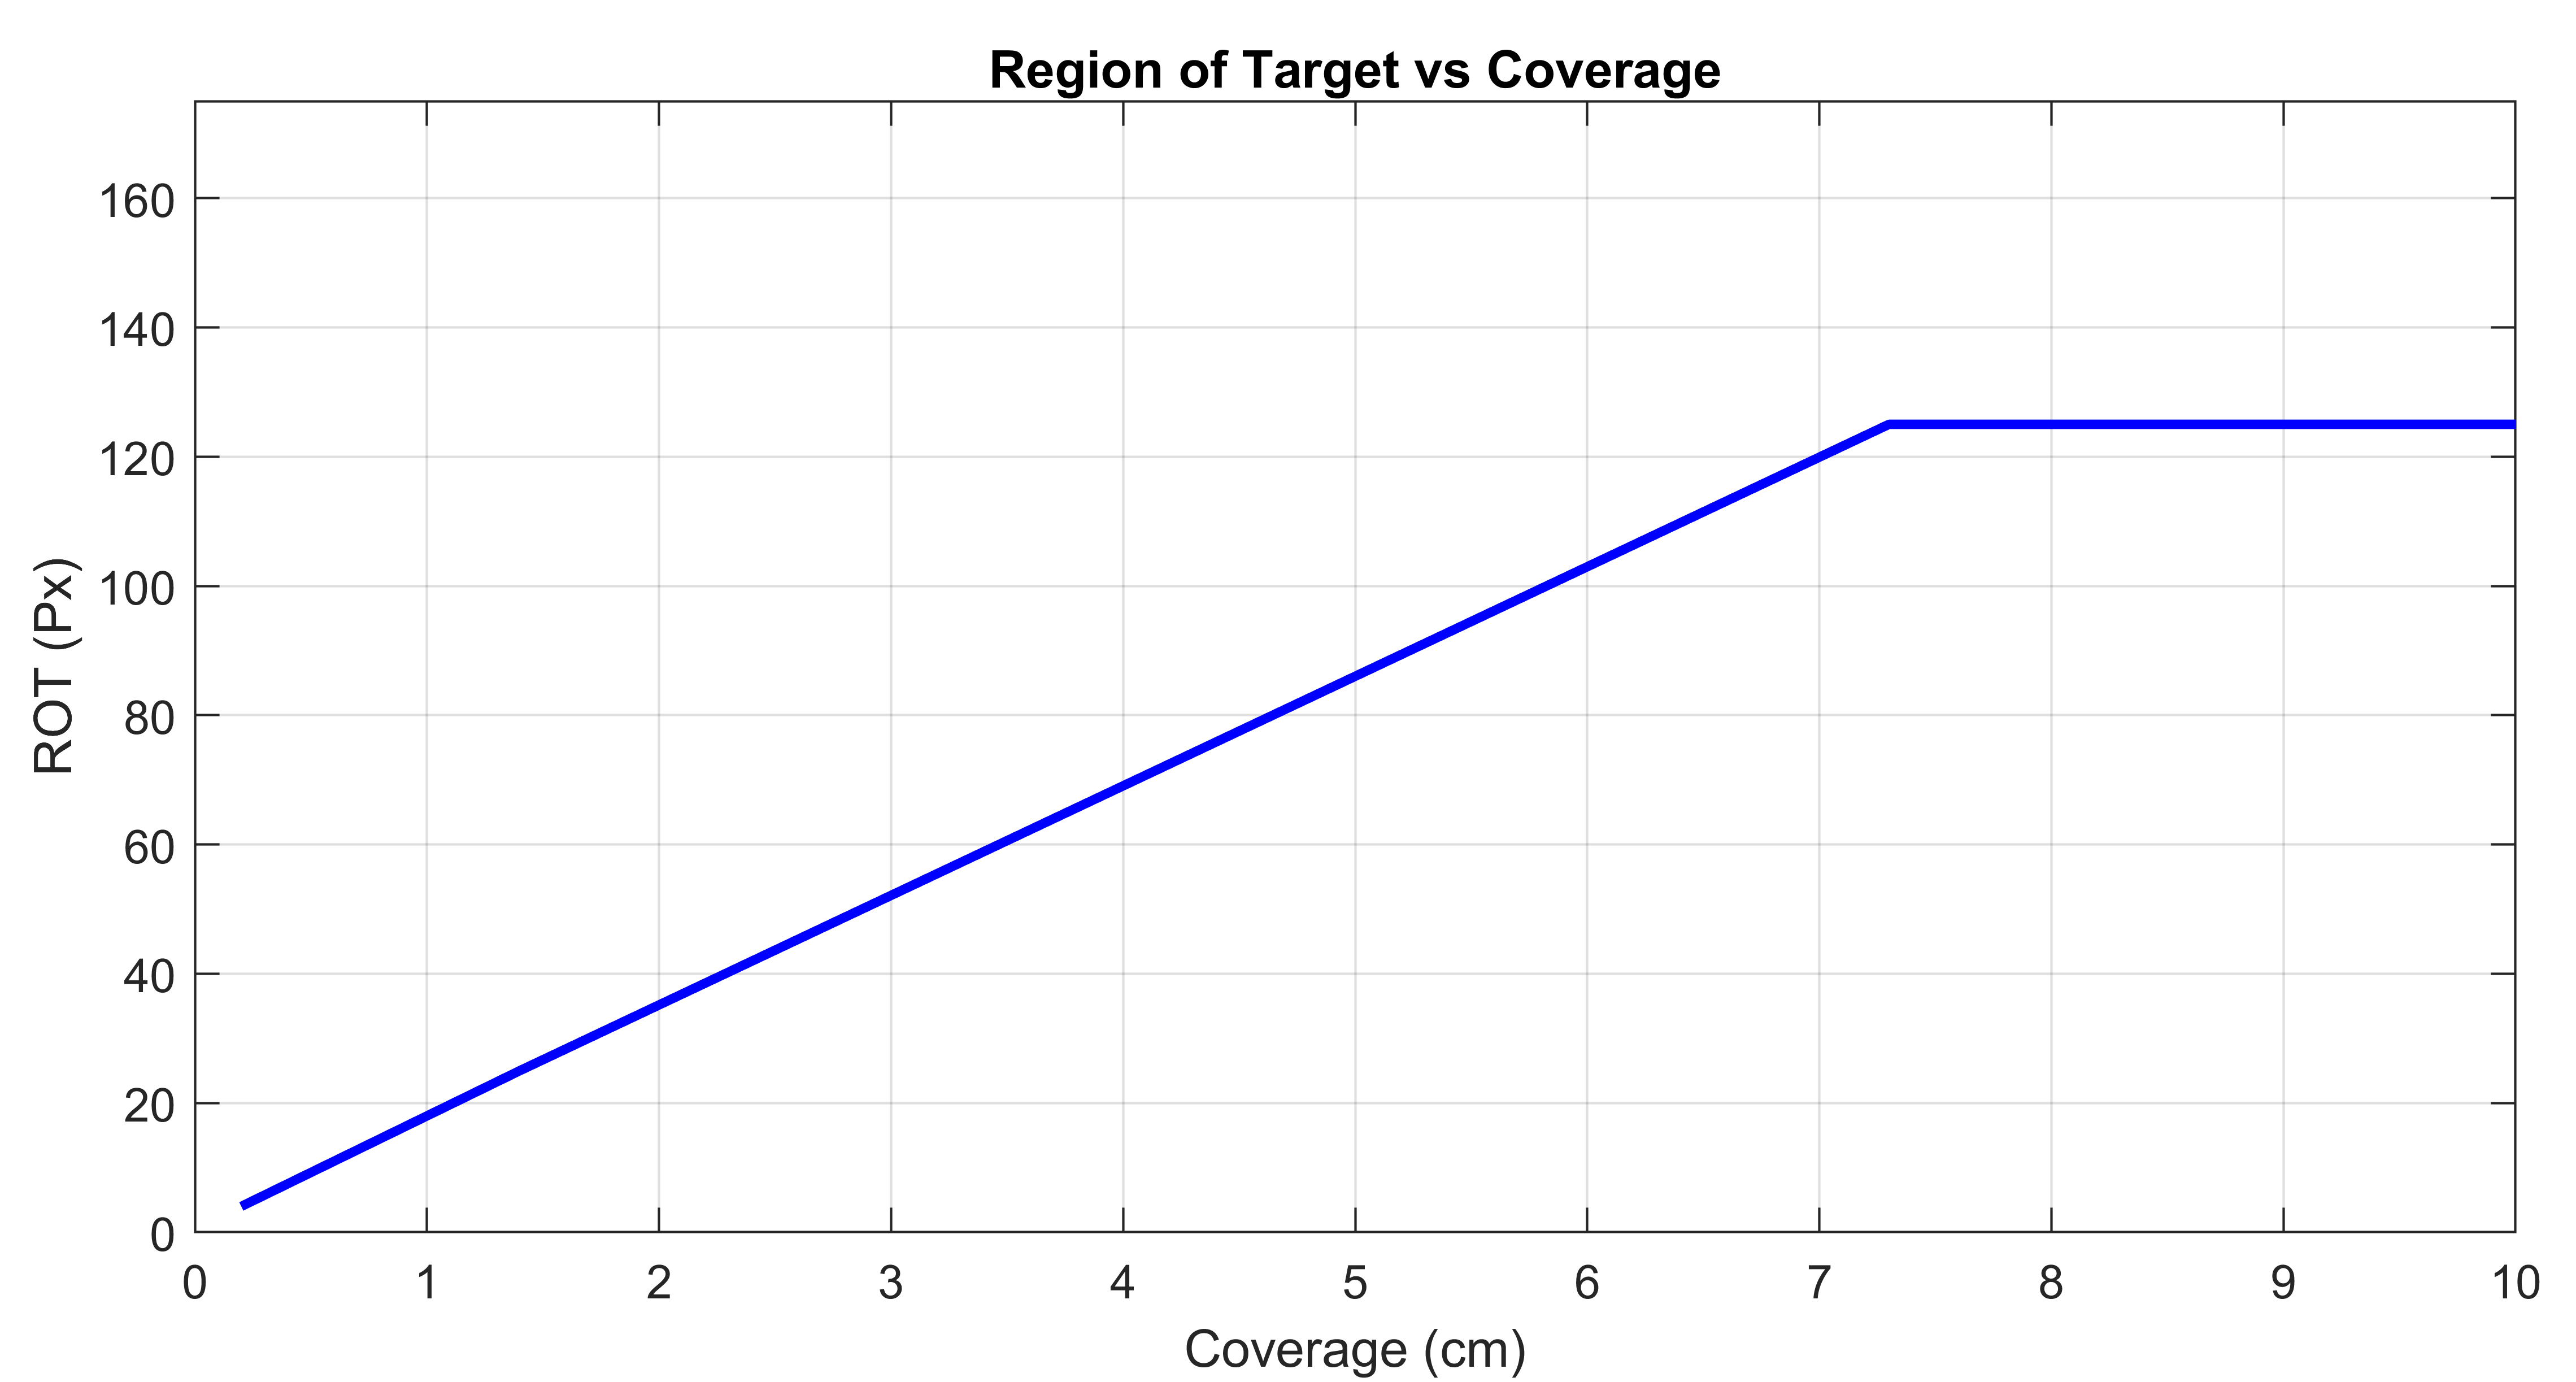
\includegraphics[width=0.44\unitlength]{images/ROT_ROI/ROT_crop}
			\caption{ ROT\_Height Variation}
		\end{subfigure}
		\caption{\label{fig:ROT_crop} Graphs Defining ROT\_Height}
	\end{figure}

	There are four main steps to determine lane angle and distance of vehicle to the right lane. The first step is to classify the lines as left and right. The second step is to eliminate the possible incorrect lines, if any. The third step is to fit the best lines through the left and right lines and reduce the total number of lines to two that are left and right lane lines. The last step is to find control outputs. The block diagram of the subsystem is given in \textit{Figure~\ref{fig:dataProcessing_subsystem}}.

	Classifying a line as left or right requires the knowledge of the center of the path. If a pixel is part of the path, it is indicated by pixel value 255, that is result of HSV filtering. So, the path is constructed by white pixels. Analogously, if white pixels on a column is counted, that counts yield an information regarding the start and end points of the path. The explanation will be made based on an example frame (with ROI masked) as in \textit{Figure~\ref{fig:explanation_center_of_image}}. Obviously, the white pixel count through every column in the arrow directions between red bars is 0. However, from red bars to yellow bars, white pixel count in columns starts to increase. The maximum pixel count in a column is known from ROI equations. If the column indices that are close to maximum pixel count in a columns can be determined, then the right and left bounds of the path are found. Then, the center of the image is simply $(right\_bound + left\_bound)/2$. \textit{Algorithm~\ref{algo:center_image}}. As the center of the image is found, lines can be separated as left or right according to their coordinates.

\begin{figure}[h]
	
	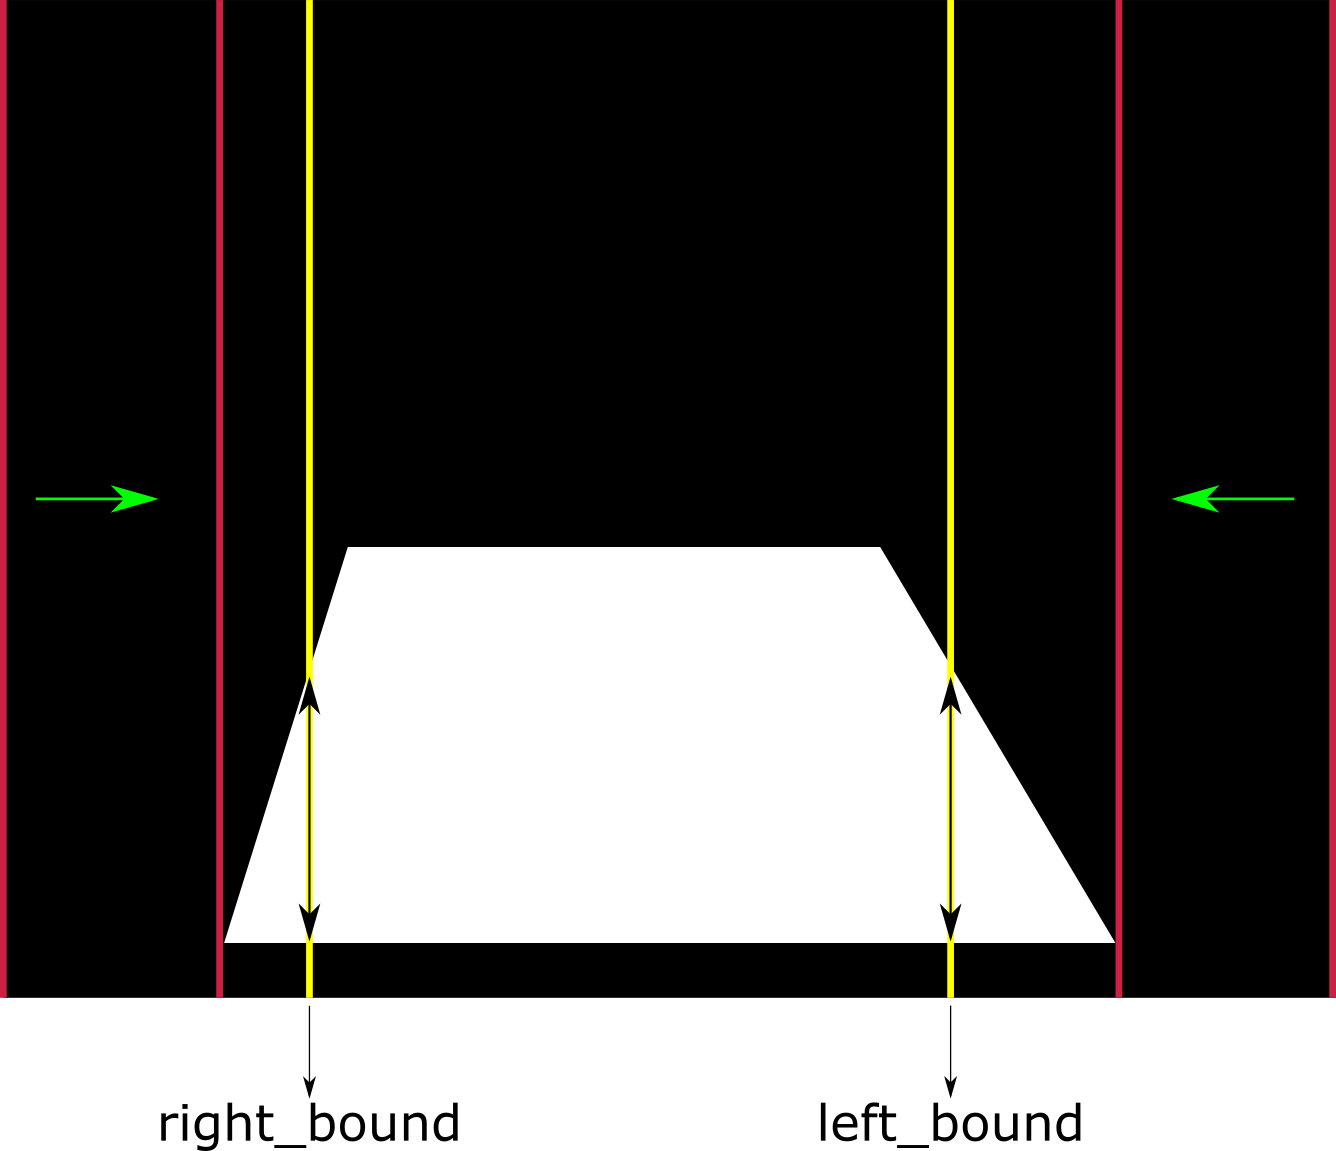
\includegraphics[width=0.465\textwidth,center]{images/ROT_ROI/explanation_center_of_image}
	
	\caption{Finding Center of the Path}\label{fig:explanation_center_of_image}
	
\end{figure}
\begin{algorithm}
	\DontPrintSemicolon
		$whitePixels[640]$\;

		$confidenceCount = 190 // threshold Pixel Count$\;

		\For{Every Row i}{
			\For{Every Column j}{
				\If{frame[i][j] == 255}{
					$whitePixels[j]++$\;

				}
				
			}
		}
	
		\For{Elements of whitePixels from left to right}{
			Find the first index that has white pixel count greater than confidenceCount;

			That index is left\_bound;

		}
		
	\For{Elements of whitePixels from right to left}{
		Find the first index that has white pixel count greater than confidenceCount;
		That index is right\_bound;
	}

	image\_center = (left\_bound + right\_bound)/2
	

	\caption{Finding Image Center\label{algo:center_image}}
\end{algorithm}

\begin{figure}[t!]

\setlength{\unitlength}{\textwidth} 

\centering

\begin{subfigure}{.46\textwidth}

\centering

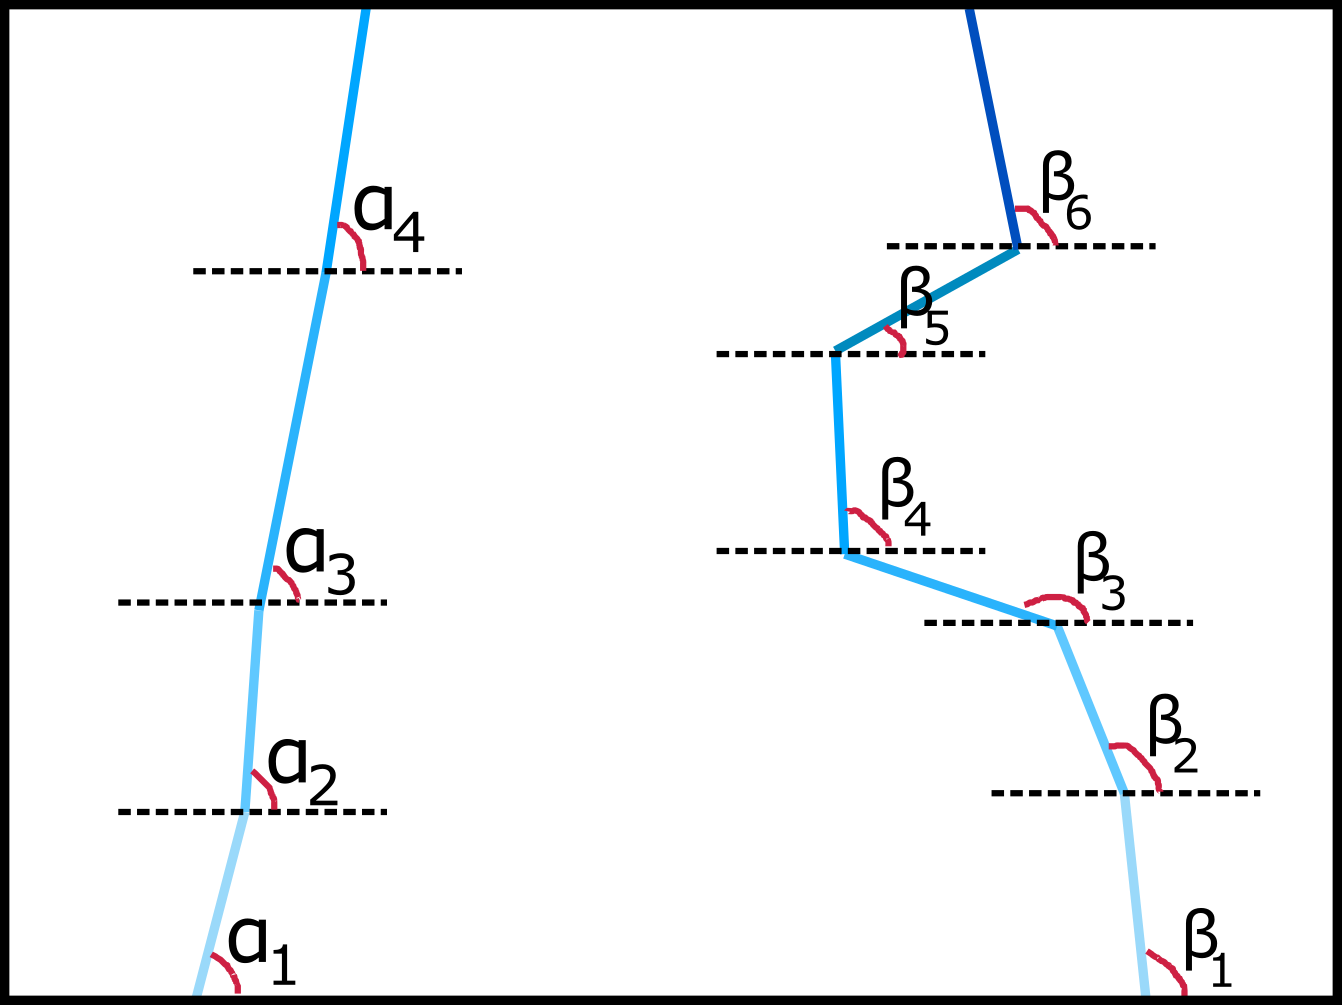
\includegraphics[width=0.44\unitlength]{images/dataP_explained1}

\caption{\label{fig:dataP_explained1} Before Eliminating Incorrect Lines}

\end{subfigure}%
\begin{subfigure}{.46\textwidth}

\centering

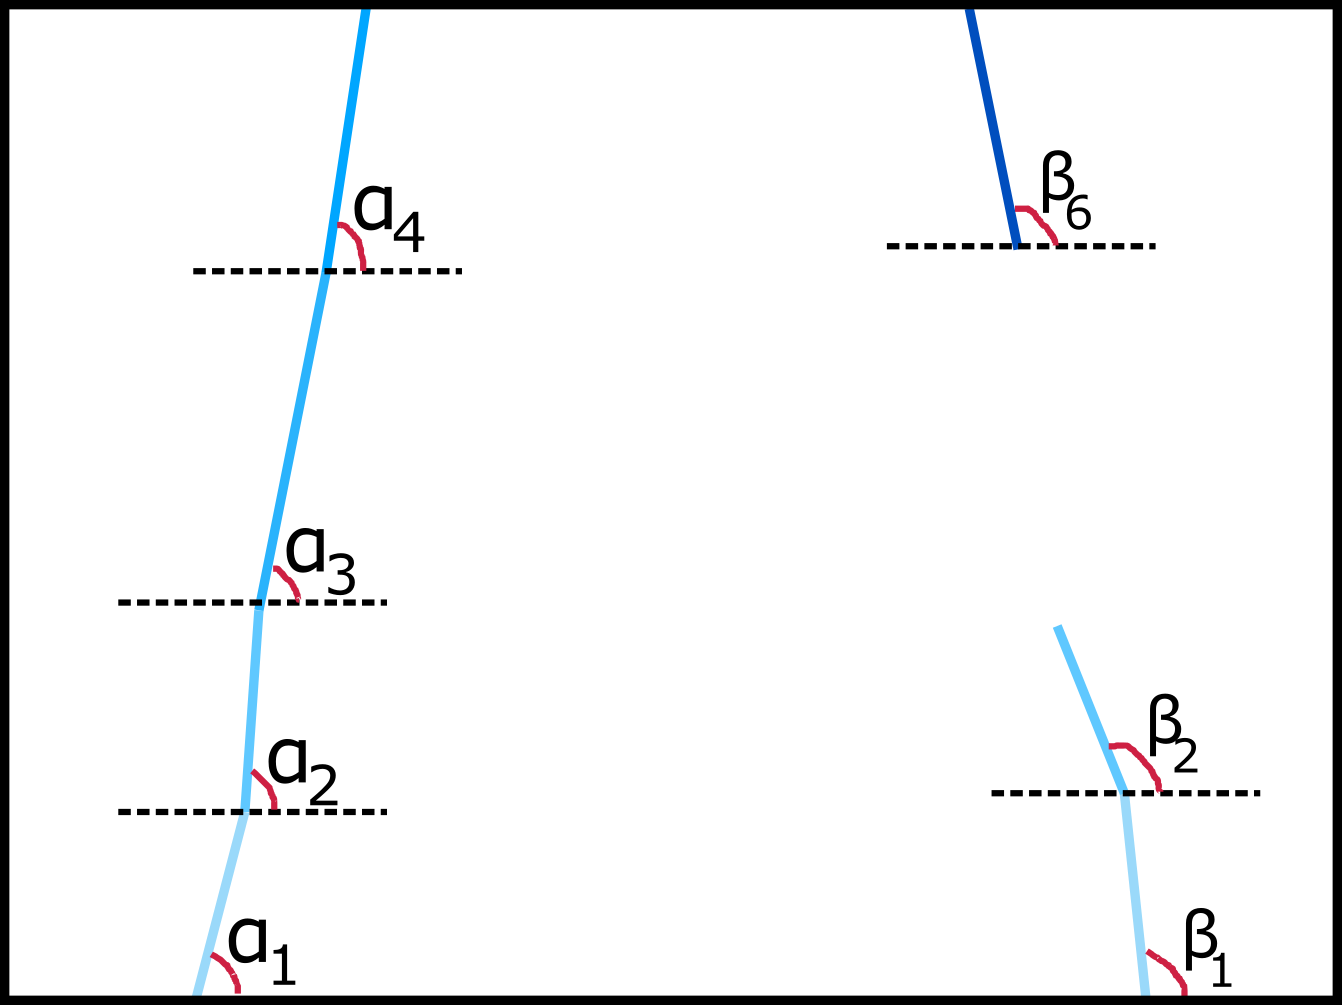
\includegraphics[width=0.44\unitlength]{images/dataP_explained2}

\caption{\label{fig:dataP_explained2} After Eliminating Incorrect Lines}

\end{subfigure}

\caption{\label{fig:dataP_explained} A Sample Scenario on Eliminating Incorrect Lines}

\end{figure}





The next step is to determine whether there are disturbances on the lane lines or not. This is the most complex part of the Data Processing subsystem. Actually the correctness of the steering angle depends on how successful this step is realized. The idea behind this step is evaluating the slopes consecutive lines and assessing whether change in the slope is ordinary or abnormal. The \textit{Figure~\ref{fig:dataP_explained}} exemplifies a possible scenario. In this figure, the blue lines represent the detected lines in ROI whereas $\alpha$ and $\beta$ represent the slopes of the detected lines. Clearly, there are no disturbance on left lines since $\alpha$ values are similar to each other. However if $\beta$ values are observed, possibly there is an obstacle on right line covered by $\beta_3$, $\beta_4$ and $\beta_5$. This can be concluded by observing slope differences $(\beta_2 - \beta_3)$ and $(\beta_5 - \beta_6)$. To ignore this obstacle, it is enough to remove lines with slopes $\beta_3$, $\beta_4$ and $\beta_5$ as in \textit{Figure~\ref{fig:dataP_explained2}}. Even though the count of lines is decreased, elimination of incorrect lines are realized and the best line fit will be more correct. Another scenario is shown in \textit{Figure~\ref{fig:dataP_explainedBroken}}. Again the shown lines are the ones in ROI. In this scenario, left line has no problems. Right lines, however, a bit problematic. The problem is revealed when  $(\beta_3 - \beta_4)$ is observed. To determine whether  $(\beta_1, \beta_2, \beta_3)$ or $(\beta_4, \beta_5)$ is the correct set of lines, left lines are observed and the set which is more symmetric to left lines are selected as right lines. The resulting correction is shown in \textit{Figure~\ref{fig:dataP_explained4}}.	This is the basic idea behind eliminating incorrect lines in Data Processing subsystem. This idea is generalized by considering other possible obstacle types and shapes. The generalized idea is complicated and would take too long to present here. The summarized idea is presented in \textit{Algorithm~\ref{algo:eliminateLines}}.

\begin{figure}[t!]

\setlength{\unitlength}{\textwidth} 

\centering

\begin{subfigure}{.46\textwidth}

\centering

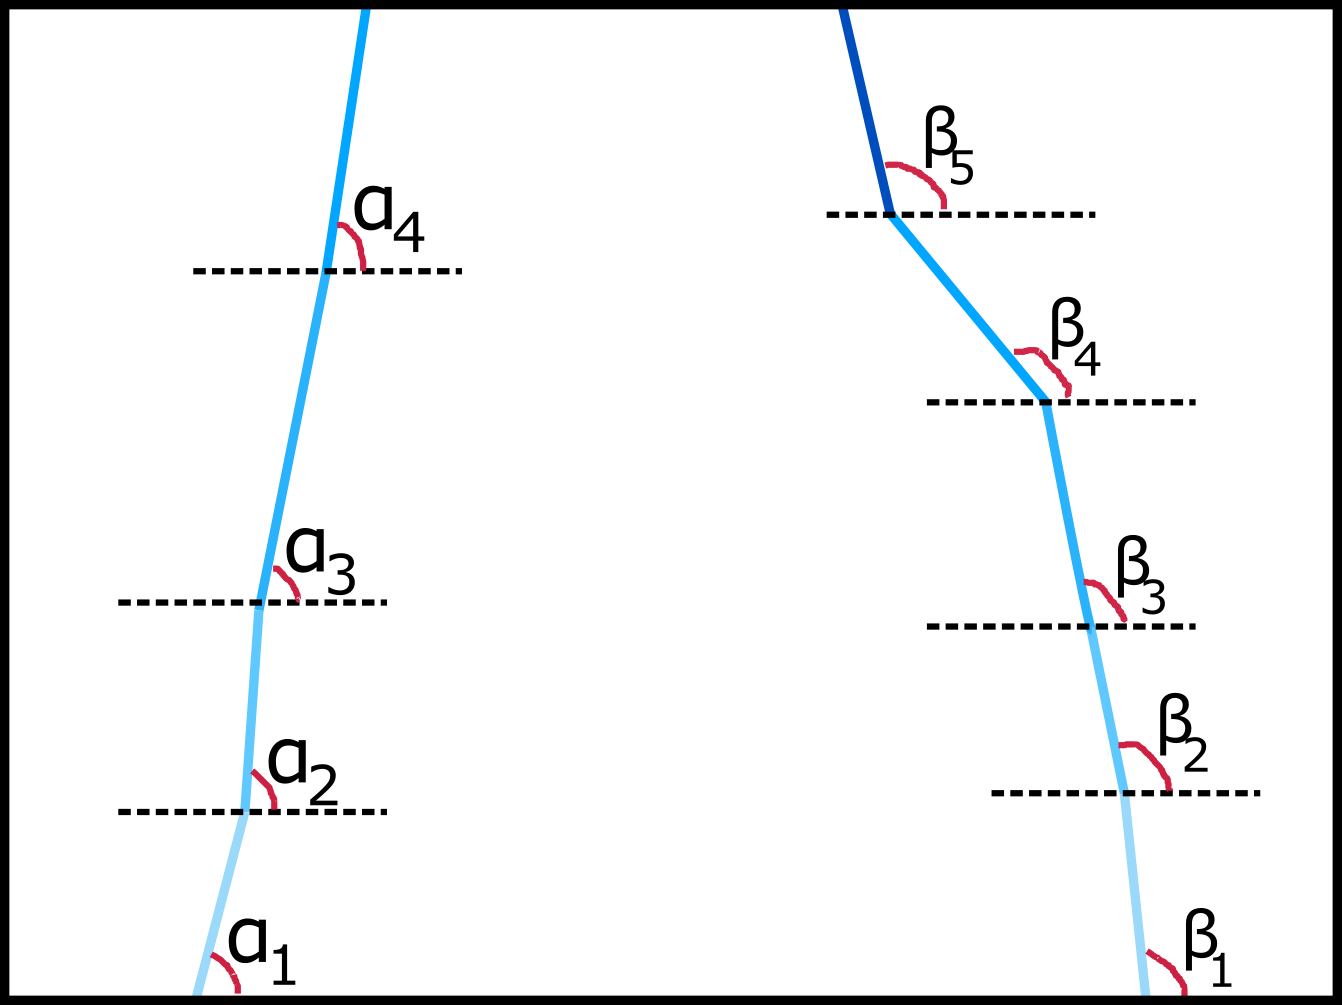
\includegraphics[width=0.44\unitlength]{images/dataP_explained3}

\caption{\label{fig:dataP_explained3} Before Eliminating Incorrect Lines}

\end{subfigure}%
\begin{subfigure}{.46\textwidth}

\centering

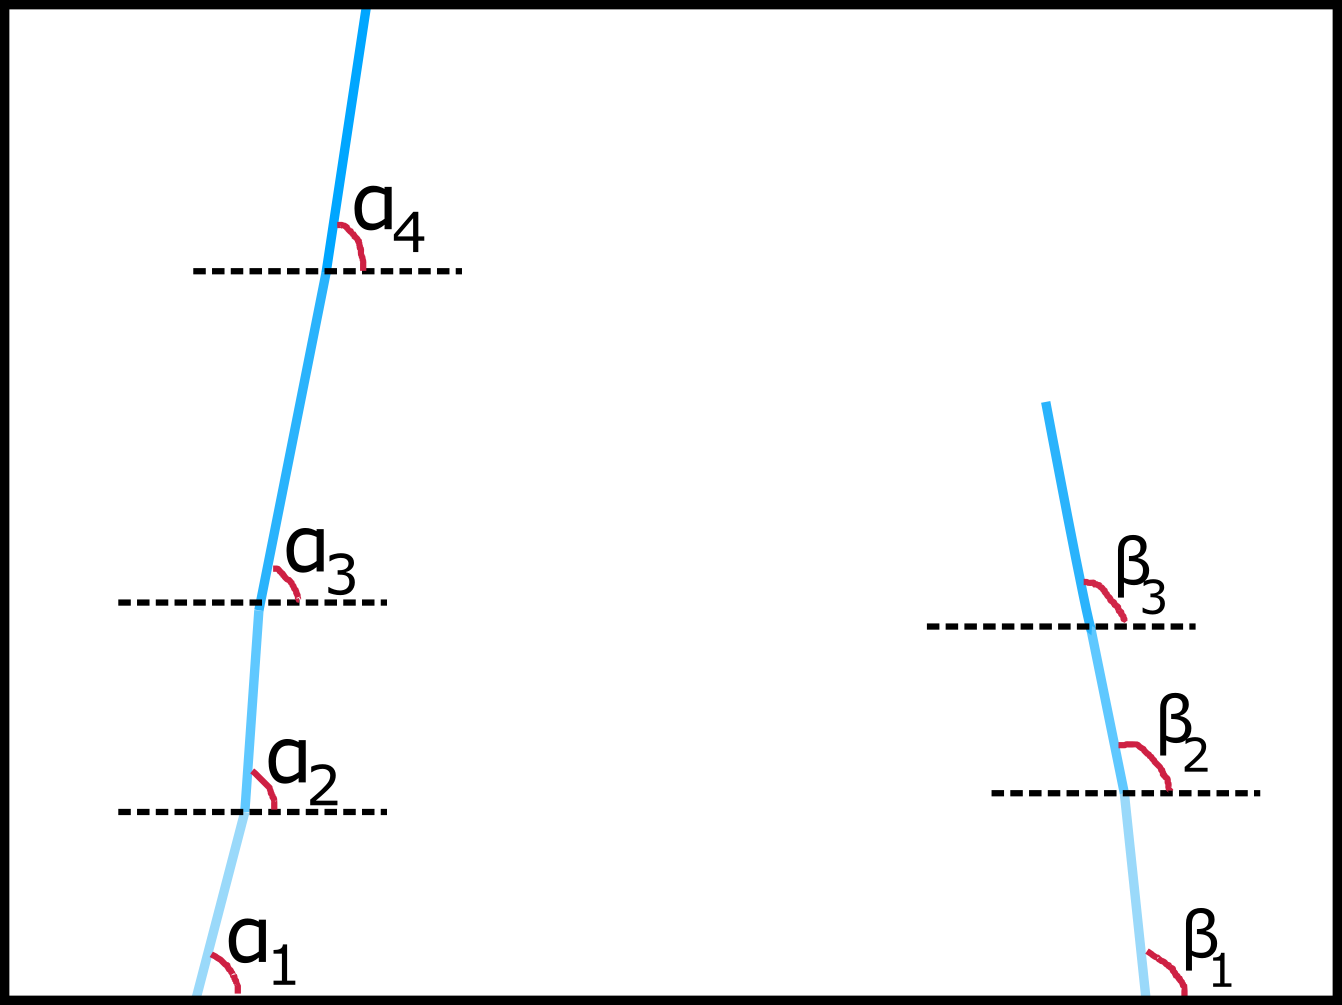
\includegraphics[width=0.44\unitlength]{images/dataP_explained4}

\caption{\label{fig:dataP_explained4} After Eliminating Incorrect Lines}

\end{subfigure}

\caption{\label{fig:dataP_explainedBroken} Another Scenario on Eliminating Incorrect Lines}

\end{figure}

The third step is to fit best lines through the remaining lines. This is realized by using built-in Least-Squares method. As a result of this step, the number of lines is dropped to two as left line and right line.


The last step is to find the steering angle. The target point is determined as the average of the middle points left and right lines. So the target point is always in the form of $(x_{avg}, 305)$. The y-coordinate is found by simple math (referencing from \textit{Figure~\ref{fig:camera_vision_explained}}) $480px-50px-125px$. The current point of the vehicle is always $(320,480)$. So the line connecting two points to each other constitutes the track path and the $arctan$ of the slope gives the steering angle. Steering angle is in the $[-90,90]$ range where negative values indicate to turn left and positive values indicate to turn right. This output is sent to PID Controller subsystem.
\begin{algorithm}[t]
	
	
	
	\DontPrintSemicolon
	
	
	$array[n] lines $\;
	
	$array[n] line\_slope\_angles $\;
	
	$array[n-1] slope\_angle\_differences$ \;
	
	
	$slopeAngle\_threshold $\;
	
	$slopeAngle\_difference\_threshold$ \;
	
	
	%	\KwData{Testing set $x$}
	
	\For{slope\_angle\_differences}{ 
		
		\If{$k$th item $>$ slopeAngle\_difference\_threshold}{
			
			// Check $k$th and $(k+1)$th items in line\_slope\_angles array
			
			
			\If{$k$th item in line\_slope\_angles array $>$	slopeAngle\_threshold}{
				
				Mark index $k$ in lines array problematic
				
			}	
			
			\ElseIf{$(k+1)$th item in line\_slope\_angles array $>$	slopeAngle\_threshold}{
				
				Mark index $(k+1)$ in lines array problematic
				
			}	
			
		}
		
	}
	
	Delete the lines between problematic indexes 
	
	\caption{Line Elimination Algorithm}
	
	\label{algo:eliminateLines}
\end{algorithm}


\item {Discussions on the Solution}


The proposed algorithm is mostly the same as in Conceptual Design Review Report. An improvement is made on the way algorithm determines the center of the image. With this new approach, image center is always determined correctly. Line classification and obstacle elimination show satisfactory results regarding robustness.

\end{enumerate}


%%%%%%%%%%%%%%%%%%%%%%%%%%%

\newpage

\subsubsection{PID Controller Subsystem}\label{sect:ControllerSubsystem}

\begin{enumerate}
	\item {Requirements for the Solution}
	
	\begin{enumerate}
		\item The subsystem should be able to control the motors
		\item The subsystem should be able to react the external disturbances
	\end{enumerate} 
	
	
	\item {Solution for the Subsystem}
	
	
	\textit{PID Controller Subsection} is the main subsystem of the vehicle whose reponsibility is keeping the vehicle at the middle of the path it is following. To achieve this task, this subsystem includes a PID controller for the lateral movement of the vehicle. As the achieved purpose is to stay in the middle of the lane, this subsystem creates a PWM differences between motors in order to rotate the vehicle via differential drive. 
	
	
	For that purpose, the \textit{Data Processing Subsystem} produces the necessary feedback elements for this subsystem. For the control purpose, in ideal circumstances data processing unit determines eight main point on its vision to create processed variables as in \textit{Figure~\ref{fig:controlled-vars}}. These can be explained namely as;
	
	\begin{itemize}
		\item \textbf{A1 \& A2:} Beginning and end points of left line at ROT (Region of Target).
		\item \textbf{B1 \& B2:} Beginning and end points of right line at ROT.	
		\item \textbf{Image Center Back (ICB):} Beginning point of our heading line in ROT.
		\item \textbf{Image Center Front (ICF):} End point of our heading line in ROT.  
		\item \textbf{Lane Center Back (LCB):} The middle point of the lane at the starting of the ROT. Can be found by averaging $A1$ $\&$ $B1$.
		\item \textbf{Lane Center Front (LCF):} The middle point of the lane at the end of the ROT. Can be found by averaging $A2$ $\&$ $B2$.
	\end{itemize}	   
	
	
	%%%%%%%%%%%%%%%%%%%%%%%%%%%
	
	
	\begin{figure}[H]
		\setlength{\unitlength}{\textwidth} 
		\centering
		\begin{subfigure}{.46\textwidth}
			\centering
			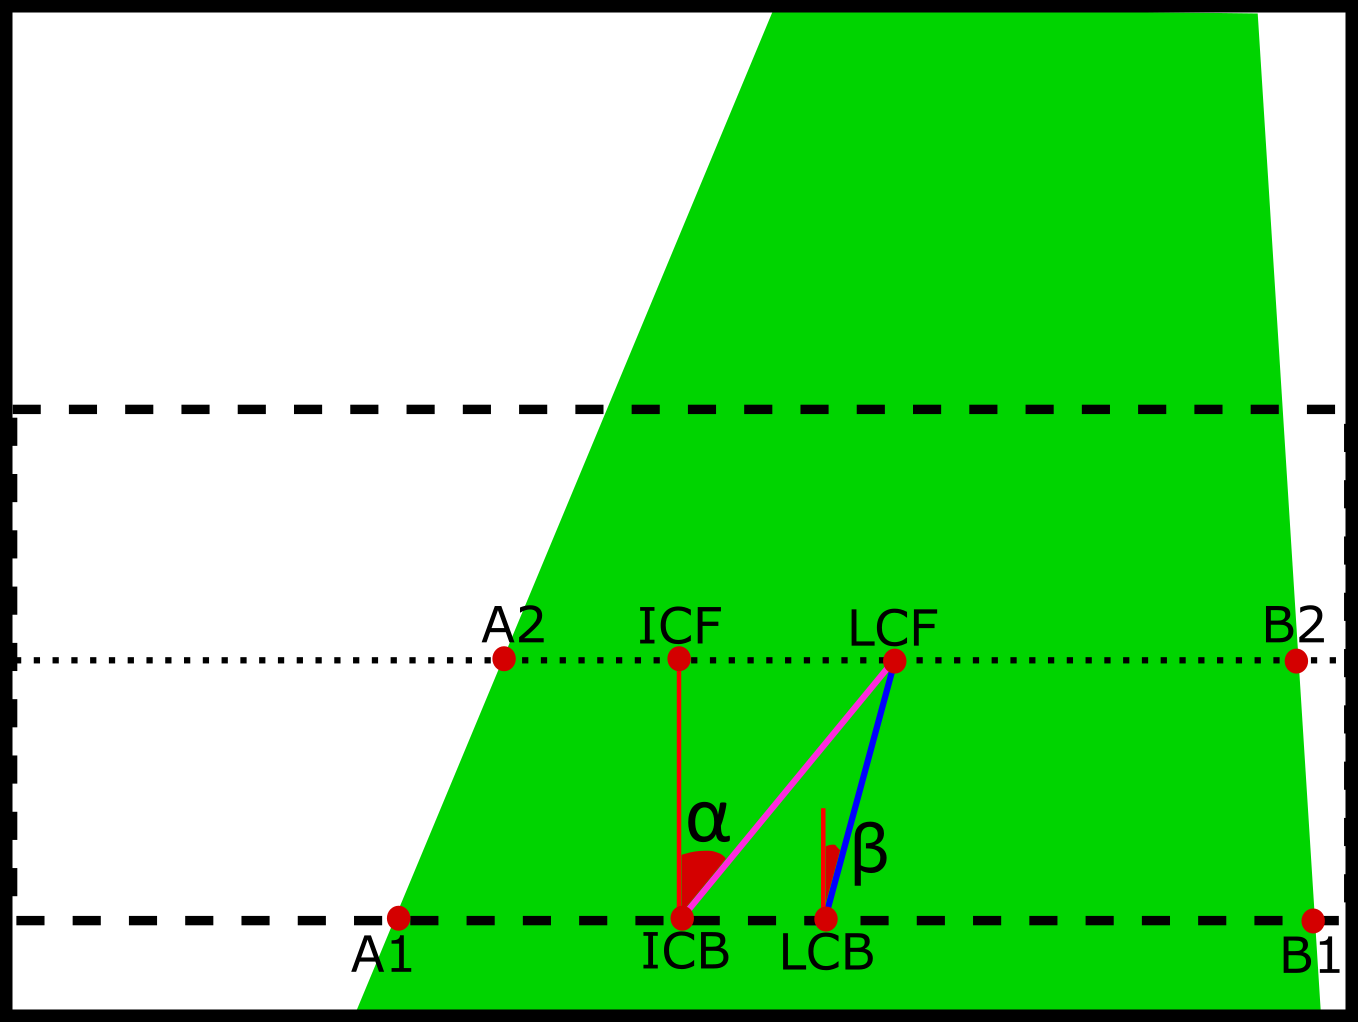
\includegraphics[width=0.45\unitlength]{images/ang_cont}
			\caption{\label{fig:ang-cont} Controllable Angle Variables }
		\end{subfigure}%
		\begin{subfigure}{.46\textwidth}
			\centering
			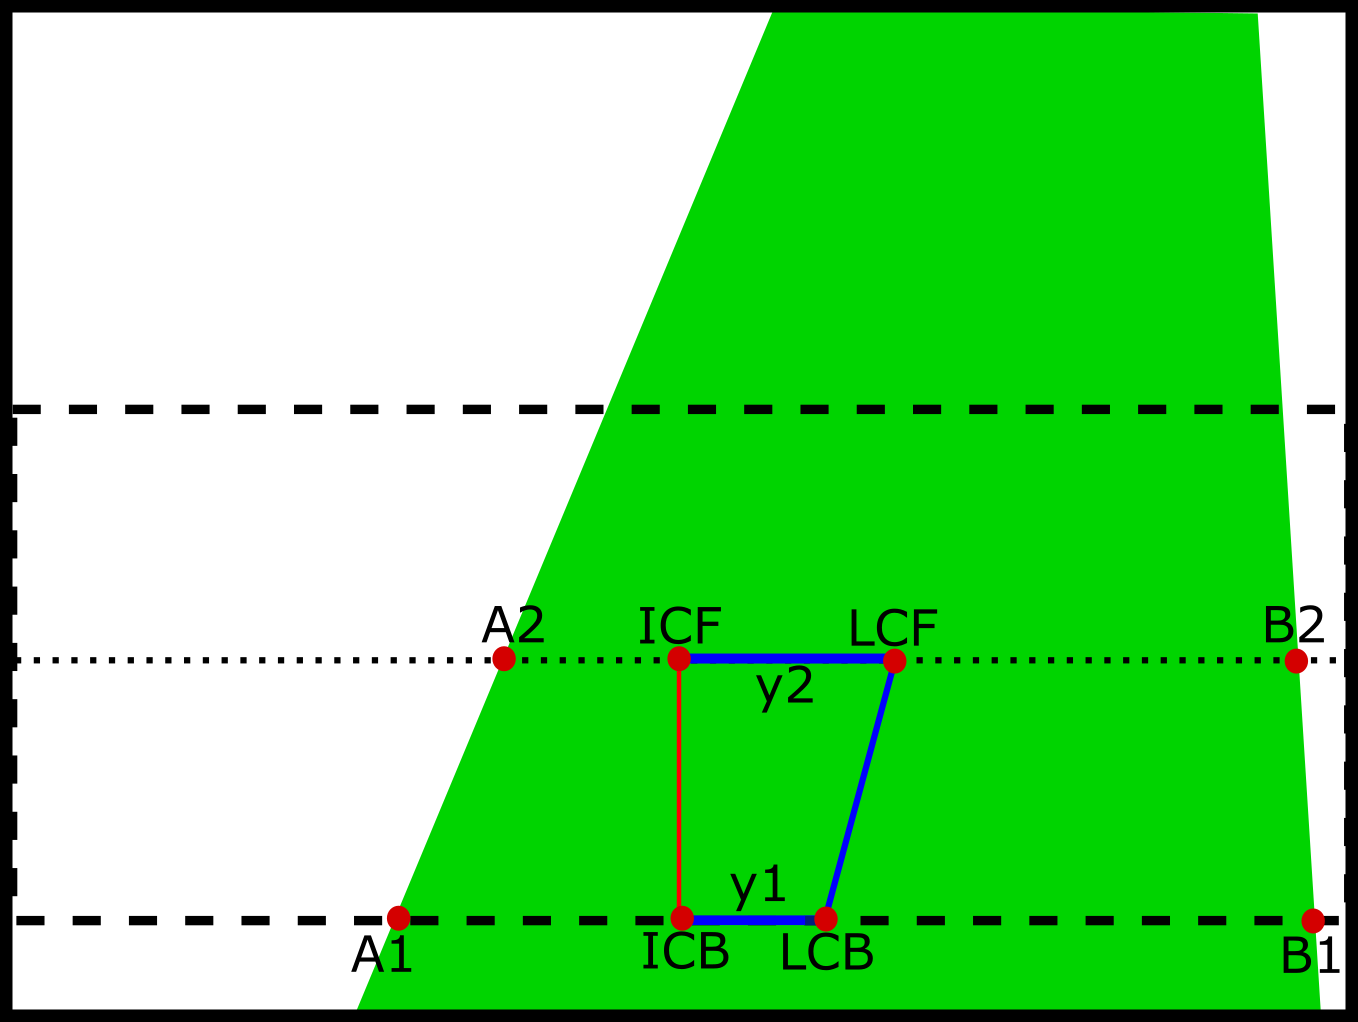
\includegraphics[width=0.45\unitlength]{images/dist_cont}
			\caption{\label{fig:dist-cont} Controllable Distance Variables}
		\end{subfigure}
		\caption{\label{fig:controlled-vars} Controlled Variables of the System }
	\end{figure}
	
	
	%%%%%%%%%%%%%%%%%%%%%%%%%%%
	
	
	By utilizing these points and their coordinates, the data processing can produce four main variables that can bee used for PID controller and speed subsystems. These are;
	
	\begin{itemize}
		\item \textbf{$\alpha$:} The angle between the current direction of the vehicle and the direction the vehicle should follow in order to arrive at point \textbf{LCF}. It is a main controlled variable for lateral position control with angle variable.
		\item \textbf{$\beta$:} The angle of the line that connects the points \textbf{LCB} and \textbf{LCF}. It represents the angle of the lane, and it can be used for longitudinal movement control in speed subsystem.
		\item \textbf{y1:} The instantaneous distance error of the vehicle from the center line. It can be calculated by subtracting the x-coordinate of \textbf{LCB} from the x-coordinate of \textbf{ICB}. Due to delays in the system, it is not fed to controller. However, it is a quite useful variable for observing the system.  
		\item \textbf{y2:} The expected distance error of the vehicle from the center line at the end of ROT. It can be calculated by subtracting the x-coordinate of \textbf{LCF} from the x-coordinate of \textbf{ICF}. This results in a distance in a scale of pixels, to convert this to a distance in centimeter, the error can be multiplies by a constant. It is a main controlled variable for lateral position control with distance variable.
	\end{itemize}	 			
	
	
	
	In our application, we have decided to use distance variable $y_1$ and angle variable for control purposes. The main pupose of the PID Subsystem is to compansate the lateral distance error of the vehicle, i.e., staying exactly on the center lane. In our control design, we have descided to use $y_1$ as control signal and, zero as reference signal. Basic block diagram can be seen at \textit{Figure~\ref{fig:blockdiagram}}. The output of this PID controller then send to the DC motors as PWM difference. The actual base PWM is produced by the Speed Subsystem.
	
	
	\begin{figure}[h]
		\includegraphics[width=\textwidth,center]{images/Simulink/Block_Diagram}
		\caption{Block Diagram of the Project and the Interaction of the Subsystems}\label{fig:blockdiagram}
	\end{figure}
	
	
	
	%\subsubsection*{Modelling the Plant}
	
	%Modelling a plant is a good practice in controller design applications, however, in our case the model for the vehicle is unstable, thus applying a bump test as in \textit{Figure~\ref{fig:bump2}} results with a exponentially increasing processed data 'y2'. Thus, in this project, our aim is to apply bump test to closed loop system as in \textit{Figure~\ref{fig:bump1}} with a known P-controller. An approximate plant model from there can be found as follows;
	
	%$$ T(s)=\frac{G_c(s)G_p(s)}{1+G_c(s)G_p(s)} $$
	
	%If the overall step response can be modelled resulting with $T(s)$
	
	%$$\boxed{ G_p(s)=\frac{T(s)}{G_c(s)-T(s)G_c(s)} }$$ 
	
	%Using this plant model, parameters for PID controller can be designed using \textit{Matlab Simulink}.
	
	
	%\begin{figure}[h]
	%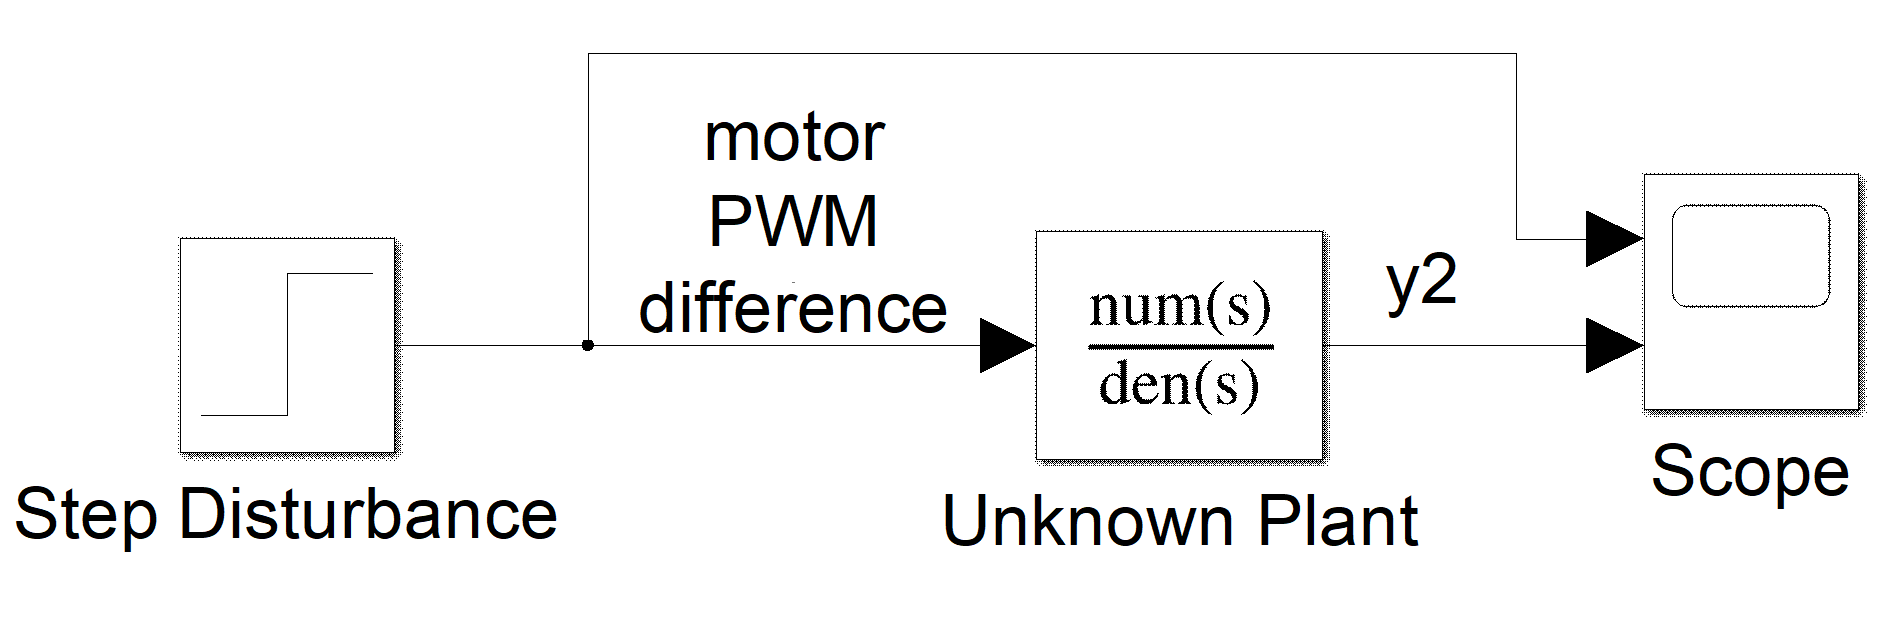
\includegraphics[width=0.75\textwidth,center]{images/simulink/modelling2}
	%\caption{Bump Test for the Unknown Plant \label{fig:bump2} }
	%\end{figure}
	
	%\begin{figure}[h]
	%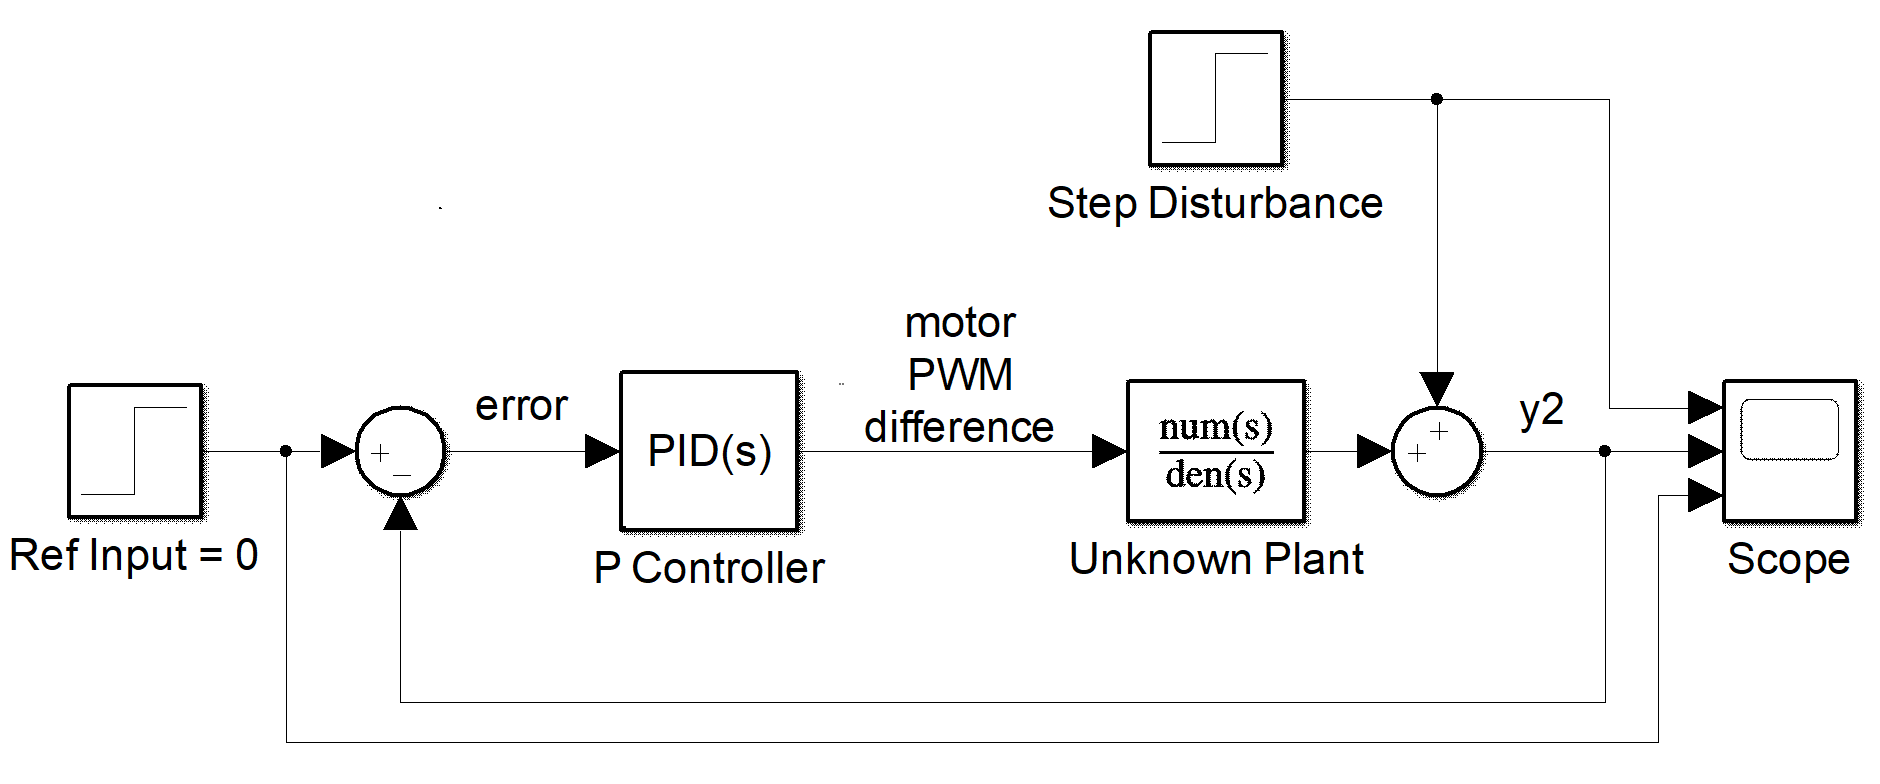
\includegraphics[width=1\textwidth,center]{images/simulink/modelling1}
	%\caption{Bump Test for the Closed Loop System \label{fig:bump1} }
	%\end{figure}
	
	\subsubsection*{ Pulse Transfer Function of a Digital PID Controller }
	
	However, since the controller operates on the microcontroller, therby, on discrete-time domain. We firstly find its pulse transfer function and transferred it to discrete-time domain. General PID controller can be expressed in \textit{Laplace} domain as 
	
	
	$$ G_c(s)=K_c(1+\frac{1}{\tau_I s}+\tau_d s )$$  
	
	
	\paragraph*{ Discritization of I Controller }
	
	Casual discrete time approximation of the I-Controller can be written as;
	
	$$  y[k]=y[k-1]+\frac{u[k]+u[k-1]}{2}*T_s $$
	
	Where $y[k]$ is output and $u[k]$ is the output. Taking its Z-transform, the pulse transfer function becomes,
	
	$$ Y(z) = Y(z) z^{-1}=\frac{T_s}{2}\left(U(z)+U(z)*z^{-1} \right) $$
	
	$$ G_I(z)=\frac{Y(z)}{U(z)}=\frac{T_s (1+Z^{-1})}{2 (1+Z^{-1})} $$
	
	\paragraph*{ Discritization of D Controller }
	
	Casual discrete time approximation of the D-Controller can be written as;
	
	$$  y[k]=\frac{e[k]-e[k-1]}{T_s} $$
	
	Where $y[k]$ is output and $e[k]$ is the error input. Taking its Z-transform, the pulse transfer function becomes,
	
	$$ Y(z) = Y(z) z^{-1}=\frac{T_s}{2}\left(E(z)+E(z) z^{-1} \right) $$
	
	$$ G_D(z)=\frac{Y(z)}{E(z)}=\frac{(1-Z^{-1})}{T_s} $$
	
	
	Therefore pulse transfer function of the PID controller becomes,
	
	$$ G_{PID}(z)=K_p+	\frac{T_s (1+Z^{-1})}{2 (1+Z^{-1})} + \frac{(1-Z^{-1})}{T_s} $$
	
	$$ \boxed{	 G_{PID}(z)=\cfrac{K_p(1-z^{1})+K_i \frac{T_s (1+z^{-1})}{2}+K_d (1-2z^{-1}+z^{-2})}{1-z^{-1}}	}$$	
	
	\subsubsection*{Implementation of the PID Controller}
	
	$$ \frac{Y(z)}{E(z)}=\frac{K_p(1-z^{1})+K_i \cfrac{T_s (1+z^{-1})}{2}+\cfrac{K_d}{T_s} (1-2z^{-1}+z^{-2})}{1-z^{-1}}$$
	$$ Y(z)-z^{-1} Y(z)=K_p E(z)-K_p z^{-1} E(z)+\frac{K_i T_s}{2} E(z) +\frac{K_i T_s}{2} E(Z) z^{-1} .. $$
	$$ +\cfrac{K_d}{T_s} E(z)-2 z^{-1} E(z)+\cfrac{K_d}{T_s} z^{-2} E(z)	$$
	$$ y[k]-y[k-1]=K_p e[k]-K_p e[k-1]+\frac{K_i T_s}{2}+K_i T_s e[k-1]/2+\cfrac{K_d}{T_s} e[k]-2 e[k-1] \cfrac{K_d}{T_s}+ \cfrac{K_d}{T_s} e[k-2]	$$
	$$ y[k]-y[k-1] = (K_p+\frac{K_i T_s}{2}+K_d) e[k]+(-K_p+\frac{K_i T_s}{2}-2 \cfrac{K_d}{T_s} ) e[k-1]+(\cfrac{K_d}{T_s}) e[k-2] $$
	
	If we add all past terms together to find $y[k]$,
	
	\begin{align*}
	y[k]-y[k-1] = (K_p+\frac{K_i T_s}{2}+\cfrac{K_d}{T_s})&e[k]+(-K_p+\frac{K_i T_s}{2}-2 \cfrac{K_d}{T_s})e[k-1]..\\
	+(K_d)&e[k-2]\\
	y[k-1]-y[k-2] = (K_p+\frac{K_i T_s}{2}+\cfrac{K_d}{T_s})&e[k-1]+(-K_p+\frac{K_i T_s}{2}-2 \cfrac{K_d}{T_s})e[k-2]..\\
	+(K_d)&e[k-3] \\
	y[k-2]-y[k-1] = (K_p+\frac{K_i T_s}{2}+\cfrac{K_d}{T_s})&e[k-2]+(-K_p+\frac{K_i T_s}{2}-2 \cfrac{K_d}{T_s})e[k-3]..\\
	+(K_d)&e[k-4]\\
	...\\
	...\\
	y[k-n]-y[k-n-1] = (K_p+\frac{K_i T_s}{2}+\cfrac{K_d}{T_s})&e[k-n]+(-K_p+\frac{K_i T_s}{2}-2 \cfrac{K_d}{T_s})e[k-n-1]..\\
	+(K_d)&e[k-n-2]\\
	y[k]-y[k-n-1]= (K_p+\frac{K_i T_s}{2}+\cfrac{K_d}{T_s})&e[k] + (K_i T_s-\cfrac{K_d}{T_s})e[k-1] + (K_i T_s)e[k-2] ..\\ 
	+ (K_i T_s)&e[k-2]  .... +  (K_i T_s)e[k-n-1]
	\end{align*}
	
	Therefore;
	
	$$ 	\boxed{ y[k] = y[k-n-1]  + K_p (e[k] ) + K_d ( \frac{e[k]-e[k-1] }{T_s} )  + K_i (T_s  	 \sum_{i=0}^{n+1} e[k-i])  } $$
	
	This equation was utilized on Arduino microcontroller considering the past three errors for the integral term.
	
	
	
	\paragraph*{Sampling Time Matching and Controller Output Limit}
	
	In our implementation, the sampling time of the plant, i.e., the processing time in which the Raspberry Pi processes each picture frame is approximately 54 miliseconds, however, the sampling time of each Arduino loop is very small in comparison to our sampling time. To handle this proplem, we implemented delay function of the Arduino to match the sampling times.
	
	A saturation limit is also present to keep the overall PWM signal send to the DC motors within a 0-255 PWM range to prevent oscillation. Another saturation limit also controls the output of the controller subsystem to avoid any undesired errors that might happen at the video processing.
	
	Overall PID algorithm can be investigated at \textit{Algoritm~\ref{algo:PID}}.
	
	\begin{algorithm}
		\DontPrintSemicolon	
		maxSum // Integral Wind-up term \\
		Ts // Sampling time \\
		// Update of past error array \\
		\For { int i = (pastSize - 1) $\to$ 0 } {
			pastError[i] = pastError[i - 1] 
		} 
		pastError[0] = error \\
		// Calculation of Derivative Term \\
		delta = (pastError[0] - pastError[1]) / Ts \\
		// Calculation of Integral term \\
		sum = sum + (pastError[0] + pastError[1] + pastError[2]) / 3 * Ts \\
		sum = min(max(sum , -1 * maxSum), maxSum) // Anti-Wind-up  \\
		// Calculation of PID output \\
		motorCmd = int(Kp * error + Kd * delta + Ki * sum)	\\	
		motorCmd =  min(motorCmd,Max\_Delta\_PWM) \\
		delay(Ts-duration) // duration:duration of each Arduino loop	
		\caption{PID Controller Algorithm}
		\label{algo:PID}
	\end{algorithm}
	
	\paragraph*{Classification of Path Rotation}
	
	Due to unidealities of the motors, the controller tuned for the CCW movement failed to pass the test proposed under \textit{Section~4.4}, therefore, the PID parameters and the base speed parameters were seperated in order to have same performance at both sides. 
	
	It should be also noted that, the \textit{Data Processing Subsystem} produces $\beta$ in $0-180$ degree range if the path is located with a positive angle with respect to vehicle or produces $\beta$ in $180-360$ degree range otherwise.
	In that notation sense, if the $\beta$ is in $0-180$ degree range the vehicle is being operated on a path at counterclockwise direction and at clockwise diirection if the $\beta$ is in $180-360$ degree range.
	
	However, since the main frame of the video input, i.e., orientation of the vehicle is moving constantly, the counterclockwise movement can be understood by the vehicle if an undesired input changes the direction of the vehicle dramatically. To avoid these undesired effect on the controller and base speed calculation, an array that holds past five angle information was created. At every frame, the angle classified as $1$ or $0$ according to its degree range. The purpose of this array is to elliminate the undesired rotation determination array by checking last five angle data. The basic algoithm can be further investigated at \textit{Algorithm~\ref{algo:rotation}}. 
	
	According to the value of \textit{yonFin} variable, PID parameters tuned for both direction is fed to the controller algorithm.
	
	\begin{algorithm}
		\DontPrintSemicolon	
		pastYon[yonSize] // Holds past rotations, has elements 0 or 1 \\
		// Update pastYon array \\ 
		\For {int i = (yonSize - 1) $\to$  0} {
			pastyon[i] = pastyon[i - 1]
		}
		$ pastyon[0]=yon $\\
		yonSum $=$ 0 \\
		\For {int k $=$ 0  $\to$ (yonSize-1) }
		{
			$ yonSum = yonSum + pastyon[k] $
		}
		$ yonAvg=yonSum/yonSize $\\ 
		\If { yonAvg  $<$  0.5} {
			$yonFin=0$ 
		}   
		\Else {
			$yonFin=1$ 
		}
		\caption{Path Rotation Classification Algorithm}
		\label{algo:ratation}
	\end{algorithm}
	
	\item {Discussions on the Solution}
	
	The proposed algorithm lacks the modelling of the system, thus, tuning of the PID parameters were handled by try and error. The state-space model of the plant will further be investigated under the term project of the another undergraduate course of our department, EE498:CONTROL SYSTEM DESIGN AND SIMULATION. However, it was not included due to its incompleteness.	
	
	Other than the modelling part and rotation sensitivity, the proposed methods are same as the ones proposed in the conceptual design review report. And they function as expected. 


\end{enumerate}

%%%%%%%%%%%%%%%%%%%%%%%%%%%	

\subsection{Communication System}


	%This systems is responsible for all communication responsibility of the system. It is one of the most crucial systems of this project since it is responsible for safe communication between subsystems with each other. It is also responsible for communication with other vehicles.	And the requirements for this system are as follows;		

	\begin{enumerate}
		\item The subsystem should ensure safe internal communication
		\item The subsystem should ensure safe external communication
	\end{enumerate}	


	The system has two subsystems namely, 	,

	\begin{enumerate}
		\item \textbf{Internal Communication Subsystem} which is responsible for communication inside the vehicle mainly the communication between Raspberry Pi and Arduino.						
		\item \textbf{External Communication Subsystem} which is responsible for the communication of the vehicle with the outside world mainly with the opponents.
	\end{enumerate}		

%%%%%%%%%%%%%%%%%%%%%%%%%%%	

\subsubsection{Internal Communication Subsystem}


	\begin{enumerate}
		\item {Requirements for the Solution}
		
		\begin{enumerate}
			\item The microcontrollers should be able to communicate with each other via serial communication
			\item The internal communication speed should be compatible with the processing speed of the lane detection subsystem  
		\end{enumerate}
	
	\item {Solution for the Subsystem}

		%This subsystem covers the communication of the components inside vehicle. Currently, Raspberry Pi and Arduino are two components that requires communication. To prevent the large amount of cable connection, a serial communication protocol is implemented. \\
		
		%The serial communication is implemented via USB port. Since RPi is practically a computer, it can recognize Arduino as a device using a serial port such as \lstinline|/ttyUSB0| in case of a Linux based OS. When recognized, RPi can send any piece of strings to the Arduino via USB cable. The process of communication is as follows:

	\begin{enumerate}
		\item Arduino should be connected to the Pi. \vspace{-0.2cm}
		\item Using Arduino IDE or any other method such as listing serial ports and checking for Arduino and so on, the serial port name should be detected \vspace{-0.2cm}
		\item Baud rates of two sides should be the same. 9600 is generally enough but if needed, it can be incremented to satisfy fast communication rate. \vspace{-0.2cm}
		\item On Arduino side, \texttt{Serial.begin(9600)} command should be executed and serial port should be read repeatedly to capture the incoming data \vspace{-0.2cm}
		\item On Pi side, using  C++ messages can be send to serial port
\end{enumerate}

	%Since the lane detection algorithm is implemented on C++, serial communication on the Raspberry side is also implemented on C++. Using \lstinline[language=C++]|<wiringPi.h>| and \lstinline[language=C++]|<wiringSerial.h>| libraries any string can be sent to the serial port specified by the string \lstinline[language=C++]|/dev/ttyACM0"| with a specified baud rate. 


\begin{lstlisting}[language=C++,caption={C++ class for serial communication}]
void ArduinoComm::sendToController(std::string payload) {
/*************************/
int serialDeviceId = 0;
serialDeviceId = serialOpen("/dev/ttyACM0", 9600);
std::cout << "sender " << serialDeviceId << std::endl;
if (serialDeviceId == -1) {
std::cout << "Unable to open serial device" << std::endl;
return;
}
if (wiringPiSetup() == -1) {
return;
}
serialPuts(serialDeviceId, payload.c_str());
return;
}
\end{lstlisting}

	%On the Arduino side, the commands coming from serial port should be listened. The preferred way of achieving that task is to use \texttt{SerialCommand.h} library for the Arduino which allows executing a function depending on the incoming string. Using \lstinline|.addCommand("str",func)| function of the library any function \textit{\lstinline|func|} can be associated with any string coming from serial port. Moreover, the functions can have argument. For example, let the string "PWMSET" be execute a function \lstinline|setpwm()| which requires the PWM value as argument. If incoming string is of the form "PWMSET 150", using \lstinline|.next()| function of the library, the value 150 can be read and converted into integer and interpreted as the PWM value to be set by the function.\\

	\item {Discussions on the Solution}

		%Using that library, consecutive commands with less that 1ms time separation are sent and the reliability of the library is tested. The results are positive. Since the lane detection algorithm is generating angle and position data approximately in every 7ms, the performance of the library is more than enough for this purpose.			

	\end{enumerate}


%%%%%%%%%%%%%%%%%%%%%%%%%%%
%%%%%%%%%%%%%%%%%%%%%%%%%%%


\subsubsection{External Communication Subsystem}	



\begin{enumerate}
	\item {Requirements for the Solution}
	
	\begin{enumerate}
		\item The subsystem should be able to communicate with the opponent via P2P Wi-Fi protocol
		\item The subsystem should start race with the 3-way handshake mechanism required for establishment of TCP connection
		\item Similarly, the subsystem should be able to trigger similar handshake mechanism during the race, which is referred as the main handshake mechanism throughout this report
		\item For the second handshaking, the subsystem should be able to get the sensor data from vehicle detection subsystem to send messages
		\item LEDs with corresponding colors should be lid to identify and display the messages that are sent
		
	\end{enumerate}
	
	\item {Solution for the Subsystem}
	
	\begin{figure}[h]
		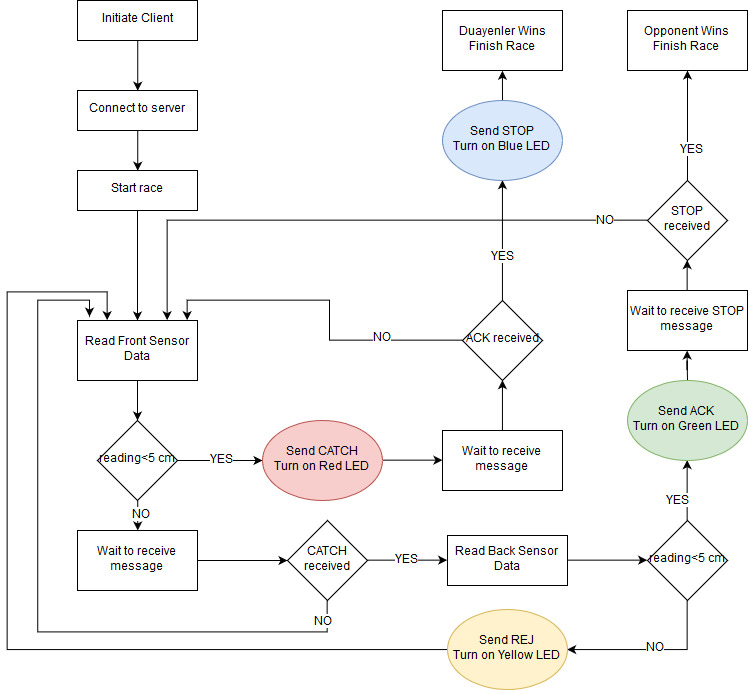
\includegraphics[width=0.8\textwidth,center]{images/client_asm}
		\caption{ASM Chart of the Algorithm of the External Communication Subsystem for Client Side \label{fig:asmclient} }
	\end{figure}
	
	\begin{figure}[h]
		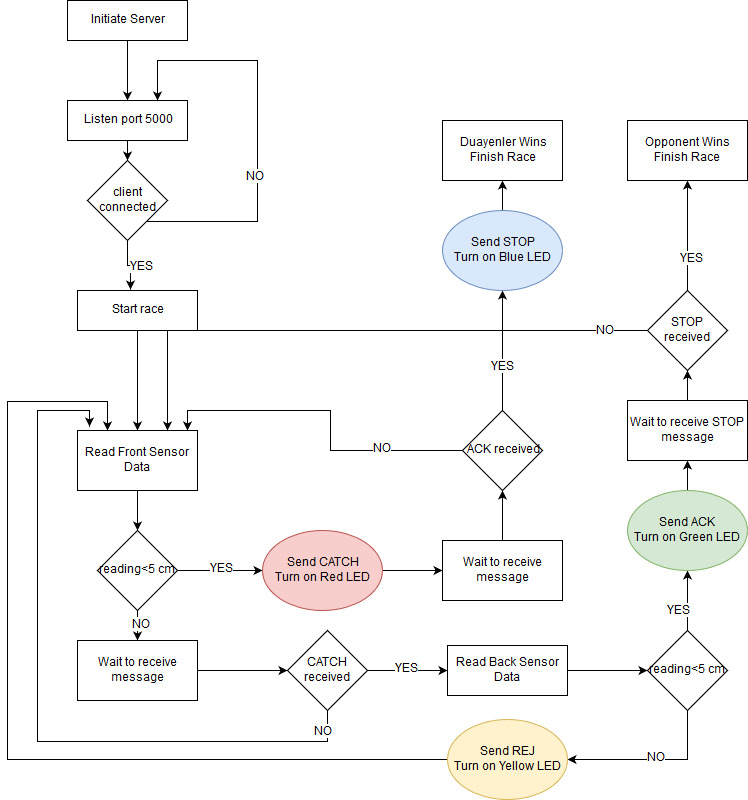
\includegraphics[width=0.8\textwidth,center]{images/server_asm}
		\caption{ASM Chart of the Algorithm of the External Communication Subsystem for Server Side \label{fig:asmserver} }
	\end{figure}
	
	The main solution for this subsystem is setting the device as a P2P host. Sockets are used to send or receive messages.  Since the host can act as a server as well as a client, both socket functions are used to establish communication. The subsystem requires opponent ID and host type(client/server) from the user and sensor readings from the vehicle detection subsystem. It can initiate and terminate other subsystems when necessary.
	
	The first step of the game is setting up a Wireless Ad-Hoc Network. The fact that which side will provide the network is decided according to the the agreement with the opponent. After that decision, by changing the Pi's configuration files accordingly, one side sets up the network and the other connects to it after rebooting.
	
	To implement the communication, the socket data structures are created in both server and client sides. At the beginning of the race, the peer acting as a server listens to the port 5000, which is specified in Standard Committee. Then, the connect() function is called in the client side, so that the request is sent. At the same time, server side acknowledges the request by means of accept() function. At this moment, client side also sends acknowledgement by default, hence race starts. The peers are connected during the race. This mechanism is common in every protocol that utilizes TCP, and called 3-way handshake.
	
	The process for the finishing handshake also utilizes socket functions, but the process is a little bit different. For the win case, vehicle detection subsystem (front sensor) initiates the handshake. A catch message (ID00) is sent to the opponent. If acknowledgment is taken from the opponent, stop message (ID10) is sent. On the other hand, for the defeat case, a catch message is received by the opponent. Then, vehicle detection subsystem is called. According to the returned value from the back sensor, the acknowledge (ID01) or reject (ID11) are sent. Also, LEDs corresponding to messages are lid for the finishing handshake.
	
	
	
	The ASM chart describing the algorithm of the external communication subsystem can be seen in \textit{Figure~\ref{fig:asmserver}} and \textit{Figure~\ref{fig:asmclient}}, for client and server sides, respectively. The fact that which team will be server or client is decided with the agreement between the teams before the race. Notice that, the only difference between client and server codes is the TCP connection parts before starting the race. 
	
	In the simplest form, there are two repeated actions inside the main loop. Firstly, front sensor is read. Secondly, device waits to receive message before timeout occurs. Setting proper timeout value is a little bit tricky. It is done according to the tests conducted with the opponents. The details of it can be found in the "External Communication Subsystem Tests and Results" section.
	
	
	\item {Discussions on the Solution}
	
	The proposed method is not changed after the Critical Design Review Report. In the previous report, creating an ad-hoc wifi is proposed, but was not implemented. Implementation has been done by making appropriate changes in Pi's configuration files. The code was previously written in Python for simplicity. To unite it with image pocessing code, it is rewritten in C++. Besides, improvements such as adding proper timeout value and LED integration is made.
\end{enumerate}




\subsection{Driving System}

	%This system is responsible for the motion of the vehicle. Two parameters that are the direction and the speed of the vehicle is controlled by this unit accordingly to the information coming from the \textit{Computation System}. And the requirement for this system are as follows;


	\begin{enumerate}
		\item The subsystem should control motion subsystem according to output of the computation system		
	\end{enumerate}

	The system has two subsystems namely,
		
	\begin{enumerate}
		\item \textbf{Direction Subsystem} which is responsible for the orientation of the vehicle and keeps the road and the vehicle aligned.
		\item \textbf{Speed Subsystem} which is responsible for the overall speed of the vehicle by adjusting it considering other effects on the vehicle.
	\end{enumerate}


\subsubsection{Direction Subsystem}

	\begin{enumerate}
		\item {Requirements for the Solution}
		
		\begin{enumerate}
			\item The subsystem should drive the motors according to computation system outputs
			\item The system should ensure that the vehicle follows the lane 	
		\end{enumerate}

		\item {Solution for the Subsystem}

		%As will be explained in more detail in \textit{Structure System}, the vehicle has two DC motors and one caster-ball as a movement part. This subsystem uses differential drive in order to drive the vehicle. This subsystem will get two important parameter from other subsystems, namely;

		\begin{itemize}
			\item PWM Offset Value that determines the speed of the vehicle at longitudinal movement. This data is acquired from the \textbf{Speed Subsystem.} 	
			\item PWM Difference Value that determines the speed difference between the two motors. This difference helps the vehicle in lateral movement. This data is acquired from the \textbf{PID Controller Subsystem.} 	
		\end{itemize}	


	%H-bridge motor drivers are used to drive DC motors. L298N motor driver with voltage regulator is used for this purpose in this project. 


	\item {Discussions on the Solution}

		%The solution for this subsystem is a very similar solution as discussed in \textit{Conceptual Design Report}. Since we performed the test for this subsystem even before the conceptual design stage and they were satisfying technical requirements, the solution was not altered. 

	\end{enumerate}


%%%%%%%%%%%%%%%%%%%%%%%%%%%

\subsubsection{Speed Subsystem}

\begin{enumerate}
	\item {Requirements for the Solution}
	
	\begin{enumerate}
		\item The subsystem should decrease the vehicle speed at the narrow lane 
		\item The subsystem should increase the vehicle speed at the wide lane
		\item The subsystem should decrease the vehicle speed at the extreme disturbance  
	\end{enumerate}
	
	\item {Solution for the Subsystem}
	
	This subsystem is responsible for determining the base speed of the both DC motors. In order to do so, this subsystem produces a \textit{PWM Offsett} value that is sent to the \textit{Direction Subsystem}. To produce this PWM value, the lane angle value $\beta$ that was introduced in \textit{Section~\ref{sect:ControllerSubsystem}}.
	
	Main algorithm of this subsystem relies on the inverse ratio principle, that is, as the lane angle increases the base speed for the motors is decreased. This can be formalized as follows;
	
	
	$$ PWM~Offset ~=~K_{max}~-K_1 \beta$$
	
	where $K_{max}$ is the maximum PWM value the base PWM should reach as it is on the straight path, the value for $K_{max}$ can be determined by try and error test.
	
	However, it is also desired that the minimum PWM values shoul satisfy satisfying speed perfomance for the vehicle, therby a minimum PWM restrictions were put on this PWM calculation. It can be formulated as;
	
	$$ PWM~Offset~=~max\{ K_{max}~-K_1 \beta , K_{min} \}$$.
	
	where $K_{min}$ is the minimum allowable PWM value for the DC motors, and it can be found by try and error.	Moreover, since the path has varying properties, it was desired to have $K_{min}$ is also dependent on $\beta$ value. The implemented algorithm can be summuried at \textit{Algoritm~\ref{algo:baseSpeed}} and the hypotatical $\beta$ vs base PWM graph can be investigated at \textit{Figure~\ref{fig:baseSpeed}}.
	
	\begin{algorithm}
		\DontPrintSemicolon			
		\If{ $\beta > \beta_1$} {
			$ K_{min}=K_{min1} $ \;
		}	
		\Else{
			$ K_{min}=K_{min2} $ \;
		}
		$Base\_pwm=	max ( K_{max}~-K_1 * \beta , K_{min} ) $	
		\caption{Base Speed Algorithm}
		\label{algo:baseSpeed}
	\end{algorithm}
	
	\begin{figure}[h]
		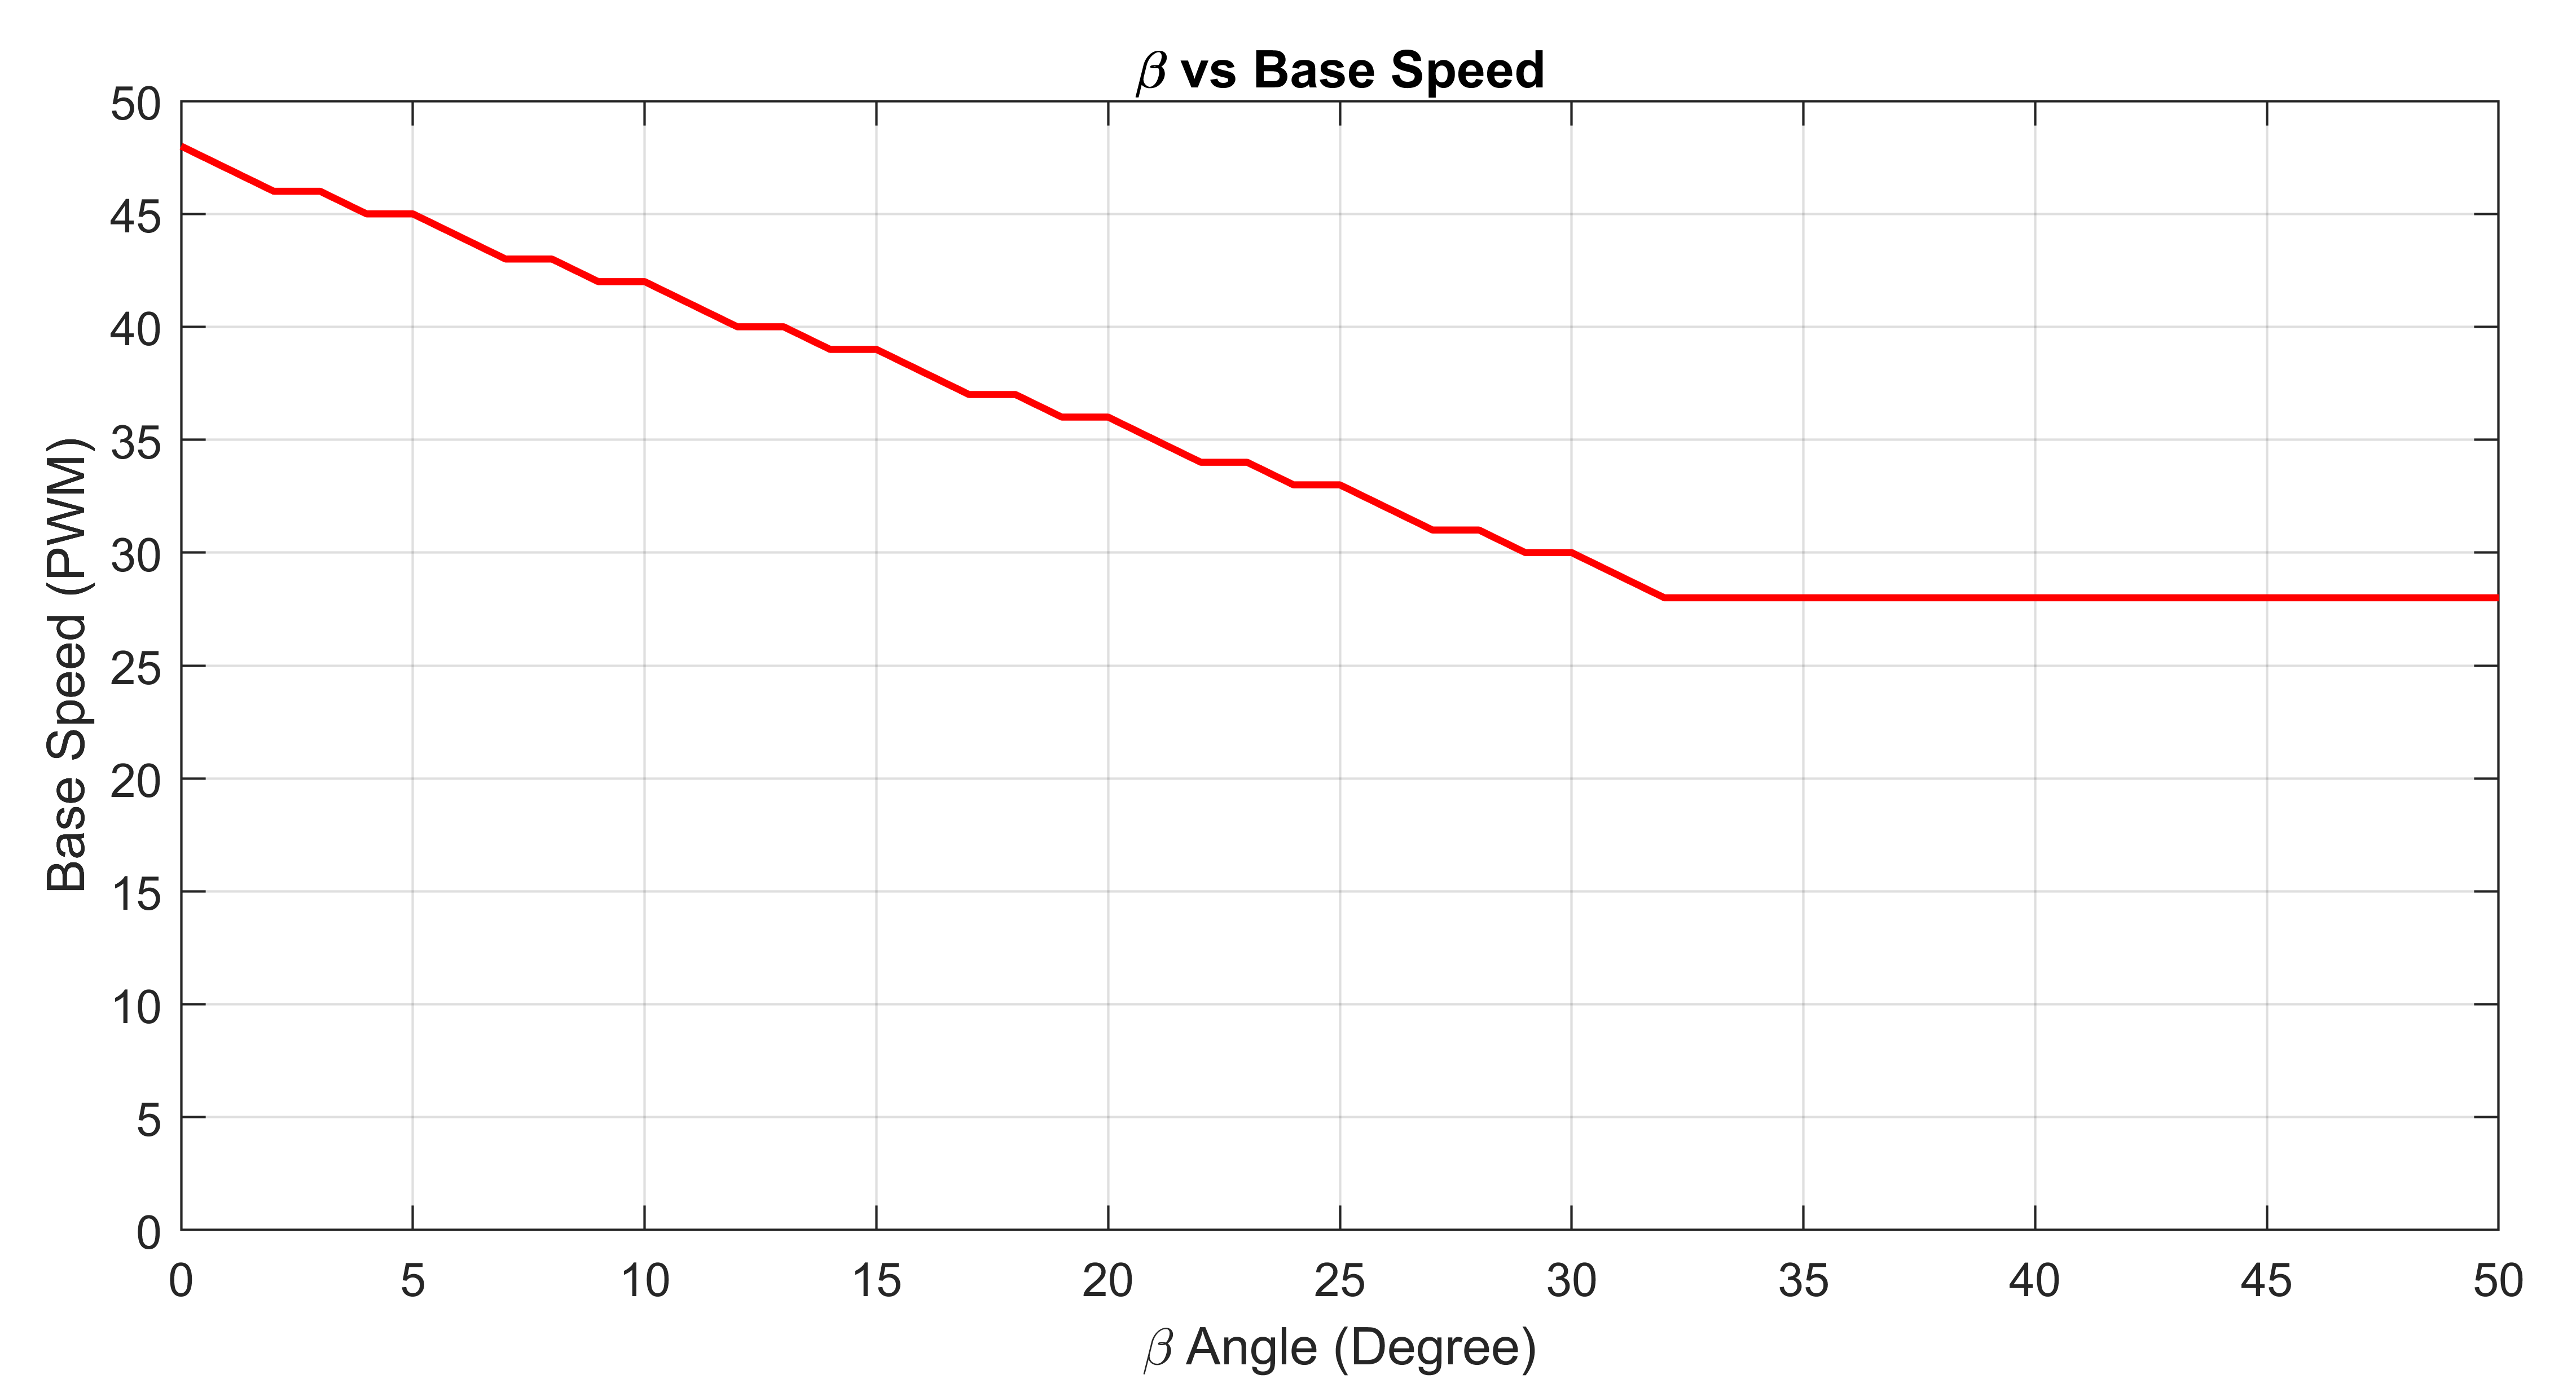
\includegraphics[width=\textwidth,center]{images/ROT_ROI/baseSpeed_crop}
		\caption{Therotical Base Speed PWM vs Theoratical $\beta$ Angle}\label{fig:baseSpeed}
	\end{figure}
	
	
	
	\item {Discussions on the Solution}
	
	The main solution idea is the same as the one proposed at \textit{Conceptual Design Review Report}. The main difference is the dependency of the base PWM value on road rotation as it was explained in \textit{Section~\ref{sect:ControllerSubsystem}}. The test results proved that the algorithm provides satisfactory performance to control longitudinal speed. 
	
\end{enumerate}

%%%%%%%%%%%%%%%%%%%%%%%%%%%
%%%%%%%%%%%%%%%%%%%%%%%%%%%


\subsection{Motion System}

	%Duty of this system is maintaining mechanical rigidity of the driving system. And the requirement for this system are as follows;

	\begin{enumerate}
		\item The system should ensure that the vehicle can drive itself with enough power.	
	\end{enumerate}	

	
	%The system has two subsystems namely,

	\begin{enumerate}
		\item \textbf{Wheels Subsystem} which is responsible for transferring power from motor shaft to road.
		\item \textbf{Motors Subsystem} which is responsible for converting electrical power to mechanical power
	\end{enumerate}

%%%%%%%%%%%%%%%%%%%%%%%%%%%

	\subsubsection{Wheels Subsystem}

		\begin{enumerate}
			\item {Requirements for the Solution}
			
			\begin{enumerate}
				\item The subsystem should ensure that the wheels can grip lane without slipping in all conditions 
			\end{enumerate}


	\item {Solution for the Subsystem}
	
	%As the previous suggestion in CDR, 2+1 combination (2 wheel with power and 1 caster ball) is preferred due to easier implementation and control. Although this placement weaker in balance and obstacle handling, importance of easier implementation and control are considered more beneficial. 
	
	%While choosing wheels, high friction property is considered. Because of this reason, super soft and slick tire are chosen with lighten aluminum rim. Besides, larger width is preferred to increase hanging on the lane.      


	\item {Discussions on the Solution}
	
	%After wheel subsystem tests, we observe the choice gives what we expect. Although tires make dirty the path, their handling capability is fascinating. Therefore, this system satisfies requirements.

	\end{enumerate}



	\subsubsection{Motors Subsystem}

		\begin{enumerate}
			\item {Requirements for the Solution}
			
			\begin{enumerate}
				\item The subsystem should ensure that the motors can supply enough torque to accelerate the vehicle 
				\item The subsystem should ensure that the motors can execute driving system outputs without deviation
			\end{enumerate} 

		\item {Solution for the Subsystem}

			%As the previous suggestion in CDR, DC motor selection did not change. The reason of this brushed gearhead DC motors are designed to this usage. Even though 3kg-cm is proposed, because the size and weight of the motors in this specs are not appropriate under 600 RPM condition, and eliminate the over engineering, this calculation turns into weight = torque at the shaft of the motor. RPM condition is set in CDR with equation (1). According to this equation 95.5 RPM is the minimum condition, but to be a strong competitor, 5 times of this value is idealized to goal speed. To handle with this value 100 RPM margin is set, to health of the motors during competition.   
	
		\item {Discussions on the Solution}

	%After motors subsystem tests, motors can move symmetrical without PWM offset, and vehicle can move fast enough with the motors. Also, they perform well in differential drive operation. Therefore, this system satisfies requirements. 

	\end{enumerate}	





\subsection{Structure System}

	%This system is responsible for mechanical structure of the vehicle. Placement and orientations of both electrical and mechanical components are considered in this system. And the requirements for this system are as follows;


	\begin{enumerate}
		\item The system should	ensure that structure is robust for external effects 
		\item The system should	ensure that structure is balanced
		\item The system should ensure that vehicle has a good appearance
	\end{enumerate}	


	The system has two subsystems namely,
	
	\begin{enumerate}
		\item \textbf{Chassis Subsystem} which is responsible for the connections of mechanical components in the vehicle.
		\item \textbf{Printed Circuit Board Subsystem} which is responsible for the placement of electrical components.
	\end{enumerate}

%%%%%%%%%%%%%%%%%%%%%%%%%%%
%%%%%%%%%%%%%%%%%%%%%%%%%%%

\subsubsection{Chassis Subsystem}

	\begin{enumerate}
		\item {Requirements for the Solution}
		
		\begin{enumerate}
			\item The subsystem should ensure that the chassis is rigid 
			\item The subsystem should ensure that the chassis have enough space for components
			\item The subsystem should ensure that the chassis can provide low center of mass 
			\item Camera holder should be integrated to the front of the vehicle
			\item Camera holder should be as rigid as possible to reduce the vibration on the camera
			\item Camera holder should be light weight so that does not effect the center of mass considerably
			\item Camera holder should be adjustable in terms both elevation and camera angle
		\end{enumerate}


	\item {Solution for the Subsystem}

		%Main purposes of this subsystem are protection of the critical elements of the robot and holding components together. The most important part of this section is weight distribution.\\

		%Current chassis structure relies on two newly-designed plexiglass layers. Raspberry Pi and Arduino is placed on the upper layer while motor driver and the battery are on lower one. To keep the center of mass of the vehicle close to the ground, battery is placed as low as possible. The connection of the motor driver and Arduino consists of eight cables two of which are the power lines. The cables are placed in a way that they cause no entanglement with any other parts. The connection between RPi and Arduino is currently accomplished by USB cable. \\

		%Since there is not much component on the vehicle, the space on the layers are enough to locate the components. However, placing the camera of RPi has been a great problem. The view angle of the camera turned out to be considerable small than expected. Other several cellphone cameras were tried but they are could not satisfy the requirement that both side of the lane should be visible either. The only solution was to elevate the camera. That is why a camera holder structure is designed and added to the system.\\	

		%To satisfy the requirements the holder is built using 4mm plexiglass. The choice satisfies the rigidity and light weight possible. A thinner one would result in less rigidity and increased vibration on the system. The designed structure has the elevation range from 35 cm to 45 cm and a camera angle ranging from $0^o$ to $45^o$. Having manufactured, the camera holder is integrated to the vehicle (\textit{see Figure \ref{fig:chassis}}). After integration, the view of the camera can completely cover the both edges of the path.\\

		%In addition, new motor holder part is designed to have better connection of the wheels to the vehicle. 3D isometric view of the piece can be seen in \textit{Figure }.

	\begin{figure}[h]
		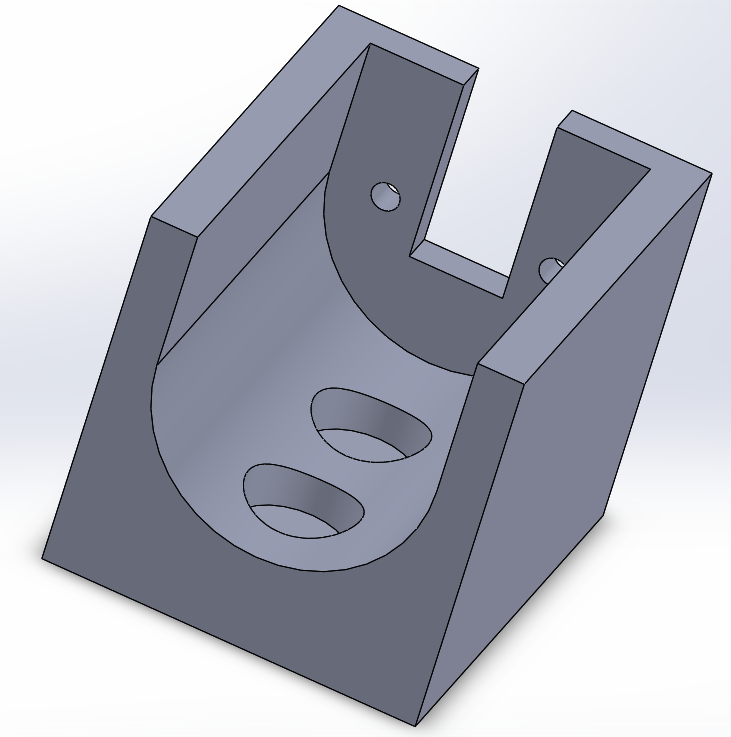
\includegraphics[width=.2\textheight,center]{images/motor-holder.png}
	\caption{Motor holder 3D view}
	\end{figure}


	Current version of chassis can be seen in \textit{Figure~\ref{fig:chassis}}.


	\begin{figure}[h]
		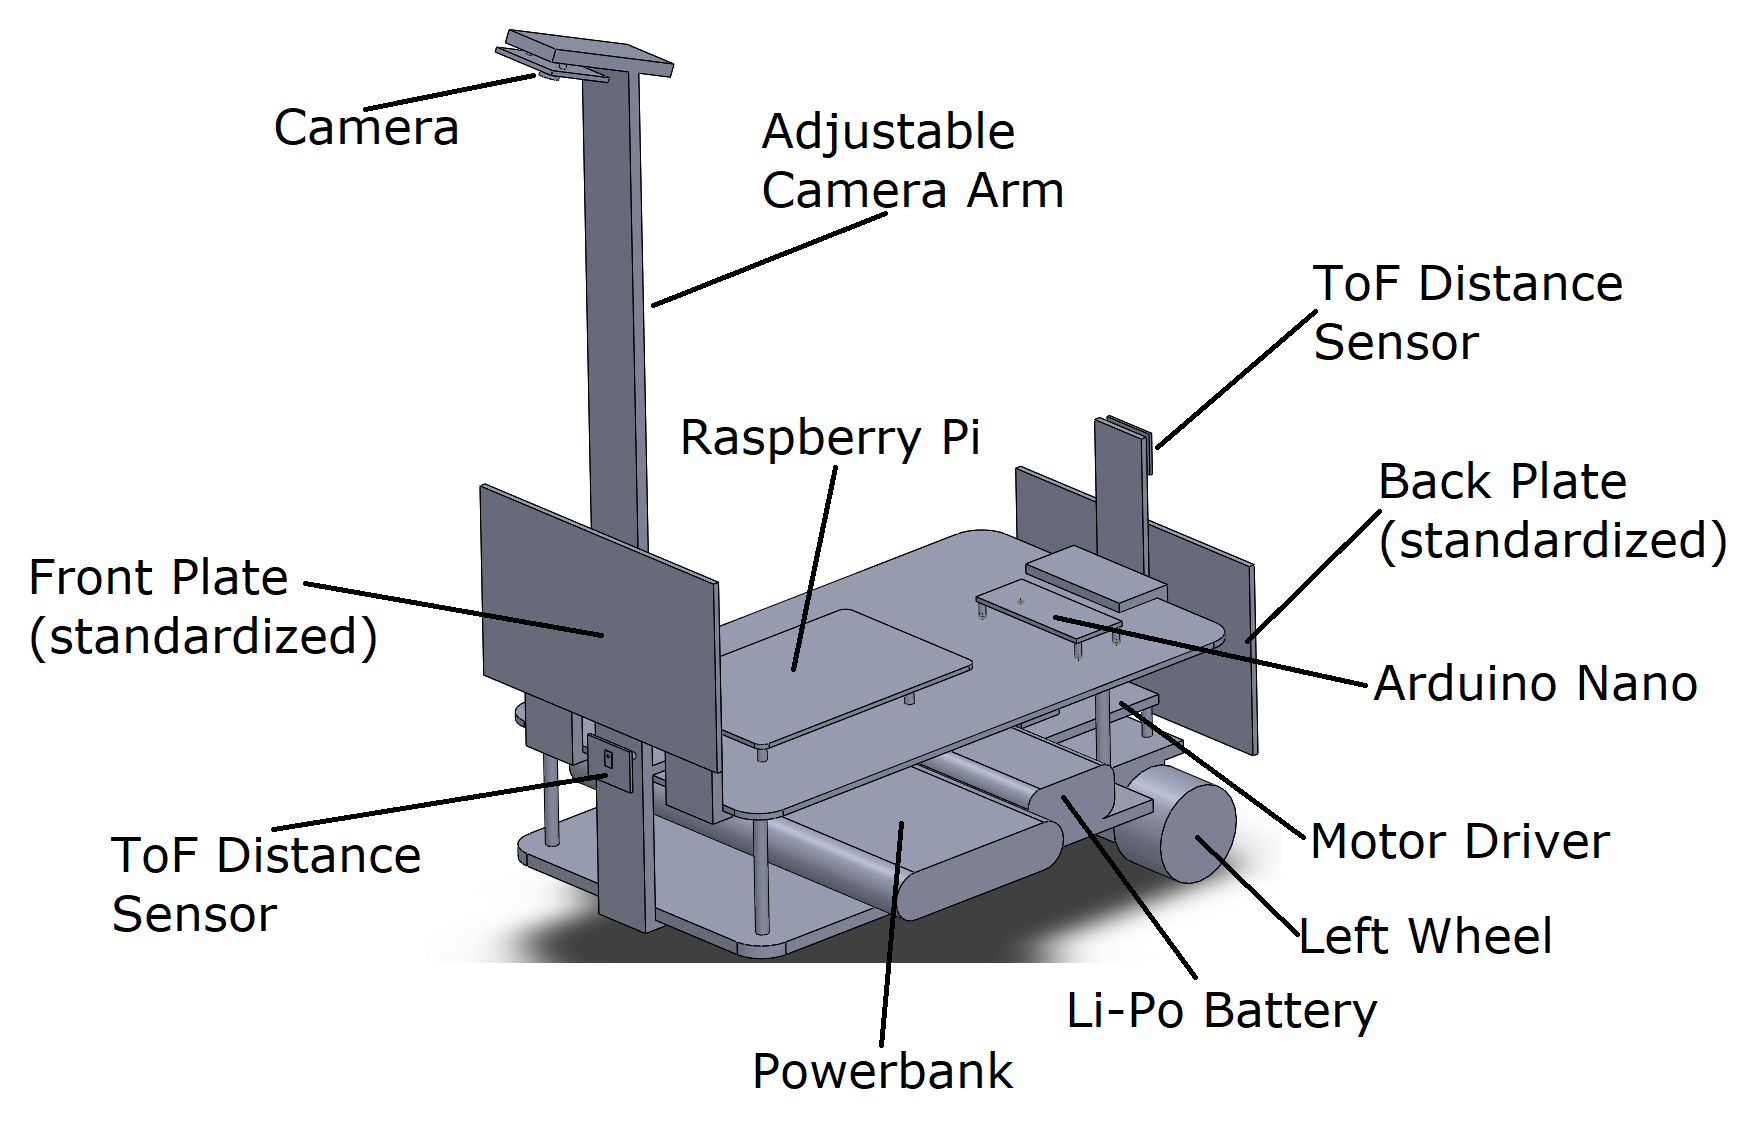
\includegraphics[width=0.8\textwidth,center]{images/chassis1}
		\caption{Isometric view of the 3D Drawing of the Vehicle \label{fig:chassis} }
	\end{figure}

	\item {Discussions on the Solution}

		%The only change done on this subsystem is to design a new plexiglass layers instead of using pre-designed ones. By that way, much more flexibility is obtained in terms of placement of the components. On the other hand designed motor holder pieces provides rigid connection between chassis and the wheels.  

	\end{enumerate}


%%%%%%%%%%%%%%%%%%%%%%%%%%%
%%%%%%%%%%%%%%%%%%%%%%%%%%%

\subsubsection{Printed Circuit Board Subsystem}

	\begin{enumerate}
		\item {Requirements for the Solution}
		
		\begin{enumerate}
			\item The subsystem should ensure that all the electronic components are placed on PCB
			\item The subsystem should ensure that all the connections are firmly secured and robust to vibrations.
		\end{enumerate} 

	\item {Solution for the Subsystem}

		%The main role of this part is decreasing connection mess and increase vibration strength of the robot against disturbances. Also, this section increases rigidity of the whole system. The requirements of this subsystem are listed below:	

		%This subsystem aims to make all the circuit connections rigid and compact. Currently, there is wire connections between Arduino-Motor driver and Arduino-RPi. However, addition of vehicle detection sensors and other lane detection alternatives will increase the amount of components, hence, wires. In addition, to use the space occupied by the Arduino UNO board, Arduino Mini can be used. This also allows to build the circuit board as shield for Arduino Mini. After that any other sensors and connections can be made through PCB. In other words, PCB acts as a breakout board for each item integrated to the system in a more rigid and compact way.


	\end{enumerate}	


%%%%%%%%%%%%%%%%%%%%%%%%%%%
%%%%%%%%%%%%%%%%%%%%%%%%%%%


\subsection{Compatibility of the Subsystems}

	The block diagram showing the interaction of the subsytem block with each other can be seen from the \textit{Figure~\ref{fig:subsys-block}}. As can be seen from the figure also that, there are two main path within the project. One of them starts by processing the camera vision by the \textit{Lane Detection Subsystem} and ends with the transfer of torque from \textit{Motors Subsystem} to \textit{Wheels Subsystem} which results with a movement of the vehicle. In this path the data before the \textit{PID Controller} and \textit{Speed} subsystems are processed within the Raspberry Pi without any problem, at this point the output data are transferred to Arduino by \textit{Internal Communication Subsystem} without any problem. The rest of this path is processed by the Arduino without any problem as well.

	The second path starts with the detection of the opponent by the \textit{Vehicle Detection Subsystem}. The path continues within the Raspberry Pi until the \textit{vehicle stop signal} is transferred to \textit{Motors Subsystem} by \textit{Internal Communication Subsystem} without any problem.

	\begin{figure}[h]
		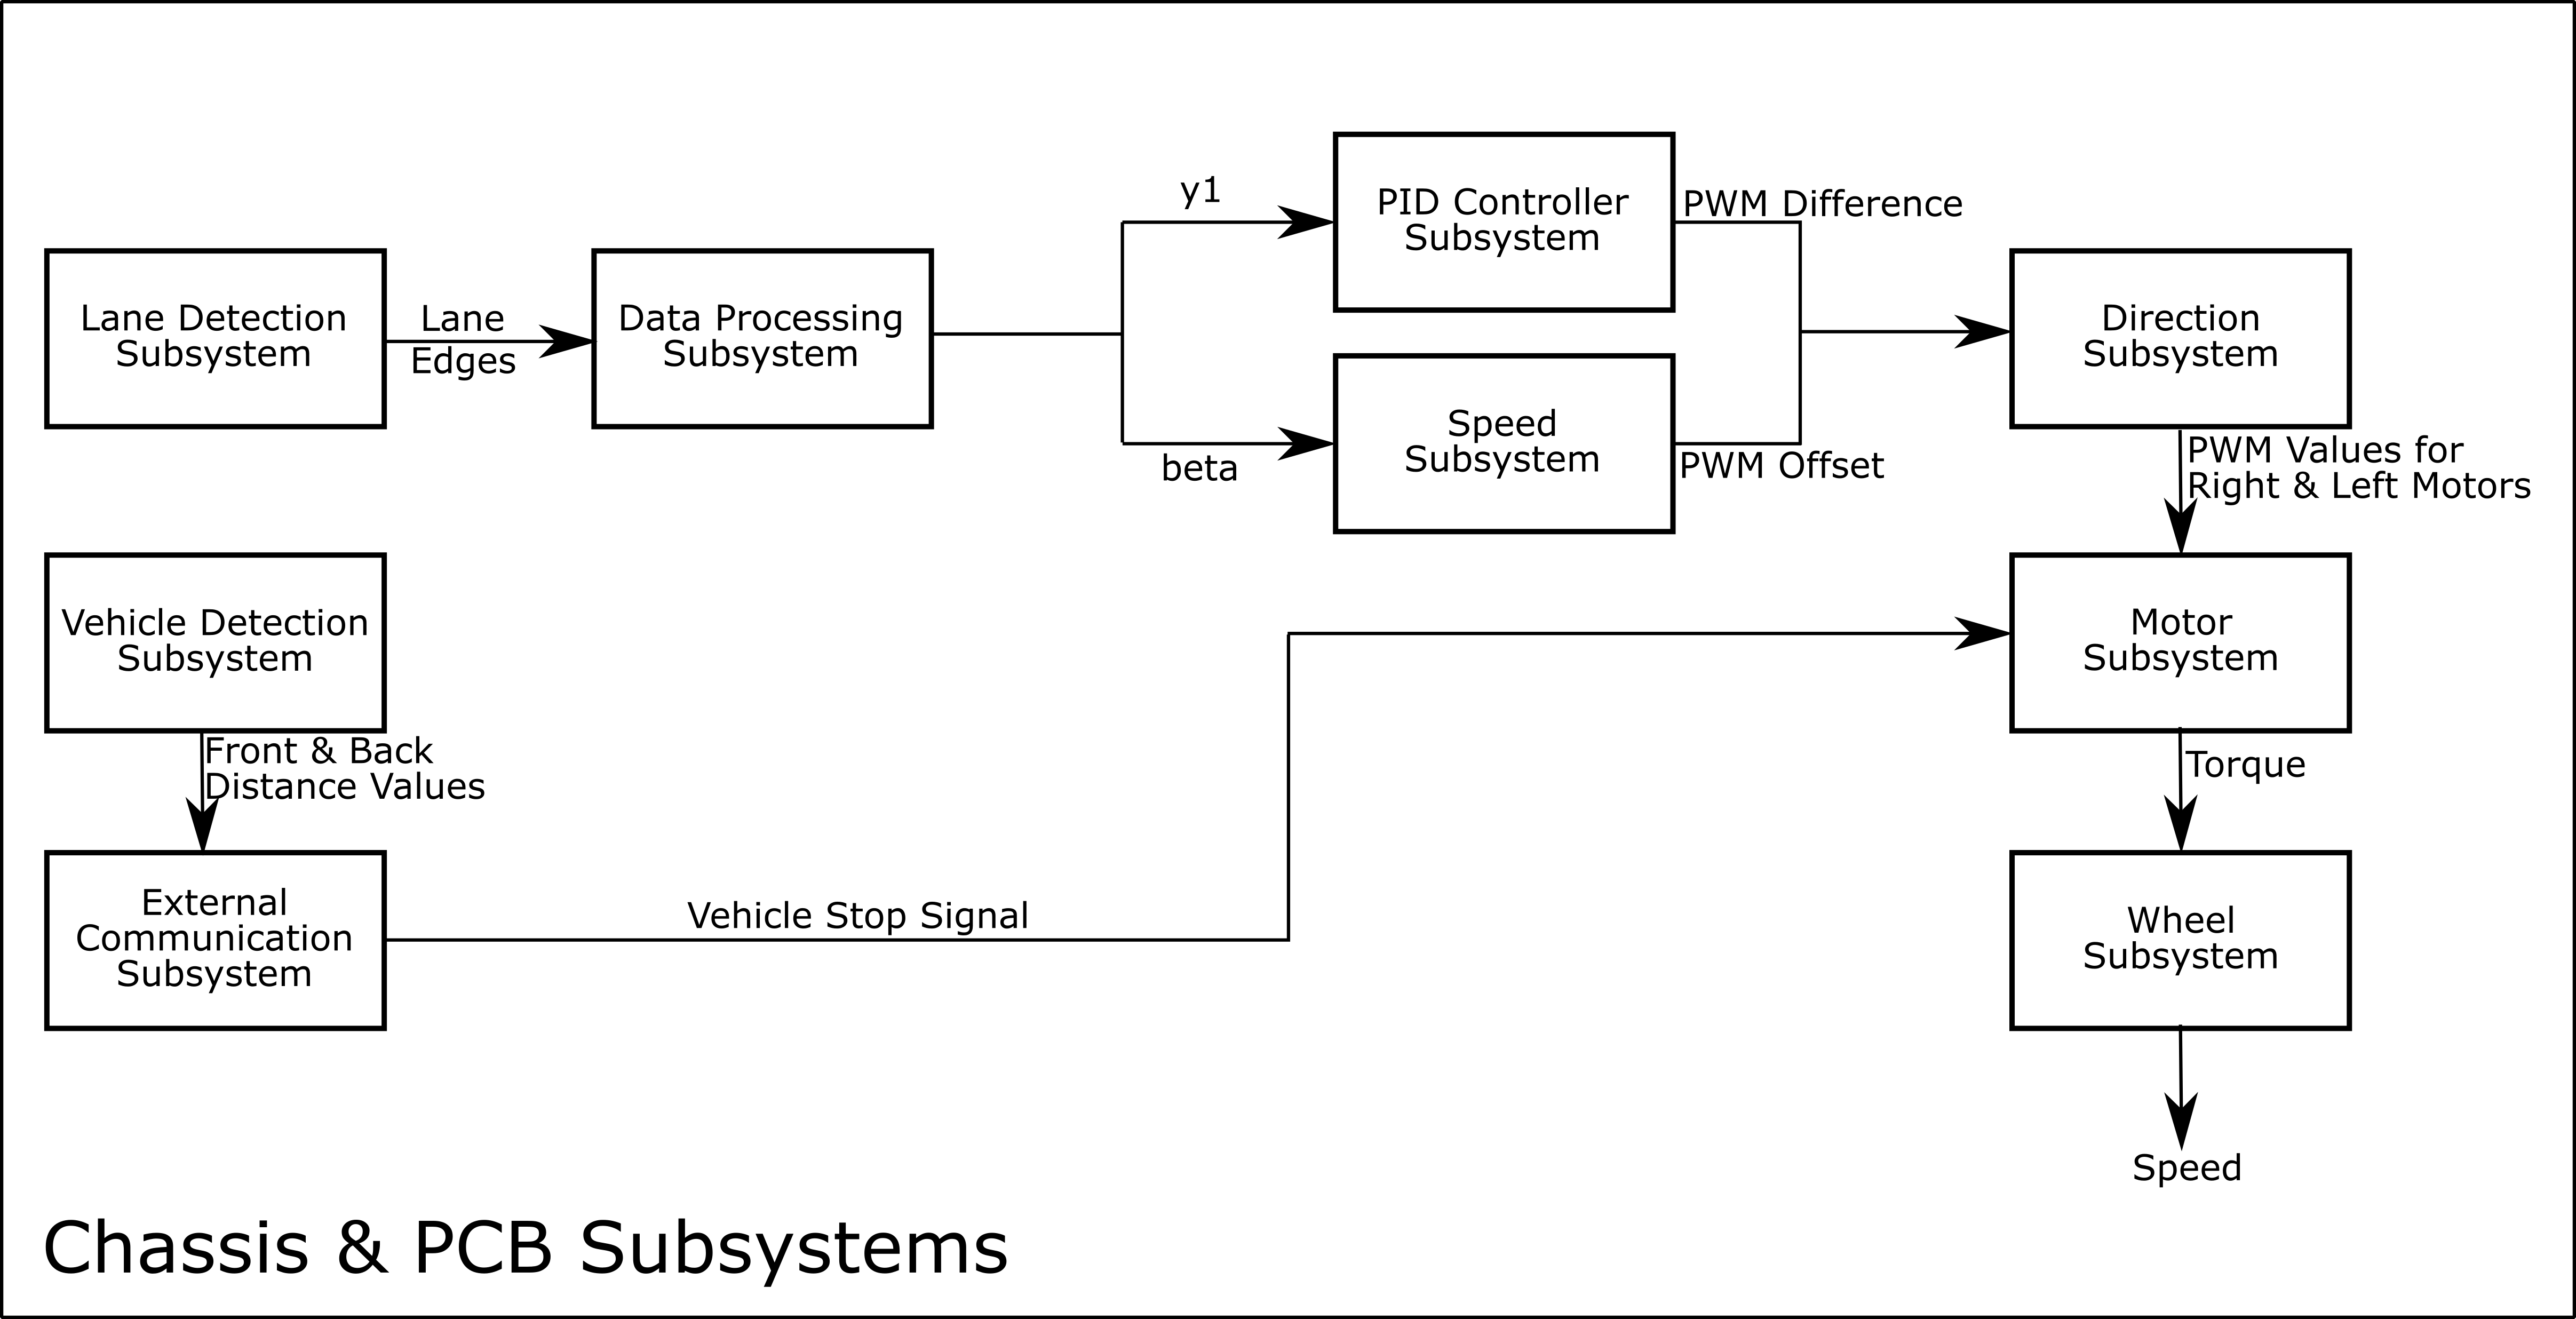
\includegraphics[width=\textwidth,center]{images/subsys_block}
		\caption{Block Diagram of the Project and the Interaction of the Subsystems}\label{fig:subsys-block}
	\end{figure}

%%%%%%%%%%%%%%%%%%%%%%%%%%%
%%%%%%%%%%%%%%%%%%%%%%%%%%%






\section{Detailed Tests for the Subsystems}\label{test_sec}
	This section presents followed test procedures and the outcome of the tests.
%%%%%%%%%%%%%%%%%%%%%%%%%%%

\subsection {Lane Detection Subsystem Tests and Results}	


\begin{enumerate}

\item{Light Condition Test}

\begin{enumerate}

\item Mirror the Raspberry Pi screen into Laptop via VNC  

\item Execute the lane detection algorithm in Raspberry Pi 

\item Change the location of the camera and Pi to conduct test 

\item Observe the results in different locations   

\item If the visible lane sides can be detected without any additional object, the result of the test can be considered as success. 

\end{enumerate}

\item{Visual Disturbance Test}

\begin{enumerate}

\item Mirror the Raspberry Pi screen into Laptop via VNC   

\item Execute the lane detection algorithm in Raspberry Pi  

\item Put different objects into lane  

\item Observe the results with different disturbances 

\item If the objects outside of lane is not detected and the objects inside the road only detected only at its border with road, the result of the test can be considered as success.  

\end{enumerate}

\end{enumerate}


\subsubsection*{Results of Lane Detection Subsystem Tests}

	The lane detection tests are conducted to asses reliability of the detection pipeline. A sample test result is shown in \textit{Figure~\ref{fig:laneD_test}}. The tests reveal that the subsystem satisfies its requirements by detecting lane lines. Note that, not all lines are detected, only the lines that are in the ROI are detected. One thing to note for the robustness of this subsystem is subsystem works as expected long as HSV filter is tuned for the medium.


	\begin{figure}[h]
		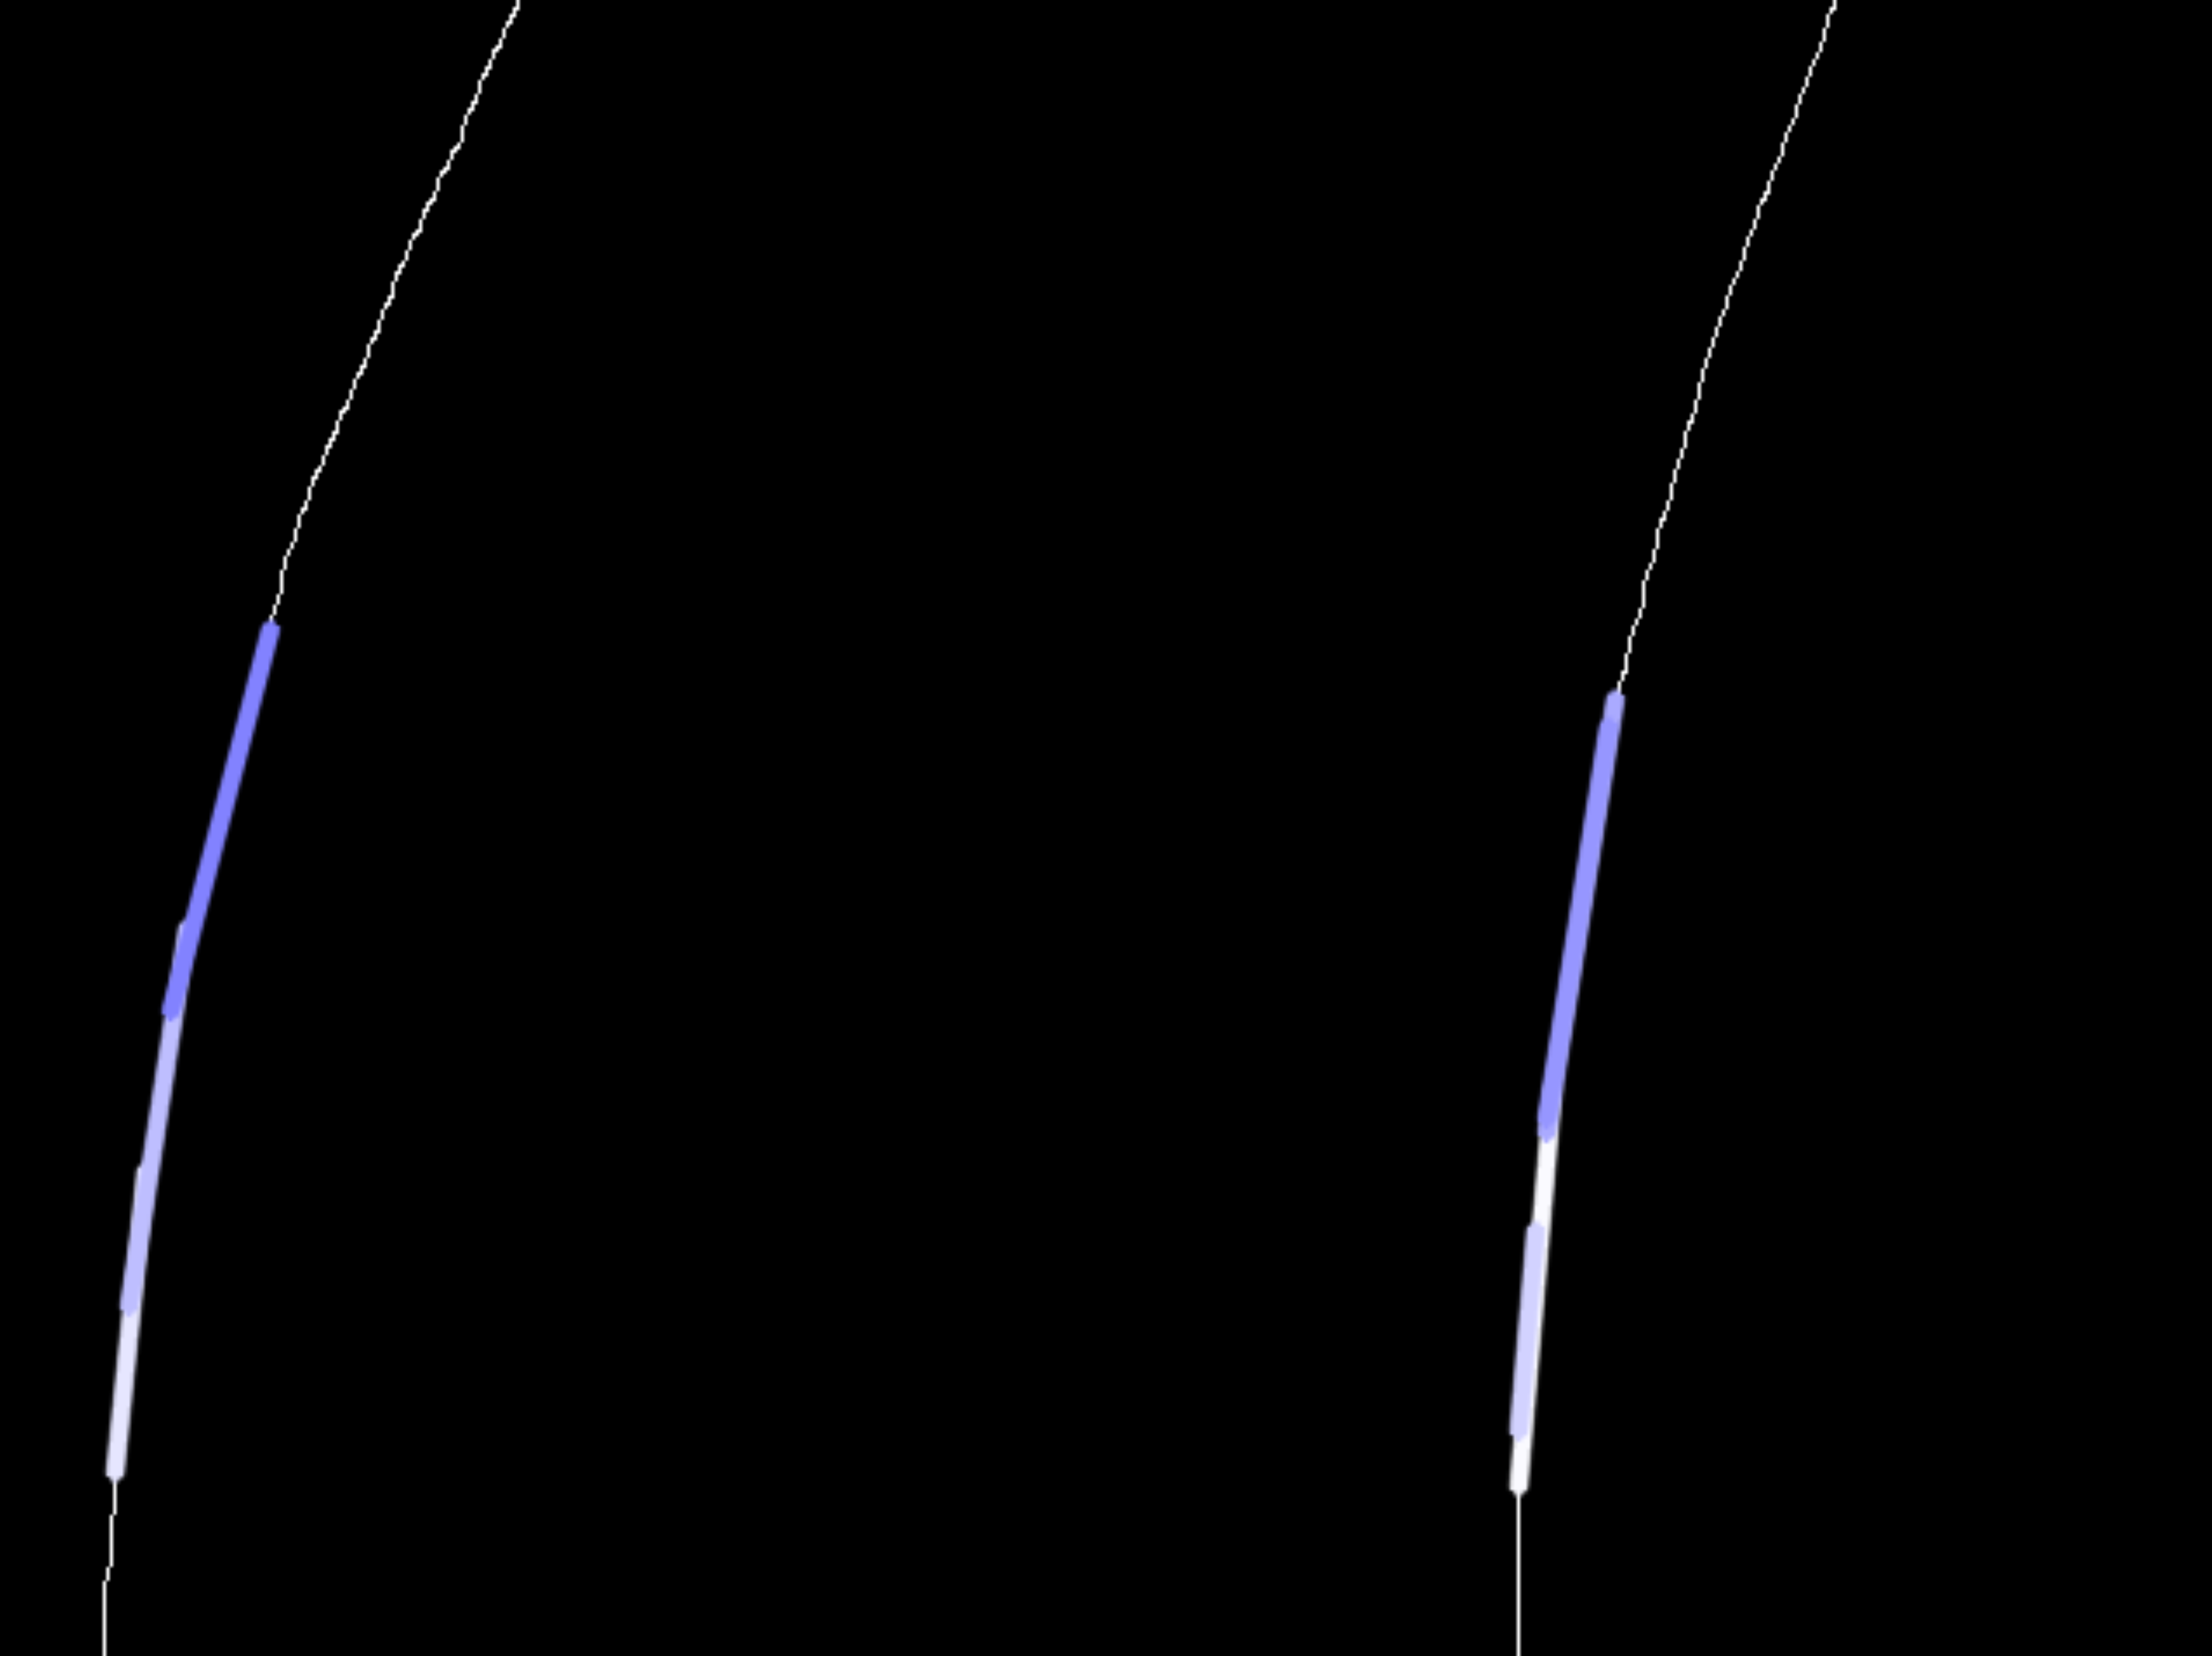
\includegraphics[width=0.75\textwidth,center]{images/laneD_test}
		\caption{Lane Detection Test Result \label{fig:laneD_test} }
	\end{figure}





%%%%%%%%%%%%%%%%%%%%%%%%%%%

\subsection {Vehicle Detection Subsystem Tests and Results}\label{sect:vhd}


\begin{enumerate}
	\item Vehicle Detection Test in Closed Environment with One Sensor:
	
	\begin{enumerate}
		\item Make the connection of the desired sensor and Pi properly  
		\item Hold the sensor at an angle of 90 degree with respect to ground  
		\item Place the test object 5 cm in front of the desired  
		
		\item Observe the output of the subsystem  
		
		\item Repeat the step 3 \& 4 with different distances  
		
		\item If the output of the subsystem is very closed to the actual measurement (i.e., with an error rate approximately 1 percent) the test result can be considered as success.
		
	\end{enumerate}					
	
	
	\item Vehicle Detection Test in Closed Environment with Two Sensors:		
	
	\begin{enumerate}
		
		\item Repeat the test steps of the \textit{Front Vehicle Detection Test in Closed Environment with One Sensor} when both sensors are connected to the rear of the vehicle.   
		
	\end{enumerate}
	
	
	\item {Angled Approach Test:}
	
	\begin{enumerate}
		
		\item Make the connection of the desired sensor and Pi properly  
		
		\item Hold the sensor at an angle of 90 degree with respect to ground  
		
		\item Place the test object 5 cm in front of the sensor with 30 degree angle with respect to the sensor  
		
		\item Observe the output of the subsystem  
		
		\item Repeat the step 3 \& 4 with different distance and angle values  
		
		\item If the output of the subsystem is very closed to the actual measurement (i.e., with an error rate approximately 1 percent) the test result can be considered as success. 
		
	\end{enumerate}
	
	
	\item Vehicle Detection in Different Sunlight Conditions Test:
	
	\begin{enumerate}
		
		\item Repeat the test steps of the \textit{Front Vehicle Detection Test in Closed Environment with Two Sensors}  in CCC (Cultural and Convention) ground under direct sunlight  
		
		\item Repeat step 1 in CCC (Cultural and Convention) under artificial light, in other words, under no direct sunlight conditions  
		
		\item Repeat steps 1 \& 2 for different locations of E Building including Graduation Laboratory  
		
		\item If the output of the subsystem is very closed to the actual measurement (i.e., with an error rate approximately 1 percent) the test result can be considered as success. 
		
	\end{enumerate}
	
	
	
\end{enumerate}
	
	\subsubsection*{Results of Vehicle Detection Subsystem Tests}
	
	
	All the test procedures mentioned at the \textbf{Section~\ref{sect:vhd}} is applied to the VL6180X Time-of-Flight distance sensor. At first, test results were satisfying for the back sensor, but not for the front one. Tests were repeated with switching front and rear sensors. Again, the sensor in the front of the vehicle measured erroneously. Then it is realized that the position of the front sensor is problematic. In the first design of the chasis, the front sensor was placed behind a hole under the the stick supporting camera. It is realized that this configuration was blocking the sensor. Then, in the second chasis design, front sensor is brought in front of the stick. After repeating tests results, it is confirmed that the problem with the front sensor is eliminated. 
	
	Time-of-flight sensors show very accurate result inside the closed environments like laboratory under artificial lights. The results under direct sunlight especially in CCC is also good as expected. In addition to the success in different light conditions test, the sensor shows very accurate result especially in \textit{Angled Approach Test}. According to test, the sensor gives correct results up to 30 degrees. Considering the fact that the path itself is elliptical and there would always be an angle between vehicle even though it may be very small for some cases, it is confirmed that time of flight sensors are quite good choice for this subsystem. 
	

%%%%%%%%%%%%%%%%%%%%%%%%%%%



\subsection {Data Processing Subsystem Tests and Results}	

\begin{enumerate}

\item Data Assessment Test

\begin{enumerate}

\item Link the output of Lane Detection subsystem to Data Processing subsystem.  

\item Asses if the output coincide with physical reality of the path  

\end{enumerate}

\item Output Stability Test

\begin{enumerate}
	
	\item Place the vehicle on a fixed point on the path
	
	\item Observe the variation of the control outputs
	
\end{enumerate}

\end{enumerate}
\subsubsection*{Results of Data Processing Subsystem Tests}\label{sec:DataProcessingSubsystemTests}

	The tests asses the ability and performance of the subsystem. Numerous tests are made. The first set of tests cover the robustness of the subsystem by placing an obstacle of the subsystem. The test scenario and its results are presented in \textit{Figure~\ref{fig:dataP_down},\ref{fig:dataP_up} and \ref{fig:dataP_par}}. It can be seen that the algorithm ignores the obstacles in 7 cases out of 9 tests. In two cases, the algorithm fails to ignore the obstacles and determines the steering angle as if obstacle constitutes the lane line. Besides the results, on the presence of obstacles, in some particular obstacle placements, the output of the subsystem is observed to be unstable. Since the implementation is frozen after Conceptual Design Report, there has not been any significant change in the test performances since then.

	The second set of tests cover the robustness of the subsystem as well, but under changing lighting conditions and on different surface materials. The results of this test is presented in \textit{Figure~\ref{fig:dataP_inside} and \ref{fig:dataP_outside}}. The presented results are promising, the steering angles are true. A problem is that these results are a bit unstable when the luminosity difference between the shadows and flighty parts increase. The shadows are sometimes detected as lines and cause untrue lane line evaluations.	
	
	The third and the last test is  made to see if the outputs are consistent when the vehicle is fixed on a point on the path. This test reveals the robustness of Data Processing Subsystem as it gives a measure on the stability of control outputs. PID Controller can work as expected, only if the provided inputs are predictable and repeatable. The test case and the results are given in \textit{Figure~\ref{fig:stabilityTestI-dist}, ~\ref{fig:stabilityTestS-dist} and ~\ref{fig:stabilityTestU-dist}}. Statistical measures graphical data is also visible in \textit{Table~\ref{tab:statisticalStability}}. The stability test is satisfactory, as the variance of the three measurements are quite low.
	
		\begin{table}[H]
		\centering
		\caption{Statistical Stability Results}
		\begin{tabular}{c|c|c|c|c}
			$$ Test $$ & $$mean($\beta$)$$ & $$variance($\beta$)$$ & $$mean(y1)$$ & $$variance(y1)$$ \\ \hline
			Straight Area & -3.3 & 0.7 & 3.7 & 0.2   \\ \hline
			Bend Area & -12.3 & 0.2 & -15.6 & 0.1   \\ \hline
			Curved Area & -21.8 & 1.8 & -44.5 & 0.5 
		\end{tabular} 
		\label{tab:statisticalStability}
	\end{table}

\begin{figure}[H]

\setlength{\unitlength}{\textwidth} 

\centering

\begin{subfigure}{.31\textwidth}

\centering

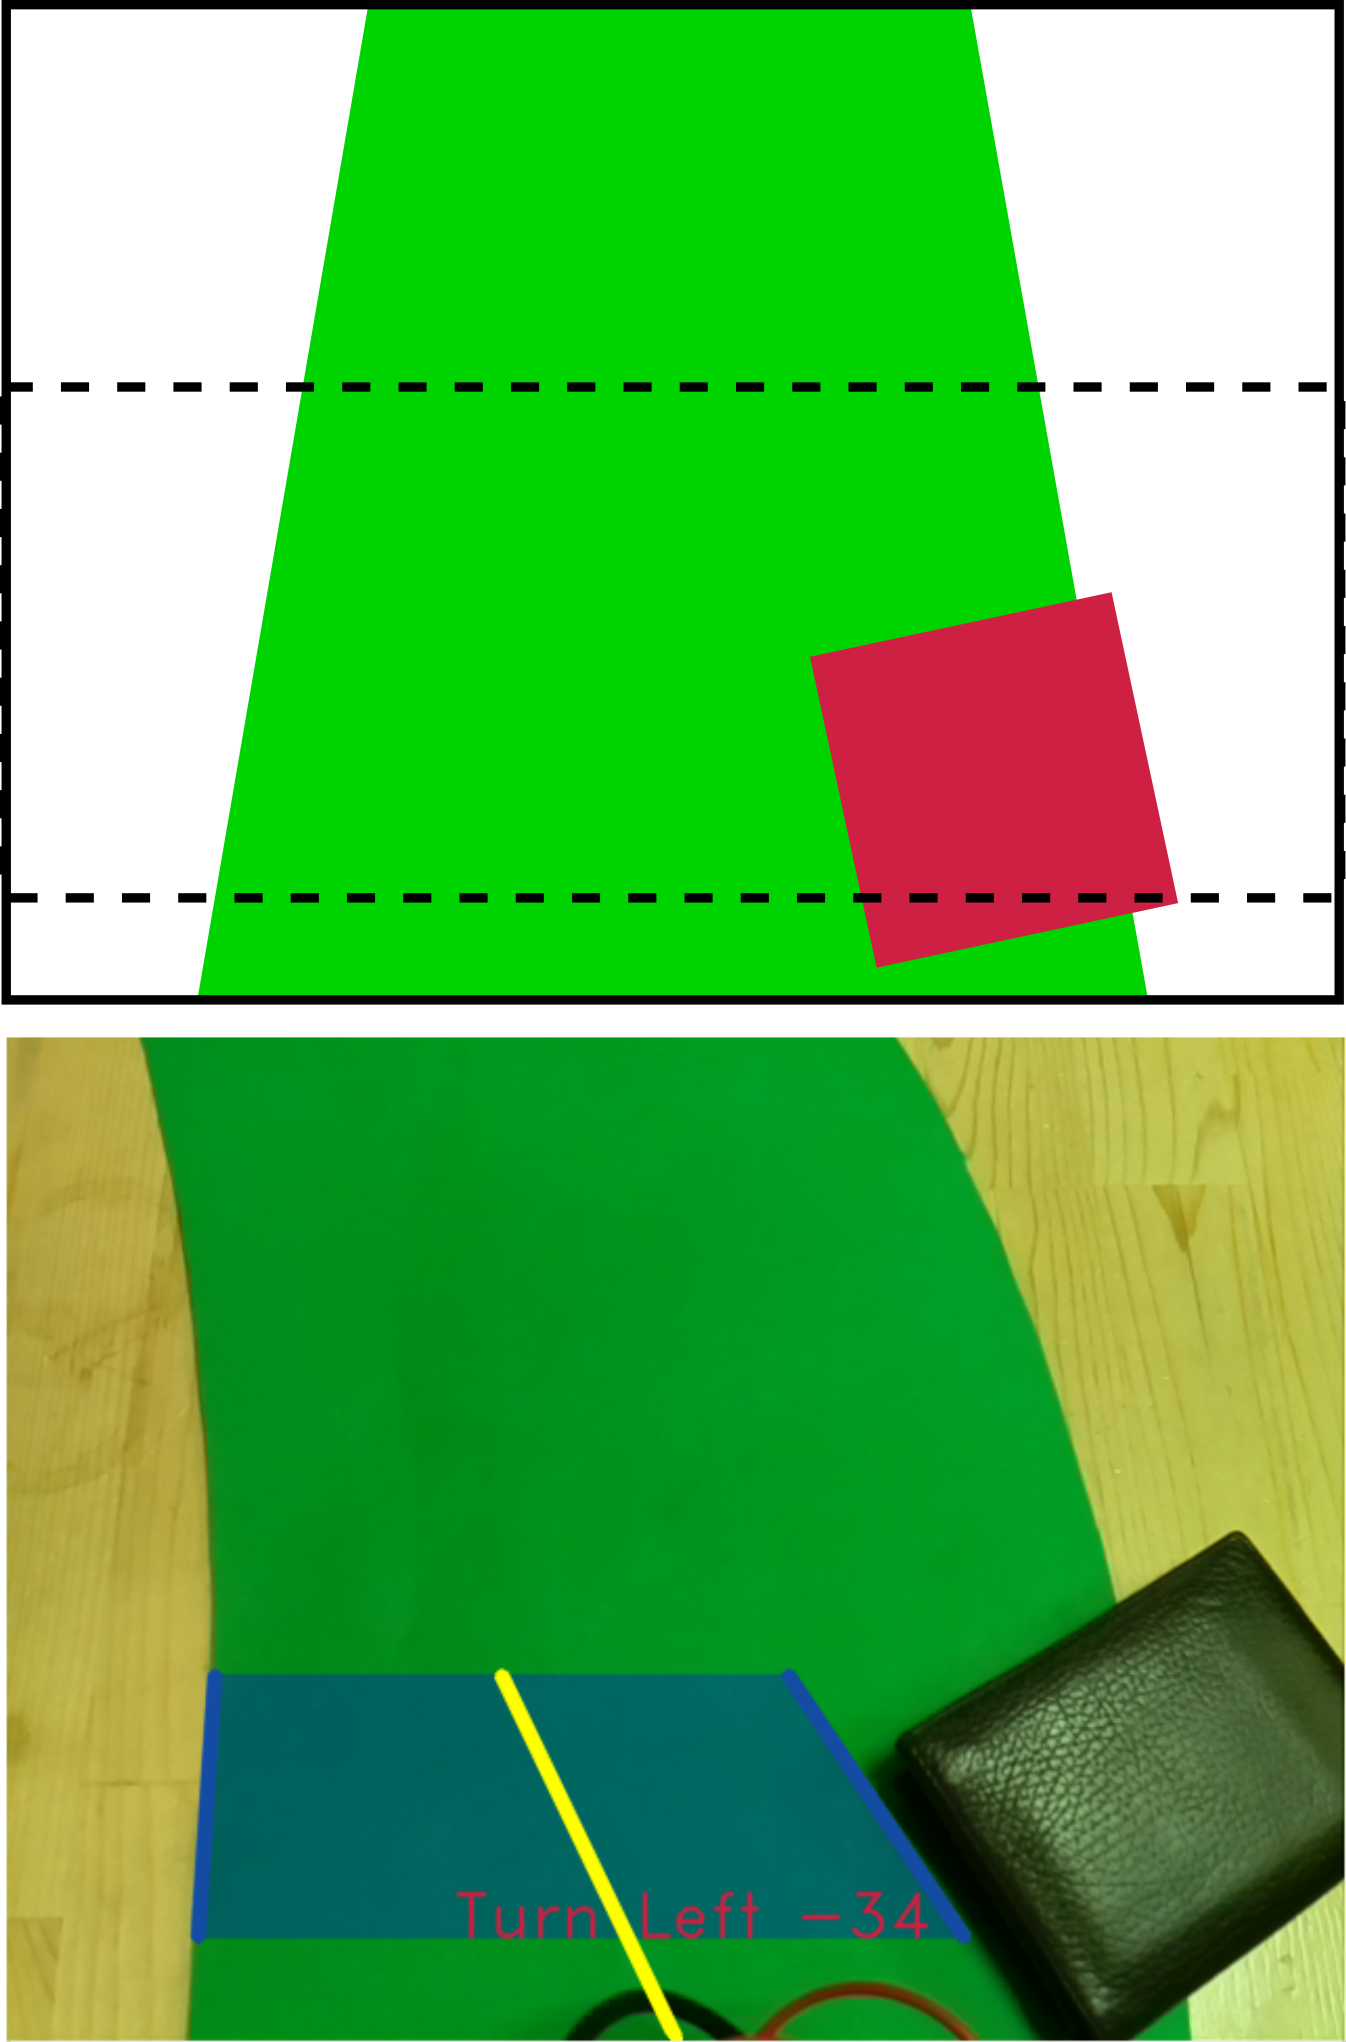
\includegraphics[width=0.30\unitlength]{images/path_images/down_1}

\caption{\label{fig:dataP_down_1} Obstacle is at the Beginning of the Path}

\end{subfigure}%
\begin{subfigure}{.31\textwidth}

\centering

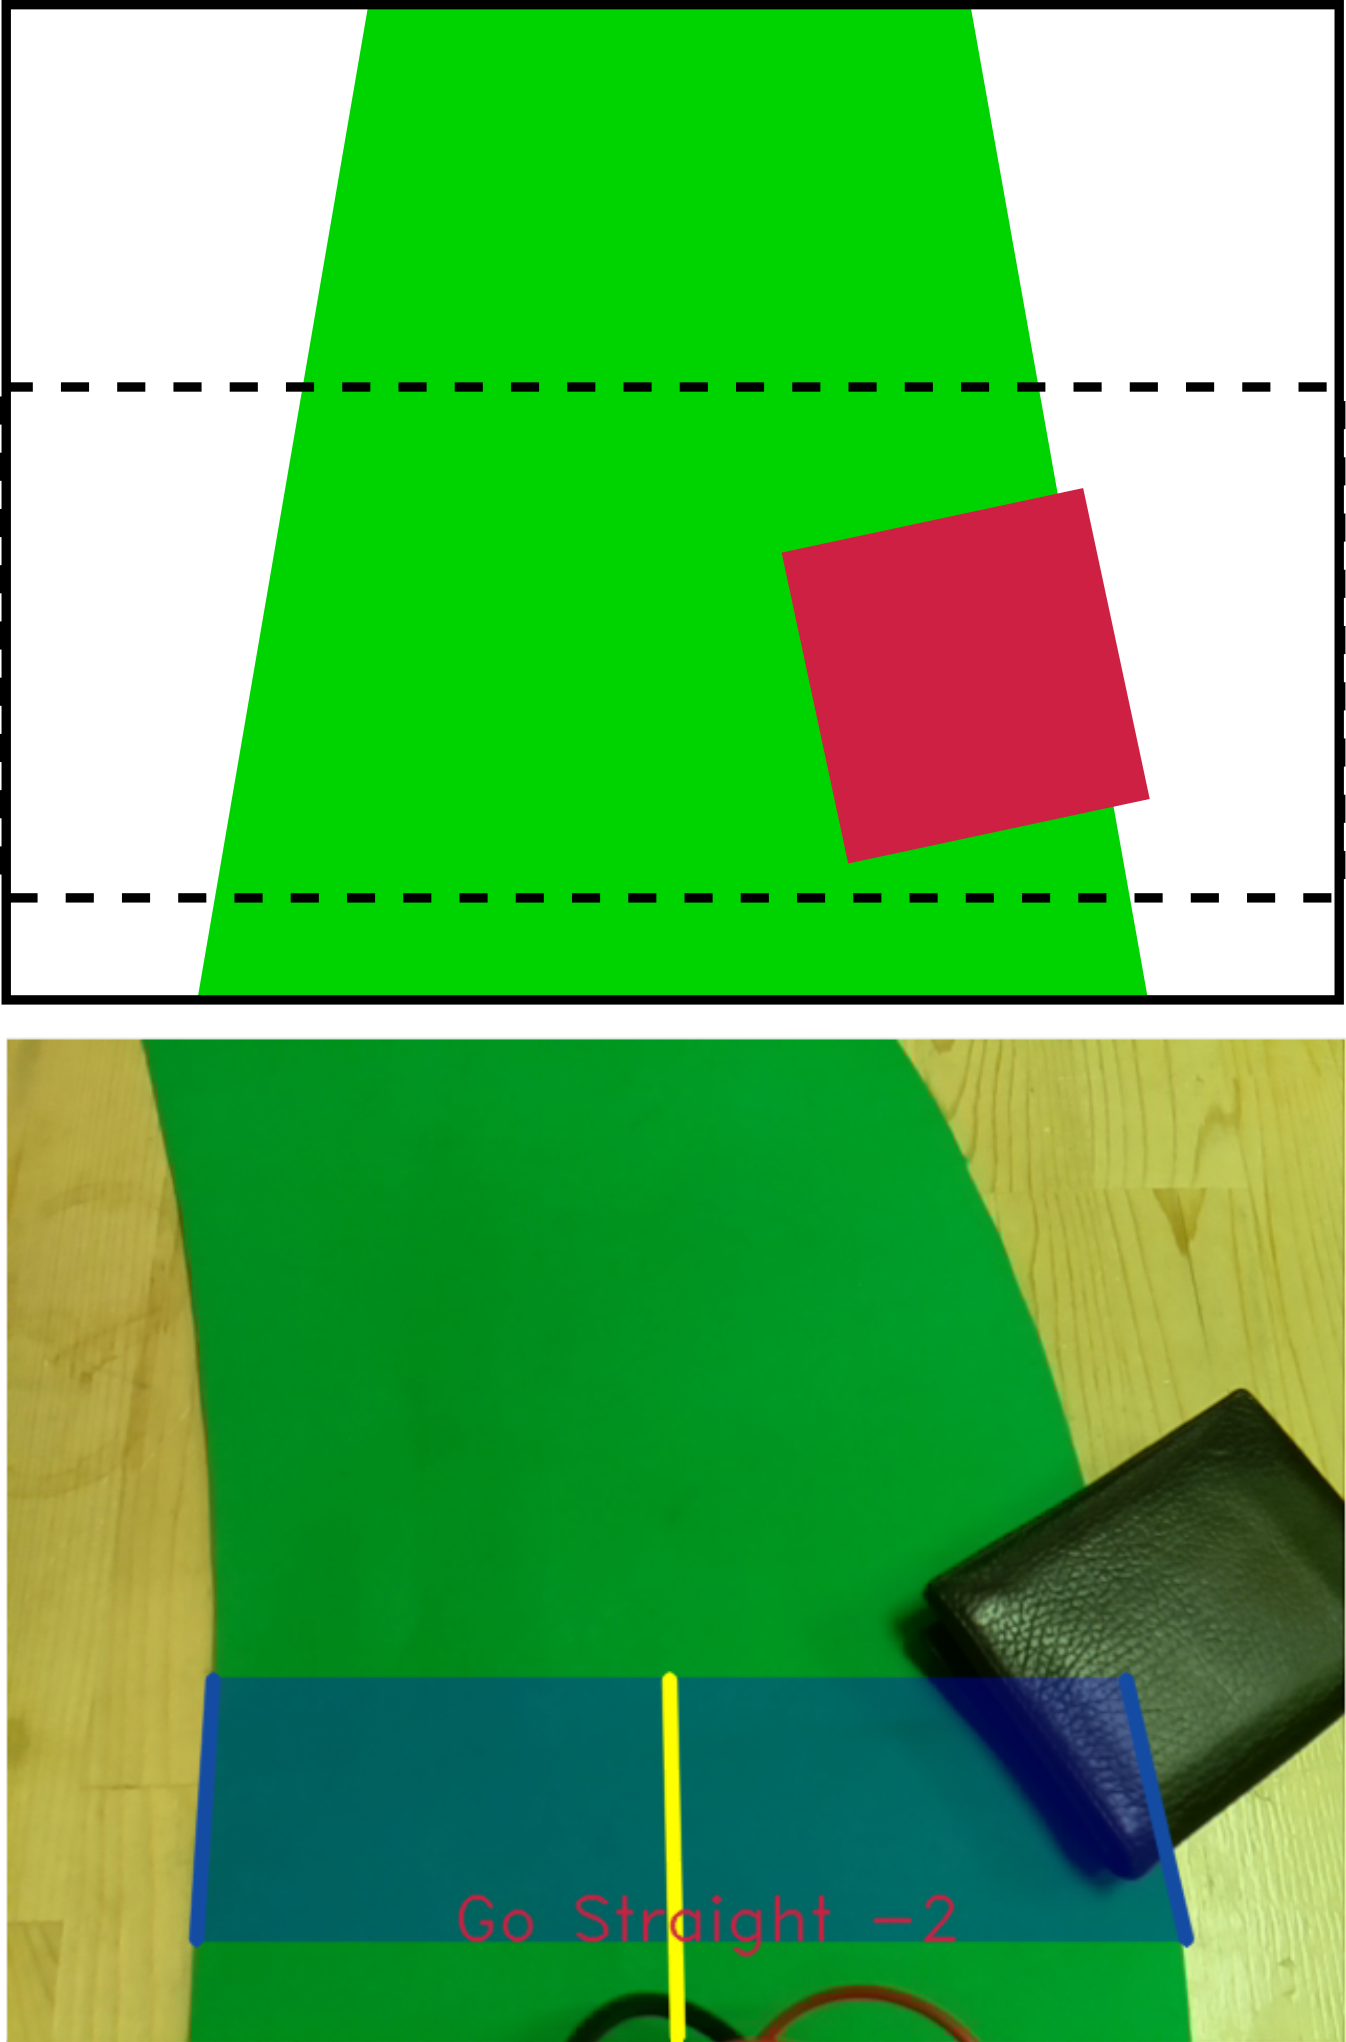
\includegraphics[width=0.30\unitlength]{images/path_images/down_2}

\caption{\label{fig:dataP_down_2} Obstacle is at the Middle of the Path}

\end{subfigure}
\begin{subfigure}{.31\textwidth}

\centering

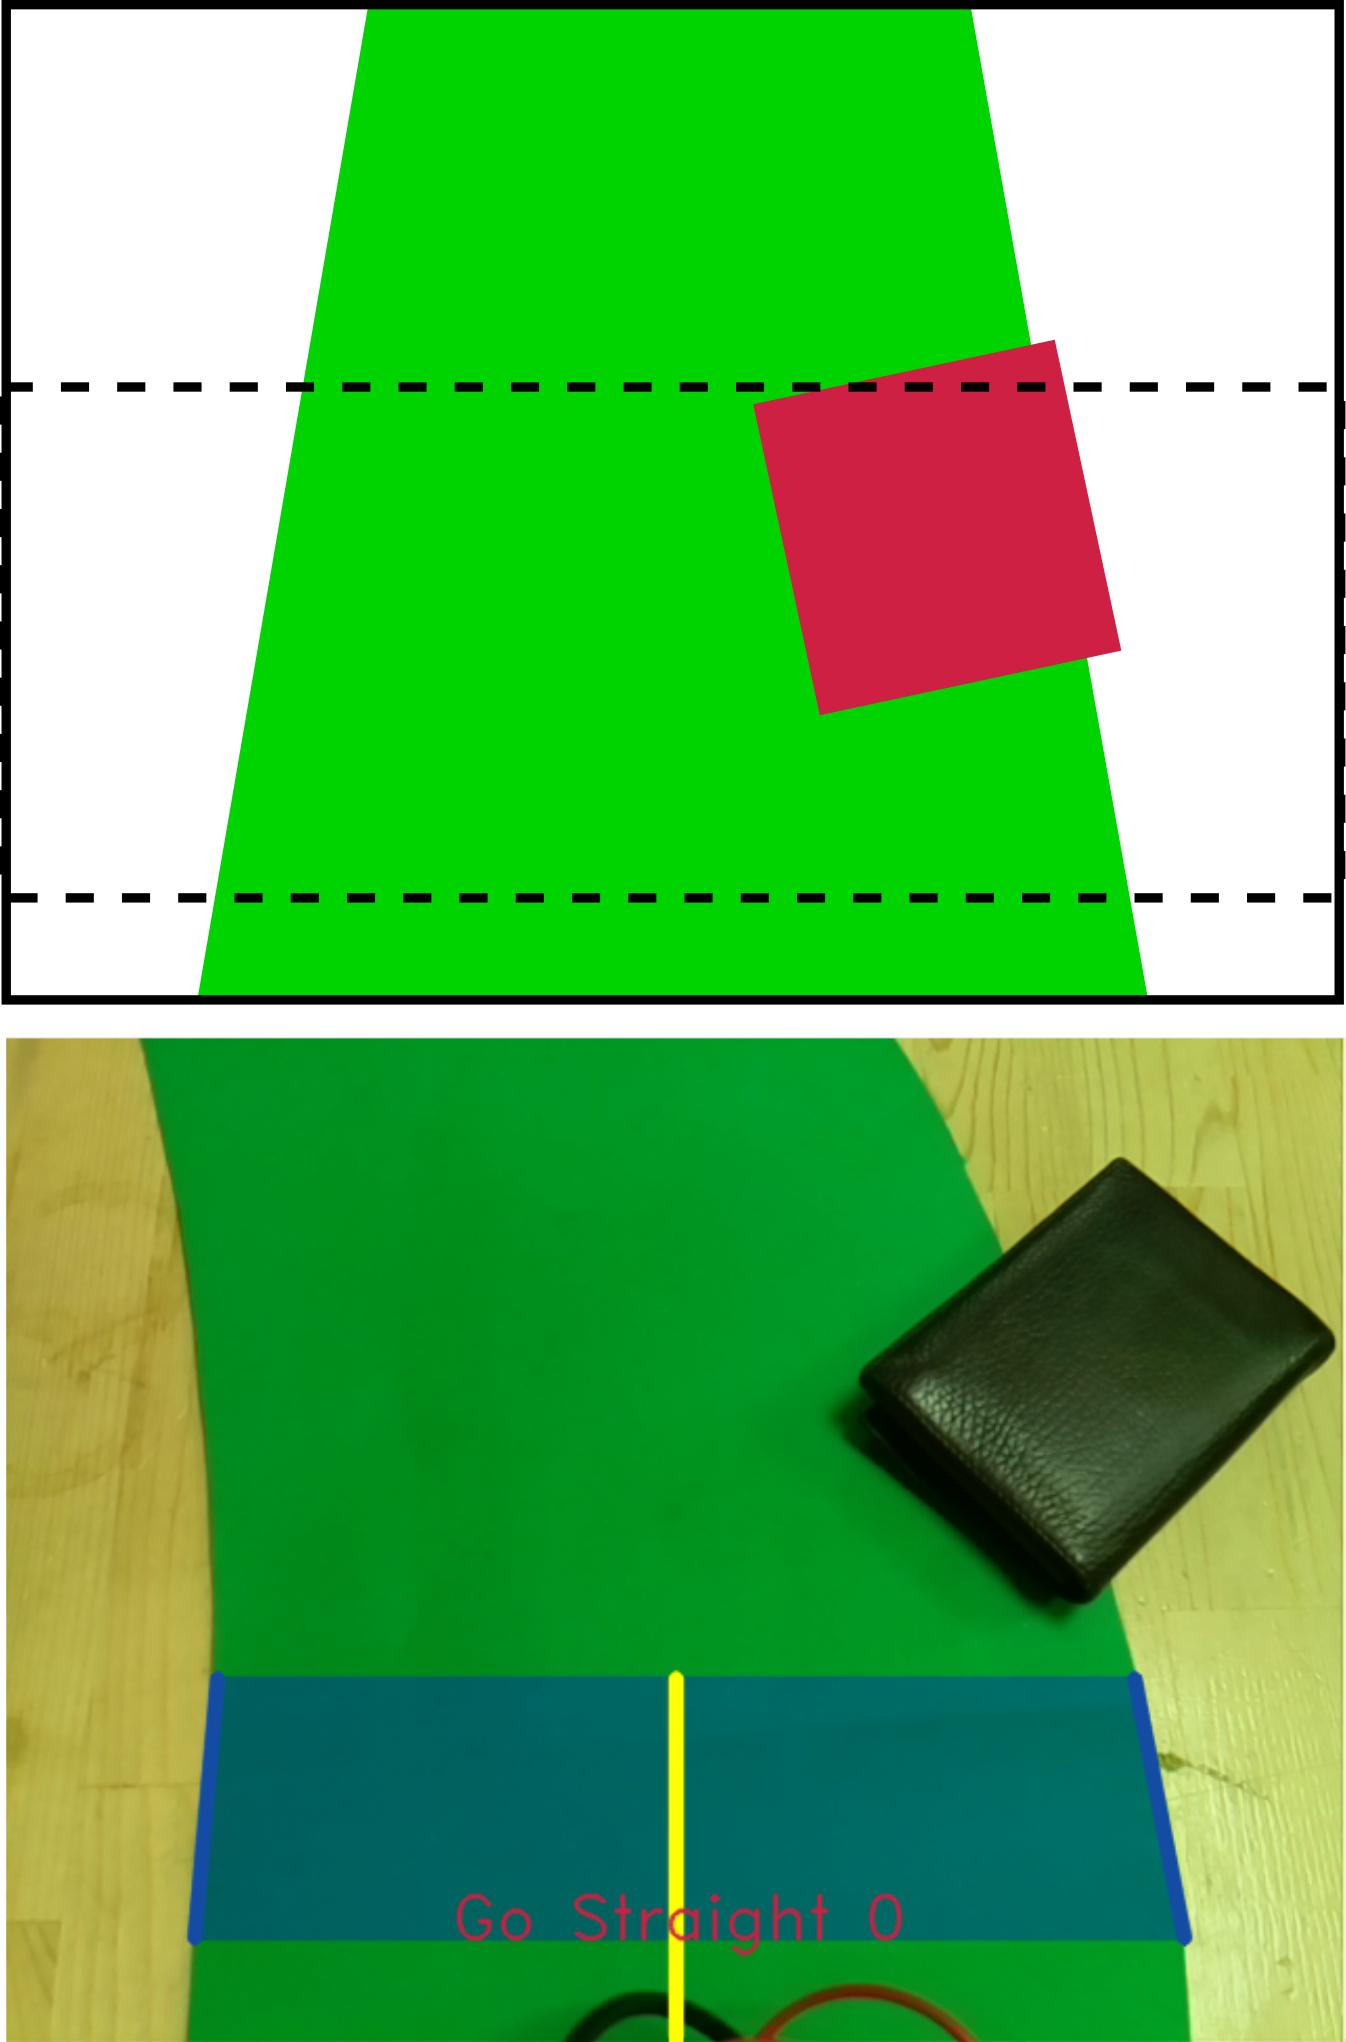
\includegraphics[width=0.30\unitlength]{images/path_images/down_3}

\caption{\label{fig:dataP_down_3} Obstacle is at the End of the Path.}

\end{subfigure}

\caption{\label{fig:dataP_down} A Test Scenario: Downward Inclined Obstacle on the Path. \\ Upper Half: Proposed Tests, Lower Half: Results}

\end{figure}


\begin{figure}[H]

\setlength{\unitlength}{\textwidth} 

\centering

\begin{subfigure}{.31\textwidth}

\centering

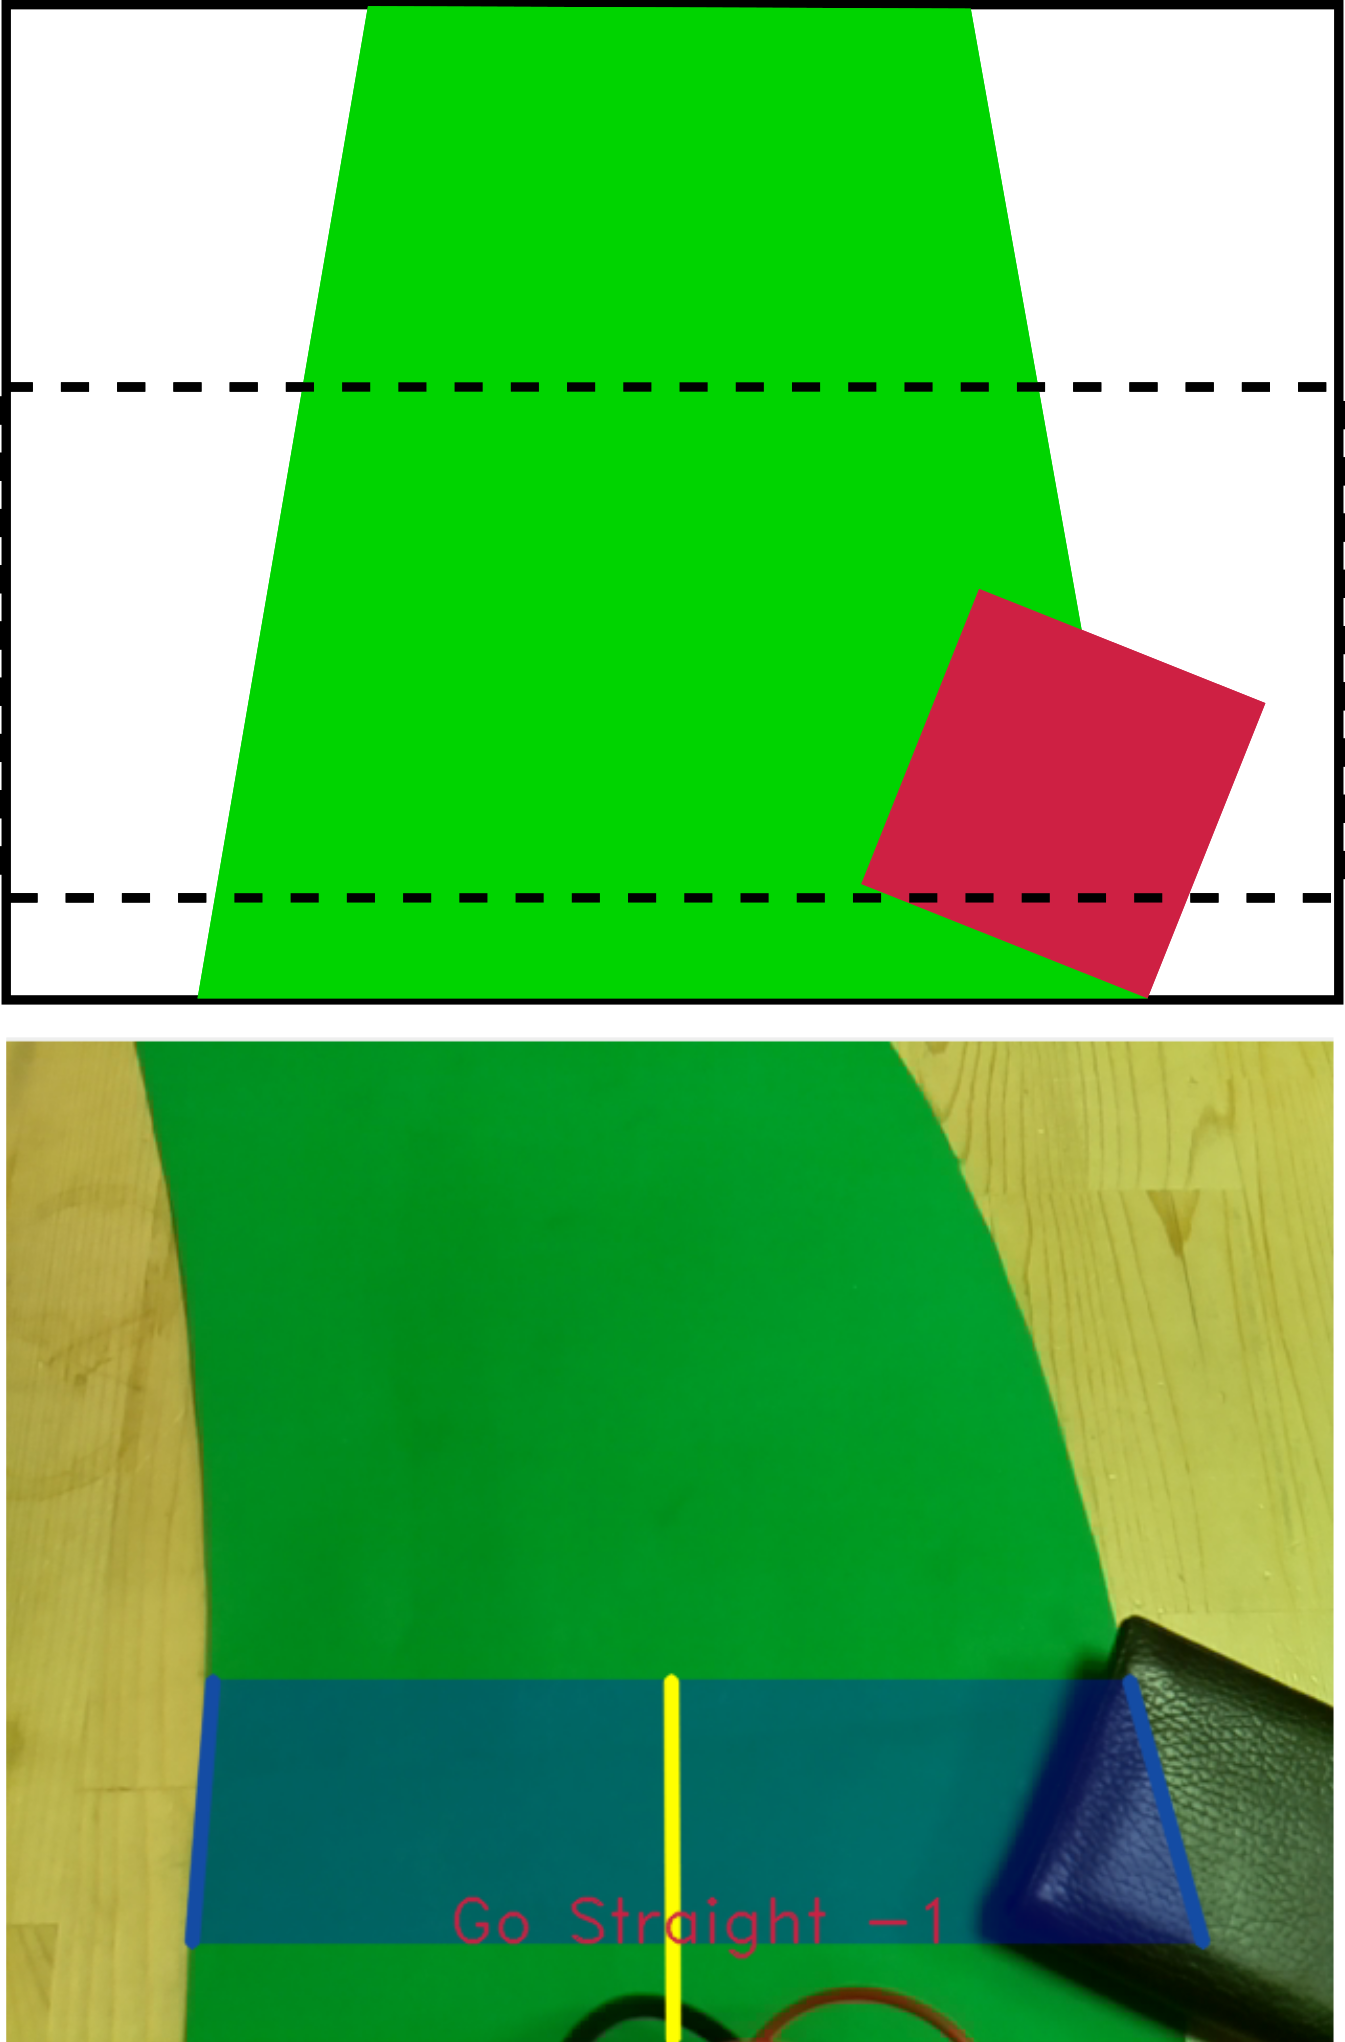
\includegraphics[width=0.30\unitlength]{images/path_images/up_1}

\caption{\label{fig:dataP_up_1} Obstacle is at the Beginning of the Path}

\end{subfigure}%
\begin{subfigure}{.31\textwidth}

\centering

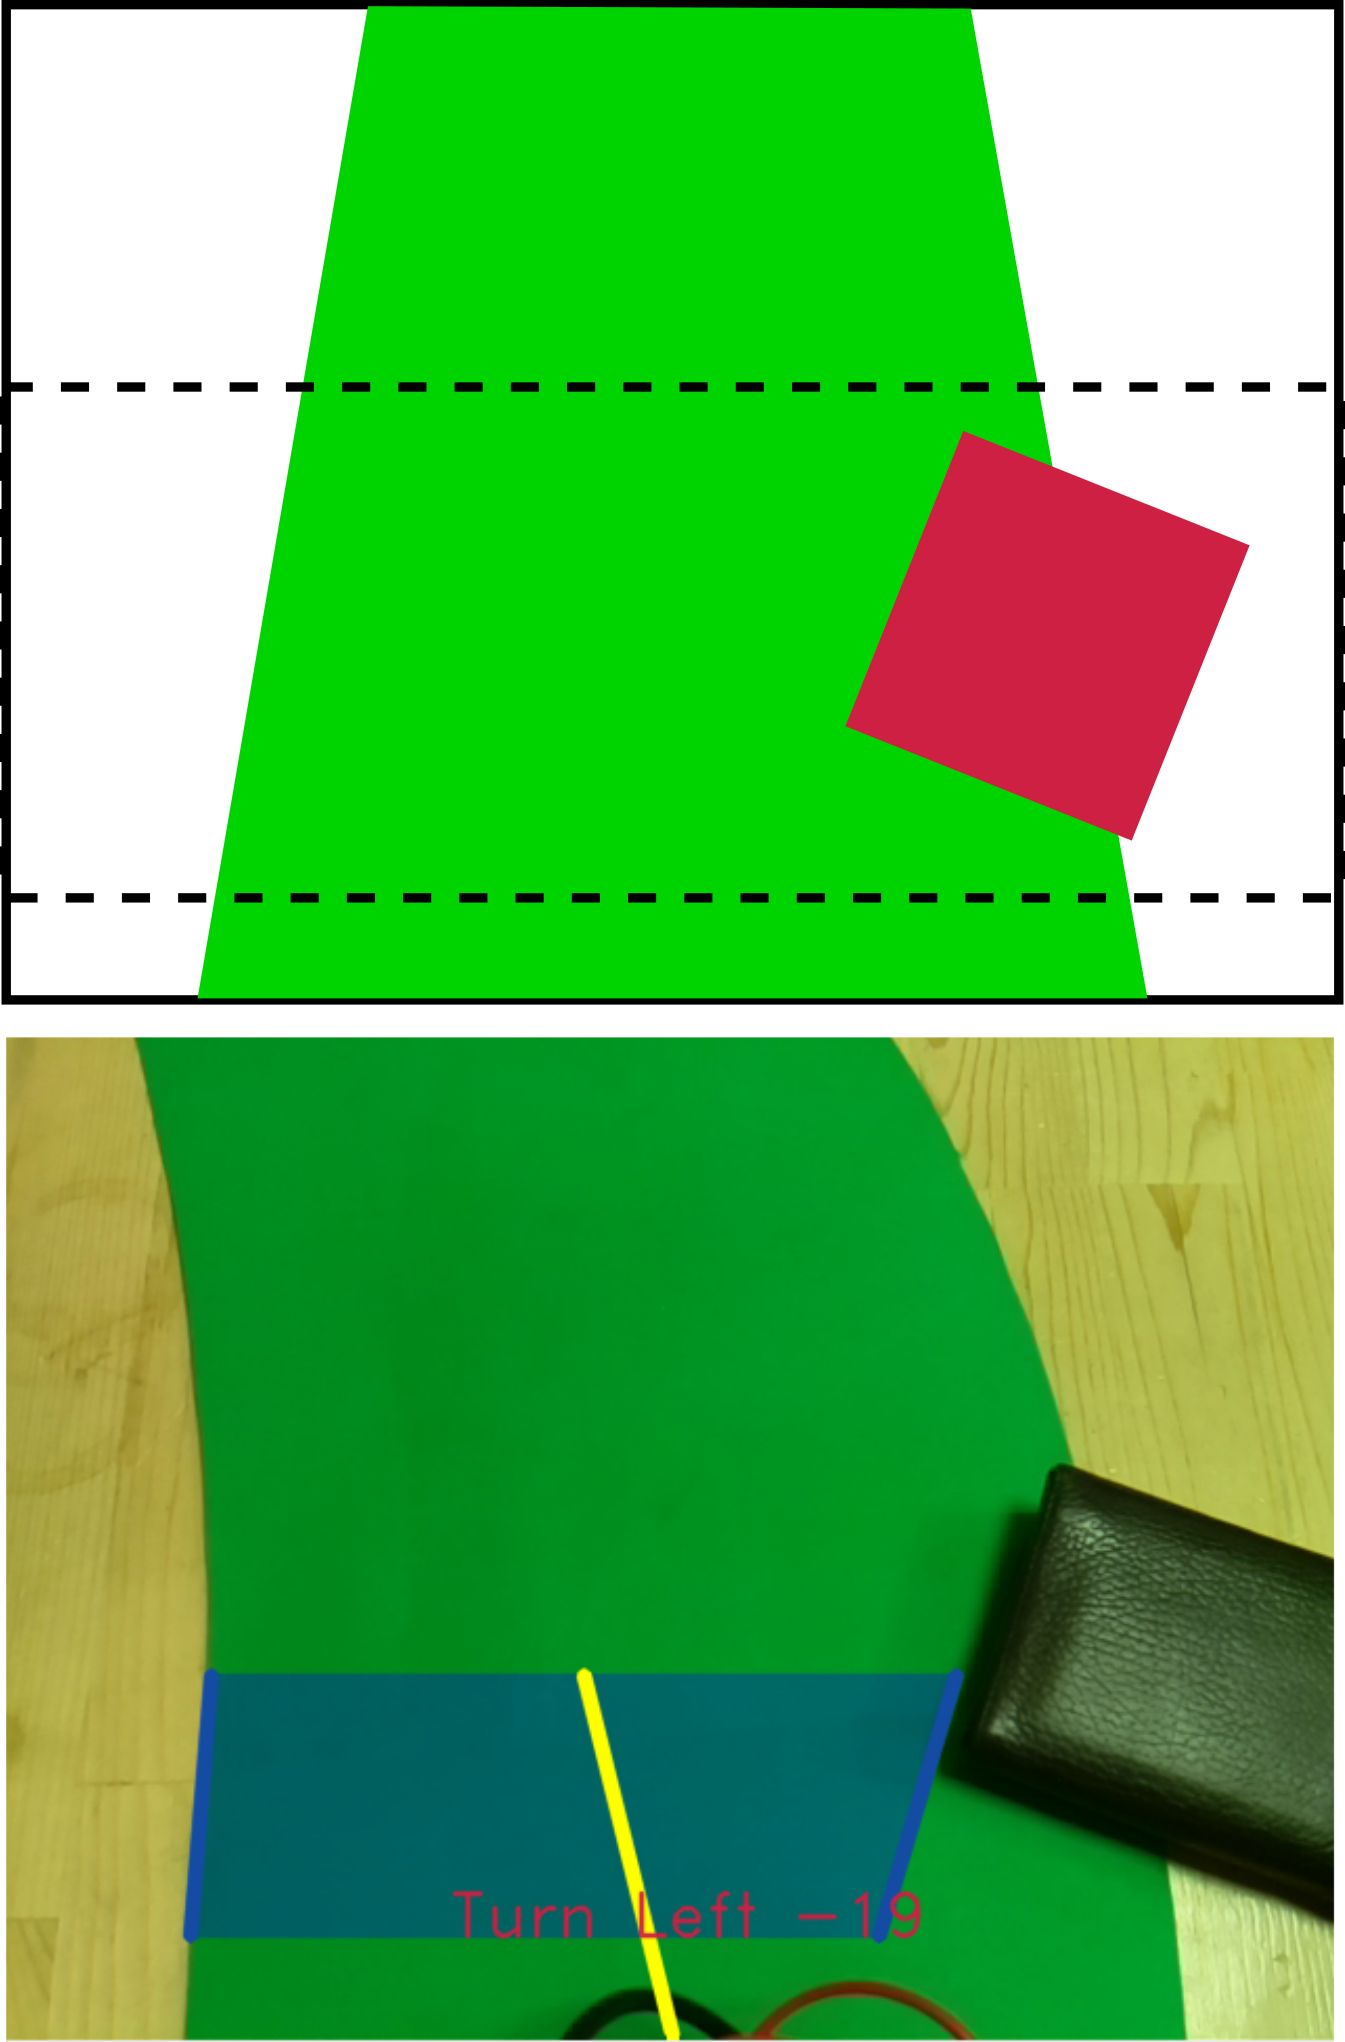
\includegraphics[width=0.30\unitlength]{images/path_images/up_2}

\caption{\label{fig:dataP_up_2} Obstacle is at the Middle of the Path}

\end{subfigure}
\begin{subfigure}{.31\textwidth}

\centering

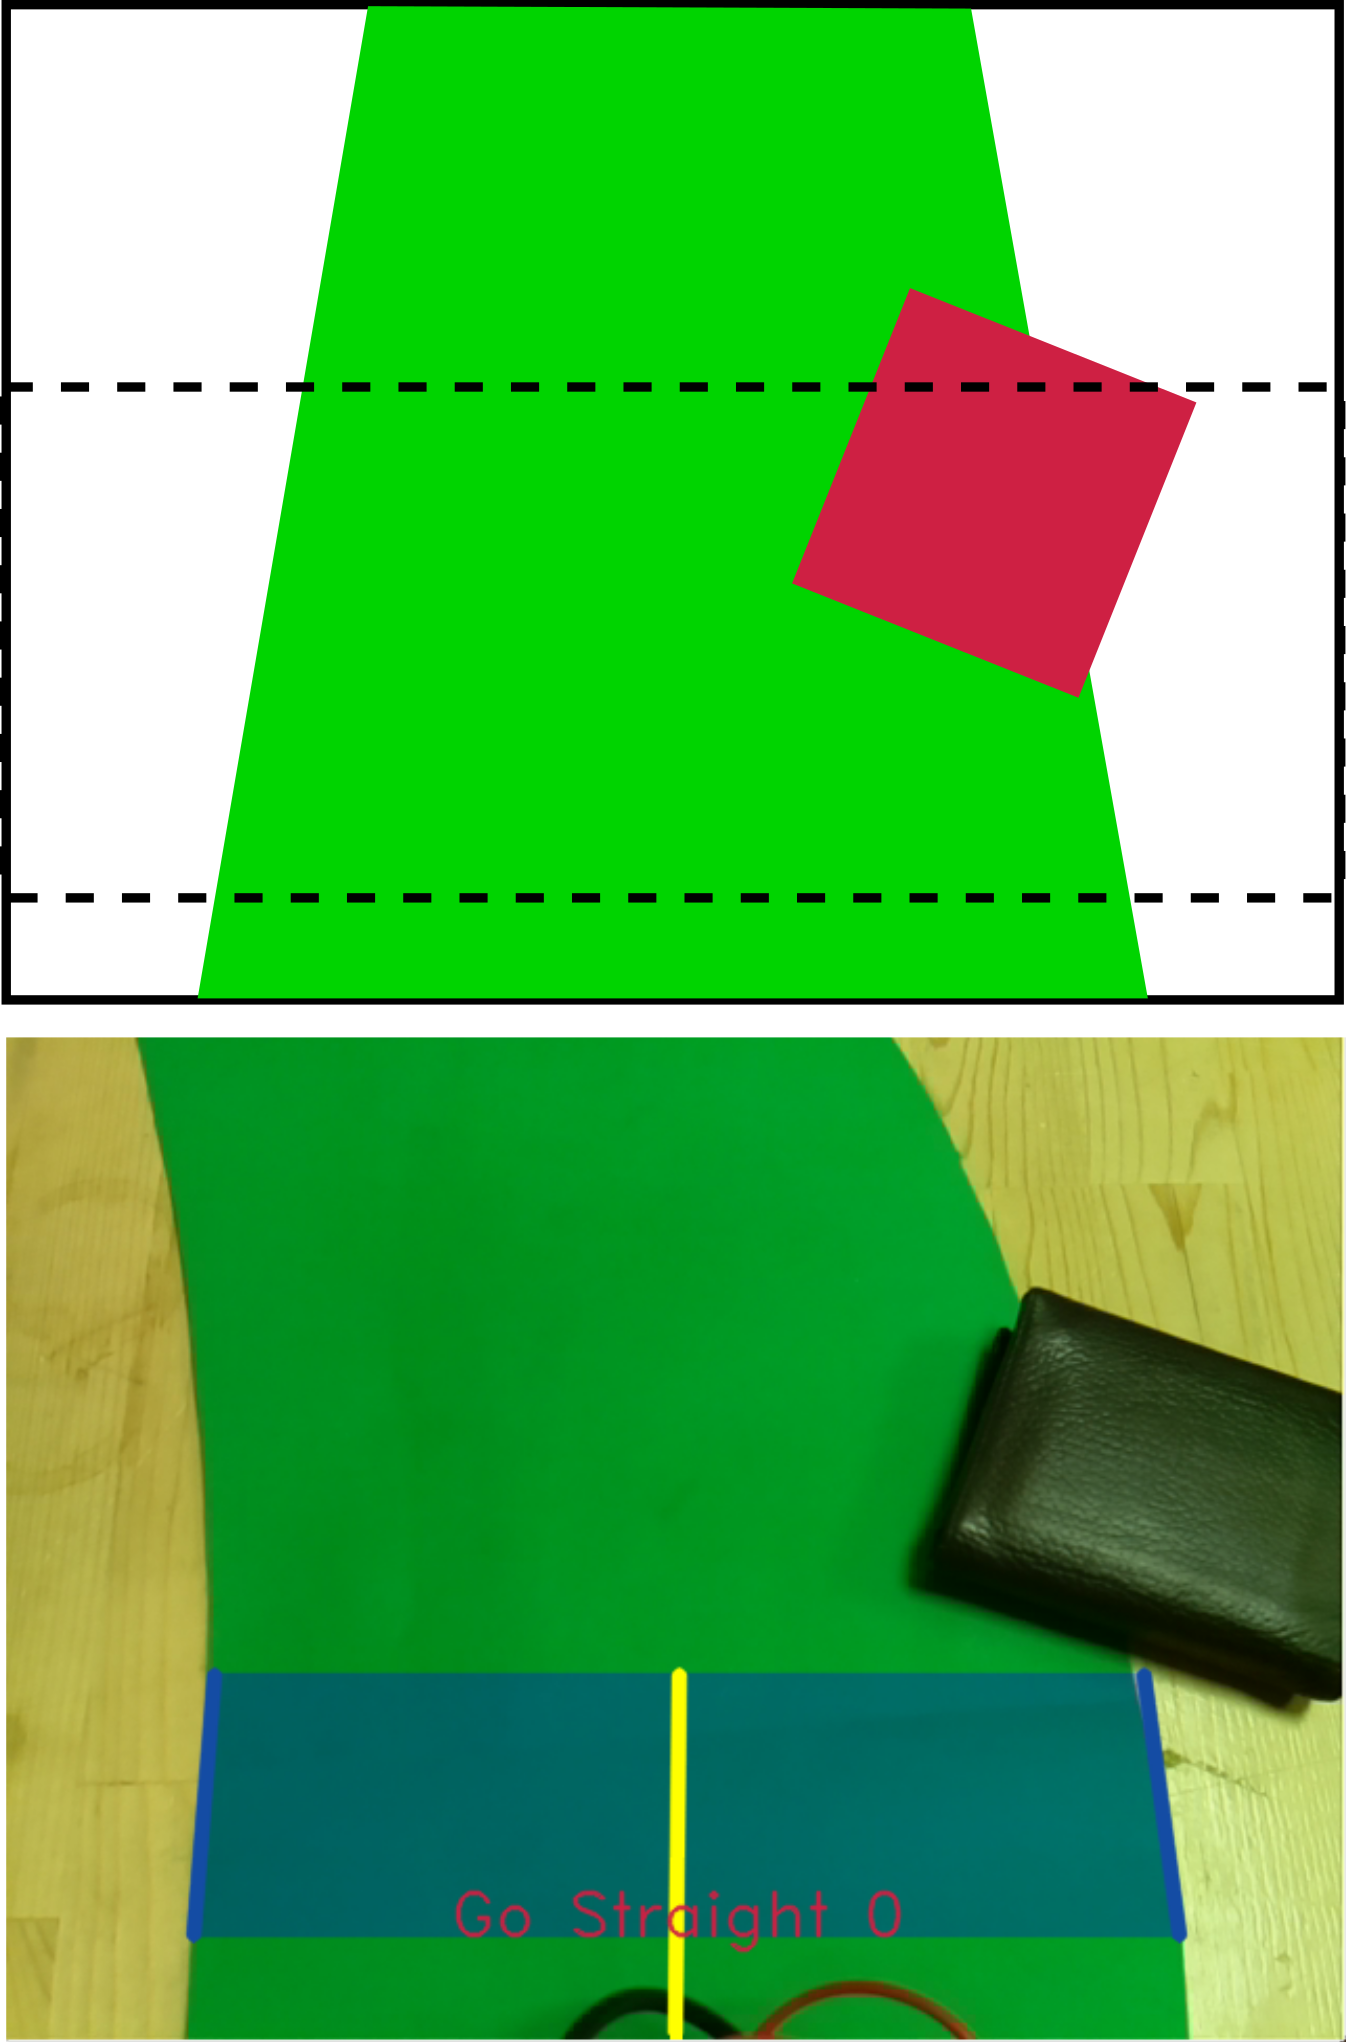
\includegraphics[width=0.30\unitlength]{images/path_images/up_3}

\caption{\label{fig:dataP_up_3} Obstacle is at the End of the Path.}

\end{subfigure}

\caption{\label{fig:dataP_up} A Test Scenario: Upward Inclined Obstacle on the Path. \\ Upper Half: Proposed Tests, Lower Half: Results}

\end{figure}


\begin{figure}[H]

\setlength{\unitlength}{\textwidth} 

\centering

\begin{subfigure}{.31\textwidth}

\centering

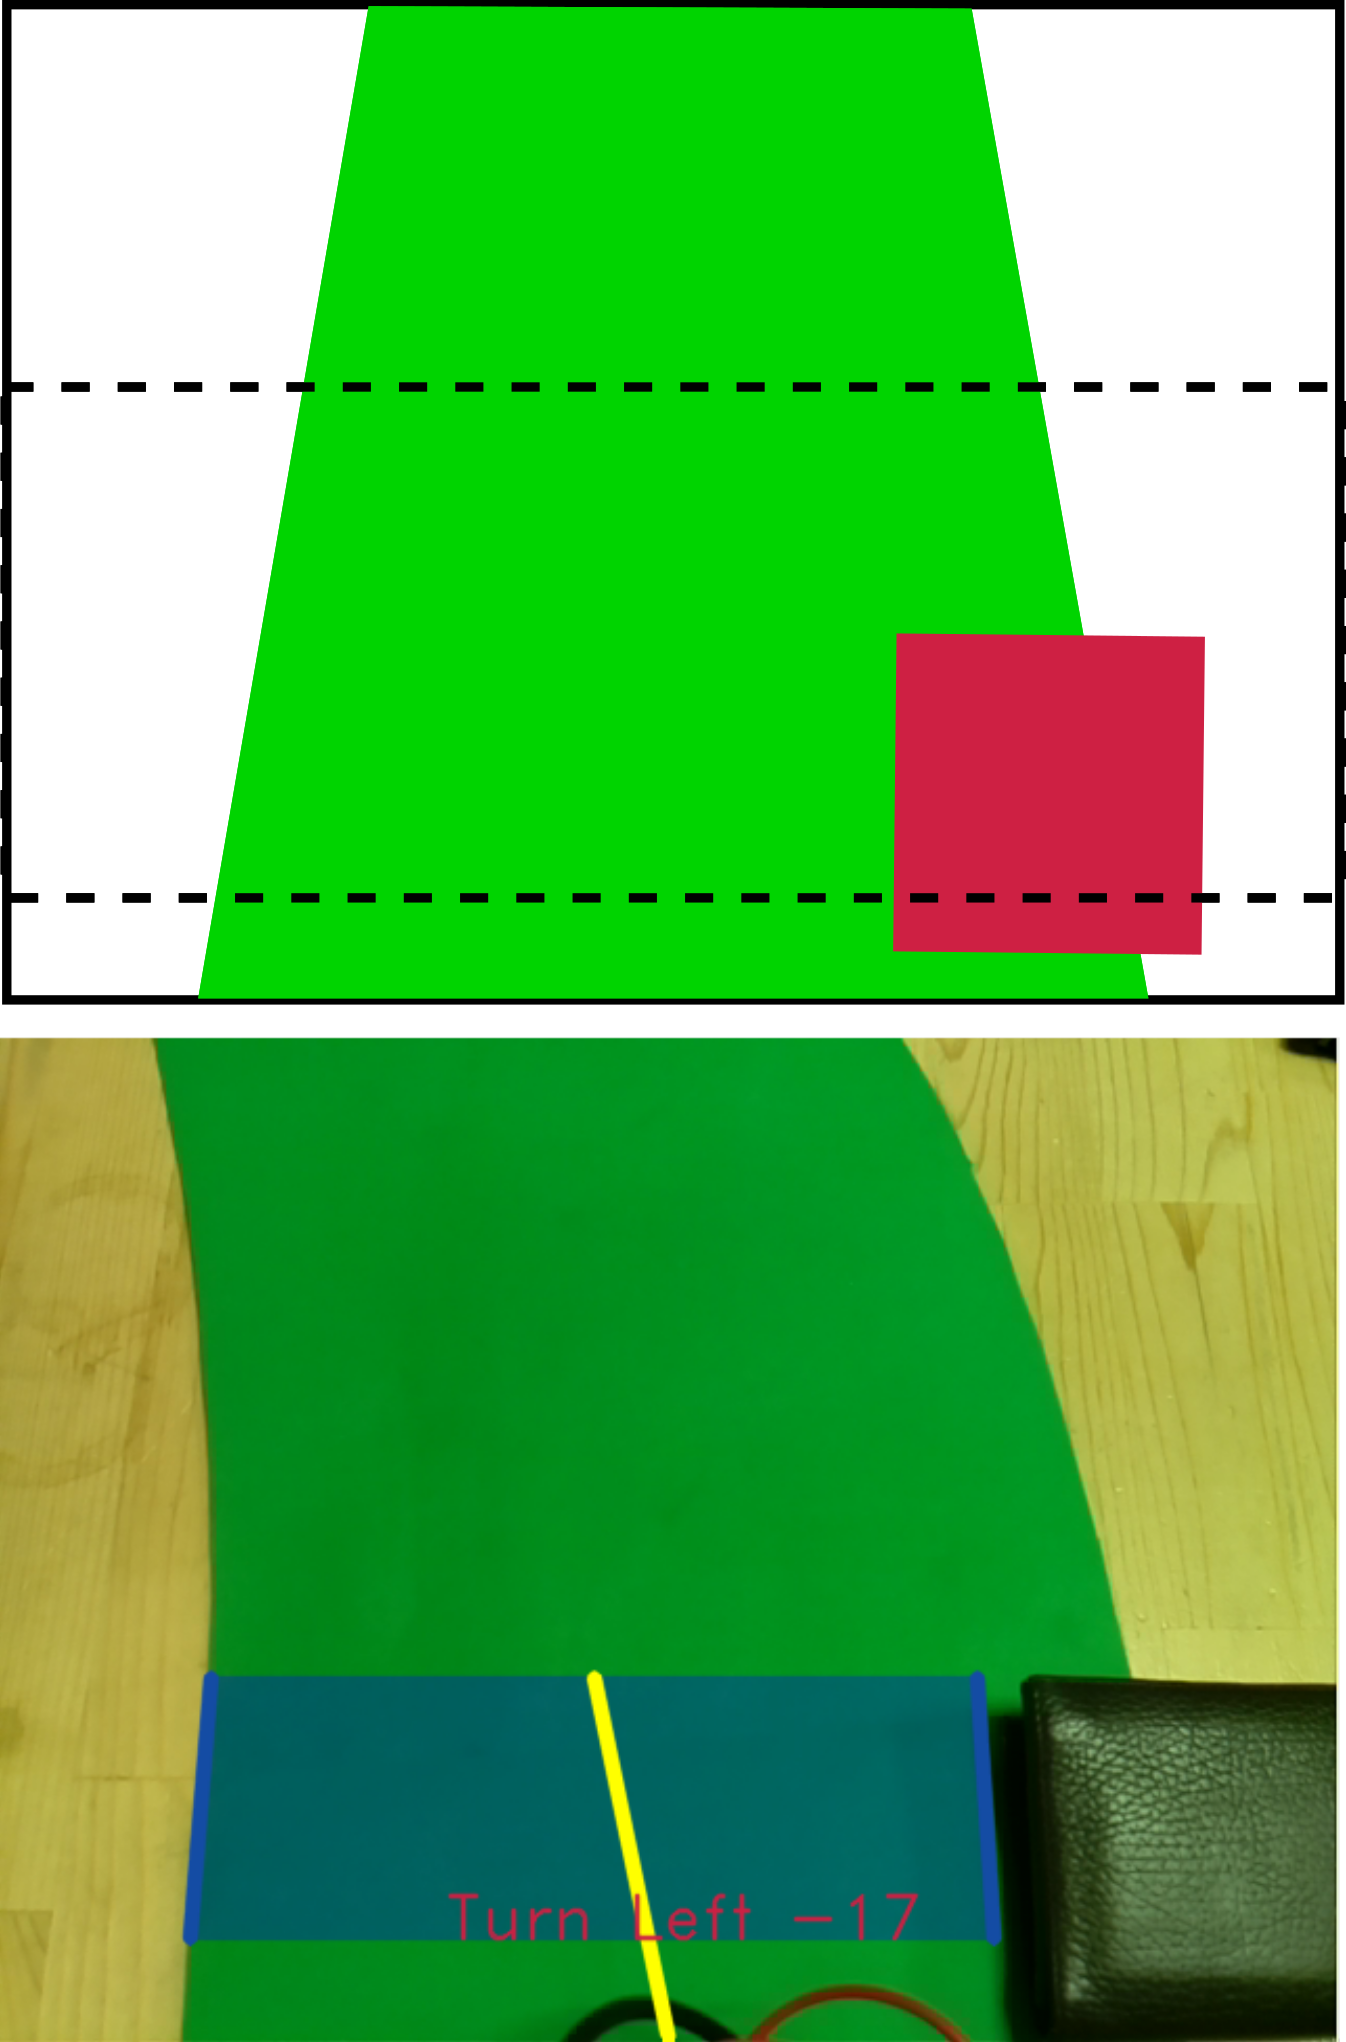
\includegraphics[width=0.30\unitlength]{images/path_images/par_1}

\caption{\label{fig:dataP_par_1} Obstacle is at the Beginning of the Path}

\end{subfigure}%
\begin{subfigure}{.31\textwidth}

\centering

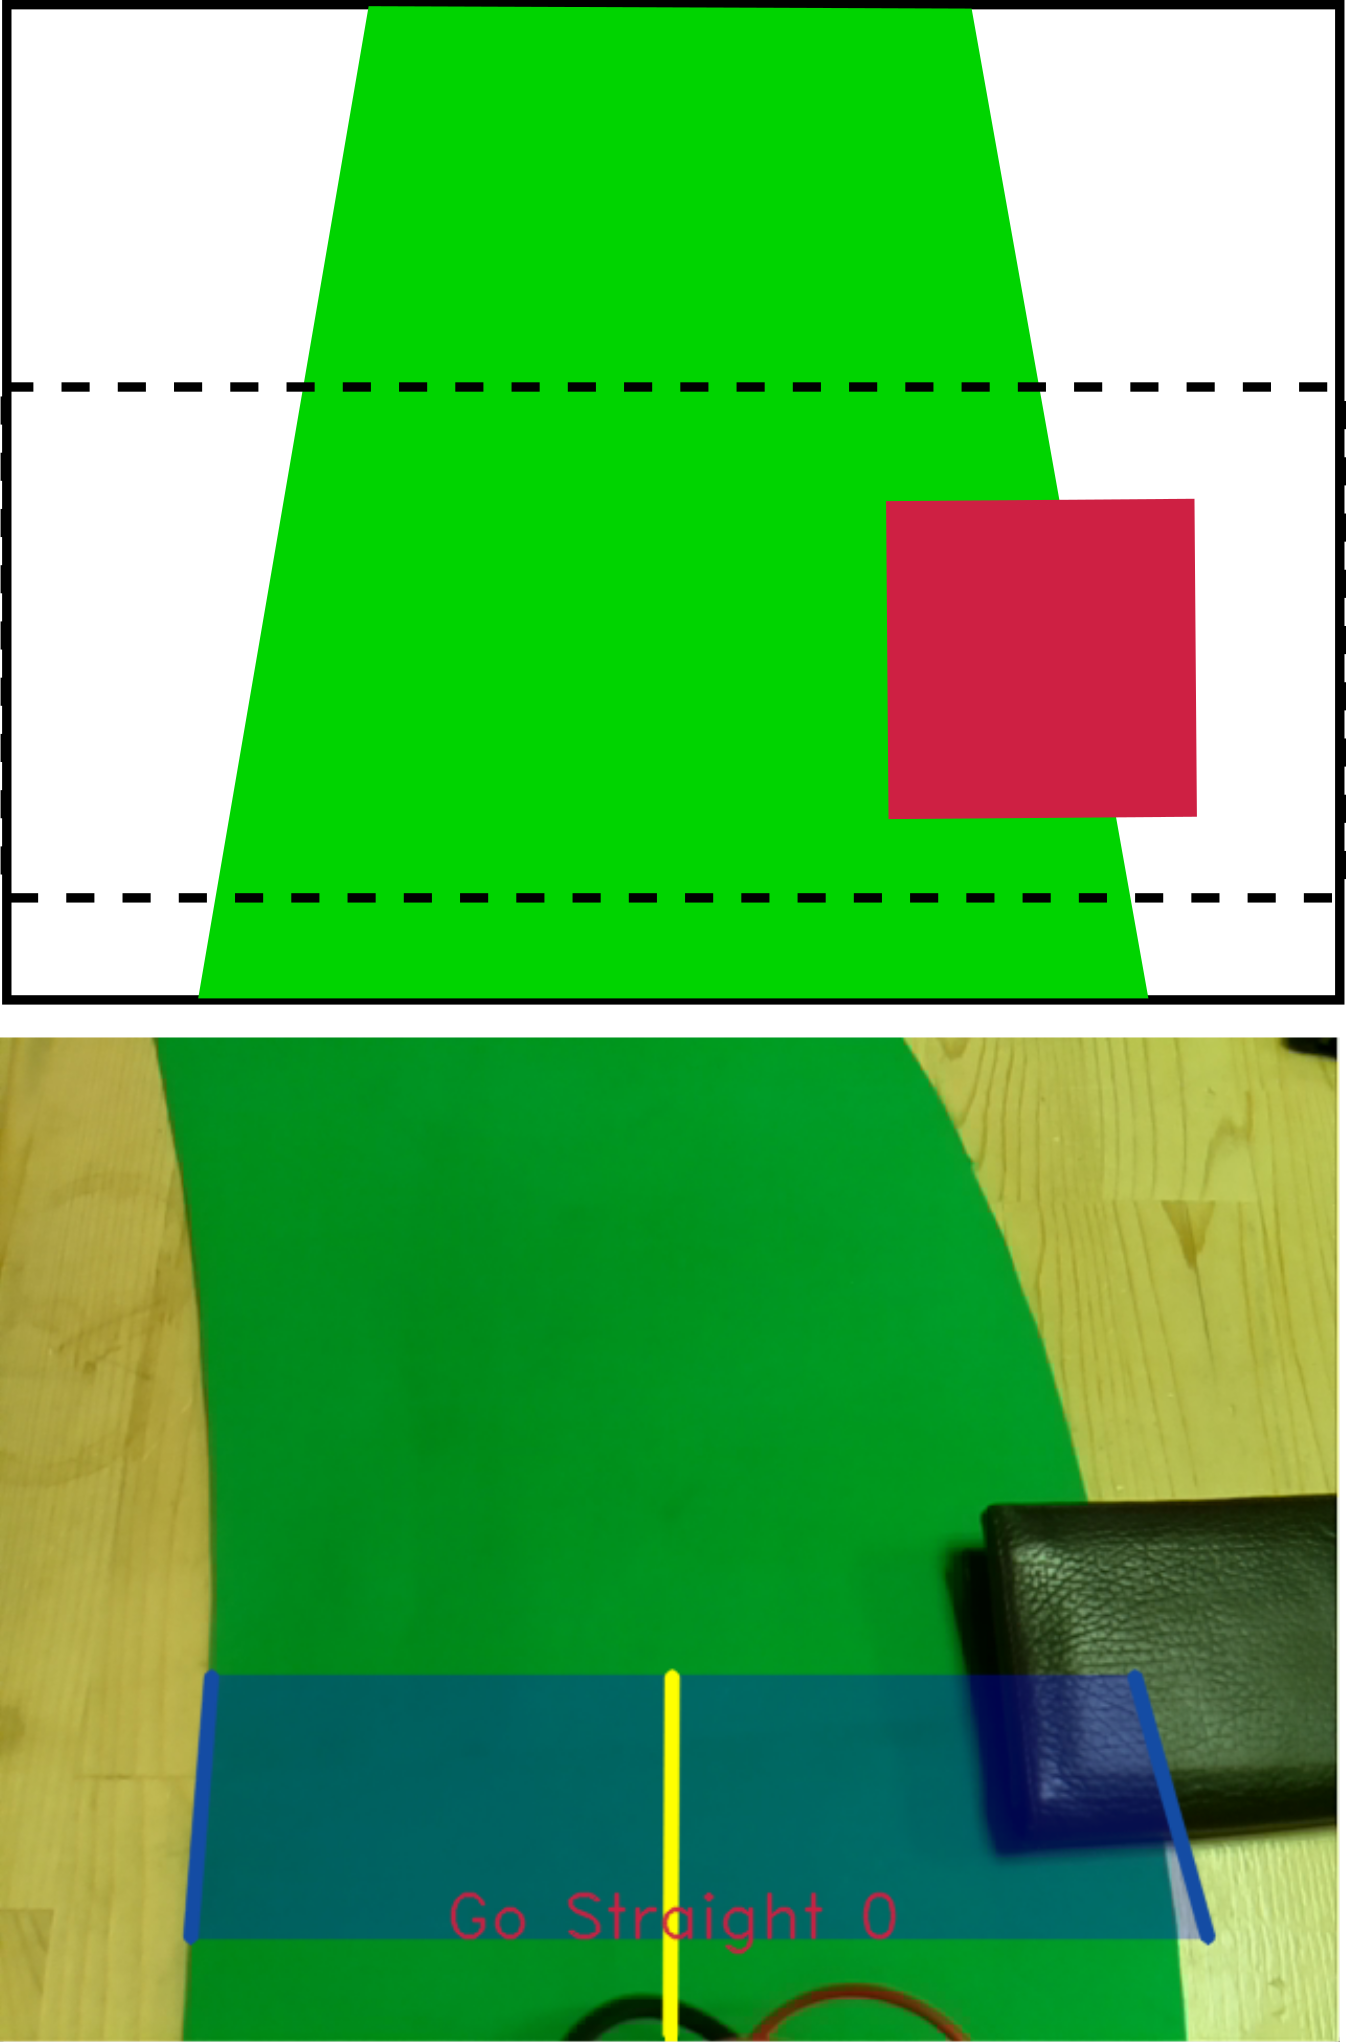
\includegraphics[width=0.30\unitlength]{images/path_images/par_2}

\caption{\label{fig:dataP_par_2} Obstacle is at the Middle of the Path}

\end{subfigure}
\begin{subfigure}{.31\textwidth}

\centering

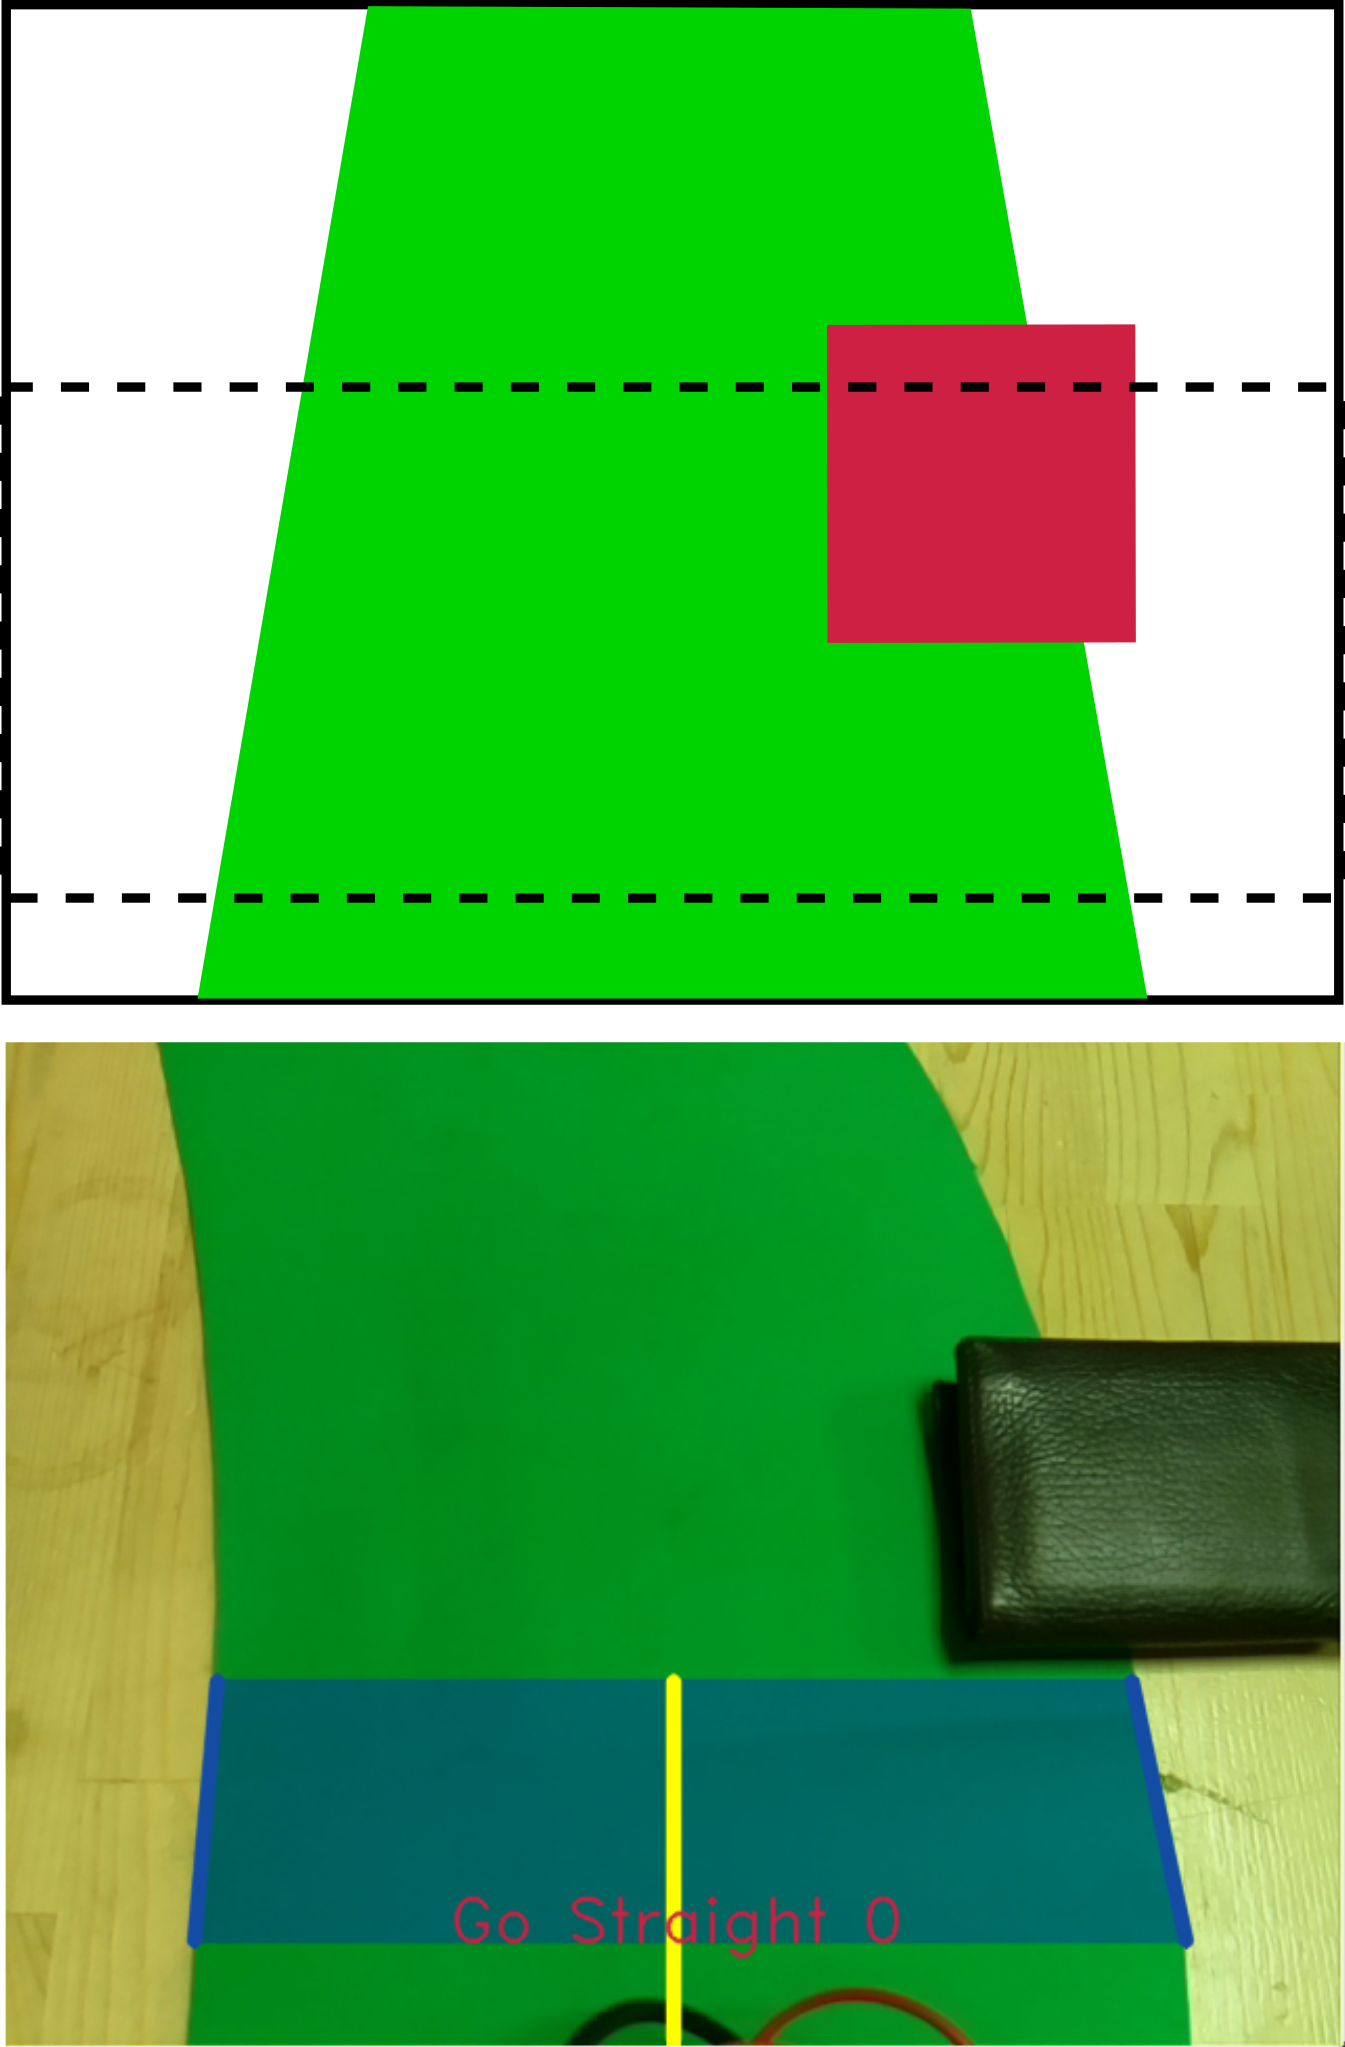
\includegraphics[width=0.30\unitlength]{images/path_images/par_3}

\caption{\label{fig:dataP_par_3} Obstacle is at the End of the Path.}

\end{subfigure}

\caption{\label{fig:dataP_par} A Test Scenario: Parallel Placed Obstacle on the Path. \\ Upper Half: Proposed Tests, Lower Half: Results}

\end{figure}		


\begin{figure}[H]

\setlength{\unitlength}{\textwidth} 

\centering

\begin{subfigure}{.31\textwidth}

\centering

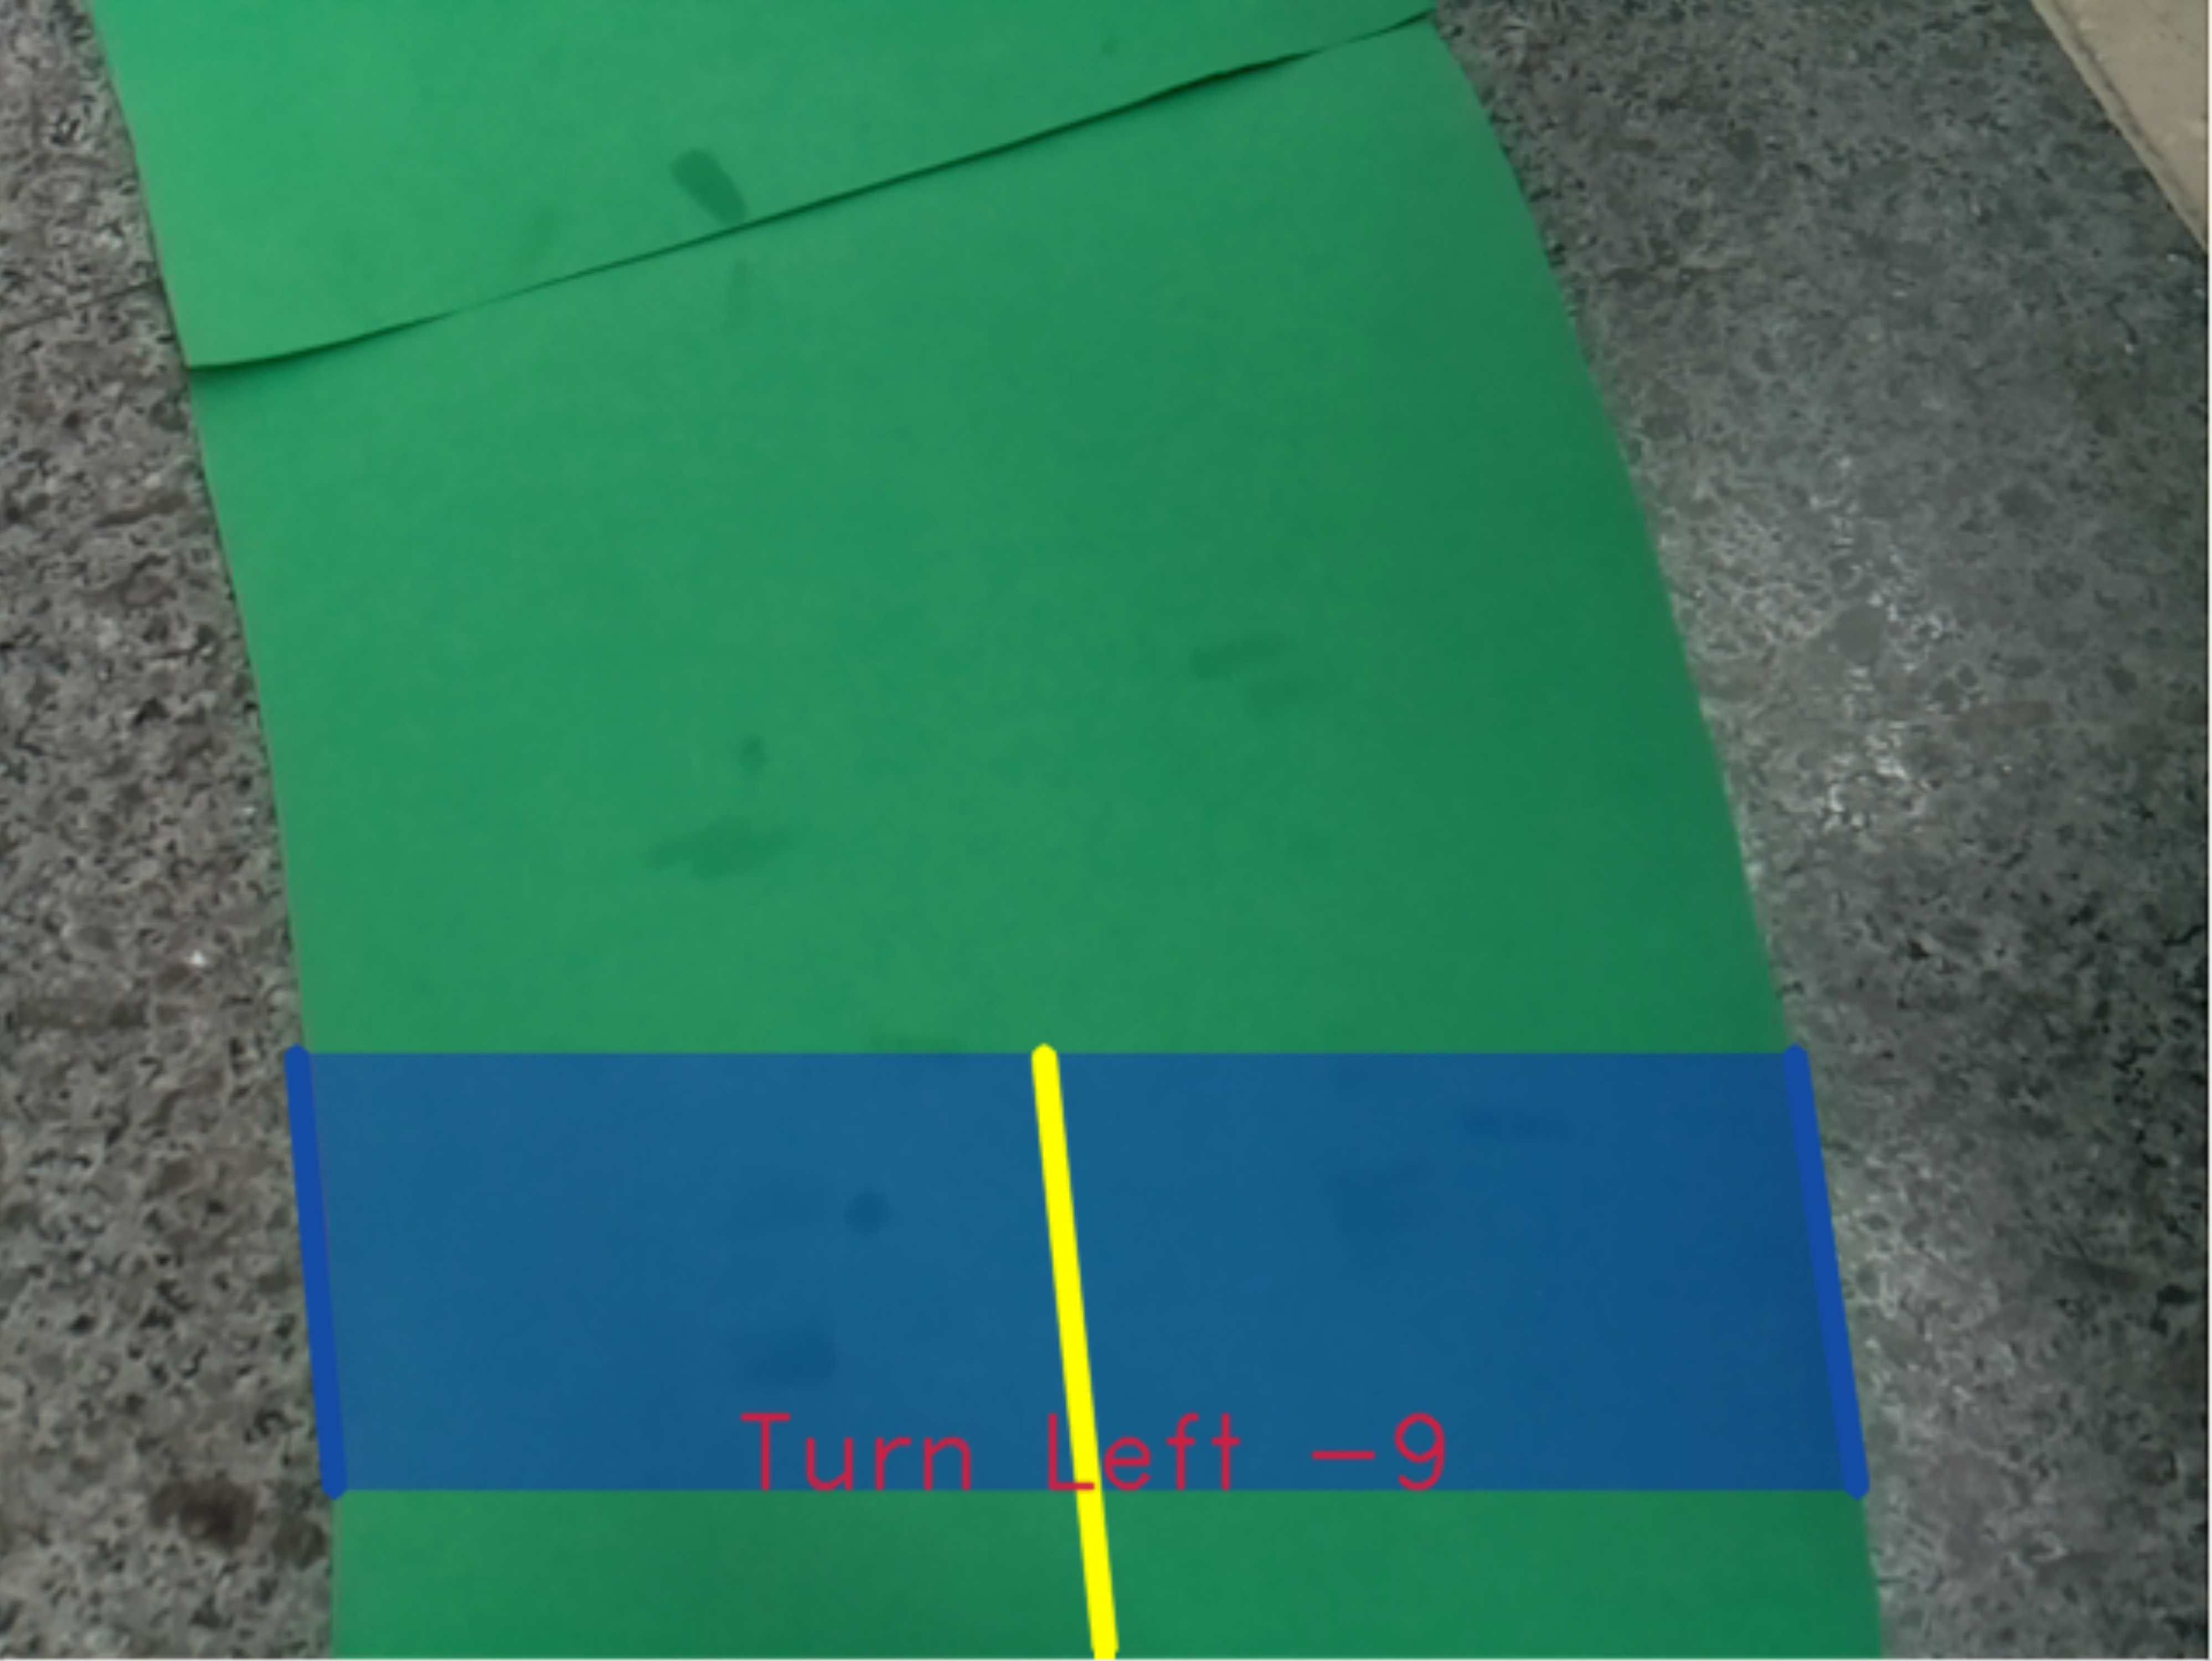
\includegraphics[width=0.30\unitlength]{images/path_images/inside-bb}

\caption{\label{fig:dataP_inside-bb} Path is Placed on Black Marble}

\end{subfigure}%
\begin{subfigure}{.31\textwidth}

\centering

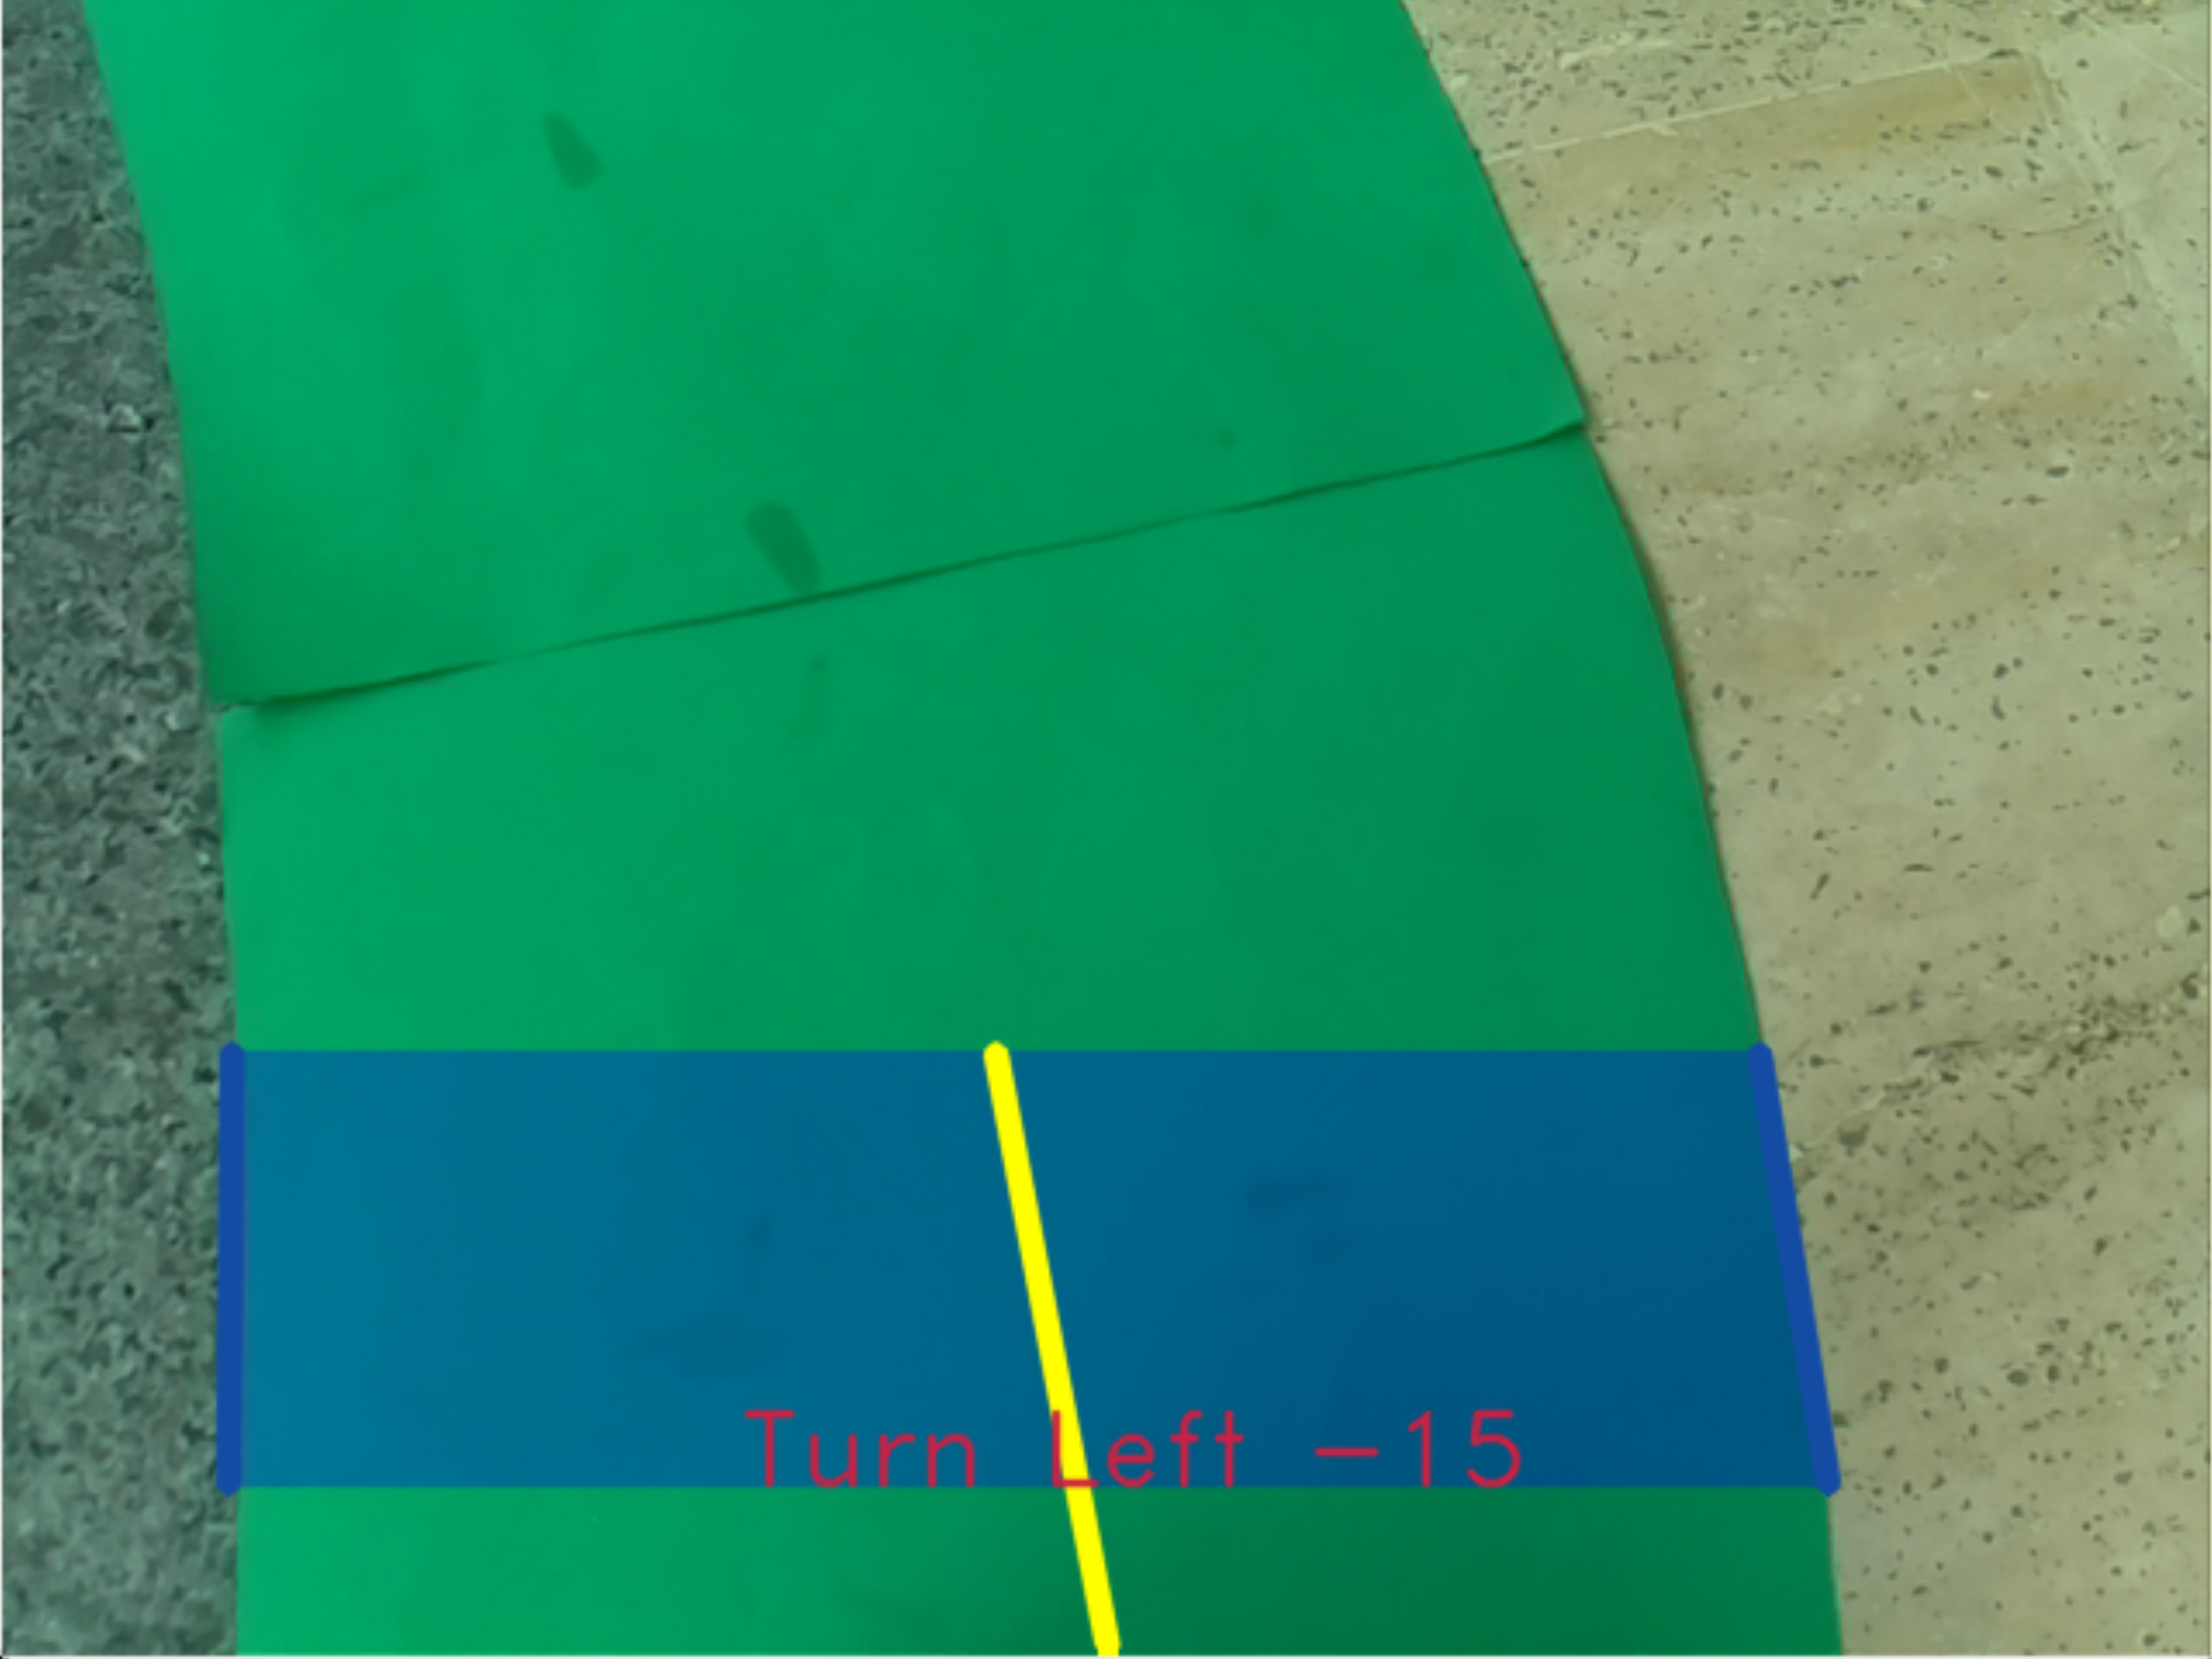
\includegraphics[width=0.30\unitlength]{images/path_images/inside-bw}

\caption{\label{fig:dataP_inside-bw} Path is Placed on Black and White Marble}

\end{subfigure}
\begin{subfigure}{.31\textwidth}

\centering

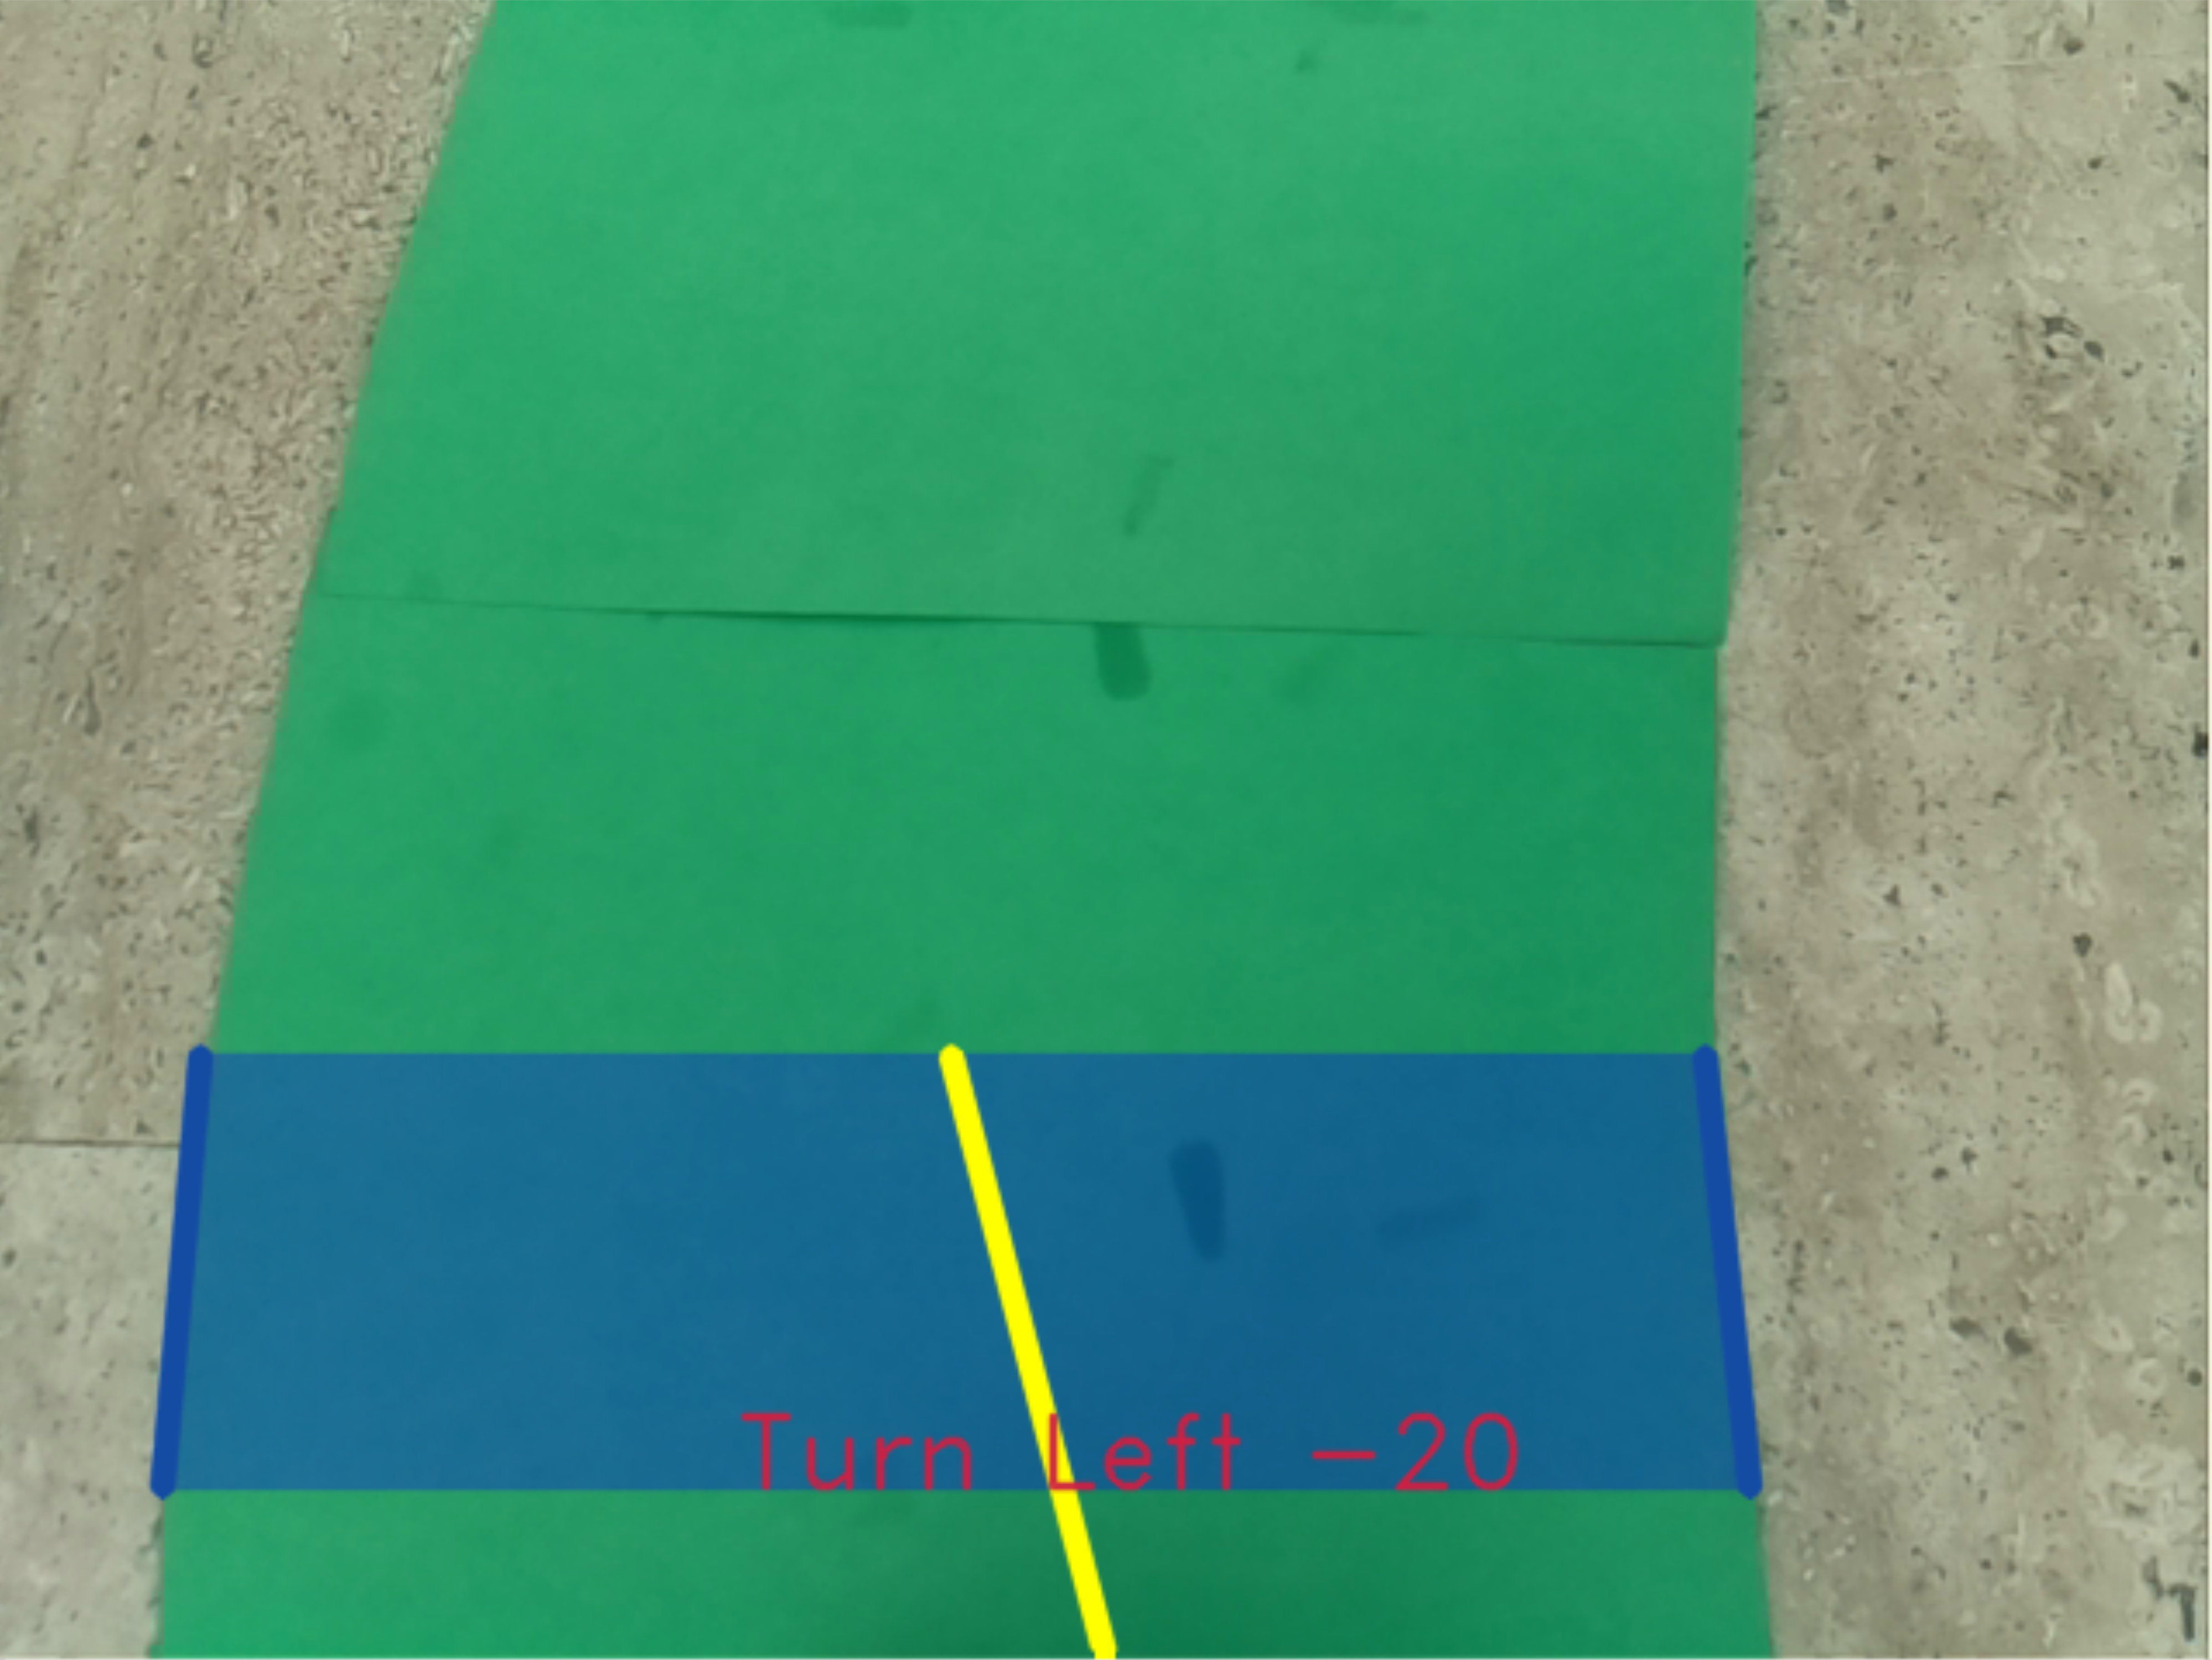
\includegraphics[width=0.30\unitlength]{images/path_images/inside-ww}

\caption{\label{fig:dataP_inside-ww} Path is Placed on White Marble}

\end{subfigure}

\caption{\label{fig:dataP_inside} A Test Scenario Results: KKM Indoor Path Detection}

\end{figure}


\begin{figure}[H]

\setlength{\unitlength}{\textwidth} 

\centering

\begin{subfigure}{.31\textwidth}

\centering

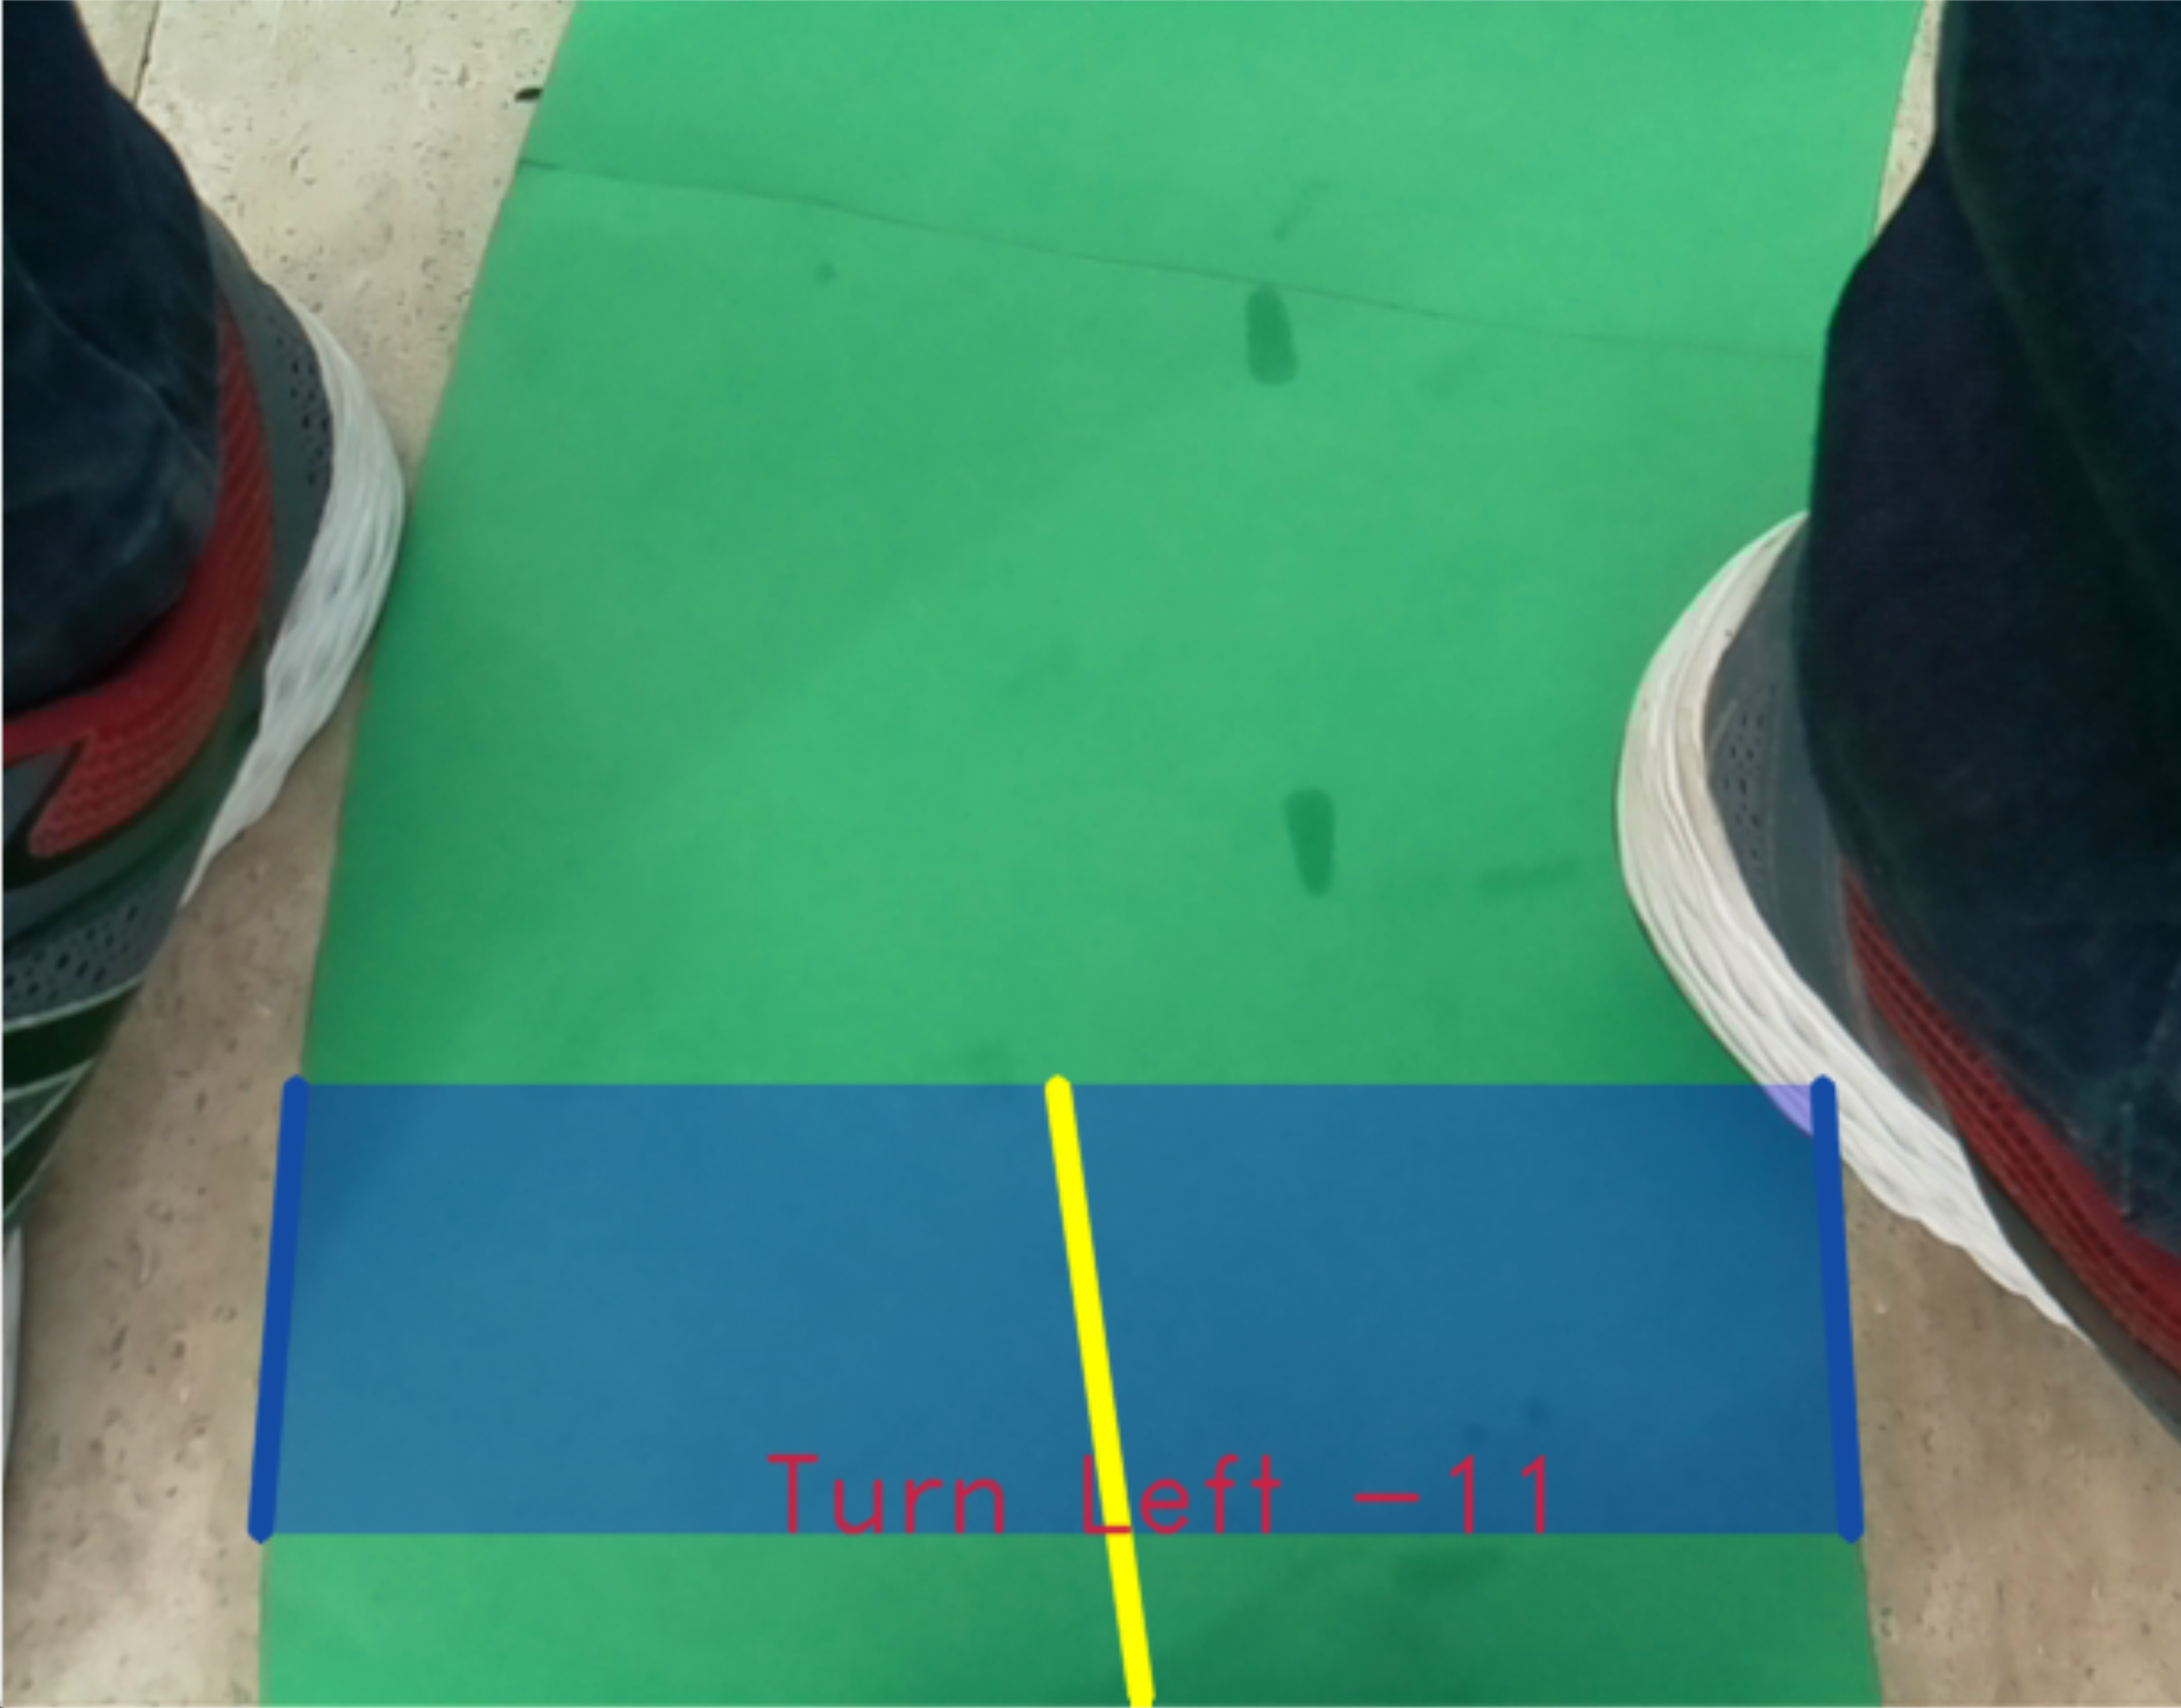
\includegraphics[width=0.30\unitlength]{images/path_images/outsideObs0}

\caption{\label{fig:dataP_outsideObs0} Daylight and Shadow Test-1}

\end{subfigure}%
\begin{subfigure}{.31\textwidth}

\centering

\includegraphics[width=0.30\unitlength]{images/path_images/outsideObs1}

\caption{\label{fig:dataP_outsideObs1} Daylight and Shadow Test-2}

\end{subfigure}
\begin{subfigure}{.31\textwidth}

\centering

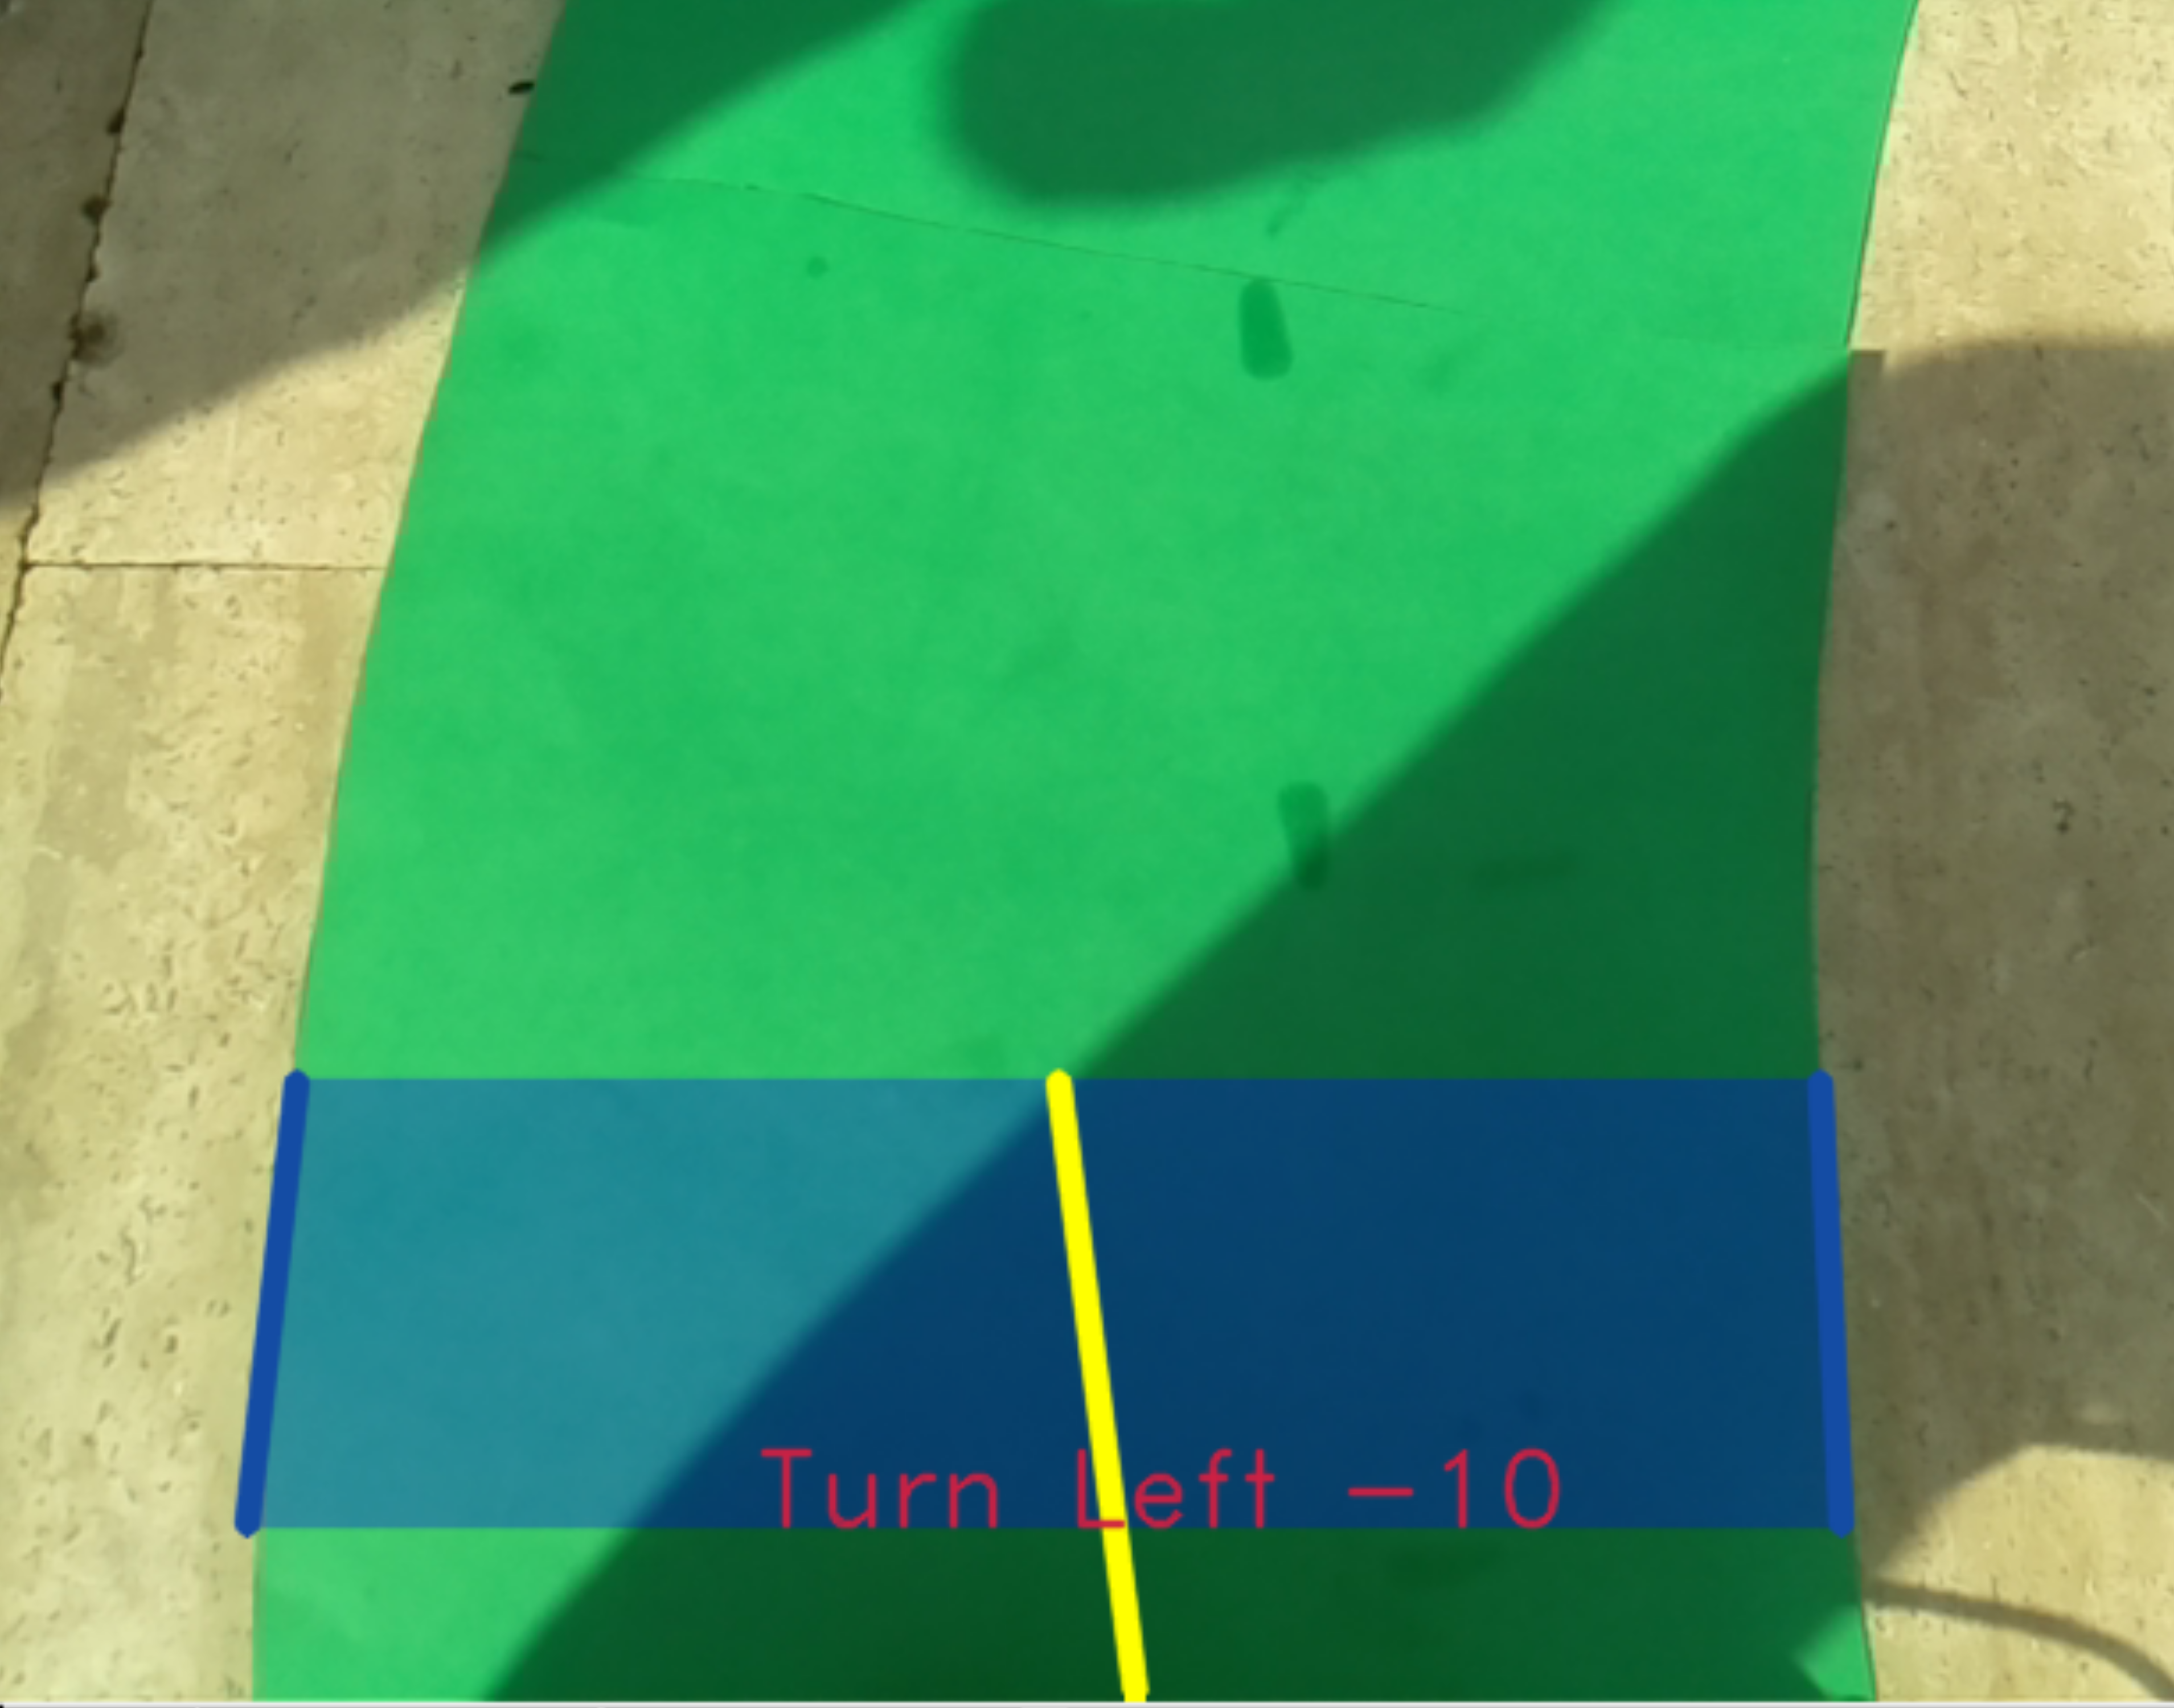
\includegraphics[width=0.30\unitlength]{images/path_images/outsideObs2}

\caption{\label{fig:dataP_outsideObs2} Daylight and Shadow Test-3}

\end{subfigure}

\caption{\label{fig:dataP_outside} A Test Scenario Results: KKM Outdoor Path Detection}

\end{figure}

\begin{figure}[h!]
	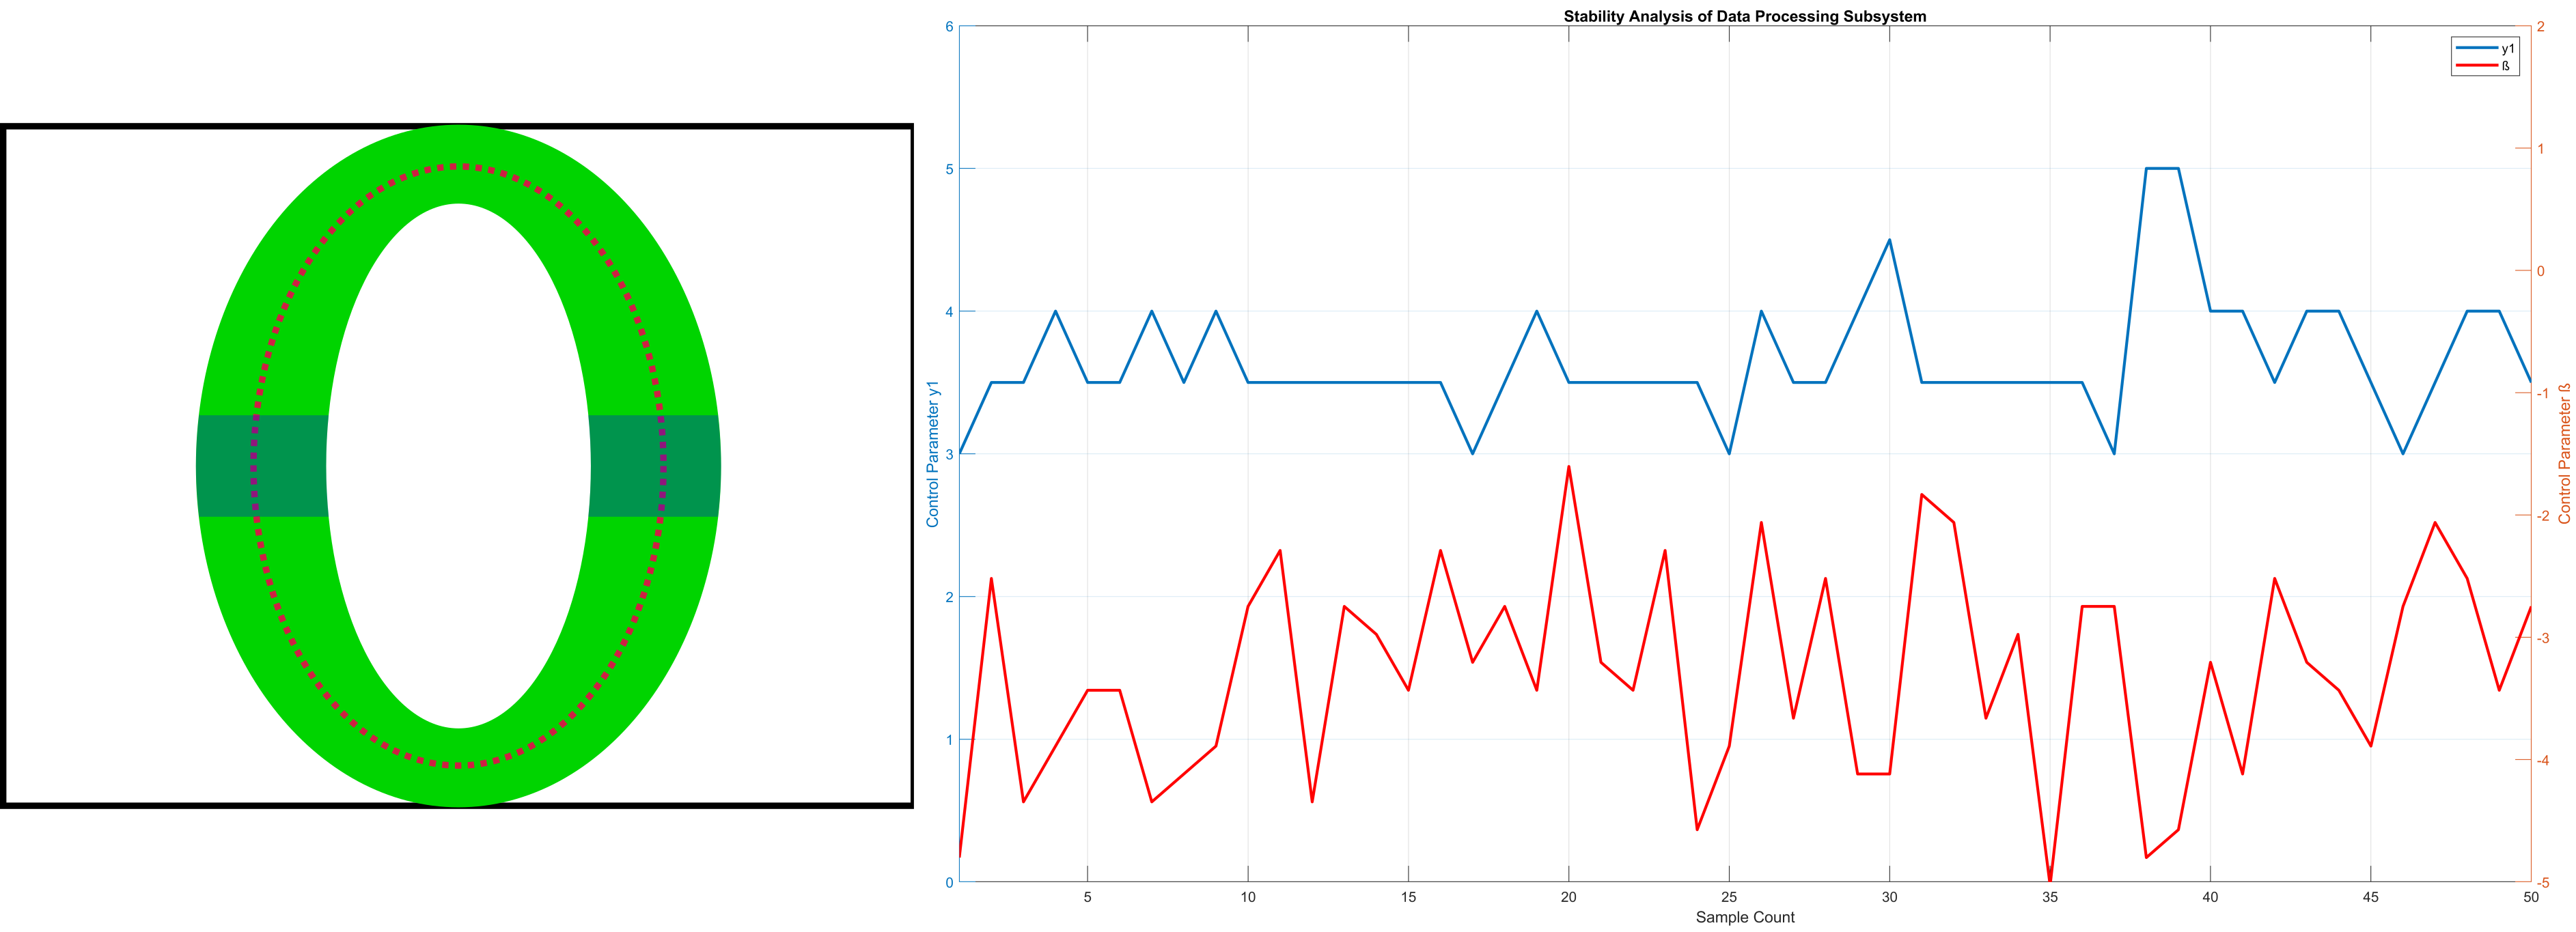
\includegraphics[width=.95\textwidth,center]{images/stabilityTestI}
	\caption{ Left: The Vehicle is placed on Straight Area.\\ Right: The Control Outputs \label{fig:stabilityTestI-dist} }
\end{figure}		

\begin{figure}[h!]
	
	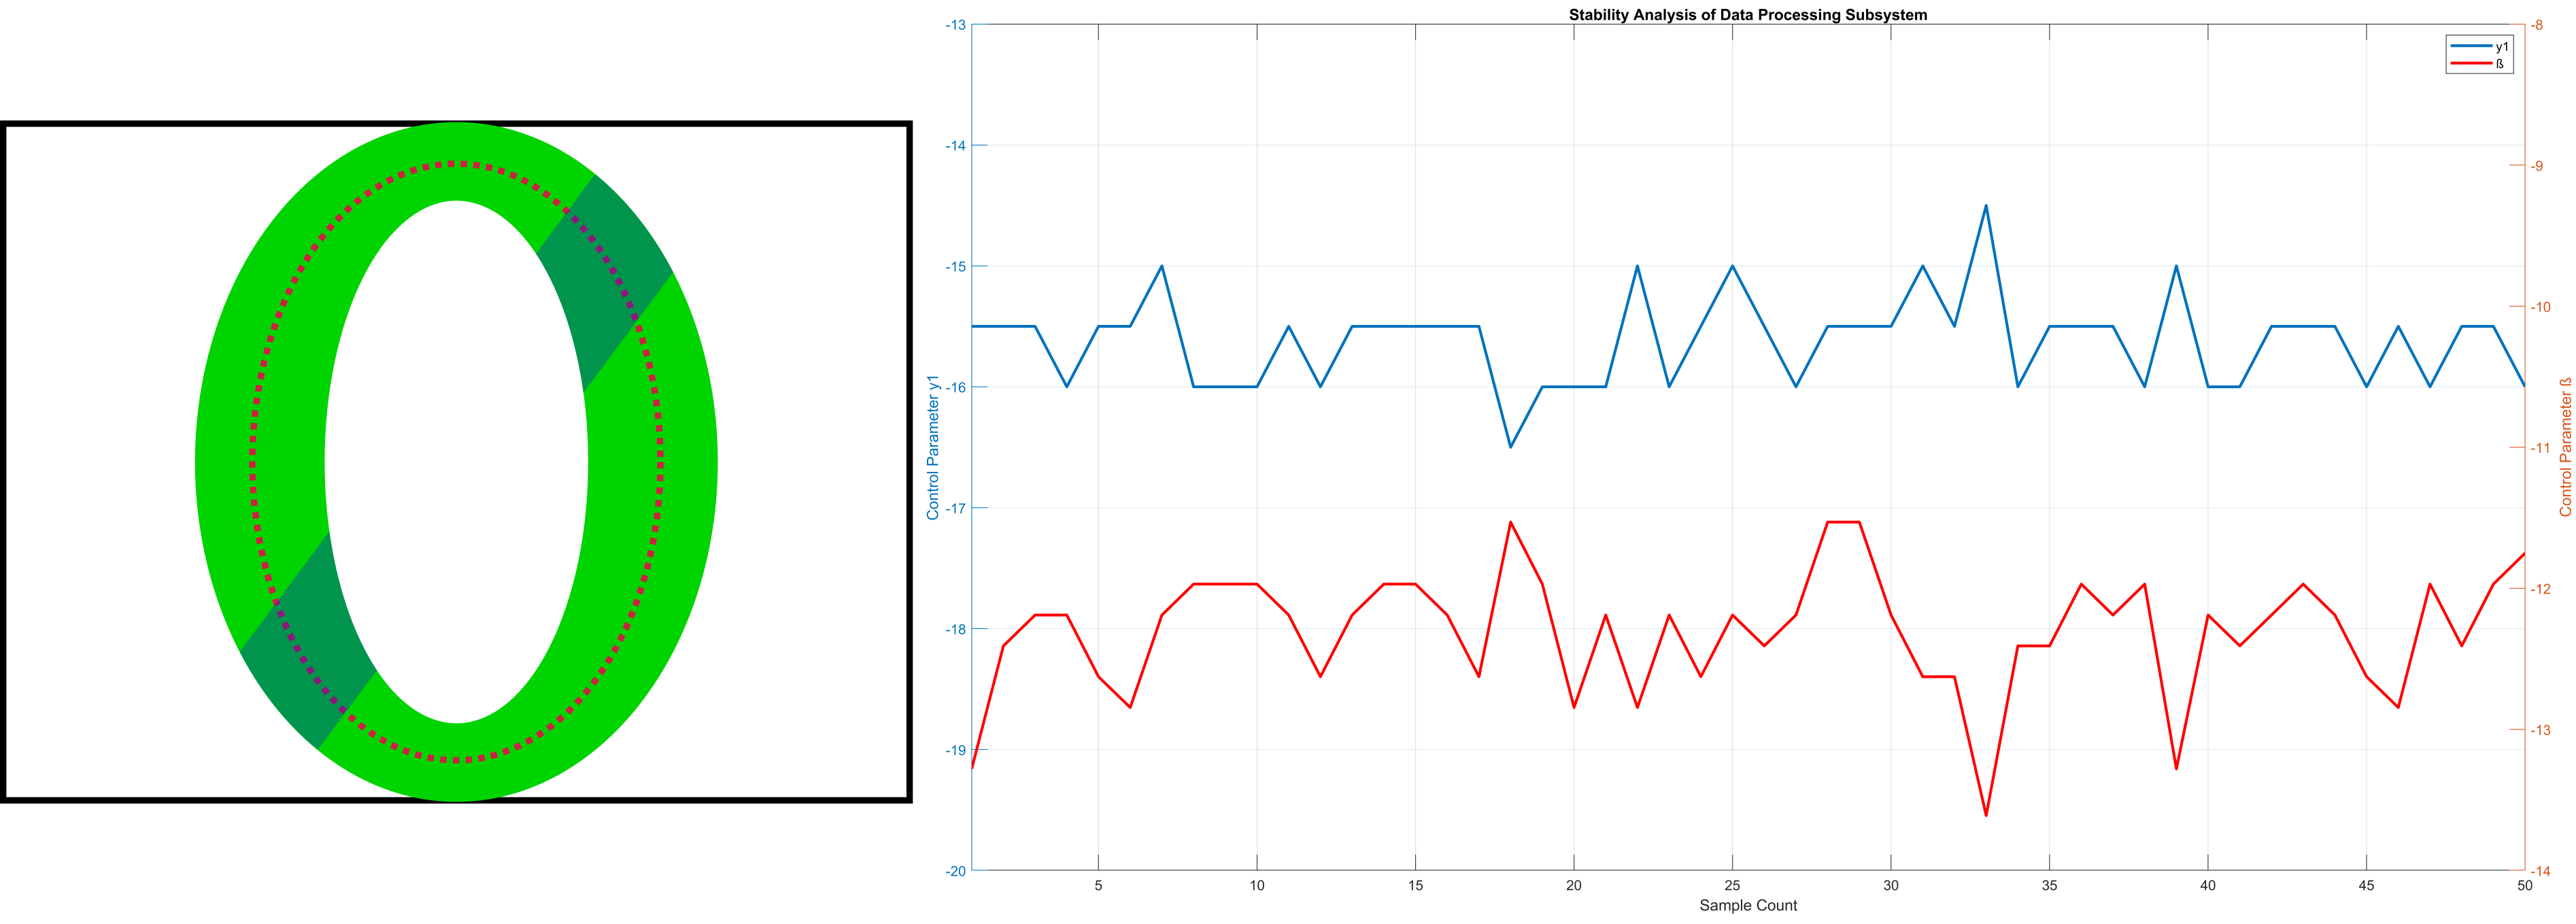
\includegraphics[width=.95\textwidth,center]{images/stabilityTestS}
	
	\caption{ Left: The Vehicle is placed on Bended Area.\\ Right: The Control Outputs \label{fig:stabilityTestS-dist} }
	
\end{figure}	
\begin{figure}[h!]
	
	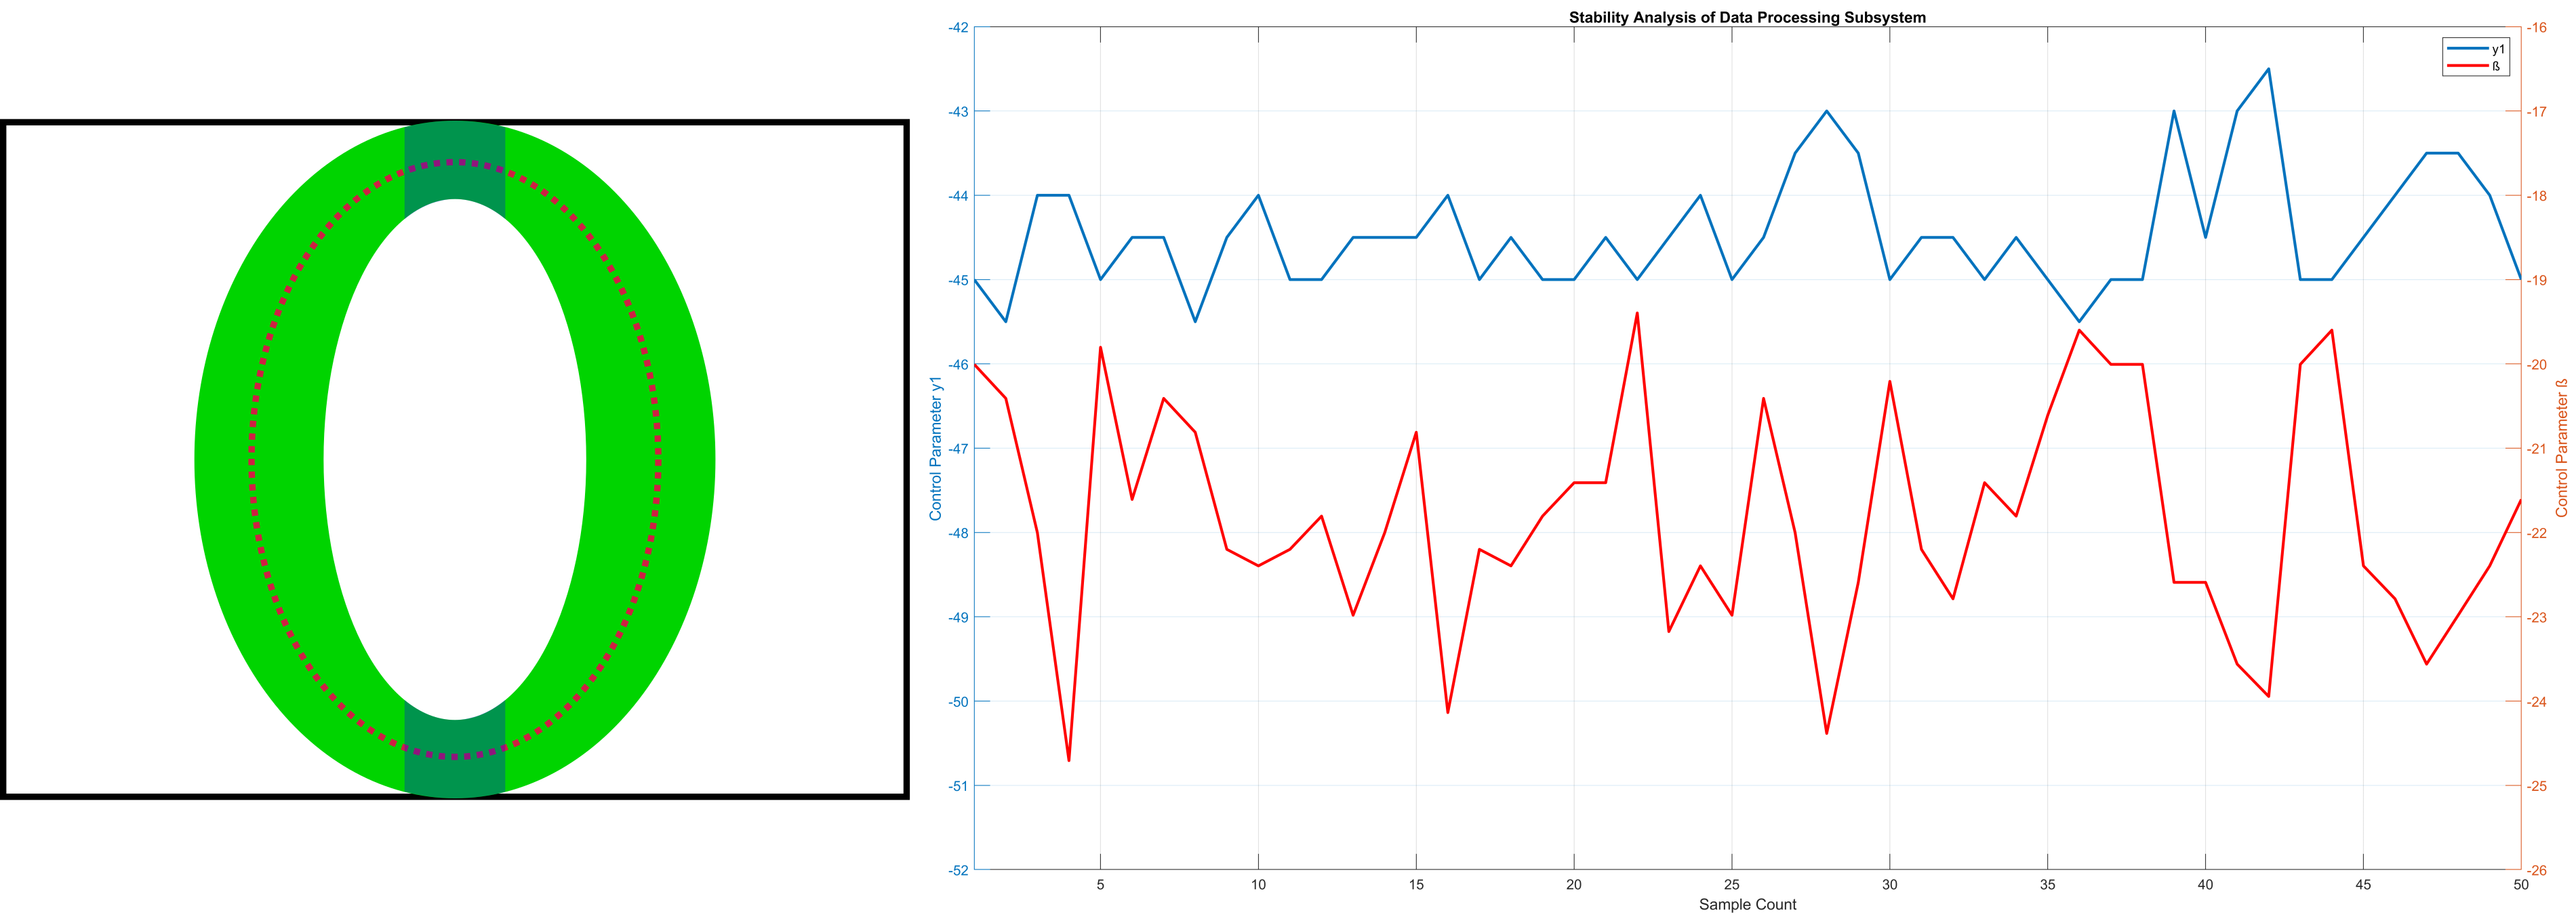
\includegraphics[width=.95\textwidth,center]{images/stabilityTestU}
	
	\caption{ Left: The Vehicle is placed on Curved Area.\\ Right: The Control Outputs \label{fig:stabilityTestU-dist} }
	
\end{figure}	




%%%%%%%%%%%%%%%%%%%%%%%%%%%
\newpage
\subsection {PID Controller Subsystem Tests and Results}	

\begin{enumerate}
	
	
	
	\item PID Parameters Tuning Test :	 \label{test:a}	
	
	\begin{enumerate}
		\item Charge each Li-Po battery cell  up to 3.95 V
		\item Check the regulator output voltage, if it is not at 10.44, play with internal potentiometer to make it so  
		\item Start the data processing from Raspberry Pi
		\item Equate $K_d$ and $K_i$ values to zero
		\item Give the power to the motors  
		\item Sweep the $K_p$ value to follow the part wityh unstable, oscillatory behaivor
		\item Sweep the $K_d$ value to damp these oscillation, stop before the system become unstable
		\item Sweep the $K_i$ value to reduce steady-state error, stop before the system become unstable	
		\item Observe the behaviour of the vehicle  
		\item If the vehicle is able to complete the path at ten consecutive lap, the controller can be classified as working.  
	\end{enumerate}
	
	
	\item Bump Test for Distance Control: \label{test:b}	
	
	\begin{enumerate}
		\item Set-up a lane as in \textit{Figure~\ref{fig:bump-dist}}.
		\item Make the necessary connection between motors Arduino and data processing unit  
		\item Drive the vehicle with PID parameters to be tested.
		\item Collect the distance error between the center of the lane and current position of the vehicle.
		\item Plot the time vs distance graph at Matlab using the collected distance errors.
		\item Calculate necessary performance parameters from the plot.
	\end{enumerate}
	
	
	\begin{figure}[H]
		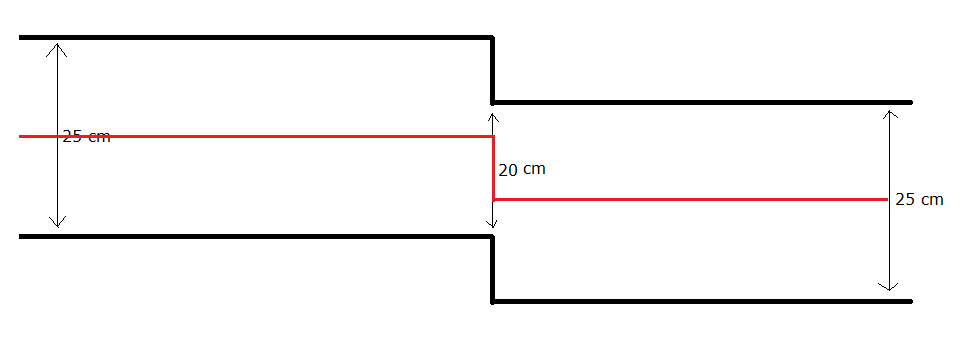
\includegraphics[width=0.75\textwidth,center]{images/bump_test_dist}
		\caption{Bump Test for Distance Control \label{fig:bump-dist} }
	\end{figure}		
	
	
	
	\item Tracking a Path with Obstacles Test:	\label{test:e}	
	
	\begin{enumerate}
		\item Make the necessary connection between motors Arduino and data processing unit  
		\item Place the vehicle to the desired path with obstacles  
		\item Observe the behaviour of the vehicle  
		\item If the vehicle can follow the path and compensate the steady state errors due to obstacles without showing oscillatory behaviour and in  less than 2 seconds, the result of the test can be considered as success.  
		
	\end{enumerate}
	
	\item Path Tracking Test with Physical Disturbances: \label{test:f}	
	
	\begin{enumerate}
		\item Make the necessary connection between motors Arduino and data processing unit  
		\item Place the vehicle to the desired empty path   
		\item Observe the behaviour of the vehicle  
		\item If the vehicle can follow the path and compensate the steady state errors due to physical disturbance without showing oscillatory behaviour and in less than 2 seconds, the result of the test can be considered as success.  
	\end{enumerate}
	
	\item Sampling Time Consistency Test: \label{test:g}	
	
	\begin{enumerate}
		\item Make the necessary connection between motors Arduino and data processing unit  
		\item Place the vehicle to the desired empty path   
		\item Record the data proccessing time of each frame to a text file.
		\item Plot the time vs processing time plot.
		\item If the processing time, i.e., sampling time of the plant is oscillating inside $10\%$ band of thesampling time value used by PID controller subsystem, the test can be classified as success.
	\end{enumerate}
		
\end{enumerate}
	
	
	\subsubsection*{Results of PID Controller Subsystem Tests}
	
	The resuts for \textit{PID Parameters Tuning Test} can be seen at \textit{Figures~\ref{fig:ccwLapTime}~\&~\ref{fig:cwLapTime}}. The results satisfied the claimed succes requirement by completing at least 20 consecutive lap in one run for both direction. The controller also showed satisfactory performance to other test.
	
	\begin{figure}[H]
		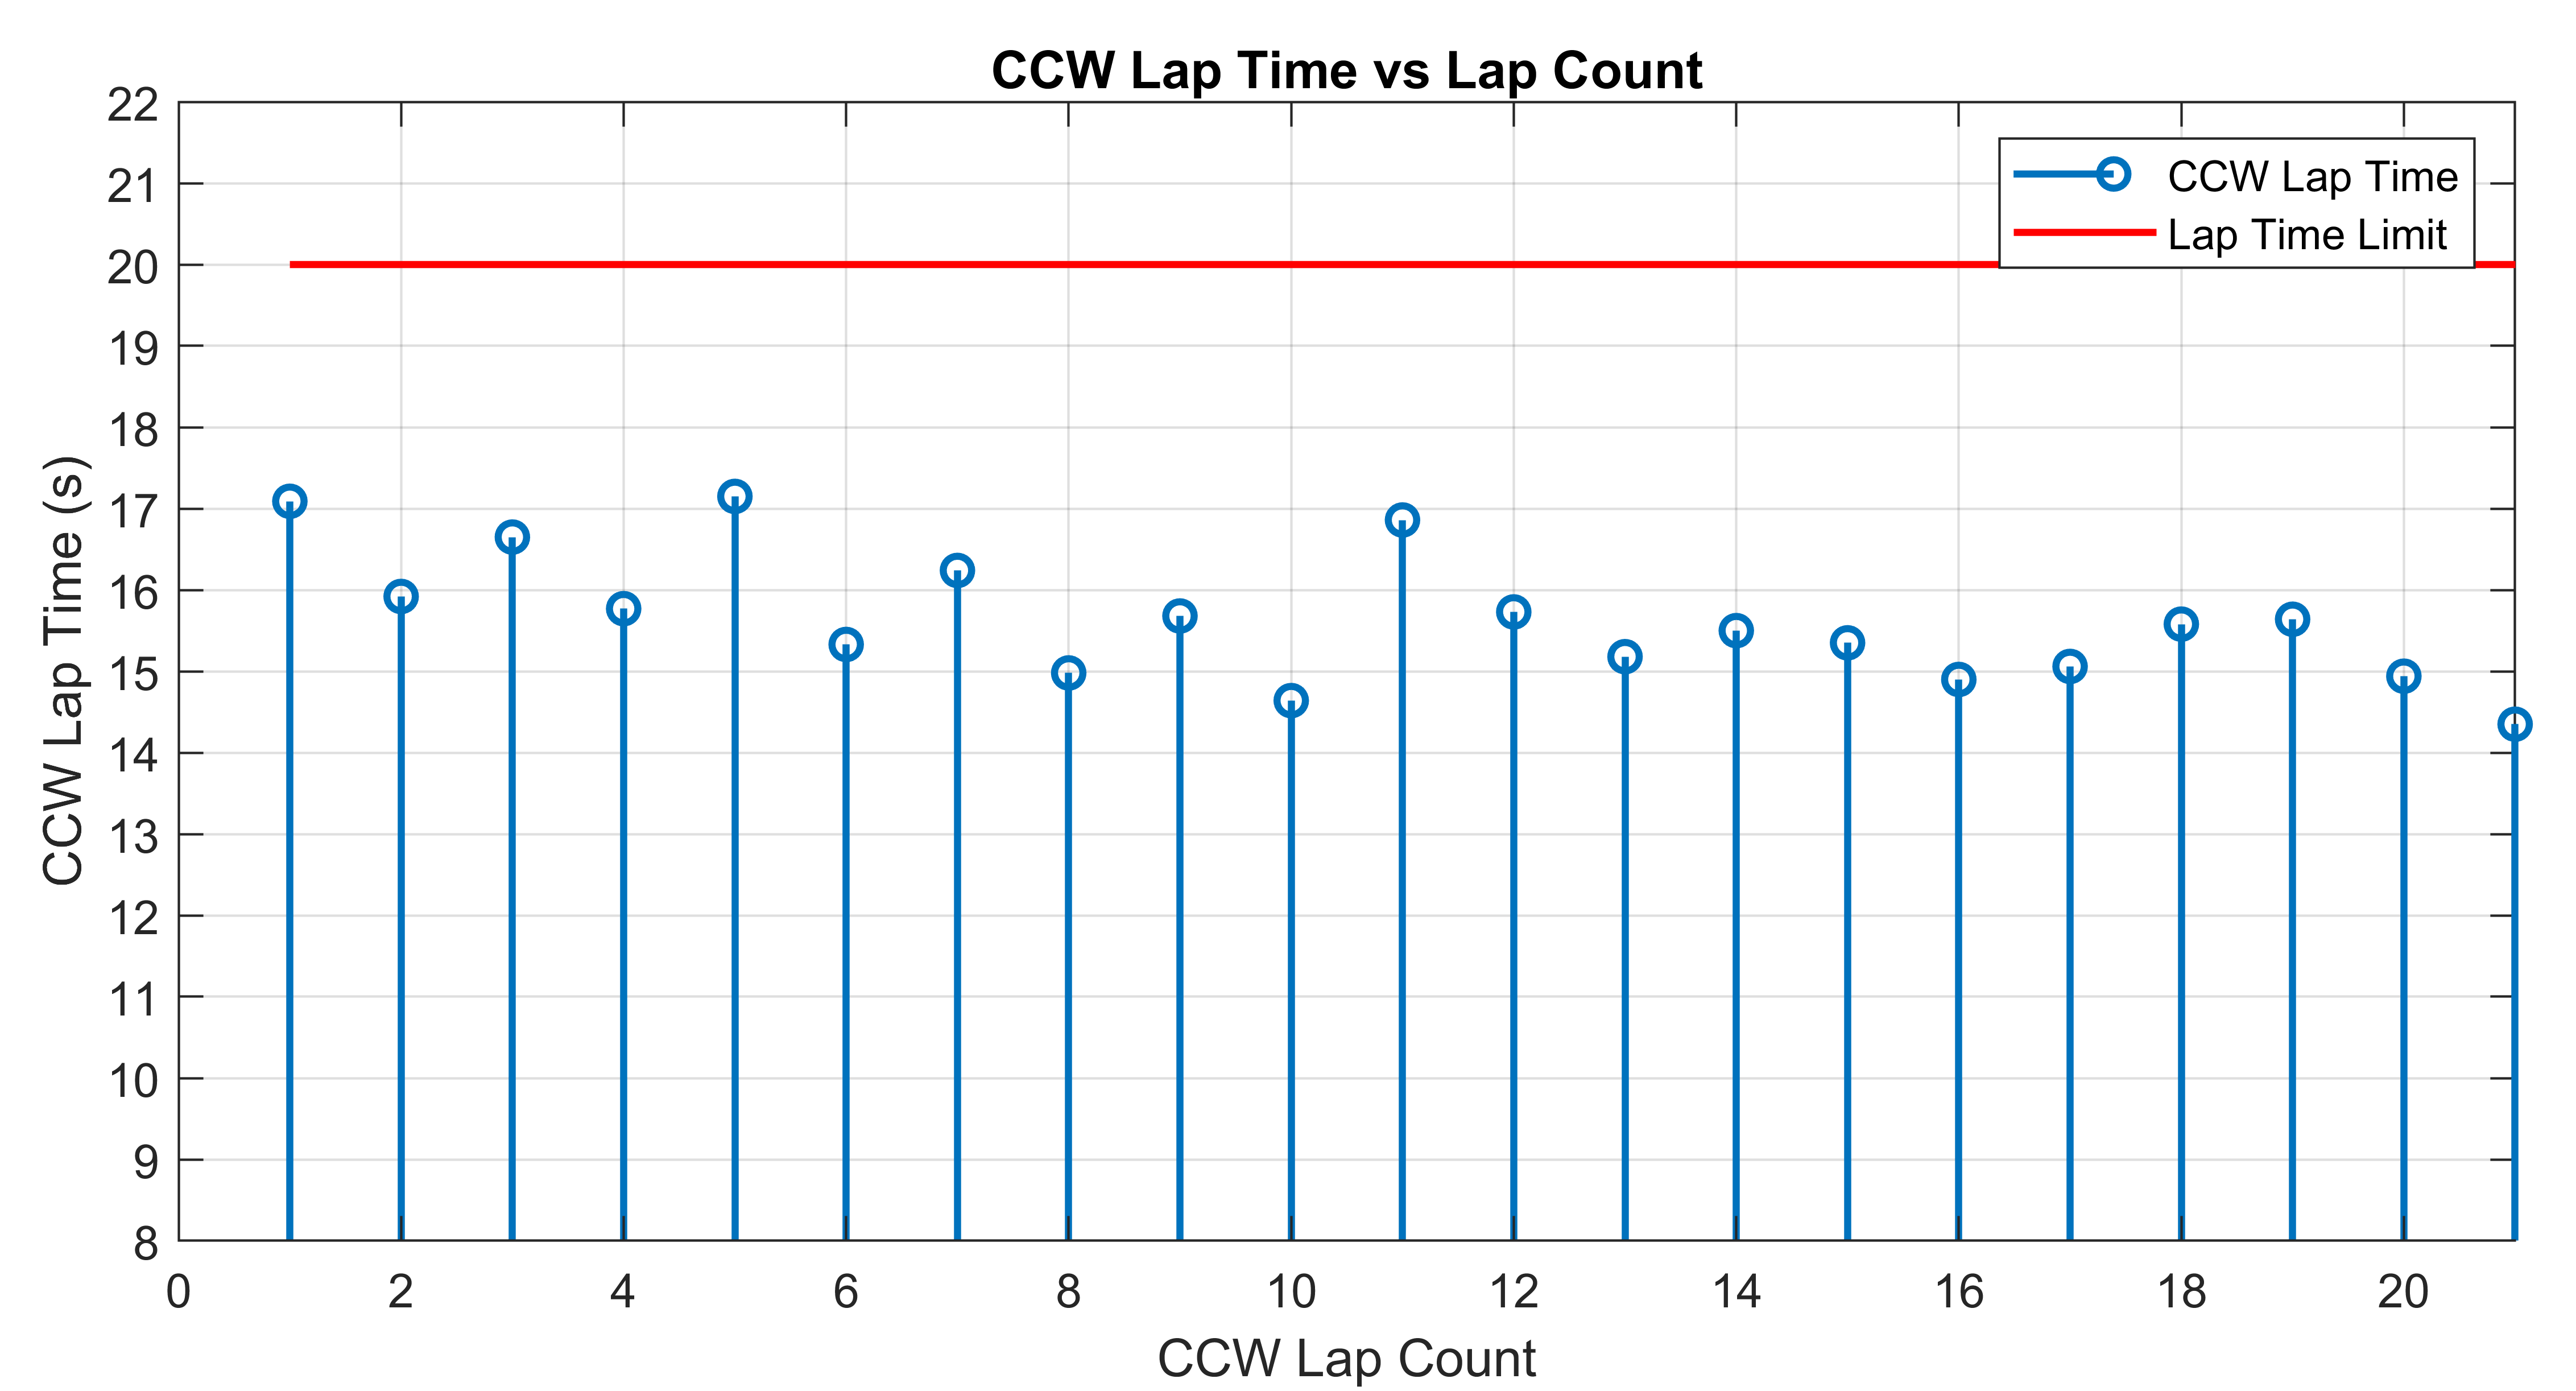
\includegraphics[width=\textwidth,center]{images/ROT_ROI/ccwLapTime_crop}
		\caption{\label{fig:ccwLapTime} Results of PID Tune Test for CCW Movement on the Path}
	\end{figure}
	
	\begin{figure}[H]
		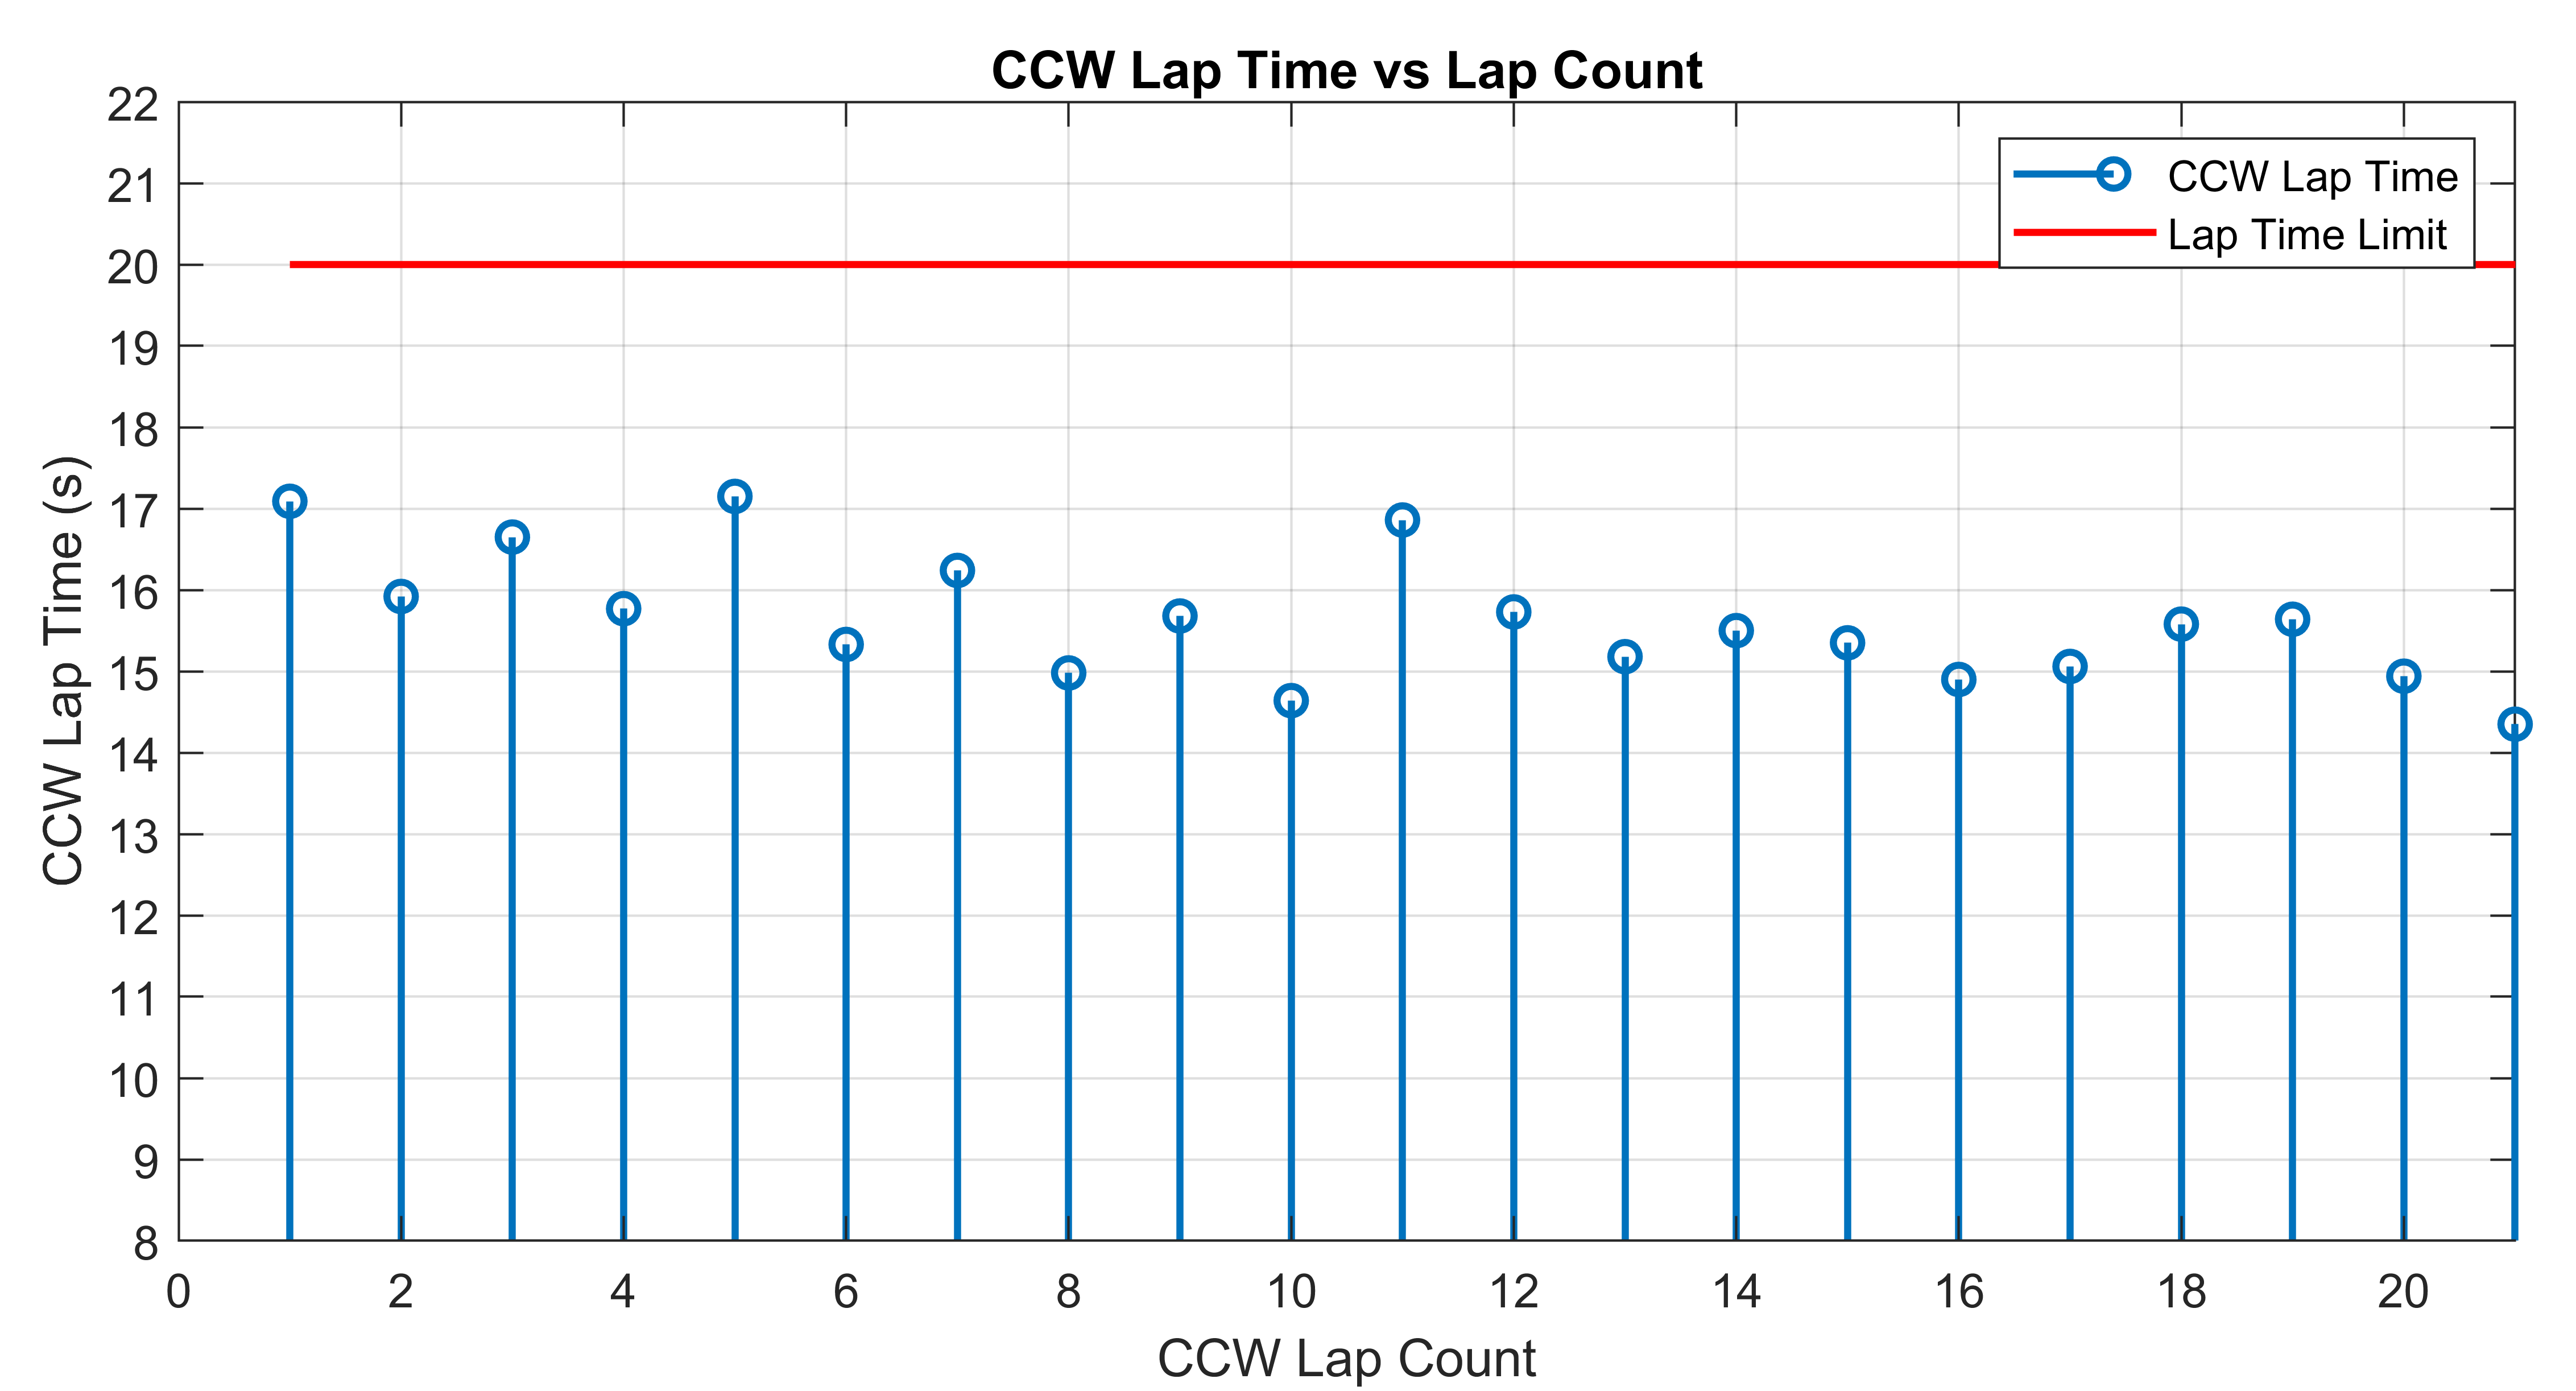
\includegraphics[width=\textwidth,center]{images/ROT_ROI/ccwLapTime_crop}
		\caption{\label{fig:cwLapTime} Results of PID Tune Test for CW Movement on the Path}
	\end{figure}
	
	The resuts for \textit{ Sampling Time Consistency Test} proved the stability of the \textit{Data Processing Unit} and the relaibility of the PID Controller Subsystem, since the sampling time for the discrete time systems is very crucial and should be consistent at all time. 
	
	\begin{figure}[H]
		\includegraphics[width=\textwidth,center]{images/ROT_ROI/ProcessTime_crop}
		\caption{Sampling Time Consistency Test Result }\label{fig:blockdiagram}
	\end{figure}


%%%%%%%%%%%%%%%%%%%%%%%%%%%


\subsection {Internal Communication Subsystem Tests and Results}

\begin{enumerate}

\item Data Retrieval Test

\begin{enumerate}

\item Generate data on Raspberry Pi in a rate that reflects the time consumed of Data Processing subsystem. This will yield a realistic data rate.  

\item Send random text data to Arduino.  

\item Do the initial integration between Arduino and Raspberry Pi.  

\item Send data from Raspberry Pi to Arduino.  

\item Increase data speed to the specified data rate.  

\item Check the accuracy of the retrieved data. 

\end{enumerate}

\end{enumerate}


\subsubsection*{Results of Internal Communication Subsystem Tests}


	%The results are positive after all the necessary adjustments are done. The test is also repeated with the real lane detection algorithm and the real time sent data is read from LCD display connected to Arduino. The system was working properly at the rate at which lane detection algorithm produces data.





%%%%%%%%%%%%%%%%%%%%%%%%%%%

\subsection {External Communication Subsystem Tests and Results}


\begin{enumerate}
	
	
	\item Catching the Opponent Test:
	
	
	\begin{enumerate}
		
		\item Create an Ad-Hoc Wi-Fi from Pi so that opponent can connect (or connect to opponent's Ad-Hoc Wi-Fi)
		
		\item Enter opponent's ID number and host type (server or client) to the terminal
		
		\item Approach the opponent less than 5 cm
		
		\item The test result can be considered as success if blue LED is lid  after RED LED without significant delay(i.e. no crashing) and the device immediately stops.
		
	\end{enumerate}		
	
	
	\item Caught by the Opponent Test:
	
	
	\begin{enumerate}
		
		\item Create an Ad-Hoc Wi-Fi from Pi so that opponent can connect (or connect to opponent's Ad-Hoc Wi-Fi)
		
		\item Enter opponent's ID number and host type (server or client) to the terminal
		
		\item Let the opponent to approach less than 5 cm
		
		\item The test result can be considered as success if green LED is lid without significant delay(i.e. no crashing) and the device immediately stops.
		
	\end{enumerate}	
	
	\item Rejected by the Opponent Test:
	
	
	\begin{enumerate}
		
		\item Create an Ad-Hoc Wi-Fi from Pi so that opponent can connect (or connect to opponent's Ad-Hoc Wi-Fi)
		
		\item Enter opponent's ID number and host type (server or client) to the terminal
		
		\item Place an object in front of the front sensor in a distance less than 5 cm
		
		\item The test result can be considered as success if RED LED is lid without significant delay and the device does not stop.
		
	\end{enumerate}	
	
	\item Rejecting the Opponent Test:
	
	
	\begin{enumerate}
		
		\item Create an Ad-Hoc Wi-Fi from Pi so that opponent can connect (or connect to opponent's Ad-Hoc Wi-Fi)
		
		\item Enter opponent's ID number and host type (server or client) to the terminal
		
		\item Let the opponent to place object  in front of the front sensor in a distance less than 5 cm
		
		\item The test result can be considered as success if yellow LED is lid without significant delay and the device does not stop.
		
	\end{enumerate}	
	
	
	
	\subsubsection*{Results of External Communication Subsystem Tests}
	
	As mentioned in the design description section of the external communication subsystem, there exists a waiting period to receive messages from opponent. This duration, which is also called timeout, directly affects the frequency of the front sensor readings, because it is spent between consecutive readings. In the test results, setting it to high values(higher than 1s) gives good results in  \textit{Caught by the Opponent Test}, since it increases the probability to receive messages from the opponent. However, it results in crashing in \textit{Catching the Opponent Test}, because of the latency of the sensor reading. On the other hand, setting very low timeout(lower than 100 ms) speeds up the process and yields successful results in \textit{Catching the Opponent Test}. However, it decreases the probability of getting messages from the opponent, so \textit{Caught by the Opponent Test} fails. After test results, it is decided that 0.3 seconds is an appropriate value for timeout. By doing so, the probability of crashing is made lower and receiving messages is made higher.
	
\end{enumerate}


%%%%%%%%%%%%%%%%%%%%%%%%%%%


\subsection {Direction Subsystem Tests and Results}

	\begin{enumerate}
		\item Straight Drive Test: \label{test:a1}	
		\begin{enumerate}
			\item Make the necessary connections between motors, motor controller and the Arduino  
			\item Set the PWM values of the motors equal  
			\item Observe the behaviour of the motors  
			\item Increase the PWM value of the slower motor until a point the vehicle can go in a straight line.
			\item Record this PWM difference to use in PID controller subsystem
		\end{enumerate}

		\item Circular Drive Test: \label{test:b1}	
		\begin{enumerate}
			\item Make the necessary connections between motors, motor controller and the Arduino  
			\item Desired curvature is decided  
			\item  According to motion of the vehicle PWMs of the motors are set  
			\item  PID parameters are set according to this test
		\end{enumerate}
	\end{enumerate}

\subsubsection*{Results of Direction Subsystem Tests}

	The results of \textit{Tests~\ref{test:a1} \& \ref{test:b1}} proposed in \textit{Section 3} revealed to the team that, the differential drive method is capable of returning as desired and can keep up with the lane to be followed. Thereby, the design finalized with differential drive vehicle.


%%%%%%%%%%%%%%%%%%%%%%%%%%%


\subsection {Speed Subsystem Tests and Results}

\begin{enumerate}
	
	
	\item Determination of Minimum Base Speed Coefficients Test: \label{test:a2}		
	\begin{enumerate}
		\item Charge each Li-Po battery cell  up to 3.95 V
		\item Check the regulator output voltage, if it is not at 10.44, play with internal potentiometer to make it so  
		\item Start the data processing from Raspberry Pi
		\item Use the PID parameter values determined at \textit{Test~\ref{test:a}}
		\item Give the power to the motors  
		\item Sweep the $K_{min1}$ value to find large enough minimum PWM value so that the vehicle do not leave the lane at corners
		\item Sweep the $K_{min2}$ value to find large enough minimum PWM value that the vehicle do not speed up too much on straight sections of the path so that it does not enter the corners too fast.
		\item Observe the behaviour of the vehicle  
		\item If the vehicle is able to complete the path at ten consecutive lap, the coefficients can be classified as working. Record these values  
	\end{enumerate}
	
	\item Determination of Maximum Base Speed Coefficients Test: \label{test:a2}		
	\begin{enumerate}
		\item Charge each Li-Po battery cell  up to 3.95 V
		\item Check the regulator output voltage, if it is not at 10.44, play with internal potentiometer to make it so  
		\item Start the data processing from Raspberry Pi
		\item Use the PID parameter values determined at \textit{Test~\ref{test:a}}
		\item Give the power to the motors  
		\item Sweep the $K_{max}$ value to find small enough minimum PWM value so that the vehicle do not speed up too much on straight sections of the path so that it does not enter the corners too fast.
		\item Observe the behaviour of the vehicle  
		\item If the vehicle is able to complete the path at ten consecutive lap, the coefficient can be classified as working.  
	\end{enumerate}
	
	\item Determination of Slow Down Coefficients Test: \label{test:a2}		
	\begin{enumerate}
		\item Charge each Li-Po battery cell  up to 3.95 V
		\item Check the regulator output voltage, if it is not at 10.44, play with internal potentiometer to make it so  
		\item Start the data processing from Raspberry Pi
		\item Use the PID parameter values determined at \textit{Test~\ref{test:a}}
		\item Give the power to the motors  
		\item Sweep the $K_1$ value to find large enough value so that the vehicle slow down properly but does not saturate to the minimum PWM limit
		\item Observe the behaviour of the vehicle  
		\item If the vehicle is able to complete the path at ten consecutive lap, the coefficient can be classified as working.  
	\end{enumerate}
	
\end{enumerate}
	
	\subsubsection*{Results of Speed Subsystem Tests}
	
	The result of each parameter tuning test can be found at \textit{Figure~\ref{fig:baseSpeedExp}}
	
	\begin{figure}[h]
		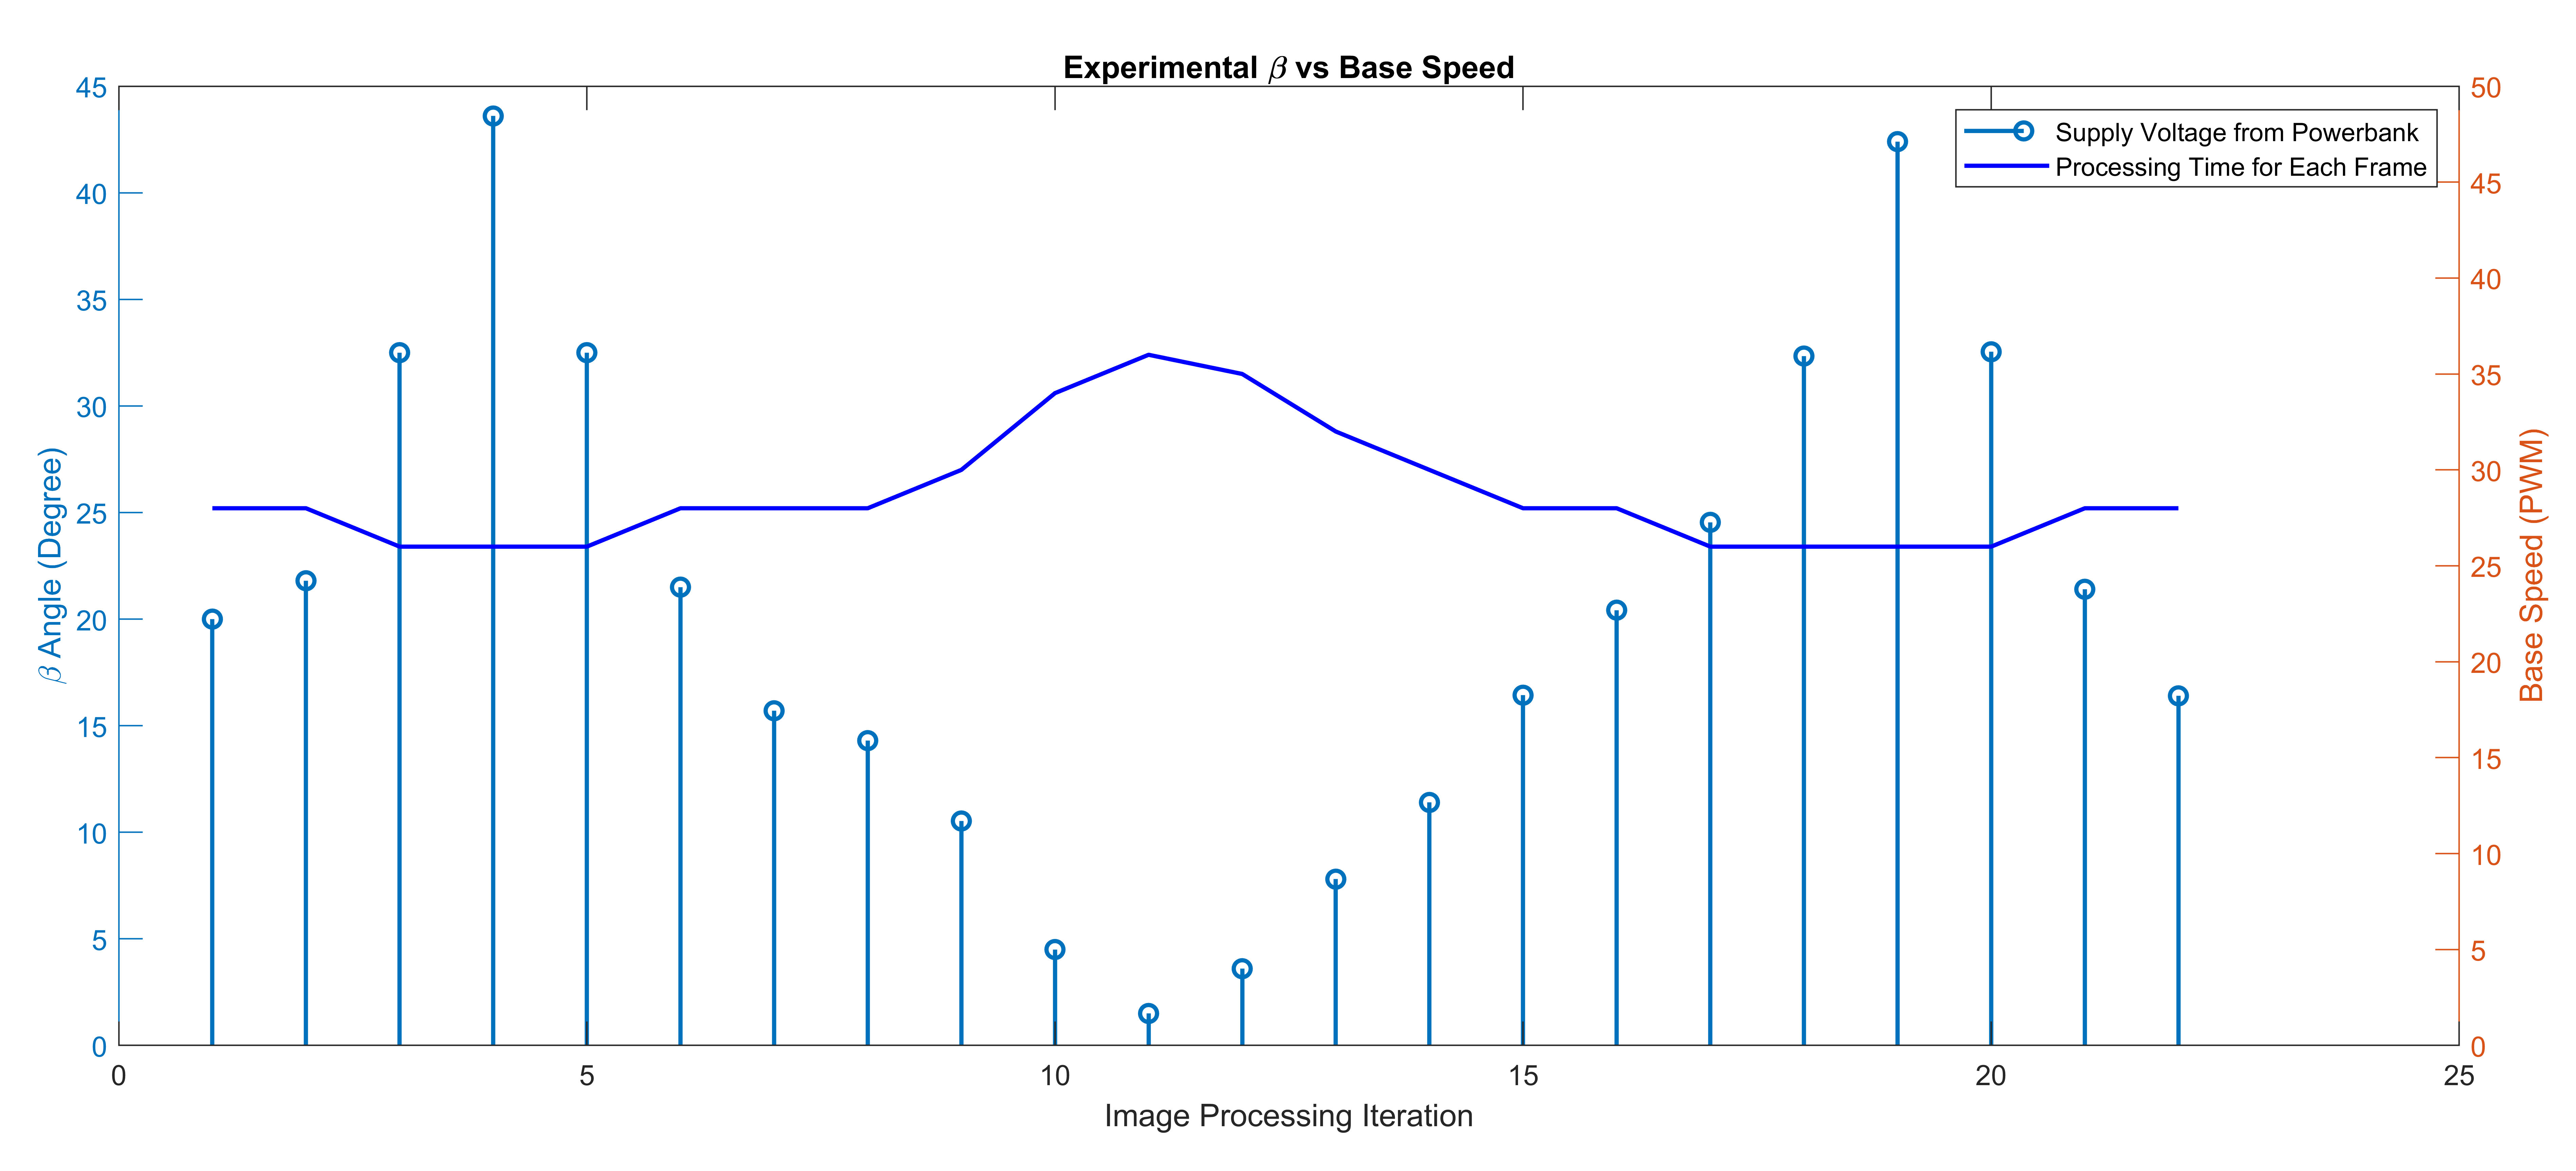
\includegraphics[width=\textwidth,center]{images/ROT_ROI/baseSpeedExp_crop}
		\caption{Experimental Base Speed PWM vs Experimental $\beta$ Angle}\label{fig:baseSpeedExp}
	\end{figure}
	
	



%%%%%%%%%%%%%%%%%%%%%%%%%%%

\newpage

\subsection{Wheels Subsystem Tests and Results} 


\begin{enumerate}

\item {Handling Test:} 

\begin{enumerate}

\item  Place the vehicle on the path

\item Apply a horizontal force

\item Observe the behaibour 

\item If the vehicle is slipping, the test can be considered to be failure. If not, the the test result can be considered as success. In other word, friction between road and wheel should greater than road and ground. 


\end{enumerate}

\end{enumerate}


\subsection {Motors Subsystem Tests and Results} 


\begin{enumerate}

\item {Torque Test:} 

\begin{enumerate}

\item Fix the motor at horizontal position with respect to ground  

\item Attach an object of one kilogram  

\item Contact the seller for more information 

\end{enumerate}


\end{enumerate}




\subsubsection*{Results of Motion System Tests}

	%After tests, handling capability of the system is approved. However, although motors are quite well with high PWM, their low PWM performance cause some problems. Therefore, motor subsystem could need a revision.





%%%%%%%%%%%%%%%%%%%%%%%%%%%


\subsection {Chassis Subsystem Tests and Results}

\begin{enumerate}

\item Inertia test: 

\begin{enumerate}

\item Prepare a straight path

\item Power up the vehicle 

\item Execute the edge detection and control algorithm

\item Give different type of disturbances 

\item Observe the deviation from straight line

\item Repeat the process with different component configurations

\end{enumerate} 

\end{enumerate}





%%%%%%%%%%%%%%%%%%%%%%%%%%%



\subsection {Printed Circuit Board Subsystem Tests and Results}


\begin{enumerate}

\item Short test: Aims to check all the wanted connections are present. The test procedure is as follows:

\begin{enumerate} 

\item Open multimeter for short circuit test  

\item Find the ends of each routing 

\item Check the continuity using multimeter probes

\item Check if there is any unwanted short circuit

\item If exist, eliminate

\end{enumerate}


\end{enumerate}

\subsubsection*{Results of Structure System Tests}

	%As mentioned in Section 3, the disturbances applied on the vehicle and the deviation is between the levels that can be handled by other algorithms although some improvements are still needed. Furthermore, newly-designed chassis added rigidity to the structure which in turn provides better test results




\section{Budget}
		
	In this section spendings of the project will be investigated under two part. Fistly, real spendings will be analyzed and secondly, the cost of reproducable product will be investigated.

	\subsection{Actual Expenditures}
	
		Besides the component spendings spesified at \textit{Table~\ref{tab:totalcost}}, $100~\$$ worth mechanical components, such as rechargeble drill and approximately $100~\$$ worth electrical components from porevious term projects were utilized throughout the project. Thereby, a total of approximate $616.5~\$$ budget and  1700 man-hour were spent on this project.
		
		\begin{table}[H]
			\centering
			\caption{Total Spendings for the Project}
			\begin{tabular}{c|c}
				$$Component$$ &  $$Approximate Spendings (in Dollar)$$  \\ \hline
				Raspberry Pi & 50   \\ \hline
				Raspberry Pi Camera & 47   \\ \hline
				Chassis $\&$ Mechanical Components & 45   \\ \hline
				Arduino  & 20 \\ \hline
				DC Motor $\&$ Wheel & 100 \\ \hline
				Motor Driver and Regulator &  9.5 \\ \hline
				Powerbank & 25 \\ \hline
				Li-po Battery  &  23 \\ \hline
				Sensor $\&$ Cable & 60 \\ \hline
				Other Spendings & 37 \\ \hline
				Total Project & 416.5
			\end{tabular} 
			\label{tab:totalcost}
		\end{table}
		
	\subsection{Cost Analysis of Reproducible Product}

	Cost anaysis for the \textbf{Kobra 6.5} can be investigated under \textit{Table~\ref{tab:cost}}. The reproducible vehicle costs under 200 dollar as stated by the project requirements. However, it should be noted that the 200 dollar budget does not cover additional expenses such as li-po battery charger and micro-USB chager.

	
	\begin{table}[H]
		\centering
		\caption{Cost Analysis for the Project}
			\begin{tabular}{c|c|c}
			$$Component$$ & $$Number$$ & $$Total Price (in Dollar)$$  \\ \hline
			Raspberry Pi 3B & 1 & 47   \\ \hline
			Waveshare Raspberry Pi Camera (D) & 1 & 22   \\ \hline
			Chassis Components & 1 & 13   \\ \hline
			Arduino Nano & 1 &  4.8 \\ \hline
			Polulu 150:1 6 V 200 RPM DC Motor & 2 & 42 \\ \hline
			Bond Silicon Wheel & 2 & 8 \\ \hline
			Motor Driver and Voltage Regulator & 1 &  4 \\ \hline
			Xiaomi 10000 mAh Mi Powerbank (Ver 3) & 1 & 12 \\ \hline
			ProFuse 11.1 V 1750 mAh Li-po Battery  & 1 & 23 \\ \hline
			Polulu VL6180X ToF Distance Sensor & 2 & 17 \\ \hline
			LED headlight/LED & - & 0.2 \\ \hline
			Styrofoam, Glue $\&$ Cardboard & - & 6.5 \\ \hline
			Total Project & - & 199.5 
		\end{tabular} 
		\label{tab:cost}
	\end{table}
	
	As can be reffered from the \textit{Table~\ref{tab:cost}}, some component modification were made for the final design after conceptual design review report. For example, DC motors were replaced with the ones having lower rpm values, or powwerbank as replaced with the one having quick charge capabilities to elliminate unidealities in performance.

	\section{Power Analysis}
	
	\begin{table}[H]
		\centering
		\caption{Estimated Cost Analysis for the Project}
		\begin{tabular}{c|c|c|c|c}
			$$Component$$ & $$\specialcell{Current\\ (Avg),A}$$ & $$\specialcell{Power\\(Avg),W}$$ & $$\specialcell{Current\\(Max),A}$$ & $$\specialcell{Power\\(Max),W}$$ \\ \hline
			Raspberry Pi 3B & 0.85 & 4.25 & 2.5 & 12.5   \\ \hline
			Arduino Nano & 80m &  0.4 & 0.2 & 1 \\ \hline
			DC Motors \& Motor Driver & 0.4 & 4.8 & 1.1 & 12.12 \\ \hline
			Distance Sensor & 19m & 62.7m & 40m & 132m \\ \hline
			Total  &  1.52m & 9.153 & 3.84 & 25.75         
		\end{tabular} 
		\label{tab:power}
	\end{table}

		The \textit{Table~\ref{tab:power}} shows the consumption under regular case and extreme case. If extreme scenario is considered, full power consumption of Raspberry Pi is supplied from powerbank while motors are supplied by Li-Po battery as can be seen from the \textit{Figure~\ref{fig:elec}}. Also, sensors and Arduino are supplied from Pi because they do not have high demand. Powerbank has two output could supply 2.5A for 5V output, so Pi could supply in the worst case.
		
		\begin{figure}[H]
			\includegraphics[width=\textwidth,center]{images/elec_arch2}
			\caption{Electrical Architecture of the Project}\label{fig:elec}
		\end{figure}
		
		Li-Po battery has these specs: 1750 mAh 11.1V 3S 25C, so it can supply 43 ampere constants during discharge although the motors demand 1.1 ampere at stall condition. 

		 All in all, sources are completely enough for consumption even in the worst case conditions. Although, previous chosen powerbank, in therory, was capable of producing enough power for Raspberry Pi, in reality, its fluctiations in voltage output caused undesired low voltage warnings from Raspberry Pi which leads to closing of two cores of its cpu. As a result, this fluctiations in voltage caused undesired fluctiations in processing time as can be seen \textit{Figure~\ref{fig:processTime}}  

	\begin{figure}[h]
		\includegraphics[width=\textwidth,center]{images/ROT_ROI/voltageSupply_crop}
		\caption{The Relation Between Supply Voltage from Powerbank vs Process Time}\label{fig:processTime}
	\end{figure}


	\newpage

	\section{Deliverables}
		Deliverables of the product are listed as follows;
		\begin{itemize}
			\item Kobra 6.5  
			\item Li-Po batteries (3S 11.1 V)
			\item Power bank (Li-Ion 10 000 mAh)
			\item Race Track 
			\item Flash stick with sofware 
			\item User Manual 
			\item USB Cable
		\end{itemize} 
	\section{Discussions}
		This sections presents a discussion on several things such as safety issues, application areas and environmental effects of the final product.
	
	\subsection{Safety Issues}
		Safety is the most important consideration of every project, so during design, it is considered after every solution step. Product is tested under tougher than general customer use such as no cooling of raspberry pi or constant usage of 8 hours etc. 
		
		The most dangerous sections are Li-Po battery, Arduino and Motor driver, in other words, where the current flows. Although Li-Po battery is dangerous for a toy, in design it placed between two layers of chassis to protect it from damage or direct sun light. Besides of this, these three components share the same ground path, so charging cycle is tested, additionally, to avoid any ground loop. 
		
		Raspberry pi is the main computation component of Kobra 6.5, so it has some overheating issues, especially hot days. Therefore, It is cooled by FAN and heat sink system. Additionally, it’s power totally isolated from dangerous high current line (as mentioned previous paragraph) to eliminate any over voltage/current condition. 
		
		Thanks to these considerations, if there is no over charging condition of Li-Po battery, this product can be used totally safely.  
		

	\subsection{Application Areas}
		At first sight, this project seems like a toy for children. As an RC car, two children can play with each other for fun. However, when project analyses in detail such as considering sub-systems, it is a small model of unmanned vehicle which has anti collusion and obstacle avoidance features. Furthermore, with modification of the sub-systems, this project can be evaluating different areas such as lane tracking algorithm can be enhanced to object tracking and this vehicle can follow specified object, or handshake algorithm can be evaluating to IoT applications which requires machine communications.
		
		Considering these applications or more, this project could be primitive model of many specific applications.

	\subsection{Environmental Effects}
		
		The environmental effects can be discussed regarding the material used in body of the car. Chassis and camera arm are all made of plexiglass (PMMA) material. PMMA is a versatile, durable, recyclable and sustainable material. As it has such properties, PMMA based products products have replaced products which were previously made from wood, iron and other natural ingredients. With this way, pressure on natural supplies is decreased. Hence, the acrylic products can be considered as an environment friendly option.

		Regarding the battery, a Li-Po battery is used on the vehicle. Production of Li-Po batteries require lots of chemical and energy. And, what is worse is that there are currently no good programs to recycle lithium-polymer batteries. So, it can be concluded that Li-Po batteries are not environment friendly.


	\section{Conclusion}
	
		This report consists of the summary of the results of entire design effort. For each subsystem, the solutions are explained in detail and the results of the tests are discussed in detail. \\
		
		In especial, overview of the systems is shown in V-Model with the system block diagram. Then, subsystems are given in a detailed manner with clarifications of the final solution, comparison of the CDRR solutions, test steps and test results. The system has been assembled into a final chassis. Mentioned limitations in CDRR are enhanced, as shown in the test result. In addition to this, other non-problematic subsystems’ solutions are frozen. On the other hand, economic constraint which is 200\$ is still higher than cost of the total project. The company believes that power of a company comes from its economic plans. Finally, safety issues, application areas and environmental effects are discussed. \\
		
		This work is  done in a way that it is capable of handling every way, every case and scenario, by the great efforts of the members of DUAYENLER. The company members believe that this project will bring an innovative approach to the design of autonomous cars with its solutions and solution approaches. 

	%\newpage
\newpage



\begin{appendices}


\includepdf[landscape=false,pages=1, scale=0.875,angle=0, label=gannt_chart_app,pagecommand=\section{USER MANUAL}\label{user_man}]{USER_MANUAL.pdf}

\includepdf[landscape=false,pages=2, scale=0.875,angle=0, label=gannt_chart_app,pagecommand=\label{user_man}]{USER_MANUAL.pdf}

\includepdf[landscape=true,pages=1, scale=0.775,angle=0, label=gannt_chart_app,pagecommand=\section{Gannt Chart}\label{gannt_chart_app}]{gantt.pdf}

\includepdf[landscape=true,pages=2-3, scale=0.775,angle=0,pagecommand=]{gantt.pdf}



\end{appendices}








\end{document}


%----samples------

%\begin{itemize}

%\item Item

%\item Item

%\end{itemize}


%\begin{figure}[H]

%\center

%\setlength{\unitlength}{\textwidth} 

%\includegraphics[width=0.7\unitlength]{images/logo1}

%\caption{\label{fig:logo}Logo }

%\end{figure}


%\begin{figure}[H]

%	\setlength{\unitlength}{\textwidth} 

%	\centering

%	\begin{subfigure}{.5\textwidth}

%  		\centering

%  		\includegraphics[width=0.48\unitlength]{images/logo1}

%  		\caption{\label{fig:logo1}Logo1 }

%	\end{subfigure}%

%	\begin{subfigure}{.5\textwidth}

%  		\centering

%		\includegraphics[width=0.48\unitlength]{images/logo2}

%  		\caption{\label{fig:logo2}Logo2}

%	\end{subfigure}

%\caption{\label{fig:calisandegree} Small Logos   }

%\end{figure}


%\begin{table}[H]

%  \centering

% 

%    \begin{tabular}{c|c|c}

%       $$A$$ & $$B$$ & $$C$$ \\ \hline

%       1 & 2 & 3  \\ \hline

%       2 & 3 & 4  \\ \hline

%       3 & 4 & 5  \\ \hline

%       4 & 5 & 6  

%      

%  \end{tabular}

%  \caption{table}

%  \label{tab:table}

%\end{table}


%\begin{table}[H]

%  \centering

% 

%    \begin{tabular}{c|c|c}

%       \backslashbox{$A$}{$a$} & $$\specialcell{ Average deviation \\ after subtracting out the  \\ frequency error }$$ & $$C$$ \\ \hline

%       \multirow{2}{*}{1} & 2 & 3  \\ \cline{2-3}

%        & 3 & 4  \\ \hline

%       3 & \multicolumn{2}{c}{4}  \\ \hline

%       4 & 5 & 6  

%      

%  \end{tabular}

%  \caption{table}

%  \label{tab:table}

%\end{table}

%-----end of samples-----